\باب{حدود اور استمرار}
\جزوحصہء{جائزہ}
تفاعل کی حد کا تصور ان بنیادی تصورات میں سے ایک ہے جو احصاء کو الجبرا اور تکونیات سے علیحدہ کرتا ہے۔

اس باب میں ہم حدود کے تصور کو پہلے وجدانی طور پر اور بعد میں با ضابطہ وضع کرتے ہیں۔ہم حدود کو استعمال کرتے ہوئے تفاعل \عددی{f} میں تبدیلی پر غور کرتے ہیں۔کچھ تفاعل مسلسل تبدیل ہوتے ہیں جہاں \عددی{x} میں چھوٹی تبدیلی، \عددی{f(x)} میں چھوٹی تبدیلی ہی پیدا ہوتی ہے۔دیگر تفاعل میں \عددی{x} کی چھوٹی تبدیلی، \عددی{f(x)} میں چھلانگ یا غیر یقینی تبدیلی  پیدا کر سکتی ہے۔ ہم حدود کو استعمال کرتے ہوئے تفاعل کی ترسیم کے مماثل خطوط متعارف کریں گے۔ اس جیومیٹریائی استعمال کی بنا تفاعل کی تفرق کا تصور پیدا ہو گا۔تفاعل کی تفرق، جس پر اگلے باب میں تفصیلاً غور کیا جائے گا، تفاعل کی تبدیلی کو تعین کرتا ہے۔

\حصہ{تبدیلی کی شرح اور حد}\شناخت{حصہ_حد_تبدیلی_کی_شرح_اور_حد}
اس حصہ میں ہم تبدیلی کی شرح کی دو مثالیں، رفتار اور نمو آبادی متعارف کرتے ہیں جن سے اس باب کا اصل موضوع، حد کا تصور پیدا ہو گا۔

\جزوحصہء{رفتار}
کسی بھی دورانیے میں متحرک جسم کی اوسط رفتار سے مراد اس وقت میں طے فاصلہ تقسیم دورانیہ ہے۔

\ابتدا{مثال}\شناخت{مثال_حد_رفتار_الف}
ایک پتھر \عددی{\SI{100}{\meter}} اونچائی سے گرتا ہے۔ (الف) پہلی دو سیکنڈ میں (ب) پہلی سے دوسری سیکنڈ کے دارانیے  میں پتھر کی اوسط رفتار  کیا ہو گی؟\\
حل:\quad
ہم جانتے ہیں کہ سطح زمین کے قریب ساکن حالت سے گرتا ہوا جسم پہلی \عددی{t} سیکنڈوں میں
\begin{align*}
y=4.9 t^2
\end{align*}
میٹر فاصلہ طے کرتا ہے۔یوں پہلی \عددی{t} سیکنڈ میں اوسط رفتار جاننے کے لئے ہم فاصلہ میں تبدیلی \عددی{\Delta y} کو وقت میں تبدیلی \عددی{\Delta t} سے تقسیم کرتے ہیں۔\\
(الف)\quad
پہلی دو سیکنڈ میں اوسط رفتار
$\tfrac{\Delta y}{\Delta t}=\tfrac{4.9(2)^2-4.9(0)^2}{2-0}=\SI{9.8}{\meter\per\second}$
ہو گی۔\\
(ب)\quad 
پہلی اور دوسری سیکنڈ کے دوران اوسط رفتار
$\tfrac{\Delta y}{\Delta t}=\tfrac{4.9(2)^2-4.9(1)^2}{2-1}=\SI{14.7}{\meter\per\second}$
ہو گی۔
\انتہا{مثال}
%======================= 
\ابتدا{مثال}\شناخت{مثال_حد_رفتار_ب}
پتھر کی رفتار \عددی{t=\SI{1}{\second}} اور \عددی{t=\SI{2}{\second}} پر تلاش کریں۔\\
حل:\quad
ہم وقتی وقفہ \عددی{[t_0,t_0+h]}  پر اوسط رفتار حاصل کرتے ہیں، یعنی:
\begin{align*}
\frac{\Delta y}{\Delta t}=\frac{4.9(t_0+h)^2-4.9t^2_0}{h}
\end{align*}
چونکہ کسی بھی عدد کو صفر سے تقسیم نہیں کیا جا سکتا ہے لہٰذا درج بالا کلیہ میں \عددی{h=0} پر کرتے ہوئے  "لمحاتی رفتار" حاصل نہیں کی جا سکتی ہے۔البتہ اس کلیہ کو استعمال کرتے ہوئے ہم کم سے کم  دورانیے کے لئے اوسط رفتار حاصل کر سکتے ہیں۔یوں \عددی{t_0=1} اور \عددی{t_0=2} کے لئے \عددی{h=0.1,0.01,\cdots} لیتے ہوئے  درج ذیل اوسط رفتار حاصل کیے جا سکتے ہیں۔
\begin{align*}
\begin{array}{lll}
\hline
\multicolumn{1}{c}{h}&\multicolumn{1}{c}{\text{\RL{پر اوسط رفتار}} t_0=1} &\multicolumn{1}{c}{ \text{\RL{پر اوسط رفتار}} t_0=2}\\
\hline
1&14.7&24.5\\
0.1&10.29&20.09\\
0.01&9.84899&19.64899\\
0.001&9.80489&19.60489\\
0.0001&9.800489&19.60049
\end{array}
\end{align*}
آپ دیکھ سکتے ہیں کہ \عددی{t_0=1} کے لئے \عددی{h} کی قیمت کم سے کم کرتے ہوئے اوسط رفتار \عددی{\SI{9.8}{\meter\per\second}}  کے قریب تر ہوتی جاتی ہے جس سے ہم کہہ سکتے ہیں کہ \عددی{t_0=1} پر پتھر کی رفتار \عددی{\SI{9.8}{\meter\per\second}} ہو گی۔اسی طرح \عددی{t_0=2} پر پتھر کی رفتار \عددی{\SI{19.6}{\meter\per\second}} نظر آئے گی۔
\انتہا{مثال}
%============================

\جزوحصہء{اوسط شرح تبدیلی اور سیکنٹ خطوط}
\عددی{x} کے لحاظ سے تفاعل \عددی{f(x)} کی اوسط شرح تبدیلی کو   وقفہ \عددی{[x_1,x_2]}  پر حاصل کرنے کی خاطر ہم \عددی{y} کی قیمت میں تبدیلی،
 \عددی{\Delta y=f(x_2)-f(x_1)} کو \عددی{x} کی قیمت میں تبدیلی \عددی{\Delta x=x_2-x_1=h} سے تقسیم کرتے ہیں۔

\ابتدا{تعریف}
\عددی{x} کے لحاظ سے وقفہ \عددی{[x_1,x_2]} پر \عددی{y=f(x)} کی اوسط شرح تبدیلی درج ذیل ہو گی۔
\begin{align*}
\frac{\Delta y}{\Delta x}=\frac{f(x_2)-f(x_1)}{x_2-x_1}=\frac{f(x_1+h)-f(x_1)}{h}
\end{align*}
\انتہا{تعریف}
%=====================

آپ دیکھ سکتے ہیں کہ وقفہ \عددی{[x_1,x_2]} پر \عددی{f} کی اوسط شرح تبدیلی نقطہ \عددی{N(x_1,f(x_1))} اور نقطہ \عددی{Q(x_2,f(x_2))} سے گزرتے ہوئے خط کی ڈھلوان کے برابر ہے (شکل \حوالہ{شکل_حد_سیکنٹ_ڈھلوان})۔جیومیٹری میں ترسیم پر کسی دو نقطوں سے گرتے ہوئے خط کو ترسیم کا \اصطلاح{سیکنٹ}\فرہنگ{سیکنٹ}\حاشیہب{secant}\فرہنگ{secant} کہتے ہیں۔یوں \عددی{x_1} سے \عددی{x_2}  تک  اوسط شرح تبدیلی سیکنٹ \عددی{NQ} کی ڈھلوان کے برابر ہے۔ 
\begin{figure}
\centering
\begin{tikzpicture}[font=\small]
\draw[-latex](-0.25,0)--(5,0)node[right]{$x$};
\draw[-latex](0,-0.2)--(0,2.5)node[above]{$y$};
\draw(1.5,0.5) to [out=-10,in=-110] coordinate[pos=0.2](kA) coordinate[pos=0.75](kB)(5,2.5)node[left]{$y=f(x)$};
\draw[shorten <=-0.5cm,shorten >=-0.5cm](kA)--(kB)node[pos=0.5,sloped,above ]{سیکنٹ};
\draw(kA)node[circ,pin=135:{$N(x_1,f(x_1))$}]{} (kB)node[circ]{}node[above left]{$Q(x_2,f(x_2))$};
\draw[dashed] (kA)--($(0,0)!(kA)!(5,0)$)node[below]{$x_1$};
\draw[dashed] (kB)--($(0,0)!(kB)!(5,0)$)node[below]{$x_2$}coordinate(kC);
\draw[dashed](kA)--($(kB)!(kA)!(kC)$)coordinate(kD)node[pos=0.5,below]{$\Delta x$};
\path(kB)++(0.1,0)coordinate(kBB);
\path(kD)++(0.1,0)coordinate(kDD);
\draw[stealth-stealth] (kBB)--(kDD)node[pos=0.5,right]{$\Delta y$};
\draw(0,0)node[below left]{$M$};
\end{tikzpicture}
\caption{منحنی کی اوسط شرح تبدیلی سیکنٹ کی ڈھلوان کے برابر ہو گی۔}
\label{شکل_حد_سیکنٹ_ڈھلوان}
\end{figure}

%====================

\ابتدا{مثال}\شناخت{مثال_حد_نمو_آبادی_مکھی}\ترچھا{نمو آبادی کی اوسط شرح}\\
ایک تجربہ میں قابو ماحول میں مکھیوں کی تعداد کو \عددی{40} دن کے عرصہ پر روزانہ گنا گیا۔تعداد بالمقابل دنوں کو ترسیم کرتے ہوئے نقطوں کو ہموار منحنی سے جوڑا گیا (شکل \حوالہ{شکل_حد_مکھی_نمو_آبادی})۔  \عددی{20} ویں دن  سے  \عددی{37} ویں دن  تک آبادی کی اوسط شرح تبدیلی دریافت کریں۔\\
 \begin{figure}
\centering
\begin{minipage}{0.45\textwidth}
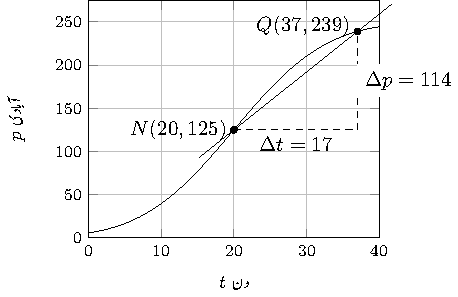
\includegraphics{normalDistributionFlies}
\caption{مکھی کی نمو آبادی}
\label{شکل_حد_مکھی_نمو_آبادی}
\end{minipage}\hfill
\begin{minipage}{0.45\textwidth}
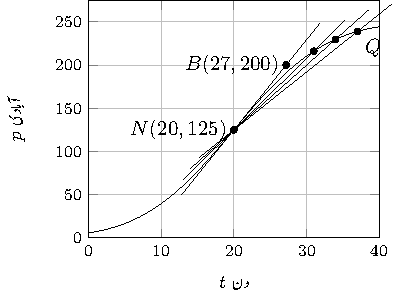
\includegraphics{normalDistributionFliesInstantaneous}
\caption{مکھی کی بیسویں دن نمو آبادی}
\label{شکل_حد_مکھی_نمو_آبادی_بیس}
\end{minipage}%
\end{figure}

حل:\quad
\عددی{20} ویں دن آبادی \عددی{125} تھی جبکہ \عددی{37} ویں دن آبادی \عددی{239} تھی۔ یوں \عددی{37-20=17} دنوں میں آبادی میں \عددی{239-125=114} تبدیل  رونما ہوئی۔یوں شرح تبدیلی درج ذیل ہو گی
\begin{align*}
\frac{\Delta p}{\Delta t}=\frac{114}{17}=6.7 (\text{\RL{مکھیاں فی دن}})
\end{align*}
جو شکل \حوالہ{شکل_حد_مکھی_نمو_آبادی} میں سیکنٹ \عددی{NQ} کی ڈھلوان ہے۔
\انتہا{مثال}
%========================

درج بالا مثال میں \عددی{20} ویں دن سے \عددی{37} ویں دن تک کی اوسط شرح تبدیلی حاصل کی گئی جو ہمیں \عددی{20} ویں دن کی تبدیلی کی شرح کے بارے میں کوئی معلومات فراہم نہیں کرتی ہے۔اس کے لئے ہمیں \عددی{20} ویں دن کے قریب حساب  کرنا ہو گا۔

\ابتدا{مثال}
مثال \حوالہ{مثال_حد_نمو_آبادی_مکھی} میں \عددی{20} ویں دن آبادی میں تبدیلی کی شرح کیا ہے؟\\
حل:\quad
ہمیں نقطہ \عددی{Q} کو نقطہ \عددی{N} کے قریب سے قریب تر کرتے ہوئے شرح حاصل کرنی ہو گی (شکل \حوالہ{شکل_حد_مکھی_نمو_آبادی_بیس})۔یوں درج ذیل حاصل ہوتا ہے۔
\begin{align*}
\begin{array}{ll}
Q&\frac{\Delta p}{\Delta t}\\
\hline
(37,239)&\frac{239-125}{37-20}=6.7\\
(35,230)&\frac{230-125}{35-20}=7\\
(32,216)&\frac{216-125}{32-20}=7.6\\
(27,200)&\frac{200-125}{27-20}=10.7
\end{array}
\end{align*}

جیسے جیسے \عددی{Q} کو بائیں منتقل کیا جائے، خط \عددی{NQ} نقطہ \عددی{N} کے گرد گھڑی کی الٹ رخ گھومتا ہے۔ہم دیکھتے ہیں کہ یہ خط آخر کار \عددی{NB} کو مس کرتا ہے۔اس خط کو دیے گئے منحنی کا \اصطلاح{مماس}\فرہنگ{مماس}\حاشیہب{tangent}\فرہنگ{tangent} کہتے ہیں۔اس طرح ہم توقع کرتے ہیں کہ \عددی{20} ویں دن آبادی کی تبدیلی کی شرح \عددی{10.7} مکھیاں فی دن ہو گی۔
\انتہا{مثال}
%=======================

لمحہ \عددی{t=1} اور لمحہ \عددی{t=2} پر گرتے ہوئے پتھر کی رفتار یا \عددی{20} ویں دن شرح تبدیلی کو \اصطلاح{لمحاتی شرح تبدیلی}\فرہنگ{لمحاتی!شرح تبدیلی}\حاشیہب{instantaneous rates of change}\فرہنگ{instantaneous!rate of change} کہتے ہیں۔جیسا آپ نے دیکھا، ہم اوسط شرح تبدیلی کی تحدیدی قیمت سے لمحاتی شرح تبدیلی حاصل کرتے ہیں۔درج بالا مثال میں ہم نے خط مماس کو بطور خط سیکنٹ کی تحدیدی  صورت پیش کیا۔لمحاتی شرح اور مماس کا گہرا تعلق ہے جو دیگر موضوعات میں بھی پیش آتا ہے۔ اس تعلق کو مزید سمجھنے کی خاطر ہمیں  تحدیدی قیمتوں  کا تعین کرنا سیکھنا ہو گا جنہیں ہم \اصطلاح{حد}\فرہنگ{حد}\حاشیہب{limits}\فرہنگ{limits} کہتے ہیں۔ 

\جزوحصہء{تفاعل کی تحدیدی قیمتیں}
تحدیدی قیمت کی تعریف سے پہلی ایک اور مثال دیکھتے ہیں۔

\ابتدا{مثال}\شناخت{مثال_حد_عجیب_تفاعل_الف}
تفاعل \عددی{f(x)=\tfrac{x^2-1}{x-1}} نقطہ \عددی{x=1} کے قریب کیسا رویہ رکھتا ہے؟\\
حل:\quad
چونکہ صفر سے کسی بھی عدد کو تقسیم نہیں کیا جا سکتا ہے لہٰذا ماسوائے \عددی{x=1} کے، یہ کلیہ تمام حقیقی اعداد کے لئے \عددی{f} تعین کرتا ہے۔کسی بھی \عددی{x\ne 1} کے لئے ہم اس کلیہ کی سادہ صورت حاصل کر سکتے ہیں:
\begin{align*}
f(x)=\frac{x^2-1}{x-1}=\frac{(x-1)(x+1)}{x-1}=x+1\quad\quad (x\ne 1)
\end{align*} 
یوں خط \عددی{y=x+1} جس سے نقطہ \عددی{x=1} یعنی \عددی{(1,2)} خارج کیا گیا ہو اس تفاعل کو ظاہر کرتا ہے۔اس نقطہ کو شکل \حوالہ{شکل_مثال_حد_عجیب_تفاعل_الف} میں بطور سوراخ دکھایا گیا ہے۔اگرچہ نقطہ \عددی{f(1)} غیر معین ہے، ہم \عددی{ x} کی قیمت \عددی{1} کے قریب سے قریب لیتے ہوئے \عددی{f(x)} کی قیمت \عددی{2} کے جتنی قریب چاہیں کر سکتے ہیں۔
\begin{figure}
\centering
\begin{tikzpicture}
\draw[-latex](-1.5,0)--(3,0)node[right]{$x$};
\draw[-latex](0,-0.2)--(0,2.5)node[above]{$y$};
\draw[shorten <=-0.5cm,shorten >=-0.5cm](-1,0)--(1,2);
\foreach \x in {-1,1}{\draw(\x,0)node[below]{$\x$}--++(0,0.1);}
\foreach \y in {1,2}{\draw(0,\y)node[left]{$\y$}--++(0.1,0);}
\draw(1,2)node[ocirc]{};
\draw(0.5,1)node[right]{$y=f(x)=\tfrac{x^2-1}{x-1}$};
\end{tikzpicture}
\caption{شکل برائے مثال \حوالہ{مثال_حد_عجیب_تفاعل_الف}}
\label{شکل_مثال_حد_عجیب_تفاعل_الف}
\end{figure}
%
\begin{align*}
\begin{array}{ll}
\multicolumn{1}{c}{x (\ne 1)}&\multicolumn{1}{c}{f(x)=\tfrac{x^2-1}{x-1}=x+1,\,\, (x\ne 1)}\\
\hline
0.9&1.9\\
1.1&2.1\\
0.99&1.99\\
1.01&2.01\\
0.999&1.999\\
1.001&2.001\\
0.999999&1.999999\\
1.000001&2.000001
\end{array}
\end{align*}

ہم کہتے ہیں کہ \عددی{x} کی قیمت \عددی{1} تک پہنچنے سے \عددی{f(x)} کی قیمت \عددی{2} تک پہنچتی ہے یا \عددی{x} ایک تک پہنچنے سے \عددی{f(x)} تحدیدی قیمت \عددی{2} تک پہنچتی ہے یا حد \عددی{2} تک پہنچتی ہے، جس کو درج ذیل لکھا جاتا ہے۔
\begin{align*}
\lim_{x\to 1} f(x)=2 \quad \text{یا}\quad \lim_{x\to 1} \frac{x^2-1}{x-1}=2
\end{align*}
\عددی{x} کی قیمت \عددی{x_0} تک پہنچنے کو \عددی{x\to x_0} لکھا جاتا ہے۔
\انتہا{مثال}
%====================== 

\ابتدا{تعریف}\موٹا{حد کی غیر رسمی تعریف}\\
فرض کریں کہ \عددی{x_0} کے ارد گرد  ایک کھلے وقفہ پر تفاعل \عددی{f(x)} معین ہے جبکہ عین نقطہ \عددی{x_0} پر \عددی{f(x)} غیر معین ہو سکتا ہے۔ اگر \عددی{x_0} کے کافی قریب \عددی{x} کی  تمام قیمتوں کے لئے \عددی{f(x)} کی قیمتیں \عددی{L} کے کافی قریب پائی جاتی ہوں تب ہم کہتے ہیں کہ \عددی{x} کی قیمت \عددی{x_0} تک پہنچنے سے \عددی{f} کی قیمت \اصطلاح{حد} \عددی{L} تک پہنچتی ہے۔ اس کو ہم درج ذیل لکھتے ہیں۔
\begin{align*}
\lim_{x\to x_0} f(x)=L
\end{align*}
\انتہا{تعریف}
%========================

اس تعریف کو غیر رسمی اس لئے کہا گیا ہے کہ "کافی قریب" کی طرز کے فقرے بہت ٹھیک نہیں ہیں۔خراد پر کام کرنے والے ماہر کے لئے کافی قریب سے مراد \عددی{\SI{10}{\micro\meter}} ہو سکتا ہے جبکہ ماہر فلکیات کے لئے اس کا مطلب چند ہزار نوری سال ہو سکتا ہے۔البتہ یہ تعریف اتنی درست ضرور ہے کہ ہم حد کو پہچان سکیں اور اس کی قیمت حاصل کر سکیں۔ہم حد کی بالکل ٹھیک تعریف جلد پیش کریں گے۔

\ابتدا{مثال}\شناخت{مثال_حد_عجیب_تفاعل_ب}
\عددی{x\to x_0} کی صورت میں \عددی{f} کی حد کی وجودیت \عددی{x_0} پر \عددی{f} کی تعریف کے تابع نہیں ہے۔ شکل \حوالہ{شکل_مثال_حد_عجیب_تفاعل_ب} میں  \عددی{f} کا \عددی{x\to 1} پر حد \عددی{2} ہے اگرچہ \عددی{x=1} پر \عددی{f} غیر معین ہے۔تفاعل \عددی{g} کا \عددی{x\to 1} پر حد \عددی{2} ہے اگرچہ \عددی{x=1} پر \عددی{g(1)=1} ہے۔یوں \عددی{\lim\limits_{x\to 1}g(x)\ne g(1)} ہو گا۔صرف تفاعل \عددی{h} کا \عددی{x\to 1} پر حد اور قیمت دونوں \عددی{2} کے برابر ہیں یعنی \عددی{\lim\limits_{x\to 1} h(x)=h(1)}۔
\begin{figure}
\centering
\begin{subfigure}{0.33\textwidth}
\centering
\begin{tikzpicture}[x=0.75cm]
\draw[-latex](-1.5,0)--(2,0)node[right]{$x$};
\draw[-latex](0,-0.2)--(0,2.5)node[above]{$y$};
\draw[shorten <=-0.5cm,shorten >=-0.5cm](-1,0)--(1,2);
\foreach \x in {-1,1}{\draw(\x,0)node[below]{$\x$}--++(0,0.1);}
\foreach \y in {1,2}{\draw(0,\y)node[left]{$\y$}--++(0.1,0);}
\draw(1,2)node[ocirc]{};
\draw(0,-1)node[font=\footnotesize]{$\begin{aligned}f(x)=\tfrac{x^2-1}{x-1}\end{aligned}$};
\end{tikzpicture}
\caption{}
\end{subfigure}%
\begin{subfigure}{0.33\textwidth}
\centering
\begin{tikzpicture}[x=0.75cm]
\draw[-latex](-1.5,0)--(2,0)node[right]{$x$};
\draw[-latex](0,-0.2)--(0,2.5)node[above]{$y$};
\draw[shorten <=-0.5cm,shorten >=-0.5cm](-1,0)--(1,2);
\foreach \x in {-1,1}{\draw(\x,0)node[below]{$\x$}--++(0,0.1);}
\foreach \y in {1,2}{\draw(0,\y)node[left]{$\y$}--++(0.1,0);}
\draw(1,2)node[ocirc]{};
\draw(1,1)node[circ]{};
\draw(0,-1)node[font=\footnotesize]{$\begin{aligned}g(x)=\begin{cases}\tfrac{x^2-1}{x-1},&x\ne 1\\ 1,&x=1\end{cases}\end{aligned}$};
\end{tikzpicture}
\caption{}
\end{subfigure}%
\begin{subfigure}{0.33\textwidth}
\centering
\begin{tikzpicture}[x=0.75cm]
\draw[-latex](-1.5,0)--(2,0)node[right]{$x$};
\draw[-latex](0,-0.2)--(0,2.5)node[above]{$y$};
\draw[shorten <=-0.5cm,shorten >=-0.5cm](-1,0)--(1,2);
\foreach \x in {-1,1}{\draw(\x,0)node[below]{$\x$}--++(0,0.1);}
\foreach \y in {1,2}{\draw(0,\y)node[left]{$\y$}--++(0.1,0);}
\draw(1,2)node[circ]{};
\draw(0,-1)node[font=\footnotesize]{$\begin{aligned}h(x)=x+1\end{aligned}$};
\end{tikzpicture}
\caption{}
\end{subfigure}%
\caption{$\lim\limits_{x\to 1} f(x)=\lim\limits_{x\to 1}g(x)=\lim\limits_{x\to 1} h(x)=2\quad $}
\label{شکل_مثال_حد_عجیب_تفاعل_ب}
\end{figure}
\انتہا{مثال}
%============================

بعض اوقات \عددی{\lim\limits_{x\to x_0}f(x)} کی قیمت \عددی{f(x_0)} سے حاصل کی جا سکتی ہے۔اس کی مثال تفاعل \عددی{f(x)} ہے جو کثیر رکنی اور تکونیاتی تفاعل کا الجبرائی مجموعہ  ہے اور جہاں \عددی{x_0} پر \عددی{f(x_0)} معین ہو۔

%===============================
\ابتدا{مثال}\شناخت{مثال_حد_عجیب_تفاعل_پ}
\begin{enumerate}[a.]
\item
$\lim\limits_{x\to 2} (4)=4$
\item
$\lim\limits_{x\to 13}(4)=4$
\item
$\lim\limits_{x\to 3} x=3$
\item
$\lim\limits_{x\to 2} (5x-3)=10-3=7$
\item
$\lim\limits_{x\to -2}\frac{3x+4}{x+5}=\frac{-6+4}{-2+5}=-\frac{2}{3}$
\end{enumerate}
\انتہا{مثال}
%================================
\ابتدا{مثال}\شناخت{مثال_حد_مماثل_تفاعل}
\begin{enumerate}[a.]
\item
اگر \عددی{f} مماثلی تفاعل \عددی{f(x)=x} ہو تب \عددی{x_0} کے کسی بھی قیمت کے لئے  درج ذیل ہو گا (شکل \حوالہ{شکل_مثال_حد_عجیب_تفاعل_پ}-ل)۔
\begin{align*}
\lim\limits_{x\to x_0} f(x)=\lim\limits_{x\to x_0} x=x_0
\end{align*}
\item
اگر \عددی{f} مستقل تفاعل \عددی{f(x)=k} ہو (جہاں \عددی{k} مستقل ہے) تب \عددی{x_0} کے کسی بھی قیمت کے لئے درج ذیل ہو گا (شکل \حوالہ{شکل_مثال_حد_عجیب_تفاعل_پ}-ب)۔
\begin{align*}
\lim\limits_{x\to x_0} f(x)=\lim\limits_{x\to x_0} k=k
\end{align*} 
\end{enumerate}
%
\begin{figure}
\centering
\begin{subfigure}{0.5\textwidth}
\centering
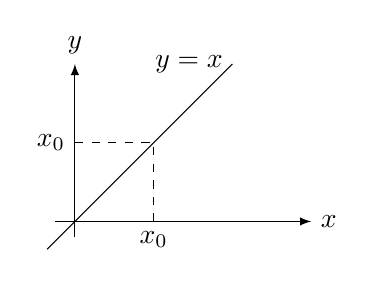
\begin{tikzpicture}
\draw[-latex](-0.25,0)--(3,0)node[right]{$x$};
\draw[-latex](0,-0.2)--(0,2)node[above]{$y$};
\draw[shorten <=-0.5cm](0,0)--(2,2)node[pos=1,left]{$y=x$};
\draw[dashed] (0,1)node[left]{$x_0$}--(1,1)--(1,0)node[below]{$x_0$};
\end{tikzpicture}
\caption{مماثل تفاعل}
\end{subfigure}%
\begin{subfigure}{0.5\textwidth}
\centering
\begin{tikzpicture}
\draw[-latex](-0.25,0)--(3,0)node[right]{$x$};
\draw[-latex](0,-0.2)--(0,2)node[above]{$y$};
\draw(-0.25,1)--(3,1)node[pos=0.9,above]{$y=k$};
\draw(0,1)node[circ]{}node[above left]{$k$};
\draw[dashed](1,0)node[below]{$x_0$}--(1,1)node[circ]{};
\draw(0,0)node[below left]{$M$};
\end{tikzpicture}
\caption{مستقل تفاعل}
\end{subfigure}%
\caption{اشکال برائے مثال \حوالہ{مثال_حد_عجیب_تفاعل_پ}}
\label{شکل_مثال_حد_عجیب_تفاعل_پ}
\end{figure}
\انتہا{مثال}
%==================================
\ابتدا{مثال}\شناخت{مثال_حد_عجیب_تفاعل_ت} \ترچھا{عین ممکن ہے کہ تفاعل کے دائرہ کار میں تفاعل کا حد نہ پایا جاتا ہو۔}\\ 
درج ذیل تفاعل کا \عددی{x\to 0} پر رویہ کیسا ہو گا؟
\begin{enumerate}[a.]
\item
$U(x)=\begin{cases}0,&x<0\\ 1,&x\ge 0  \end{cases}$
\item
$g(x)=\begin{cases} \tfrac{1}{x},&x\ne 0\\ 0,&x=0 \end{cases}$
\item
$f(x)=\begin{cases}0,&x\le 0\\ \sin \tfrac{1}{x},&x>0  \end{cases}$
\end{enumerate}
%

حل:\quad
\begin{enumerate}[a.]
\item
اکائی سیڑھی تفاعل \عددی{U(x)} کا \عددی{x\to 0} پر کوئی حد نہیں پایا جاتا ہے چونکہ اس نقطہ پر تفاعل کی چھلانگ پائی جاتی ہے۔\عددی{0} کے کافی قریب \عددی{x} کی منفی قیمتوں کے لئے \عددی{U} کی قیمت \عددی{0} ہے جبکہ \عددی{0} کے کافی  قریب  \عددی{x}  کی مثبت قیمتوں کے لئے \عددی{U} کی قیمت \عددی{1} ہے۔یوں \عددی{0} کے قریب پہنچنے سے \عددی{U} کی منفرد قیمت نہیں پائی جاتی ہے (شکل \حوالہ{شکل_مثال_حد_عجیب_تفاعل_ت}-ا)۔
\item
\عددی{x=0} کے کافی قریب تفاعل کی قیمت بے قابو بڑھتی ہے اور کسی ایک منفرد قیمت تک پہنچنے کی کوشش نہیں کرتی ہے (شکل \حوالہ{شکل_مثال_حد_عجیب_تفاعل_ت}-ب)۔
\item
\عددی{x=0} کے کافی قریب تفاعل بہت زیادہ ارتعاش کرتا ہے۔اس کی قیمت کسی مخصوص قیمت تک پہنچنے کی کوشش نہیں کرتی ہے (شکل \حوالہ{شکل_مثال_حد_عجیب_تفاعل_ت}-ج)۔ 
\end{enumerate}
%
\begin{figure}
\centering
\begin{subfigure}{0.33\textwidth}
\centering
\begin{tikzpicture}
\begin{axis}[clip=false,small,axis lines=middle,width=4cm,xtick={\empty},ytick={1},xlabel={$x$},ylabel={$y$},xlabel style={at={(current axis.right of origin)},anchor={west}},ylabel style={at={(current axis.above origin)},anchor=south},ymin=-0.5,ymax=2]
\addplot[domain=-2:0]{0};
\addplot[domain=0:2]{1};
\draw(axis cs:0,0)node[ocirc]{};
\draw(axis cs:0,1)node[circ]{};
\draw(axis cs:0,1)node[above right,font=\footnotesize]{$\begin{aligned}y=\begin{cases}0,&x<0\\ 1,&x\ge 1\end{cases}\end{aligned}$};
\end{axis}
\end{tikzpicture}
\caption{اکائی سیڑھی تفاعل $U(x)\,\,$}
\end{subfigure}%
\begin{subfigure}{0.33\textwidth}
\centering
\begin{tikzpicture}
\begin{axis}[clip=false,small,axis lines=middle,width=4cm,xtick={\empty},ytick={\empty},xlabel={$x$},ylabel={$y$},xlabel style={at={(current axis.right of origin)},anchor={west}},ylabel style={at={(current axis.above origin)},anchor=south}]
\addplot[domain=-4:-0.3]{1/x};
\addplot[domain=0.3:4]{1/x};
\draw(axis cs:0,0)node[circ]{}node[below right]{$0$};
\draw(axis cs:0.4,1)node[above right,font=\footnotesize]{$\begin{aligned}y=\begin{cases}\tfrac{1}{x},&x\ne 0\\ 0,&x=0\end{cases}\end{aligned}$};
\end{axis}
\end{tikzpicture}
\caption{$g(x)$}
\end{subfigure}%
\begin{subfigure}{0.33\textwidth}
\centering
\begin{tikzpicture}
\begin{axis}[clip=false,small,axis lines=middle,width=4cm,xtick={\empty},ytick={-1,1},xlabel={$x$},ylabel={$y$},xlabel style={at={(current axis.right of origin)},anchor={west}},ylabel style={at={(current axis.above origin)},anchor=south},ymin=-1.2,ymax=1.2]
\addplot[domain=-0.2:0]{0}node[circ]{};
\addplot[domain=0.052:0.08,samples=100]{sin(180/(pi*x)};
\addplot[domain=0.08:0.5,samples=100]{sin(180/(pi*x)};
\draw(axis cs:0,0)node[circ]{}node[below left]{$0$};
\draw(axis cs:0.2,-0.75)node[right,font=\footnotesize]{$\begin{aligned}y=\begin{cases}0 ,&x\le  0\\  \sin \tfrac{1}{x},&x>0\end{cases}\end{aligned}$};
\end{axis}
\end{tikzpicture}
\caption{$f(x)$}
\end{subfigure}%
\caption{اشکال برائے مثال \حوالہ{مثال_حد_عجیب_تفاعل_ت}}
\label{شکل_مثال_حد_عجیب_تفاعل_ت}
\end{figure}
\انتہا{مثال}
%=================================

\حصہء{سوالات \حوالہ{حصہ_حد_تبدیلی_کی_شرح_اور_حد}}

\موٹا{ترسیم سے حد}

\ابتدا{سوال}\شناخت{سوال_حد_ترسیم_سے_حد_الف}
شکل \حوالہ{شکل_سوال_حد_ترسیم_سے_حد_الف}-ا میں دی گئی ترسیم سے درج ذیل حد تلاش کریں یا حد نا ہونے کی وجہ بیان کریں۔
\begin{multicols}{3}
\begin{enumerate}[a.]
\item
$\lim\limits_{x\to 1} g(x)$
\item
$\lim\limits_{x\to 2} g(x)$
\item
$\lim\limits_{x\to 3}g(x)$
\end{enumerate}
\end{multicols}
%
\begin{figure}
\centering
\begin{subfigure}{0.5\textwidth}
\centering
\begin{tikzpicture}
\draw[-latex](-0.25,0)--(4,0)node[right]{$x$};
\draw[-latex](0,-0.2)--(0,1.5)node[above]{$y$};
\draw[dashed](0,1)node[left]{$1$}--(3,1)node[solid,circ]{};
\draw(-0.2,-0.2)--(1,1)node[ocirc]{};
\draw(1,0)node[circ]{}--(2,1)node[circ]{}node[above,yshift={2mm}]{$y=g(x)$}--(3,0)node[ocirc]{}--(3.9,0.9);
\foreach \x in {1,2,3}{\draw(\x,0)node[below]{$\x$}--++(0,0.1);}
\end{tikzpicture}
\caption{}
\end{subfigure}%
\begin{subfigure}{0.5\textwidth}
\centering
\begin{tikzpicture}
\draw[-latex](-3,0)--(2,0)node[right]{$t$};
\draw[-latex](0,-1.25)--(0,1.5)node[above]{$s$};
\draw(-3,-1)--(-2,0)node[ocirc]{}node[above,yshift={2mm}]{$s=f(t)$}--(-1,-1)node[circ]{}--(0,-1)node[ocirc]{}node[right]{$-1$};
\foreach \x in {-2,-1,1}{\draw(\x,0)node[below]{$\x$}--++(0,0.1);}
\draw(0,0)node[circ]{}node[below left]{$0$};
\draw(0,1)node[ocirc]{}node[left]{$1$}--(2,1);
\end{tikzpicture}
\caption{}
\end{subfigure}%
\caption{اشکال برائے سوال \حوالہ{سوال_حد_ترسیم_سے_حد_الف} اور سوال \حوالہ{سوال_حد_ترسیم_سے_حد_ب}}
\label{شکل_سوال_حد_ترسیم_سے_حد_الف}
\end{figure}

جواب: (ا) موجود نہیں ہے۔جیسے جیسے \عددی{x} دائیں سے \عددی{1} کے نزدیک تر ہوتا  ہے ویسے ویسے \عددی{g(x)} کی قیمت \عددی{0} کے نزدیک تر ہوتی ہے۔جیسے جیسے \عددی{x} بائیں سے \عددی{1} کے نزدیک تر ہوتا ہے  ویسے ویسے \عددی{g(x)} کی قیمت \عددی{1} کے نزدیک تر ہوتی ہے۔یوں \عددی{x} کی قیمت \عددی{1} کے نزدیک تر ہونے سے \عددی{L} کی یکتا قیمت کے نزدیک تر \عددی{g(x)} نہیں پہنچتا ہے۔ (ب) \عددی{1} (ج) \عددی{0} 
\انتہا{سوال}
%=====================
\ابتدا{سوال}\شناخت{سوال_حد_ترسیم_سے_حد_ب}
شکل \حوالہ{شکل_سوال_حد_ترسیم_سے_حد_الف}-ب میں دی گئی ترسیم سے درج ذیل حد تلاش کریں یا حد نا ہونے کی وجہ بیان کریں۔
\begin{multicols}{3}
\begin{enumerate}[a.]
\item
$\lim\limits_{t\to -2}f(t)$
\item
$\lim\limits_{t\to -1}f(t)$
\item
$\lim\limits_{t\to 0}f(t)$
\end{enumerate}
\end{multicols}
\انتہا{سوال}
%======================
\ابتدا{سوال}\شناخت{سوال_حد_ترسیم_سے_حد_پ}
تفاعل \عددی{y=f(x)}  (شکل \حوالہ{سوال_حد_ترسیم_سے_حد_پ}-ا) کے لئے درج ذیل فقروں میں سے کون سے درست ہیں؟
\begin{multicols}{3}
\begin{enumerate}[a.]
\item
$\lim\limits_{x\to 0}f(x)$ موجود ہے\\
\item
$\lim\limits_{x\to 0}f(x)=0$
\item
$\lim\limits_{x\to 0}f(x)=1$
\item
$\lim\limits_{x\to 1}f(x)=1$
\item
$\lim\limits_{x\to 1}f(x)=0$
\item
$\lim\limits_{x\to x_ 0}f(x)$
وقفہ \عددی{(-1,1)} میں ہر نقطہ \عددی{x_0} پر موجود ہے
\end{enumerate}
\end{multicols}
%
\begin{figure}
\centering
\begin{subfigure}{0.5\textwidth}
\centering
\begin{tikzpicture}
\draw[-latex](-1.2,0)--(3,0)node[right]{$x$};
\draw[-latex](0,-1.2)--(0,1.5)node[above]{$y$};
\draw(-1,-1)node[circ]{}--(0,0)node[ocirc]{}--(1,-1)node[ocirc]{} (1,0)node[circ]{}--(2,1)node[circ]{};
\draw(0,1)node[circ]{}node[left]{$1$}--++(0.1,0);
\foreach \x in {-1,1,2}{\draw(\x,0)node[below]{$\x$}--++(0,0.1);} 
\draw(0,-1)node[left]{$-1$}--++(0.1,0);
\draw(0.5,1.25)node[right]{$y=f(x)$};
\end{tikzpicture}
\caption{}
\end{subfigure}%
\begin{subfigure}{0.5\textwidth}
\centering
\begin{tikzpicture}[]
\draw[-latex](-1.2,0)--(3.5,0)node[right]{$x$};
\draw[-latex](0,-2.2)--(0,1.5)node[above]{$y$};
\foreach \x in {-1,1,2,3}{\draw(\x,0)node[below]{$\x$}--++(0,0.1);} 
\foreach \y in {-2,-1,1}{\draw(0,\y)node[left]{$\y$}--++(0.1,0);}
\draw(-1,-1)node[circ]{}--(0,0)node[circ]{};
\draw[domain=0:1] plot ({\x},{-2*\x*\x});
\draw([shift={(0:1)}]2,0) arc (0:180:1);
\draw(1,0)node[circ]{} (2,0)node[circ]{} (3,0)node[circ]{} (2,1)node[ocirc]{}node[above]{$y=f(x)$};
\end{tikzpicture}
\caption{}
\end{subfigure}%
\caption{اشکال برائے سوال \حوالہ{سوال_حد_ترسیم_سے_حد_پ} اور سوال \حوالہ{سوال_حد_ترسیم_سے_حد_ت}}
\label{شکل_سوال_حد_ترسیم_سے_حد_پ}
\end{figure}

جواب: (ا) درست (ب) درست (ج) غلط (د) غلط  (ہ) غلط (و) درست
\انتہا{سوال}
%============================
\ابتدا{سوال}\شناخت{سوال_حد_ترسیم_سے_حد_ت}
تفاعل \عددی{y=f(x)} (شکل \حوالہ{سوال_حد_ترسیم_سے_حد_پ}-ب)  کے لئے درج ذیل فقروں میں سے کون سے درست ہیں؟
\begin{multicols}{3}
\begin{enumerate}[a.]
\item
$\lim\limits_{x\to 2} f(x)$
موجود نہیں ہے
\item
$\lim\limits_{x\to 2}f(x)=2$
\item
$\lim\limits_{x\to 1}f(x)$
موجود نہیں ہے
\item
$\lim\limits_{x\to x_0}f(x)$
وقفہ \عددی{(-1,1)} میں ہر نقطہ \عددی{x_0} پر موجود ہے۔
\item
$\lim\limits_{x\to x_0}f(x)$
وقفہ \عددی{(1,3)} میں ہر نقطہ \عددی{x_0} پر موجود ہے۔
\end{enumerate}
\end{multicols}
\انتہا{سوال}
%======================

\موٹا{وجودیت اور حد}

سوال \حوالہ{سوال_حد_غیر_موجود_الف} اور سوال \حوالہ{سوال_حد_غیر_موجود_ب} میں حد کی غیر موجودگی کی وجہ بیان کریں۔

\ابتدا{سوال}\شناخت{سوال_حد_غیر_موجود_الف}
$\lim\limits_{x \to 0}\tfrac{x}{\abs{x}}$\\
جواب: جیسے جیسے \عددی{x} بائیں سے \عددی{1} کے نزدیک تر ہوتا ہے ویسے ویسے \عددی{\tfrac{x}{\abs{x}}} کی قیمت \عددی{-1} کے نزدیک تر ہوتی ہے ۔جب \عددی{x} دائیں سے \عددی{1} کے نزدیک تر ہوتا ہے ویسے \عددی{\tfrac{x}{\abs{x}}} کی قیمت \عددی{-1} کے نزدیک تر ہوتی ہے۔یوں \عددی{x} کا \عددی{1} کے نزدیک تر ہونے سے  \عددی{\tfrac{x}{\abs{x}}} کسی یکتا قیمت کے نزدیک تر نہیں ہوتی ہے۔ 
\انتہا{سوال}
%======================
\ابتدا{سوال}\شناخت{سوال_حد_غیر_موجود_ب}
$\lim\limits_{x \to 1}\tfrac{1}{x-1}$
\انتہا{سوال}
%======================
\ابتدا{سوال}
فرض کریں کہ ماسوائے نقطہ \عددی{x=x_0} تفاعل \عددی{f(x)} تمام حقیقی \عددی{x} کے لئے معین ہے۔کیا \عددی{\lim\limits_{x\to x_0}f(x)} کی وجودیت کی وجودیت کے بارے میں کچھ کہنا ممکن ہے؟ اپنے جواب کی وجہ بیان کریں۔ 
\انتہا{سوال}
%======================
\ابتدا{سوال}
فرض کریں کہ  تفاعل \عددی{f(x)} وقفہ \عددی{[-1,1]} میں تمام  \عددی{x} کے لئے معین ہے۔کیا \عددی{\lim\limits_{x\to 0}f(x)} کے بارے میں کچھ کہنا ممکن ہے؟ اپنے جواب کی وجہ بیان کریں۔ 
\انتہا{سوال}
%======================
\ابتدا{سوال}
اگر \عددی{\lim\limits_{x\to 1}f(x)=5} ہو تب کیا \عددی{x=1} پر \عددی{f} کا معین ہونا لازم ہے؟اگر معین ہونا لازم ہو تب کیا \عددی{f(1)=5} ہونا لازم ہے؟ کیا \عددی{x=1} پر ہم \عددی{f} کی قیمت کے بارے میں کچھ کہہ سکتے ہیں؟ وضاحت کریں۔
\انتہا{سوال}
%======================
\ابتدا{سوال}
اگر \عددی{f(1)=5} ہو تب کیا \عددی{\lim\limits_{x\to 1}f(x)} لازماً موجود ہو گا؟ اگر ایسا ہو تب کیا \عددی{\lim\limits_{x\to 1}f(x)=5} لازماً ہو گا؟ کیا ہم  \عددی{\lim\limits_{x\to 1}f(x)} کے بارے میں کوئی نتیجہ اخذ کر سکتے ہیں؟ وضاحت کریں۔
\انتہا{سوال}
%======================

\موٹا{کیلکولیٹر اور کمپیوٹر کا استعمال}

\ابتدا{سوال}
\عددی{f(x)=\tfrac{x^2-9}{x+3}} لیں۔
\begin{enumerate}[a.]
\item
\عددی{f} کی قیمتوں کا جدول نقاط \عددی{x=-3.1,-3.01,-3.001,\cdots} پر وہاں تک تلاش کریں جہاں تک آپ کا کیلکولیٹر جواب حاصل کر سکتا ہو۔اس جدول سے \عددی{\lim\limits_{x\to -3}f(x)} کی اندازاً قیمت حاصل کریں۔اس کے برعکس نقاط \عددی{x=-2.9,-2.99,\cdots} پر \عددی{f} کی قیمتیں استعمال کرتے ہوئے نتیجہ کیا ہو گا؟
\item
تفاعل کو \عددی{x_0=-3} کے قریب ترسیم کریں۔ ترسیم پر \عددی{x\to -3} کے لئے \عددی{y} کی قیمت دیکھ کر  گزشتہ جزو کے نتائج کی تصدیق کریں۔ 
\item
\عددی{\lim\limits_{x\to -3}f(x)} کو الجبرائی طریقہ سے اخذ کریں۔
\end{enumerate}

جواب: (ا) 
\begin{align*}
\begin{array}{|c|c|c|c|c|c|c|}
\hline
x&-3.1&-3.01&-3.001&-3.0001&-3.00001&-3.000001\\
f(x)&-6.1&-6.01&-6.001&-6.0001&-6.00001&-6.000001\\
\hline
\end{array}\\
\begin{array}{|c|c|c|c|c|c|c|}
\hline
x&-2.9&-2.99&-2.999&-2.9999&-2.99999&-2.999999\\
f(x)&-5.9&-5.99&-5.999&-5.9999&-5.99999&-5.999999\\
\hline
\end{array}
\end{align*}
(ج) 
$\lim_{x\to -3} f(x)=-6$ 
\انتہا{سوال}
%=========================
\ابتدا{سوال}
\عددی{g(x)=\tfrac{x^2-2}{x-\sqrt{2}}} لیں۔
\begin{enumerate}[a.]
\item
\عددی{\sqrt{2}} کی تخمینی قیمتوں \عددی{x=1.4,1.41,1.414,\cdots} پر تفاعل کی قیمتوں کے جدول سے \عددی{\lim\limits_{x\to \sqrt{2}}g(x)}  کی اندازاً قیمت حاصل کریں۔
\item
نقطہ \عددی{x_0=\sqrt{2}} کے قریب تفاعل ترسیم کریں۔\عددی{x\to \sqrt{2}} کے لئے ترسیم سے \عددی{y} کی قیمت دیکھ کر گزشتہ جزو کی جواب کا تصدیق کریں۔
\item
\عددی{\lim\limits_{x\to\sqrt{2}}g(x)} کو الجبرائی طور پر حاصل کریں۔
\end{enumerate}
\انتہا{سوال}
%====================
\ابتدا{سوال}
\عددی{G(x)=\tfrac{x+6}{x^2+4x-12}} لیں۔
\begin{enumerate}[a.]
\item
نقاط \عددی{x=-5.9,-5.99,-5.999,\cdots} پر \عددی{G} کی قیمتوں کا جدول بنا کر \عددی{\lim\limits_{x\to -6}G(x)} کی اندازاً قیمت حاصل کریں۔ اس کے برعکس \عددی{x=-6.1,-6.01,-6.001,\cdots} پر \عددی{G} کی قیمتیں استعمال کرتے ہوئے کیا نتیجہ حاصل ہو گا؟
\item
\عددی{G} کو \عددی{x_0=6} کے قریبی نقطوں پر تقسیم کرتے ہوئے \عددی{x\to -6} کے لئے \عددی{G} کی قیمت دیکھ کر گزشتہ جزو کے نتائج کی تصدیق کریں۔
\item
\عددی{\lim\limits_{x\to -6}G(x)} کو الجبرائی طریقہ سے حاصل کریں۔
\end{enumerate}
جواب: (ا)
\begin{align*}
\begin{array}{|c|c|c|c|c|c|c|}
\hline
x&-5.9&-5.99&-5.999&-5.9999&-5.99999&-5.999999\\
G(x)&-0.126582&-0.1251564&-0.1250156&-0.1250015&-0.1250001&-0.1250000\\
\hline
\end{array}\\
\begin{array}{|c|c|c|c|c|c|c|}
\hline
x&-6.1&-6.01&-6.001&-6.0001&-6.00001&-6.000001\\
G(x)&-0.123456&-0.124843&-0.124984&-0.124998&-0.124999&-0.124999\\
\hline
\end{array}
\end{align*}
(ج)
$\lim_{x\to -6} G(x)=-\tfrac{1}{8}=-0.125$ 
\انتہا{سوال}
%======================
\ابتدا{سوال}
\عددی{h(x)=\tfrac{x^2-2x-3}{x^2-4x+3}} لیں۔
\begin{enumerate}[a.]
\item
نقاط \عددی{x=2.9, 2.99, 2.999,\cdots} پر \عددی{h} کی قیمتوں کے جدول سے \عددی{\lim\limits_{x\to 3}h(x)} کی اندازاً قیمت تلاش کریں۔اس کے برعکس \عددی{x=3.1,3.01,3.001,\cdots} پر \عددی{h} کی قیمتیں لیتے ہوئے نتیجہ کیا ہو گا؟
\item
\عددی{x_0=3} کے قریب \عددی{h} ترسیم کر کے \عددی{x\to 3} کے لئے \عددی{h(x)} کی قیمت دیکھ کر گزشتہ جزو کے نتائج کی تصدیق کریں۔
\item
\عددی{\lim\limits_{x\to 3}h(x)} کو الجبرائی طریقہ سے حاصل کریں۔
\end{enumerate}
\انتہا{سوال}
%=====================
\ابتدا{سوال}
\عددی{f(x)=\tfrac{x^2-1}{\abs{x}-1}} لیں۔
\begin{enumerate}[a.]
\item
\عددی{f} کی قیمتوں کا جدول \عددی{x} کی ان قیمتوں کے لئے بنائیں جو \عددی{x_0=-1} تک نیچے سے اور اوپر سے پہنچنے کی کوشش کرتی ہیں۔اس جدول سے \عددی{\lim\limits_{x\to-1}f(x)} کی اندازاً قیمت تلاش کریں۔  
\item
\عددی{x_0=-1} کے قریب \عددی{f} ترسیم کریں۔ترسیم سے \عددی{x\to -1} کے لئے \عددی{y} کی قیمتیں دیکھ کر گزشتہ جزو کے نتائج کی تصدیق کریں۔
\item
\عددی{\lim\limits_{x\to -1}f(x)} کو الجبرائی طریقہ سے حاصل کریں۔
\end{enumerate}
جواب: (ا)
\begin{align*}
\begin{array}{|c|c|c|c|c|c|c|}
\hline
x&-1.1&-1.01&-1.001&-1.0001&-1.00001&-1.000001\\
f(x)&2.1&2.01&2.001&2.0001&2.00001&2.000001\\
\hline
\end{array}\\
\begin{array}{|c|c|c|c|c|c|c|}
x&-0.9&-0.99&-0.999&-0.9999&-0.99999&-0.999999\\
f(x)&1.9&1.99&1.999&1.9999&1.99999&1.999999\\
\hline
\end{array}
\end{align*}
(ج)
$\lim_{x\to -1} f(x)=2$
\انتہا{سوال}
%========================
\ابتدا{سوال}
\عددی{F(x)=\tfrac{x^2+3x+2}{2-\abs{x}}} لیں۔
\begin{enumerate}[a.]
\item
\عددی{F} کی قیمتوں کا جدول \عددی{x} کی ان قیمتوں کے لئے بنائیں جو \عددی{x_0=-2} تک نیچے سے اور اوپر سے پہنچنے کی کوشش کرتی ہیں۔اس جدول سے
 \عددی{\lim\limits_{x\to-2}F(x)} کی اندازاً قیمت تلاش کریں۔  
\item
\عددی{x_0=-2} کے قریب \عددی{F} ترسیم کریں۔ترسیم سے \عددی{x\to -2} کے لئے \عددی{y} کی قیمتیں دیکھ کر گزشتہ جزو کے نتائج کی تصدیق کریں۔
\item
\عددی{\lim\limits_{x\to -2}F(x)} کو الجبرائی طریقہ سے حاصل کریں۔
\end{enumerate}
\انتہا{سوال}
%========================
\ابتدا{سوال}
\عددی{g(\theta)=\tfrac{\sin\theta}{\theta}} لیں۔
\begin{enumerate}[a.]
\item
\عددی{g} کی قیمتوں کا جدول \عددی{\theta} کی ان قیمتوں کے لئے بنائیں جو \عددی{\theta_0=0} تک نیچے سے اور اوپر سے پہنچنے کی کوشش کرتی ہیں۔اس جدول سے
 \عددی{\lim\limits_{x\to 0}g(\theta)} کی اندازاً قیمت تلاش کریں۔  
\item
\عددی{\theta_0=0} کے قریب \عددی{g} ترسیم کریں۔ترسیم سے گزشتہ جزو کے نتائج کی تصدیق کریں۔
\end{enumerate}
جواب:(ا)
\begin{align*}
\begin{array}{|c|c|c|c|c|c|c|}
\hline
\theta&0.1&0.01&0.001&0.0001&0.00001&0.000001\\
g(\theta)&0.998334&0.999983&0.999999&0.999999&0.999999&0.999999\\
\hline
\end{array}\\
\begin{array}{|c|c|c|c|c|c|c|}
\hline
\theta&-0.1&-0.01&-0.001&-0.0001&-0.00001&-0.000001\\
g(\theta)&0.998334&0.999983&0.999999&0.999999&0.999999&0.999999\\
\hline
\end{array}
\end{align*}
(ج)
$\lim_{\theta \to 0} g(\theta)=1$
\انتہا{سوال}
%========================
\ابتدا{سوال}
\عددی{G(t)=\tfrac{1-\cos t}{t^2}} لیں۔
\begin{enumerate}[a.]
\item
\عددی{G} کی قیمتوں کا جدول \عددی{t} کی ان قیمتوں کے لئے بنائیں جو \عددی{t_0=0} تک نیچے سے اور اوپر سے پہنچنے کی کوشش کرتی ہیں۔اس جدول سے
 \عددی{\lim\limits_{t\to 0}G(t)} کی اندازاً قیمت تلاش کریں۔  
\item
\عددی{t_0=0} کے قریب \عددی{G} ترسیم کریں۔ترسیم سے گزشتہ جزو کے نتائج کی تصدیق کریں۔
\end{enumerate}
\انتہا{سوال}
%===================
\ابتدا{سوال}
\عددی{f(x)=x^{\tfrac{1}{1-x}}} لیں۔
\begin{enumerate}[a.]
\item
\عددی{f} کی قیمتوں کا جدول \عددی{x} کی ان قیمتوں کے لئے بنائیں جو \عددی{x_0=1} تک نیچے سے اور اوپر سے پہنچنے کی کوشش کرتی ہیں۔کیا \عددی{x} کی قیمت \عددی{x\to 1} تک پہنچنے سے \عددی{f} کا تحدیدی نقطہ پایا جاتا ہے؟ اگر تحدیدی نقطہ پایا جاتا ہو، اس کا تلاش کریں۔اگر نہیں پایا جاتا ہو تب وجہ بیان کریں۔
\item
\عددی{x_0=1} کے قریب \عددی{f} ترسیم کریں۔ترسیم سے گزشتہ جزو کے نتائج کی تصدیق کریں۔
\end{enumerate}
جواب: (ا)
\begin{align*}
\begin{array}{|c|c|c|c|c|c|c|}
\hline
x&0.9&0.99&0.999&0.9999&0.99999&0.999999\\
f(x)&0.348678&0.366032&0.367695&0.367861&0.367877&0.367879\\
\hline
\end{array}\\
\begin{array}{|c|c|c|c|c|c|c|}
\hline
x&1.1&1.01&1.001&1.0001&1.00001&1.000001\\
f(x)&0.385543&0.369711&0.368063&0.367897&0.367881&0.367878\\
\hline
\end{array}
\end{align*}
(ج)
$\lim_{x\to 1}f(x)\approx 0.36788$
\انتہا{سوال}
%=============================
\ابتدا{سوال}
\عددی{f(x)=\tfrac{3^x-1}{x}} لیں۔
\begin{enumerate}[a.]
\item
\عددی{f} کی قیمتوں کا جدول \عددی{x} کی ان قیمتوں کے لئے بنائیں جو \عددی{x_0=0} تک نیچے سے اور اوپر سے پہنچنے کی کوشش کرتی ہیں۔کیا
 \عددی{x} کی قیمت \عددی{x\to 0} تک پہنچنے سے \عددی{f} کا تحدیدی نقطہ پایا جاتا ہے؟ اگر تحدیدی نقطہ پایا جاتا ہو، اس کا تلاش کریں۔اگر نہیں پایا جاتا ہو تب وجہ بیان کریں۔
\item
\عددی{x_0=0} کے قریب \عددی{f} ترسیم کریں۔ترسیم سے گزشتہ جزو کے نتائج کی تصدیق کریں۔
\end{enumerate}
\انتہا{سوال}
%=============================
\موٹا{متغیر کی تحدیدی قیمت پر کرتے ہوئے حد کا تعین}

سوال \حوالہ{سوال_حد_پر_الف} تا سوال \حوالہ{سوال_حد_پر_ب} میں متغیر \عددی{x} کی تحدیدی قیمت کو تفاعل میں پر کرتے ہوئے تفاعل کی حد تلاش کریں۔

\ابتدا{سوال}\شناخت{سوال_حد_پر_الف}
$\lim\limits_{x\to 2} 2x$\\
جواب:\quad
$4$
\انتہا{سوال}
%========================
\ابتدا{سوال}
$\lim\limits_{x\to 0} 2x$
\انتہا{سوال}
%========================
\ابتدا{سوال}
$\lim\limits_{x\to \tfrac{1}{3}} (3x-1)$\\
جواب:\quad
$0$
\انتہا{سوال}
%========================
\ابتدا{سوال}
$\lim\limits_{x\to 1} -\tfrac{1}{3x-1}$
\انتہا{سوال}
%========================
\ابتدا{سوال}
$\lim\limits_{x\to -1} 3x(2x-1)$\\
جواب:\quad
$9$
\انتہا{سوال}
%========================
\ابتدا{سوال}
$\lim\limits_{x\to -1} \tfrac{3x^2}{2x-1}$
\انتہا{سوال}
%========================
\ابتدا{سوال}
$\lim\limits_{x\to \tfrac{\pi}{2}} x\sin x$\\
جواب:\quad
$\tfrac{\pi}{2}$
\انتہا{سوال}
%========================
\ابتدا{سوال}\شناخت{سوال_حد_پر_ب}
$\lim\limits_{x\to \pi} \tfrac{\cos x}{1-\pi}$
\انتہا{سوال}
%========================

\موٹا{اوسط شرح تبدیلی}

سوال \حوالہ{سوال_حد_اوسط_تبدیلی_شرح_الف} تا سوال \حوالہ{سوال_حد_اوسط_تبدیلی_شرح_ب} میں دیے وقفہ پر تفاعل کی اوسط شرح تبدیلی تلاش کریں۔

\ابتدا{سوال}\شناخت{سوال_حد_اوسط_تبدیلی_شرح_الف}
\عددی{f(x)=x^3+1}؛ (الف) \عددی{[2,3]}، (ب) \عددی{[-1,1]}\\
جواب:\quad (ا)
$19$ 
\quad
(ب)\quad
$1$
\انتہا{سوال}
%======================
\ابتدا{سوال}
\عددی{g(x)=x^2}؛ (الف) \عددی{[-1,1]}، (ب) \عددی{[-2,0]}
\انتہا{سوال}
%======================
\ابتدا{سوال}
\عددی{h(t)=\cos t}؛ (الف) \عددی{[\tfrac{\pi}{4},\tfrac{3\pi}{4}]}، (ب) \عددی{[\tfrac{\pi}{6},\tfrac{\pi}{2}]}\\
جواب:\quad (ا) \عددی{-\tfrac{4}{\pi}} 
\quad
(ب) \عددی{-\tfrac{3\sqrt{3}}{\pi}}
\انتہا{سوال}
%======================
\ابتدا{سوال}
\عددی{g(t)=2+\cos t}؛ (الف) \عددی{[0,\pi]}، (ب) \عددی{[-\pi,\pi]}
\انتہا{سوال}
%======================
\ابتدا{سوال}
\عددی{R(\theta)=\sqrt{4\theta+1}}؛  \عددی{[0,2]}\\
جواب:\quad
$1$
\انتہا{سوال}
%======================
\ابتدا{سوال}\شناخت{سوال_حد_اوسط_تبدیلی_شرح_ب}
\عددی{P(\theta)=\theta^3-4\theta^2+5\theta}؛  \عددی{[1,2]}
\انتہا{سوال}
%======================
\ابتدا{سوال}\شناخت{سوال_حد_چاند_الف}
چاند پر ساکن حالت سے گرنے والی چیز کا فاصلہ بالمقابل وقت ترسیم شکل \حوالہ{شکل_سوال_حد_چاند_الف} میں دکھایا گیا ہے۔ (الف) سیکنٹ \عددی{NQ_1}، \عددی{NQ_2}، \نقطے \عددی{NQ_6} کی اندازاً ڈھلوان تلاش کر کے جدول میں لکھیں۔ (ب) اس جدول سے \عددی{t=\SI{10}{\second}} پر رفتار کی اندازاً قیمت حاصل کریں۔
\begin{figure}
\centering
\begin{tikzpicture}
\begin{axis}[clip=false,small,axis lines=middle,grid=both,xlabel={ (سیکنڈ)$t$},ylabel={(میٹر)$y$}]
\addplot[domain=0:10]{1/2*1.6*x^2}node[circ]{}node[right]{$N$};
\draw(axis cs:5,20)node[circ]{}node[right]{$Q_1$};
\draw(axis cs:6,28.8)node[circ]{}node[right]{$Q_2$};
\draw(axis cs:7.07,40)node[circ]{}node[right]{$Q_3$};
\draw(axis cs:8,51.2)node[circ]{}node[right]{$Q_4$};
\draw(axis cs:8.66,60)node[circ]{}node[right]{$Q_5$};
\draw(axis cs:9.35,70)node[circ]{}node[right]{$Q_6$};
\end{axis}
\end{tikzpicture}
\caption{چاند پر ساکن حالت سے گرنے والی چیز کا فاصلہ بالمقابل وقت ترسیم}
\label{شکل_سوال_حد_چاند_الف}
\end{figure}

\انتہا{سوال}
%==================
\ابتدا{سوال}
ایک چھوٹی کمپنی کے پہلے چار سال کا منافع درج ذیل ہے۔(الف) منافع بالمقابل سال کو بطور نقطے ترسیم کرتے ہوئے انہیں ہموار ترین لکیر سے ملائیں۔ (ب)  \عددی{1992} اور \عددی{1994} کے بیچ منافع بڑھنے کی اوسط شرح تلاش کریں۔ (پ) ترسیم استعمال کرتے ہوئے \عددی{1992} کے دوران منافع بڑھنے کی شرح تلاش کریں۔
\begin{align*}
\begin{array}{rr}
\multicolumn{1}{c}{\text{سال}}&\multicolumn{1}{c}{\text{\RL{منافع (لاکھ)}}}\\
\hline
1990&6\\
1991&27\\
1992&62\\
1993&111\\
1994&174
\end{array}
\end{align*}

جواب: (ب)
$\approx 5600000$ 
سالانہ
(پ)
$\approx 4200000$
سالانہ
\انتہا{سوال}
%==========================
\ابتدا{سوال}
تفاعل \عددی{F(x)=\tfrac{x+2}{x-2}} کی قیمتیں نقطہ \عددی{x=2}، \عددی{\tfrac{11}{10}}، \عددی{\tfrac{101}{100}}، \عددی{\tfrac{1001}{1000}}، \عددی{\tfrac{10001}{10000}} اور \عددی{x=1} پر  حاصل کر کے جدول میں لکھیں۔(الف) جدول میں پائے جانے والے ہر \عددی{x\ne 1} کے لئے وقفہ \عددی{[1,x]} پر تفاعل کی اوسط شرح تبدیلی حاصل کریں۔ (ب) \عددی{x=1} پر \عددی{F(x)} کی شرح تبدیلی تلاش کریں۔اگر جدول بڑھانے کی ضرورت ہو تو جدول بڑھائیں۔ 
\انتہا{سوال}
%===========================
\ابتدا{سوال}
\عددی{x\ge 0} کے لئے \عددی{g(x)=\sqrt{x}} لیں۔
\begin{enumerate}[a.]
\item
وقفہ \عددی{[1,2]}، \عددی{[1,1.5]} اور \عددی{[1,1+h]} پر \عددی{x} کے  لحاظ سے \عددی{g(x)} کی اوسط شرح تبدیلی تلاش کریں۔
\item
صفر کے قریب \عددی{h} کی قیمتوں، مثلاً \عددی{h=0.1,0.01,0.001,0.0001,0.00001} کے لئے \عددی{x} کے لحاظ سے وقفہ \عددی{[1,1+h]} پر \عددی{g(x)} کی اوسط شرح تبدیلی تلاش کریں۔
\item
جدول سے \عددی{x=1} پر \عددی{g(x)} کی تبدیلی کی شرح کیا ہے؟
\item
\عددی{h\to 0} کے لئے \عددی{g(x)} کی تبدیلی کی شرح الجبرائی طریقہ سے حاصل کریں۔
\end{enumerate}
جواب: (ا)
$0.414213,0.449489,\tfrac{\sqrt{1+h}-1}{h}$
(ب) 
\begin{align*}
\begin{array}{|c|c|c|c|c|c|c|}
\hline
1+h&1.1&1.01&1.001&1.0001&1.00001&1.000001\\
\sqrt{1+h}&1.04880&1.004987&1.0004998&1.0000499&1.000005&1.000005\\
\hline
\tfrac{\sqrt{1+h}-1}{h}&0.4880&0.4987&0.4998&0.499&0.5&0.5\\
\hline
\end{array}
\end{align*}
(ج) \عددی{0.5} (د) \عددی{0.5}
\انتہا{سوال}
%======================
\ابتدا{سوال}
\عددی{t\ne 0} کے لئے \عددی{f(t)=\tfrac{1}{t}} لیں۔
\begin{enumerate}[a.]
\item
(الف) وقفہ \عددی{t=2} تا \عددی{t=3} اور  (ب) وقفہ \عددی{t=2} تا \عددی{t=T} پر \عددی{t} کے لحاظ سے \عددی{g(t)} کی اوسط شرح تبدیلی تلاش کریں۔ 
\item
\عددی{2} تک پہنچنے والی \عددی{T} کی قیمتوں، مثلاً \عددی{T=2.1}، \عددی{T=2.01}، \عددی{T=2.001}، \عددی{T=2.0001}، \عددی{T=2.00001} اور \عددی{T=2.000001}، کے لئے وقفہ \عددی{[2,T]} پر \عددی{t} کے لحاظ سے \عددی{f(t)} کی اوسط شرح تبدیلی تلاش کر کر جدول میں لکھیں۔
\item
اس جدول سے \عددی{t=2} پر \عددی{t} کے لحاظ سے \عددی{f} کی شرح تبدیلی کیا ہے۔
\item
وقفہ \عددی{[2,T]} پر \عددی{t} کے لحاظ سے \عددی{f} کی شرح تبدیلی کی حد \عددی{T\to 2} کے لئے  تلاش کریں۔(\عددی{T=2} پر کرنے سے پہلے آپ کو کچھ الجبرا کرنا ہو گا۔)
\end{enumerate}
\انتہا{سوال}
%======================
سوال \حوالہ{سوال_حد_الجبرا_الف} تا سوال \حوالہ{سوال_حد_الجبرا_ب} کو کمپیوٹر کی مدد سے حل کریں۔(الف) نقطہ \عددی{x_0} کے قریب تفاعل ترسیم کریں۔ (ب) ترسیم کو دیکھ کر تفاعل کی حد کی اندازاً قیمت تلاش کریں۔ (پ) حد کو الجبرائی طور پر حاصل کریں۔

\ابتدا{سوال}\شناخت{سوال_حد_الجبرا_الف}
$\lim\limits_{x\to 2} \tfrac{x^4-16}{x-2}$
\انتہا{سوال}
%=========================
\ابتدا{سوال}
$\lim\limits_{x\to -1} \tfrac{x^3-x^2-5x-3}{(x+1)^2}$
\انتہا{سوال}
%=========================
\ابتدا{سوال}
$\lim\limits_{x\to 0} \tfrac{\sqrt[\leftroot{-2}3]{1+x}-1}{x}$
\انتہا{سوال}
%=========================
\ابتدا{سوال}
$\lim\limits_{x\to 3} \tfrac{x^2-9}{\sqrt{x^2+7}-4}$
\انتہا{سوال}
%=========================
\ابتدا{سوال}
$\lim\limits_{x\to 0} \tfrac{1-\cos x}{x\sin x}$
\انتہا{سوال}
%=========================
\ابتدا{سوال}\شناخت{سوال_حد_الجبرا_ب}
$\lim\limits_{x\to 0} \tfrac{2x^2}{3-3\cos x}$
\انتہا{سوال}
%=========================

\حصہ{حد تلاش کرنے کے قواعد}\شناخت{حصہ_حد_قواعد}
حد تلاش کرنے کے مسئلوں کو اس حصہ میں پیش کیا جائے گا۔پہلے تین مسئلے مثال \حوالہ{مثال_حد_مماثل_تفاعل} کے نتائج کو لے کر کثیر رکنی، ناطق تفاعل اور طاقتوں  کے حد تلاش کرنے میں ہمیں مدد دیتے ہیں۔چوتھا مسئلہ بعد میں استعمال ہونے والی حساب کے لئے ہمیں تیار کرتا ہے۔

\جزوحصہء{طاقتوں اور الجبرائی مجموعوں کے حد}

\ابتدا{مسئلہ}\شناخت{مسئلہ_حد_قواعد-الف}\موٹا{حد کے خواص}\\
اگر \عددی{\lim\limits_{x\to c}f(x)=L} اور \عددی{\lim\limits_{x\to c}g(x)=M} ہوں،جہاں \عددی{L} اور \عددی{M} حقیقی اعداد ہیں،  تب درج ذیل قواعد مطمئن ہوں گے۔
\begin{description}
\item{قاعدہ مجموعہ:}\quad 
$\lim\limits_{x\to c}[f(x)+g(x)]=L+M$
\item{قاعدہ فرق:}\quad
$\lim\limits_{x\to c}[f(x)-g(x)]=L-M$
\item{قاعدہ ضرب:}\quad
$\lim\limits_{x\to c}[f(x)\cdot g(x)]=L\cdot M$
\item{قاعدہ ضرب مستقل:}\quad
$\lim\limits_{x\to c} k f(x)=kL$
\quad
(\عددی{k} مستقل عدد ہے)
\item{قاعدہ حاصل تقسیم:}\quad
$\lim\limits_{x\to c}\tfrac{f(x)}{g(x)}=\tfrac{L}{M}$
\quad
$M\ne 0$
\item{قاعدہ طاقت:}\quad
اگر \عددی{m} اور \عددی{n} عدد صحیح ہوں تب
$\lim\limits_{x\to c}[f(x)]^{\tfrac{m}{n}}=L^{\tfrac{m}{n}}$
 ہو گا بشرطیکہ  \عددی{L^{\tfrac{m}{n}}} حقیقی عدد ہو۔
\end{description}
\انتہا{مسئلہ}
%============================

الفاظ میں درج بالا مسئلہ درج ذیل کہتا ہے۔
\begin{enumerate}
\item
دو تفاعل کے مجموعے کا حد ان تفاعل کے انفرادی حدوں کا مجموعہ ہو گا۔
\item
دو تفاعل کے فرق  کا حد ان تفاعل کے انفرادی حدوں کا فرق ہو گا۔
\item
دو تفاعل کے حاصل ضرب  کا حد ان تفاعل کے انفرادی حدوں کا حاصل ضرب  ہو گا۔
\item
ایک تفاعل ضرب مستقل کا حد اس تفاعل کے حد ضرب مستقل ہو گا۔
\item
دو تفاعل کے حاصل تقسیم کا حد ان تفاعل کے انفرادی حدوں کا حاصل تقسیم ہو گا بشرطیکہ نسب نما تفاعل کا حد غیر صفر ہو۔
\item
تفاعل کے ناطق طاقت کا حد اس تفاعل کے حد کا ناطق طاقت ہو گا بشرطیکہ حد کا ناطق طاقت  حقیقی عدد ہو۔ 
\end{enumerate}

قاعدہ مجموعہ کو حصہ میں جبکہ قاعدہ \عددی{2} تا \عددی{5}  کو ضمیمہ \حوالہ{ضمیمہ_ب} میں ثابت کیا گیا ہے۔قاعدہ \عددی{6} کا ثبوت اعلٰی درجے کی کتابوں میں پایا جائے گا۔

%===================
\ابتدا{مثال}\شناخت{مثال_حد_لمبا_تفاعل_الف}
\عددی{\lim\limits_{x\to c}\tfrac{x^3+4x^2-3}{x^2+5}} تلاش کریں۔\\
حل:\quad
مثال \حوالہ{مثال_حد_مماثل_تفاعل} کے نتائج \عددی{\lim\limits_{x\to c}x=c} اور \عددی{\lim\limits_{x\to c}k=k}  سے شروع کرتے ہوئے
 مسئلہ \حوالہ{مسئلہ_حد_قواعد-الف} کے مختلف شق استعمال کرتے ہوئے درج ذیل ملتا ہے۔

\begin{enumerate}[a.]
\item 
$\lim\limits_{x\to c} x^2=(\lim\limits_{x\to c} x)(\lim\limits_{x\to c}x)=c\cdot c=c^2$ \hfill 
حاصل ضرب یا طاقت
\item
$\lim\limits_{x\to c}(x^2+5)=\lim\limits_{x\to c}x^2+\lim\limits_{x\to c} 5=c^2+5$ \hfill
مجموعہ اور (ا)
\item
$\lim\limits_{x\to c} 4x^2=4\lim\limits_{x\to c}x^2=4c^2$\hfill
ضرب مستقل اور (ا) 
\item
$\lim\limits_{x\to c}(4x^2-3)=\lim\limits_{x\to c}4x^2-\lim\limits_{x\to c} 3=4c^2-3$ \hfill
فرق اور (ج)
\item
$\lim\limits_{x\to c}x^3=(\lim\limits_{x\to c}x^2)(\lim\limits_{x\to c} x)=c^2\cdot c=c^3$\hfill
حاصل ضرب اور (ا) یا طاقت
\item
$\lim\limits_{x\to c}(x^3+4x-3)=\lim\limits_{x\to c}x^3+\lim\limits_{x\to c}(4x^2-3)=c^3+4c^2-3$\hfill
  مجموعہ، (ج) اور (د)
\item
$\lim\limits_{x\to c}\tfrac{x^3+4x^2-3}{x^2+5}=\tfrac{\lim\limits_{x\to c}(x^3+4x^2-3)}{\lim\limits_{x\to c}(x^2+5)}=\tfrac{c^3+4c^2-3}{c^2+5}$\hfill
حاصل تقسیم، (ہ) اور (ب) 
\end{enumerate}
\انتہا{مثال}
%===================
\ابتدا{مثال}
\عددی{\lim\limits_{x\to -2}\sqrt{4x^2-3}} تلاش کریں۔\\
حل:\quad
\begin{align*}
\lim\limits_{x\to -2}\sqrt{4x^2-3}&=\sqrt{4(-2)^2-3}\quad\quad\quad  \text{\RL{مثال \حوالہ{مثال_حد_لمبا_تفاعل_الف}-د اور $n=\tfrac{1}{2}$ کے ساتھ قاعدہ طاقت}}\\
&=\sqrt{16-3}=\sqrt{13}
\end{align*}
\انتہا{مثال}
%=======================

مسئلہ \حوالہ{مسئلہ_حد_قواعد-الف} کے دو نتائج  کثیر رکنی اور ناطق تفاعل کا حد تلاش کرنے کو مزید آسان بناتے ہیں۔ \عددی{x\to c} کے لئے کثیر رکنی کا حد تلاش کرنے کی خاطر محض تفاعل کے کلیہ میں \عددی{x} کی جگہ \عددی{c} پر کریں۔ناطق تفاعل کا حد \عددی{x\to c} پر تلاش کرنے کی خاطر تفاعل کے کلیہ میں \عددی{x} کی جگہ \عددی{c} پر کریں بشرطیکہ نسب نما اس نقطہ پر غیر صفر ہو۔

\ابتدا{مسئلہ}\شناخت{مسئلہ_حد_قواعد_ب}\موٹا{کثیر رکنی کا حد متغیر میں مستقل پر کرنے سے حاصل ہو گا}\\
اگر \عددی{P(x)=a_nx^n+a_{n-1}x^{n-1}+\cdots+a_0} ہو تب درج ذیل ہو گا۔
\begin{align*}
\lim\limits_{x\to c} P(x)=P(c)=a_nc^n+a_{n-1}c^{n-1}+\cdots+a_0
\end{align*}
\انتہا{مسئلہ}
%==============================
\ابتدا{مسئلہ}\شناخت{مسئلہ_حد_قواعد_پ}\موٹا{غیر صفر نسب نما کی صورت میں ناطق تفاعل کا حد کلیہ میں متغیر کی جگہ مستقل پر کرنے سے حاصل ہو گا}\\
فرض کریں کہ \عددی{P(x)} اور \عددی{Q(x)} کثیر رکنی ہیں اور \عددی{Q(c)\ne 0} ہے تب درج ذیل ہو گا۔
\begin{align*}
\lim\limits_{x\to c} \frac{P(x)}{Q(x)}=\frac{P(c)}{Q(c)}
\end{align*}
\انتہا{مسئلہ}
%============================

\ابتدا{مثال}
\begin{align*}
\lim_{x\to -1}\frac{x^3+4x^2-3}{x^2+5}=\frac{(-1)^3+4(-1)^2-3}{(-1)^2+5}=\frac{0}{6}=0
\end{align*}
یہ ایک ہی قدم میں مثال \حوالہ{مثال_حد_لمبا_تفاعل_الف} کا حل ہے۔
\انتہا{مثال}
%========================

\جزوحصہء{صفر نسب نما کا الجبرائی طریقہ سے اسقاط}
مسئلہ \حوالہ{مسئلہ_حد_قواعد_پ} ناطق تفاعل پر صرف اس صورت قابل اطلاق ہے جب تحدیدی نقطہ  \عددی{c} پر تفاعل کا نسب نما غیر صفر ہو۔صفر نسب نما کی صورت میں بعض اوقات نسب نما اور شمار کنندہ کے مشترک اجزاء ضربی   کاٹتے ہوئے  \عددی{c} پر غیر صفر نسب نما حاصل کیا جا سکتا ہے۔اگر ایسا ممکن ہو تب مشترک اجزاء ضربی کاٹ کر \عددی{x} کی جگہ \عددی{c} پر کرنے سے حد حاصل کیا جا سکتا ہے۔درج ذیل مثال میں نسب نما اور شمار کنندہ دونوں \عددی{x=1} پر صفر ہیں۔یوں \عددی{(x-1)} ان کا مشترک جزو ضربی ہے جس کو کاٹا جا سکتا ہے۔

\ابتدا{مثال}\شناخت{مثال_حد_اجزاء_منسوخ_الف}\ترچھا{یکساں جزو کی منسوخی}\\
\عددی{\lim\limits_{x\to 1}\tfrac{x^2+x-2}{x^2-x}} تلاش کریں۔\\
حل:\quad
ہم \عددی{x=1} پر نہیں کر سکتے ہیں چونکہ ایسا کرنے سے صفر نسب نما حاصل ہو گا اور صفر سے کسی بھی عدد کو تقسیم نہیں کیا جا سکتا ہے۔البتہ ہم نسب نما اور شمار کنندہ کو اجزاء ضربی کی صورت میں لکھ کر ان کے مشترک اجزاء ضربی  کو آپس میں کاٹ سکتے ہیں۔
\begin{align*}
\frac{x^2+x-2}{x^2-x}&=\frac{(x+2)(x-1)}{x(x-1)}=\frac{x+2}{x}
\end{align*}
اب \عددی{x\ne 0} کی صورت میں  درج بالا کو حد تلاش کرنے کے لئے  استعمال کیا جا سکتا ہے۔یوں درج ذیل حاصل ہوتا ہے۔
\begin{align*}
\lim_{x \to 1} \frac{x^2+x-2}{x^2-x}=\lim_{x\to 1}\frac{x+2}{x}=\frac{1+2}{1}=3
\end{align*}
شکل \حوالہ{شکل_مثال_حد_اجزاء_منسوخ_الف} میں \عددی{y=\tfrac{x^2+x-2}{x^2-x}} اور \عددی{y=\tfrac{x+2}{x}} کے ترسیم دکھائے گئے ہیں۔یہ ترسیم صرف نقطہ \عددی{(1,3)} پر ایک دوسرے سے مختلف ہیں۔البتہ اس نقطہ پر دونوں تفاعل کا حد ایک جیسا ہے۔ 
%
\begin{figure}
\centering
\begin{subfigure}{0.5\textwidth}
\centering
\begin{tikzpicture}
\begin{axis}[small,axis lines=middle,xtick={-2,1},ytick={3},xlabel={$x$},ylabel={$y$},ylabel style={at={(current axis.above origin)},anchor=south}]
\addplot[domain=-4:-0.5]{(x+2)/x};
\addplot[domain=0.5:4]{(x+2)/x}node[pos=0.1,right]{$y=\frac{x^2+x-2}{x^2-x}$};
\draw(axis cs:1,3)node[ocirc]{}node[right]{$(1,3)$};
\end{axis}
\end{tikzpicture}
\caption{}
\end{subfigure}%
\begin{subfigure}{0.5\textwidth}
\centering
\begin{tikzpicture}
\begin{axis}[small,axis lines=middle,xtick={-2,1},ytick={3},xlabel={$x$},ylabel={$y$},ylabel style={at={(current axis.above origin)},anchor=south}]
\addplot[domain=-4:-0.5]{(x+2)/x};
\addplot[domain=0.5:4]{(x+2)/x}node[pos=0.1,right]{$y=\frac{x+2}{x}$};
\draw(axis cs:1,3)node[circ]{}node[right]{$(1,3)$};
\end{axis}
\end{tikzpicture}
\caption{}
\end{subfigure}%
\caption{ماسوائے نقطہ $(1,3)$ کے دونوں ترسیم یکساں ہیں}
\label{شکل_مثال_حد_اجزاء_منسوخ_الف}
\end{figure}
\انتہا{مثال}
%=====================
\ابتدا{مثال}\شناخت{مثال_حد_پیدا_مشترک_جزو_ضربی}\موٹا{ایک جیسے اجزاء پیدا کرتے ہوئے انہیں آپس میں منسوخ کرنا}\\
\عددی{\lim\limits_{h\to 0}\tfrac{\sqrt{2+h}-\sqrt{2}}{h}} تلاش کریں۔\\
حل:\quad
ہم \عددی{h=0} پر کرتے ہوئے حد تلاش نہیں کر سکتے ہیں اور نسب نم اور شمار کنندہ کے مشترک جزو ضربی نہیں پائے جاتے ہیں۔البتہ ہم نسب نما (اور شمار کنندہ) کو \ترچھا{جوڑی دار تعلق}\فرہنگ{جوڑی دار تعلق}\حاشیہب{conjugate expression}\فرہنگ{conjugate expression} \عددی{\sqrt{2+h}+\sqrt{2}} سے ضرب دیتے ہوئے  مشترک جزو ضربی پیدا کر سکتے ہیں۔نسب نما میں جذروں  کے بیچ علامت تبدیل کرتے ہوئے جوڑی دار تعلق حاصل ہوتا ہے۔
\begin{align*}
\frac{\sqrt{2+h}-\sqrt{2}}{h}&=\frac{\sqrt{2+h}-\sqrt{2}}{h}\cdot \frac{\sqrt{2+h}+\sqrt{2}}{\sqrt{2+h}+\sqrt{2}}\\
&=\frac{2+h-2}{h(\sqrt{2+h}+\sqrt{2})}\\
&=\frac{h}{h(\sqrt{2+h}+\sqrt{2})}&& \text{\RL{مشترک جزو ضربی پیدا کیا گیا ہے}}\\
&=\frac{1}{\sqrt{2+h}+\sqrt{2}}&& \text{\RL{جس کو ہم کاٹتے ہیں}}
\end{align*}
یوں درج ذیل ہو گا۔
\begin{align*}
\lim_{h\to 0}\frac{\sqrt{2+h}-\sqrt{2}}{h}&=\lim_{h\to 0}\frac{1}{\sqrt{2+h}+\sqrt{2}}\\
&=\frac{1}{\sqrt{2+0}+\sqrt{2}}\quad\quad \text{\RL{نسب نما اب $h=0$ پر صفر نہیں ہے}}\\
&=\frac{1}{2\sqrt{2}}
\end{align*}
%
\begin{figure}
\centering
\begin{tikzpicture}
\begin{axis}[clip=false,small,axis lines=middle,xtick={1,2,3.2},xticklabels={$1$,$2$,$2+h$},ytick={\empty},xlabel={$x$},ylabel={$y$}]
\addplot[domain=0:0.3]{sqrt(x)};
\addplot[domain=0.3:4]{sqrt(x)}node[below]{$y=\sqrt{x}$};
\draw[shorten >=-1cm, shorten <=-1cm](axis cs:2,1.4142)node[circ]{}node[left,yshift={2mm}]{$N(2,\sqrt{2})$}--(axis cs:3.2,1.7888)node[circ]{}node[left,yshift={2mm}]{$Q(2+h,\sqrt{2+h})$};
\draw[dashed](axis cs:2,0)--(axis cs:2,1.4142);
\draw[dashed](axis cs:3.2,0)--(axis cs:3.2,1.7888);
\end{axis}
\end{tikzpicture}
\caption{$Q\to N$ کرنے سے سیکنٹ $NQ$ کی ڈھلوان کا حد $\tfrac{1}{2\sqrt{2}}$ ہے}
\label{شکل_مثال_حد_پیدا_مشترک_جزو_ضربی}
\end{figure}

دھیان رہے کہ تفاعل \عددی{\tfrac{\sqrt{2+h}-\sqrt{2}}{h}} درحقیقت تفاعل \عددی{y=\sqrt{x}} پر نقطہ \عددی{N(2,\sqrt{2})} اور نقطہ \عددی{Q(2+h,\sqrt{2+h})} کے بیچ سیکنٹ کی ڈھلوان ہے اور \عددی{h\to 0} کرنے سے مراد \عددی{Q\to N} ہے۔نقطہ \عددی{Q} ترسیم پر \عددی{N} کے بائیں ہاتھ بھی ہو سکتا ہے۔ہم نے دیکھا کہ اس سیکنٹ کی تحدیدی قیمت \عددی{\tfrac{1}{2\sqrt{2}}} ہے۔ 
\انتہا{مثال}
%=====================

\جزوحصہء{مسئلہ بیچ}
درج ذیل مسئلہ ہمیں بعد میں آنے والے ابواب میں کئی قسم کے حد حاصل کرنے میں مدد دیگا۔اس کو \اصطلاح{مسئلہ بیچ}\فرہنگ{مسئلہ!بیچ}\حاشیہب{sandwich theorem}\فرہنگ{theorem!sandwich} اس لئے کہتے ہیں کہ اس کا تعلق ایسے تفاعل \عددی{f} سے ہے جس کی قیمتیں  تفاعل \عددی{g} اور تفاعل \عددی{h} کی قیمتوں کے بیچ  ہو اور جن کا نقطہ \عددی{c} پر ایک ہی حد \عددی{L} ہو۔ظاہر ہے کہ نقطہ \عددی{c} پر دونوں تفاعل کے بیچ  پھنسے ہوئے تفاعل کی  قیمت  \عددی{L} ہو گی (شکل \حوالہ{شکل_حد_بیچ})۔اس کا ثبوت ضمیمہ \حوالہ{ضمیمہ_ب} میں دیا گیا ہے۔  
\begin{figure}
\centering
\begin{minipage}{0.45\textwidth}
\centering
\begin{tikzpicture}
\draw[-latex](-0.25,0)--(4.5,0)node[right]{$x$};
\draw[-latex](0,-0.2)--(0,2)node[left]{$y$};
\draw(0.5,2) to [out=0,in=180](2,1) to [out=0,in=180] (2.5,1.3) to [out=0,in=-135](4,2)node[right]{$h$};
\draw(0.25,0.25) to [out=0,in=180](1,0.5) to [out=0,in=180](1.5,0.75) to [out=0,in=180](2,1) to [out=0,in=180](2.5,0.75) to [out=0,in=180] (4,0.25)node[right]{$g$};
\draw[](2,1) to [out=0,in=180](2.5,1.1) to [out=0,in=180]++(0.25,-0.25) to [out=0,in=180]++(0.25,0.4)to [out=0,in=180]++(0.25,-0.6)to [out=0,in=180](4,1.6)node[right]{$f$};
\draw(2,1) to [out=180,in=0] ++(-0.2,0) to [out=180,in=0] ++(-0.4,-0.2)to [out=180,in=0] ++(-0.4,0.2)to [out=180,in=0] ++(-0.4,0.2)to [out=180,in=0] ++(-0.4,-0.3);
\draw[dashed](2,1)--(0,1)node[ocirc,solid]{}node[left]{$L$};
\draw[dashed](2,1)node[ocirc,solid]{}--(2,0)node[ocirc,solid]{}node[below]{$c$};
\end{tikzpicture}
\caption{$f$ کی ترسیم $h$ اور $g$ کی ترسیم کے بیچ ہے۔}
\label{شکل_حد_بیچ}
\end{minipage}\hfill
\begin{minipage}{0.45\textwidth}
\centering
\begin{tikzpicture}
\draw[-latex](-1.5,0)--(3.5,0)node[right]{$x$};
\draw[-latex](0,-0.2)--(0,2.2)node[right]{$y$};
\draw[domain=-1.25:1.25] plot ({\x},{1+\x*\x/2})node[right]{$y=1+\tfrac{x^2}{2}$};
\draw[domain=-1.25:1.25] plot ({\x},{1-\x*\x/2})node[right,yshift={1mm}]{$y=1-\tfrac{x^2}{2}$};
\draw(0,1) to [out=0,in=180]++(0.6,0.03) to [out=0,in=180]++(0.6,0.35) to [out=0,in=145]++(0.2,-0.3)node[right]{$y=u(x)$};
\draw(0,1) to [out=180,in=0]++(-0.6,-0.03) to [out=180,in=0]++(-0.6,-0.35);
\foreach \x in {-1,1}{\draw(\x,0)node[below]{$\x$}--++(0,0.1);}
\draw(0,1)node[below left]{$1$};
\draw(0,2)node[left]{$2$}--++(0.1,0);
\end{tikzpicture}
\caption{شکل برائے مثال \حوالہ{مثال_حد_بیچ_الف}}
\label{شکل_مثال_حد_بیچ_الف}
\end{minipage}%
\end{figure}

%========================
\ابتدا{مسئلہ}\موٹا{مسئلہ بیچ}\\
فرض کریں کسی کھلے وقفہ جس میں \عددی{c} پایا جاتا ہو، میں (ممکن ہے کہ) ماسوائے \عددی{x=c} پر تمام \عددی{x} کے لئے
\begin{align*}
g(x)\le f(x)\le h(x)
\end{align*}
ہے۔مزید فرض کریں کہ 
\begin{align*}
\lim_{x\to c} g(x)=\lim_{x\to c}h(x)=L
\end{align*}
ہے۔تب \عددی{\lim\limits_{x\to c} f(x)=L} ہو گا۔
\انتہا{مسئلہ}
%=====================

\ابتدا{مثال}\شناخت{مثال_حد_بیچ_الف}
اگر تمام \عددی{x\ne 0} کے لئے \عددی{1-\tfrac{x^2}{4}\le u(x)\le 1+\tfrac{x^2}{2}} ہو تب \عددی{\lim\limits_{x\to0}u(x)} تلاش کریں۔\\
حل:\quad
چونکہ
\begin{align*}
\lim_{x\to 0} (1-\tfrac{x^2}{2})=1\quad \text{اور}\quad \lim_{x\to 0} (1+\tfrac{x^2}{2})=1
\end{align*}
ہیں لہٰذا مسئلہ بیچ کے تحت \عددی{\lim\limits_{x\to 0}u(x)=1} ہو گا (شکل \حوالہ{شکل_مثال_حد_بیچ_الف})۔
\انتہا{مثال}
%========================
\ابتدا{مثال}
دکھائیں کہ اگر \عددی{\lim\limits_{x\to c} \abs{f(x)}=0} ہو تب \عددی{\lim\limits_{x\to c} f(x)=0} ہو گا۔\\
حل:\quad
چونکہ \عددی{-\abs{f(x)}\le f(x)\le \abs{f(x)}} ہے، اور \عددی{-\abs{f(x)}} اور \عددی{\abs{f(x)}} کا حد \عددی{0} ہے لہٰذا مسئلہ بیچ کے تحت \عددی{f(x)} کا حد بھی \عددی{0} ہو گا۔ 
\انتہا{مثال}
%============================

\جزوحصہء{سوالات \حوالہ{حصہ_حد_قواعد}}
\موٹا{حد کا حساب}

سوال \حوالہ{سوال_حد_تلاش_الف} تا سوال \حوالہ{سوال_حد_تلاش_ب} میں حد تلاش کریں۔

\ابتدا{سوال}\شناخت{سوال_حد_تلاش_الف}
$\lim\limits_{x\to -7} (2x+5)$\\
جواب:\quad
$-9$
\انتہا{سوال}
%===================
\ابتدا{سوال}
$\lim\limits_{x\to 12} (10-3x)$
\انتہا{سوال}
%===================
\ابتدا{سوال}
$\lim\limits_{x\to 2} (-x^2+5x-2)$\\
جواب:\quad
$4$
\انتہا{سوال}
%===================
\ابتدا{سوال}
$\lim\limits_{x\to -2} (x^3-2x^2+4x+8)$
\انتہا{سوال}
%===================
\ابتدا{سوال}
$\lim\limits_{t\to 6} 8(t-5)(t-7)$\\
جواب:\quad
$-8$
\انتہا{سوال}
%===================
\ابتدا{سوال}
$\lim\limits_{s\to \tfrac{2}{3}} 3s(2s-1)$
\انتہا{سوال}
%===================
\ابتدا{سوال}
$\lim\limits_{x\to 2} \tfrac{x+3}{x+6}$\\
جواب:\quad
$\tfrac{5}{8}$
\انتہا{سوال}
%===================
\ابتدا{سوال}
$\lim\limits_{x\to 5} \tfrac{4}{x-7}$
\انتہا{سوال}
%===================
\ابتدا{سوال}
$\lim\limits_{y\to -5} \tfrac{y^2}{5-y}$\\
جواب:\quad
$\tfrac{5}{2}$
\انتہا{سوال}
%===================
\ابتدا{سوال}
$\lim\limits_{y\to 2} \tfrac{y+2}{y^2+5y+6}$
\انتہا{سوال}
%===================
\ابتدا{سوال}
$\lim\limits_{x\to -1} 3(2x-1)^2$\\
جواب:\quad
$27$
\انتہا{سوال}
%===================
\ابتدا{سوال}
$\lim\limits_{x\to -4} (x+3)^{1984}$
\انتہا{سوال}
%===================
\ابتدا{سوال}
$\lim\limits_{y\to -3} (5-y)^{\tfrac{4}{3}}$\\
جواب:\quad
$16$
\انتہا{سوال}
%===================
\ابتدا{سوال}
$\lim\limits_{z\to 0} (2z-8)^{\tfrac{1}{3}}$
\انتہا{سوال}
%===================
\ابتدا{سوال}
$\lim\limits_{x\to 0} \tfrac{3}{\sqrt{3h+1}+1}$\\
جواب:\quad
$\tfrac{3}{2}$
\انتہا{سوال}
%===================
\ابتدا{سوال}\شناخت{سوال_حد_تلاش_ب}
$\lim\limits_{h\to 0} \tfrac{5}{\sqrt{5h+4}+2}$
\انتہا{سوال}
%===================
سوال \حوالہ{سوال_حد_حساب_الف} تا سوال \حوالہ{سوال_حد_حساب_ب} میں حد تلاش کریں۔

\ابتدا{سوال}\شناخت{سوال_حد_حساب_الف}
$\lim\limits_{x\to 5} \tfrac{x-5}{x^2-25}$\\
جواب:\quad
$\tfrac{1}{10}$
\انتہا{سوال}
%===================
\ابتدا{سوال}
$\lim\limits_{x\to -3} \tfrac{x+3}{x^2+4x+3}$
\انتہا{سوال}
%===================
\ابتدا{سوال}
$\lim\limits_{x\to -5} \tfrac{x^2+3x-10}{x+5}$\\
جواب:\quad
$-7$
\انتہا{سوال}
%===================
\ابتدا{سوال}
$\lim\limits_{x\to 2} \tfrac{x^2-7x+10}{x-2}$
\انتہا{سوال}
%===================
\ابتدا{سوال}
$\lim\limits_{t\to 1} \tfrac{t^2+t-2}{t^2-1}$\\
جواب:\quad
$\tfrac{3}{2}$
\انتہا{سوال}
%===================
\ابتدا{سوال}
$\lim\limits_{t\to -1} \tfrac{t^2+3t+2}{t^2-t-2}$
\انتہا{سوال}
%===================
\ابتدا{سوال}
$\lim\limits_{x\to -2} \tfrac{-2x-4}{x^3+2x^2}$\\
جواب:\quad
$-\tfrac{1}{2}$
\انتہا{سوال}
%===================
\ابتدا{سوال}
$\lim\limits_{y\to 0} \tfrac{5y^3+8y^2}{3y^4-16y^2}$
\انتہا{سوال}
%===================
\ابتدا{سوال}
$\lim\limits_{u\to 1} \tfrac{u^4-1}{u^3-1}$\\
جواب:\quad
$\tfrac{4}{3}$
\انتہا{سوال}
%===================
\ابتدا{سوال}
$\lim\limits_{v\to 2} \tfrac{v^3-8}{v^4-16}$
\انتہا{سوال}
%===================
\ابتدا{سوال}
$\lim\limits_{x\to 9} \tfrac{\sqrt{x}-3}{x-9}$\\
جواب:\quad
$\tfrac{1}{6}$
\انتہا{سوال}
%===================
\ابتدا{سوال}
$\lim\limits_{x\to 4} \tfrac{4x-x^2}{2-\sqrt{x}}$
\انتہا{سوال}
%===================
\ابتدا{سوال}
$\lim\limits_{x\to 1} \tfrac{x-1}{\sqrt{x+3}-2}$\\
جواب:\quad
$4$
\انتہا{سوال}
%===================
\ابتدا{سوال}\شناخت{سوال_حد_حساب_ب}
$\lim\limits_{x\to -1} \tfrac{\sqrt{x^2+8}-3}{x+1}$
\انتہا{سوال}
%===================

\موٹا{قواعد حد کا استعمال}

\ابتدا{سوال}
فرض کریں کہ \عددی{\lim_{x\to 0}f(x)=1} اور \عددی{\lim_{x\to 0}g(x)=5} ہیں۔مسئلہ \حوالہ{مسئلہ_حد_قواعد-الف} کے کون سے اجزاء درج ذیل قدم الف، ب اور پ میں استعمال کیے گئے ہیں؟
\begin{align*}
\lim_{x\to 0}\frac{2f(x)-g(x)}{(f(x)+7)^{\tfrac{2}{3}}}&=\frac{\lim_{x\to 0}(2f(x)-g(x))}{\lim_{x\to 0}(f(x)+7)^{\tfrac{2}{3}}}&& \text{(الف)}\\
&=\frac{\lim_{x\to 0} 2f(x)-\lim_{x\to 0} g(x)}{(\lim_{x\to 0} (f(x)+7))^{\tfrac{2}{3}}}&&\text{(ب)}\\
&=\frac{2\lim_{x\to 0} f(x)-\lim_{x\to 0} g(x)}{(\lim_{x\to 0} f(x)+\lim_{x\to 0} 7)^{\tfrac{2}{3}}}&&\text{(پ)}\\
&=\frac{(2)(1)-(-5)}{(1+7)^{\tfrac{2}{3}}}=\frac{7}{4}
\end{align*}
جواب: (ا) قاعدہ حاصل تقسیم (ب) فرق اور قاعدہ طاقت (پ) مجموعہ اور ضرب مستقل قاعدہ
\انتہا{سوال}
%======================
\ابتدا{سوال}
فرض کریں کہ \عددی{\lim_{x\to 1}h(x)=5}، \عددی{\lim_{x\to 1}p(x)=1} اور \عددی{\lim_{x\to 1}r(x)=2} ہیں۔مسئلہ \حوالہ{مسئلہ_حد_قواعد-الف} کے کون سے اجزاء درج ذیل قدم الف، ب اور پ میں استعمال کیے گئے ہیں؟
\begin{align*}
\lim_{x\to 1}\frac{\sqrt{5h(x)}}{p(x)(4-r(x))}&=\frac{\lim_{x\to 1} \sqrt{5h(x)}}{\lim_{x\to 1}(p(x)(4-r(x)))}&&\text{(الف)}\\
&=\frac{\sqrt{\lim_{x\to 1} 5h(x)}}{(\lim_{x\to 1} p(x))(\lim_{x\to 1}(4-r(x)))}&&\text{(ب)}\\
&=\frac{\sqrt{5\lim_{x\to 1}h(x)}}{(\lim_{x\to 1} p(x))(\lim_{x\to 1}4-\lim_{x\to 1} r(x))}&&\text{(پ)}\\
&=\frac{\sqrt{(5)(5)}}{(1)(4-2)}=\frac{5}{2}
\end{align*}
\انتہا{سوال}
%=======================
\ابتدا{سوال}
\عددی{\lim_{x\to c}f(x)=5} اور \عددی{\lim_{x\to c}g(x)=-2} لیتے ہوئے درج ذیل حاصل کریں۔
\begin{multicols}{2}
\begin{enumerate}[a.]
\item
$\lim_{x\to c} f(x)g(x)$
\item
$\lim_{x\to c} 2f(x)g(x)$
\item
$\lim_{x\to c} (f(x)+3g(x))$
\item
$\lim_{x\to c}\tfrac{f(x)}{f(x)-g(x)}$
\end{enumerate}
\end{multicols}
جواب: (ا) \عددی{-10} (ب) \عددی{-20} (ج) \عددی{-1} (د) \عددی{\tfrac{5}{7}}
\انتہا{سوال}
%========================
\ابتدا{سوال}
\عددی{\lim_{x\to 4}f(x)=0} اور \عددی{\lim_{x\to 4}g(x)=-3} لیتے ہوئے درج ذیل حاصل کریں۔
\begin{multicols}{2}
\begin{enumerate}[a.]
\item
$\lim_{x\to 4} (g(x)+3)$
\item
$\lim_{x\to 4} xf(x)$
\item
$\lim_{x\to 4} (g(x))^2$
\item
$\lim_{x\to 4} \tfrac{g(x)}{f(x)-1}$
\end{enumerate}
\end{multicols}

\انتہا{سوال}
%=======================
\ابتدا{سوال}
\عددی{\lim_{x\to b}f(x)=7} اور \عددی{\lim_{x\to b}g(x)=-3} لیتے ہوئے درج ذیل حاصل کریں۔
\begin{multicols}{2}
\begin{enumerate}[a.]
\item
$\lim_{x\to b} (f(x)+g(x))$
\item
$\lim_{x\to b} f(x)\cdot g(x)$
\item
$\lim_{x\to b} 4g(x)$
\item
$\lim_{x\to b} \tfrac{f(x)}{g(x)}$
\end{enumerate}
\end{multicols}
جواب: (ا) \عددی{4} (ب) \عددی{-21} (ج) \عددی{-12} (د) \عددی{-\tfrac{7}{3}}
\انتہا{سوال}
%=====================
\ابتدا{سوال}
\عددی{\lim_{x\to -2}p(x)=4}، \عددی{\lim_{x\to -2}r(x)=0} اور \عددی{\lim_{x\to -2}s(x)=-3} لیتے ہوئے درج ذیل حاصل کریں۔
\begin{multicols}{2}
\begin{enumerate}[a.]
\item
$\lim_{x\to -2} (p(x)+r(x)+s(x))$
\item
$\lim_{x\to -2} p(x)\cdot r(x)\cdot s(x)$
\item
$\lim_{x\to -2} \tfrac{-4p(x)+5r(x)}{s(x)}$
\end{enumerate}
\end{multicols}
\انتہا{سوال}
%=========================
\موٹا{اوسط تبدیلی شرح کے حد}

درج ذیل صورت کے حد کا سیکنٹ خطوط، مماس اور لمحاتی شرح کے ساتھ گہرا تعلق ہونے کی بنا یہ احصاء میں عموماً درپیش ہوتا ہے۔
\begin{align*}
\lim_{h\to 0}\frac{f(x+h)-f(x)}{h}
\end{align*}
سوال \حوالہ{سوال_حد_سیکنٹ_الف} تا سوال \حوالہ{سوال_حد_سیکنٹ_ب} میں اس حد کو دیے گئے \عددی{x} پر تفاعل \عددی{f(x)} کے لئے تلاش کریں۔

\ابتدا{سوال}\شناخت{سوال_حد_سیکنٹ_الف}
$f(x)=x^2,\quad x=1$\\
جواب: \عددی{2}
\انتہا{سوال}
%======================
\ابتدا{سوال}
$f(x)=x^2,\quad x=-2$
\انتہا{سوال}
%======================
\ابتدا{سوال}
$f(x)=3x-4,\quad x=2$\\
جواب: \عددی{3}
\انتہا{سوال}
%======================
\ابتدا{سوال}
$f(x)=\tfrac{1}{x},\quad x=-2$
\انتہا{سوال}
%======================
\ابتدا{سوال}
$f(x)=\sqrt{x},\quad x=7$\\
جواب: \عددی{\tfrac{1}{2\sqrt{7}}}
\انتہا{سوال}
%======================
\ابتدا{سوال}\شناخت{سوال_حد_سیکنٹ_ب}
$f(x)=\sqrt{3x+1},\quad x=0$
\انتہا{سوال}
%======================

\موٹا{مسئلہ بیچ کا استعمال}

\ابتدا{سوال}
اگر \عددی{-1\le x\le 1} کے لئے \عددی{\sqrt{5-2x}\le f(x)\le \sqrt{5-x^2}} ہو تب \عددی{\lim_{x\to 0}f(x)} تلاش کریں۔\\
جواب: \عددی{\sqrt{5}}
\انتہا{سوال}
%========================
\ابتدا{سوال}
اگر تمام \عددی{x} کے لئے \عددی{2-x^2\le g(x)\le 2\cos x} ہو تب \عددی{\lim_{x\to 0}g(x)} تلاش کریں۔
\انتہا{سوال}
%===================
\ابتدا{سوال}
(الف) \quad
یہ دکھایا جا سکتا ہے کہ \عددی{0} کے قریب تمام \عددی{x} کے لئے درج ذیل عدم مساوات مطمئن ہوتا ہے۔
\begin{align*}
1-\frac{x^2}{6}<\frac{x\sin x}{2-2\cos x}<1
\end{align*}
اس سے درج ذیل کے بارے میں کیا معلومات فراہم ہوتی ہیں؟اپنے جواب کی وجہ پیش کریں۔
\begin{align*}
\lim_{x\to 0} \frac{x\sin x}{2-2\cos x}
\end{align*}
(ب)\quad
\عددی{-2\le x\le 2} کے لئے \عددی{y=1-\tfrac{x^2}{6}}، \عددی{y=\tfrac{x\sin x}{2-2\cos x}} اور \عددی{y=1} ترسیم کریں۔ \عددی{x\to 0} کرتے ہوئے ان  ترسیم کے رویہ پر تبصرہ کریں۔\\
جواب: (ا) حد \عددی{1} ہے۔
\انتہا{سوال}
%=====================
\ابتدا{سوال}
(الف) \quad
درج ذیل عدم مساوات \عددی{0} کے قریب تمام \عددی{x} کے لئے مطمئن ہوتی ہے۔
\begin{align*}
\frac{1}{2}-\frac{x^2}{24}<\frac{1-\cos x}{x^2}<\frac{1}{2}
\end{align*} 
اس سے درج ذیل کے بارے میں کیا معلومات فراہم ہوتی ہیں۔اپنے جواب کی وجہ پیش کریں۔
\begin{align*}
\lim_{x\to 0}\frac{1-\cos x}{x^2}
\end{align*}
(ب)\quad
\عددی{-2\le x\le 2} کے لئے \عددی{y=\tfrac{1}{2}-\tfrac{x^2}{24}}، \عددی{y=\tfrac{1-\cos x}{x^2}} اور \عددی{y=\tfrac{1}{2}} ترسیم کریں۔ان ترسیم کا رویہ  \عددی{x\to 0} کرتے ہوئے کیسا ہے؟
\انتہا{سوال}
%==============

\موٹا{نظریہ اور مثالیں}

\ابتدا{سوال}
اگر \عددی{[-1,1]} میں \عددی{x} کے لئے \عددی{x^4\le f(x)\le x^2} اور \عددی{x<-1} اور \عددی{x>1} کے لئے \عددی{x^2\le f(x)\le x^4} ہو تب کن نقطوں \عددی{c} پر آپ کو \عددی{\lim_{x\to c}f(x)} خود بخود معلوم ہو گا؟ ان نقطوں پر حد کیا ہو گا؟
\انتہا{سوال}
%===============
\ابتدا{سوال}
فرض کریں کہ تمام \عددی{x\ne 2} کے لئے \عددی{g(x)\le f(x)\le h(x)} ہے اور مزید فرض کریں کہ \عددی{\lim_{x\to 2}g(x)=\lim_{x\to 2}h(x)=-5} ہے۔کیا \عددی{2} پر \عددی{f}، \عددی{g} اور \عددی{h} کی قیمتوں کے بارے میں کچھ کہا جا سکتا ہے؟ کیا \عددی{f(2)=0} ہو سکتا ہے؟ کیا \عددی{\lim_{x\to 2}f(2)=0} ہو سکتا ہے؟ اپنے جوابات کی وجہات پیش کریں۔
\انتہا{سوال}
%=================
\ابتدا{سوال}
اگر \عددی{\lim_{x\to 4}\tfrac{f(x)-5}{x-2}=1} ہو تب \عددی{\lim_{x\to 4}f(x)} کیا ہو گا؟\\
جواب: \عددی{7}
\انتہا{سوال}
%=========================
\ابتدا{سوال}
اگر \عددی{\lim_{x\to -2}\tfrac{f(x)}{x^2}=1} ہو تب (الف) \عددی{\lim_{x\to -2}f(x)} (ب) \عددی{\lim_{x\to -2}\tfrac{f(x)}{x}} تلاش کریں۔
\انتہا{سوال}
%====================
\ابتدا{سوال}
(الف) \quad
اگر \عددی{\lim_{x\to 2}\tfrac{f(x)-5}{x-2}=3} ہو تب \عددی{\lim_{x\to 2}f(x)} کیا ہو گا؟\\
(ب) \quad
اگر \عددی{\lim_{x\to 2} \tfrac{f(x)-5}{x-2}=4} ہو تب \عددی{\lim_{x\to 2}f(x)} کیا ہو گا؟\\
جواب: (ا) \عددی{5} (ب) \عددی{5}
\انتہا{سوال}
%===================
\ابتدا{سوال}
اگر \عددی{\lim_{x\to 0}\tfrac{f(x)}{x^2}=1} ہو تب (الف) \عددی{\lim_{x\to 0} f(x)} اور (ب) \عددی{\lim_{x\to 0}\tfrac{f(x)}{x}} کیا ہوں گے؟
\انتہا{سوال}
%=======================

\موٹا{کمپیوٹر}

\ابتدا{سوال}
(الف)\quad
\عددی{\lim_{x\to 0}g(x)} حاصل کرنے کی خاطر \عددی{g(x)=x\sin\tfrac{1}{x}} ترسیم کریں۔ \عددی{x} کے قریب ترسیم کو بڑا کرتے ہوئے نتیجہ حاصل کریں۔\\
(ب)\quad
جزو (الف) کے جواب کو الجبرائی طریقہ سے حاصل کریں۔ 
\انتہا{سوال}
%======================
\ابتدا{سوال}
(الف)\quad
\عددی{h(x)=x^2\cos \tfrac{1}{x^3}} ترسیم کرتے ہوئے \عددی{x} کے قریب ترسیم کو بڑا کرتے ہوئے \عددی{\lim_{x\to 0}h(x)} تلاش کریں۔ \\
(ب)\quad
جزو (الف) کے نتیجہ کو الجبرا سے حاصل کریں۔
\انتہا{سوال}
%==========================

\حصہ{مطلوبہ قیمتیں اور حد کی تعریف}\شناخت{حصہ_حد_مطلوبہ_قیمتیں_اور_حد}
اس حصہ میں ہم حد کی با ضابطہ تعریف پیش کرتے ہیں۔یہ تعریف کسی بھی مثال کے لئے قابل استعمال ہو گی۔ اس سے پہلے ہم تفاعل کی خارجی قیمت کو مقررہ حدود کے اندر رکھنے کی خاطر اس کے داخلی قیمتوں پر غور کرتے ہیں۔

\جزوحصہء{خارجی قیمتوں کو مطلوبہ قیمتوں کے قریب رکھنا}
ہم بعض اوقات جاننا چاہتے ہیں کہ \عددی{x} کی کون سی قیمتیں  تفاعل \عددی{y=f(x)} کی قیمتوں کو کسی مخصوص مطلوبہ قیمت کے قریب رکھے گی۔کتنا قریب کا دارومدار درپیش مسئلہ پر ہو گا۔مثلاً پٹرول پمپ پر ہم آخری قطرہ حاصل کرنا چاہیں گے۔مرمت کے دوران  مستری انجن  کی  سلنڈر کا قطر \عددی{\SI{50}{\micro\meter}} درستگی کے اندر رکھنا چاہے گا اور دوا ساز اجزاء کو قریبی ملی گرام تک ناپے گا۔

\ابتدا{مثال}\شناخت{مثال_حد_قابو_الف}\ترچھا{خطی تفاعل قابو کرنا}\\
تفاعل \عددی{y=2x-1} کے خارجی قیمت کو \عددی{y_0=7} کے \عددی{2} اکائی قریب رکھنے کی خاطر \عددی{x} کو \عددی{x_0=4} کے کتنا قریب رکھنا ضروری ہے؟\\
حل:\quad
ہم سے پوچھا گیا ہے کہ \عددی{x} کی کن قیمتوں کے لئے \عددی{\abs{y-7}<2} ہے۔جواب حاصل کرنے سے پہلے ہم  \عددی{\abs{y-7}} کو \عددی{x} کی صورت میں لکھتے ہیں۔
\begin{align*}
\abs{y-7}=\abs{(2x-1)-7}=\abs{2x-8}
\end{align*}
یوں ہم \عددی{x} کی وہ قیمتیں جاننا چاہتے ہیں جو عدم مساوات \عددی{\abs{2x-8}<2} کو مطمئن کرتے ہوں۔اس عدم مساوات کو حل کرتے ہیں۔
\begin{align*}
\abs{2x-8}&<2\\
-2<2x-8&<2\\
6<2x&<10\\
3<x&<5\\
-1<x-4&<1
\end{align*}
\عددی{x} کو \عددی{x_0=4} کے \عددی{1} اکائی کے اندر  رکھتے ہوئے \عددی{y} کی قیمت \عددی{y_0=7} کے \عددی{2} اکائیوں کے اندر رہے گی (شکل \حوالہ{شکل_مثال_حد_قابو_الف})۔
\begin{figure}
\centering
\begin{minipage}{0.45\textwidth}
\centering
\begin{tikzpicture}[x={0.25cm},y={0.25cm}]
\draw[-latex](-1,0)--(12,0)node[right]{$x$};
\draw[-latex](0,-2.5)--(0,12)node[above]{$y$};
\draw[dashed,name path=kA](0,9)node[left]{$9$}--++(12,0)node[pos=0.75,above]{\RL{بالائی سطح}}node[right]{$y=9$};
\draw[dashed,name path=kB](0,5)node[left]{$5$}--++(12,0)node[pos=0.75,above]{\RL{نچلی سطح}}node[right]{$y=5$};
\draw(0,7)node[circ]{}node[left]{$7$};
\draw[name path=kC](-0.5,-2)--(7,13)node[right]{$y=2x-1$};
\draw[dashed](3,0)node[below]{$3$}--(3,12);
\draw[dashed](5,0)node[below]{$5$}--(5,12);
\draw(4,0)node[circ]{}node[below]{$4$};
\draw [decorate,decoration={brace,amplitude=2pt},yshift=0pt](5,-2) -- (3,-2)node [black,midway,yshift=-9pt] {\footnotesize
\RL{یہ قابو کرتے ہوئے}};
\draw [decorate,decoration={brace,amplitude=2pt},xshift=-9pt,yshift=0pt](-1,5) -- (-1,9)node [black,midway,left,xshift=0pt] {\footnotesize
\RL{اس کو قابو کریں}};
\draw(4,7)node[circ]{};
\end{tikzpicture}
\caption{$x$ کی قیمت قابو کرتے ہوئے $y$ کی قیمت قابو کی جاتی ہے (مثال \حوالہ{مثال_حد_قابو_الف})}
\label{شکل_مثال_حد_قابو_الف}
\end{minipage}\hfill
\begin{minipage}{0.45\textwidth}
\centering
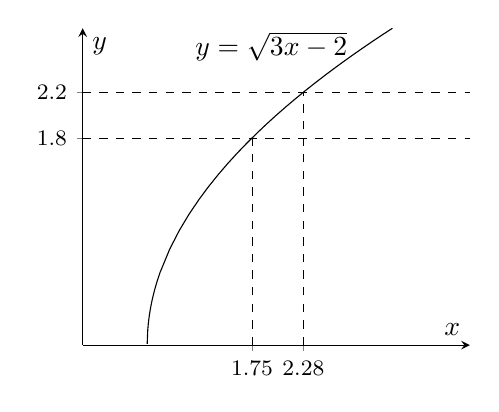
\begin{tikzpicture}
\begin{axis}[small,axis lines=middle,xlabel={$x$},ylabel={$y$},xtick={1.75,2.28},ytick={1.8,2.2}]
\addplot[domain=0.6667:0.8] {sqrt(3*x-2)};
\addplot[domain=0.8:3.2] {sqrt(3*x-2)}node[pos=0.9,left,xshift={-1mm}]{$y=\sqrt{3x-2}$};
\addplot[dashed] plot coordinates {(1.75,0) (1.75,1.8)};
\addplot[dashed]plot coordinates {(2.28,0) (2.28,2.2)};
\addplot[dashed] plot coordinates {(0,1.8) (4,1.8)};
\addplot[dashed]plot coordinates {(0,2.2) (4,2.2)};
\end{axis}
\end{tikzpicture}
\caption{$y$ کو $1.8$ اور $2.2$ کے اندر رکھنے کی خاطر $x$ کو $1.75$ اور $2.28$ کے اندر رکھنا ہو گا۔}
\label{شکل_مثال_حد_قابو_ب}
\end{minipage}
\end{figure}
\انتہا{مثال}
%==========================

\جزوحصہء{فنیات}
\ترچھا{مطلوبہ قیمتیں:}\quad
کمپیوٹر پر ترسیم کھینچ کر مطلوبہ قیمتوں پر تجربے کیے جا سکتے ہیں۔درکار تفاعل کی ترسیم پر بالائی اور نچلی مطلوبہ سطحوں کو افقی لکیروں سے ظاہر کریں۔ترسیم کو اتنا بڑا کریں کہ مطلوبہ وقفہ صاف نظر آئے۔یوں مطلوبہ وقفہ میں تفاعل کا رویہ دیکھا جا سکتا ہے۔

مثال کے طور پر \عددی{f(x)=\sqrt{3x-2}} کے ترسیم پر \عددی{y} محور کے مطلوبہ وقفہ \عددی{(1.8,2.2)} پر غور کریں۔یوں \عددی{y_1=f(x)}، \عددی{y_2=1.8} اور \عددی{y_3=2.2} ترسیم کریں (شکل \حوالہ{شکل_مثال_حد_قابو_ب})۔اسی طرح مطلوبہ وقفہ \عددی{(1.98,2.02)} اور \عددی{(1.9998,2.0002)} پر بھی تفاعل کا رویہ دیکھیں۔

\ابتدا{مثال}
\عددی{\SI{6}{\centi\meter}} اندرونی قطر کے ایک لڑر پیمائشی پیالے پر \عددی{\SI{1}{\milli\meter}} وقفہ پر افقی لکیریں کیوں کھینچی گئی ہوتی ہیں۔\\
پیالے میں مائع کا حجم \عددی{H=\pi r^2 h=36\pi h} ہو گا جہاں پیالے کا اندرونی رداس \عددی{r} اور مائع کی گہرائی \عددی{h} ہے۔ ایک لٹر \عددی{(\SI{1000}{\centi\meter\cubed})} پانی ناپنے کی خاطر \عددی{h} کتنا ہو گا؟ ناپ میں خلل \عددی{\SI{1}{\percent}} سے کم ہونا چاہیے۔\\
حل:\quad
ہم \عددی{h} کا ایسا وقفہ تلاش کرنا چاہتے ہیں کہ درج ذیل مطمئن ہوتا ہو۔
\begin{align*}
\abs{H-1000}=\abs{36\pi h-1000}\le 10
\end{align*}
یوں ہمیں درج ذیل عدم مساوات حل کرنی ہو گی۔
\begin{align*}
\abs{36\pi h-1000}&\le 10\\
-10\le 36\pi h-1000&\le 10\\
990\le 36\pi h&\le 1010\\
\tfrac{990}{36\pi}\le h &\le \tfrac{1010}{36\pi}\\
8.8\le h &\le 8.9
\end{align*}
یوں \عددی{\SI{1}{\percent}} درستگی کی خاطر درکار وقفہ گہرائی \عددی{8.9-8.8=\SI{0.1}{\centi\meter}} یعنی \عددی{\SI{1}{\milli\meter}} ہے۔پیالے پر ایک ملی میٹر فاصلے پر افقی لکیریں ہمیں ایک فی صد درستگی تک مائع ناپنے میں مدد دیتی ہیں جو کھانا تیار کرنے کے لئے کافی درستگی ہے۔
\انتہا{مثال}
%================

\جزوحصہء{حد کی با ضابطہ تعریف}
مطلوبہ قیمت مسئلے میں ہم جاننا چاہتے ہیں کہ متغیر \عددی{x} کو کسی مخصوص قیمت \عددی{x_0} کے کتنے قریب رکھتے ہوئے تفاعل \عددی{f(x)} کی قیمت کو مطلوبہ قیمت \عددی{y_0} کے قریب مخصوص وقفہ میں رکھنا ممکن ہو گا۔یہ دکھانے کی خاطر کہ \عددی{x\to x_0} کرنے سے \عددی{f(x)} کا حد \عددی{L} حاصل ہوتا ہے، ہمیں دکھانا ہو گا کہ ہم 
\عددی{x} کو \عددی{x_0} کے بہت قریب کرتے ہوئے  \عددی{f(x)} اور \عددی{L} میں فرق کو \ترچھا{کسی بھی معینہ خلل} سے کم کر سکتے ہیں۔

فرض کریں ہم  \عددی{f(x)} کی قیمت کو دیکھتے ہوئے \عددی{x} کو \عددی{x_0} کے قریب لاتے ہیں (تاہم  ہم \عددی{x} کی قیمت کو کبھی بھی \عددی{x_0} کے برابر نہیں کرتے ہیں)۔ہم چاہیں گے کہ ہم کہہ سکیں کہ \عددی{x_0} سے \عددی{x} کا فاصلہ \عددی{\delta} سے کم رکھنے سے \عددی{f(x)} اور \عددی{L} کی قیمت میں فرق \عددی{L} کی اکائی کے دسویں حصے  سے کم ہو گی (شکل \حوالہ{شکل_حد_تعریف_ایک_قدم})۔البتہ اتنا جاننا کافی نہیں ہے چونکہ \عددی{x} کو \عددی{x_0} کے مزید قریب کرنے سے کیا معلوم کہ وقفہ \عددی{L-\tfrac{1}{10}} تا \عددی{L+\tfrac{1}{10}} کے بیچ \عددی{f(x)} کی قیمت  \عددی{L} کے مزید قریب ہونے کی بجائے تھر تھراتی ہو۔
\begin{figure}
\centering
\begin{tikzpicture}
\draw[-latex](-0.25,0)--(4,0)node[right]{$x$};
\draw[-latex](0,-0.2)--(0,3.2)node[above]{$y$};
\draw(2,0)node[ocirc]{}node[below]{$x_0$};
\draw(1,0)node[]{$($}node[below]{$x_0-\delta$};
\draw(3,0)node[]{$)$}node[below]{$x_0+\delta$};
\draw(2.4,0)node[circ]{}node[above]{$x$};
\draw(0,1.5)node[left]{$L$}--++(0.1,0);
\draw(0,0.5)node[rotate=90]{$($}node[left,xshift={-1mm}]{$L-\tfrac{1}{10}$};
\draw(0,2.5)node[rotate=90]{$)$}node[left,xshift={-1mm}]{$L+\tfrac{1}{10}$};
\draw(0,2.1)node[circ]{}node[right]{$f(x)$};
\draw [decorate,decoration={brace,amplitude=10pt},yshift=10pt](1,0) -- (3,0)node [black,midway,yshift=15pt] {\footnotesize
\RL{یہاں تمام $x\ne x_0$ کے لئے}};
\draw [decorate,decoration={brace,amplitude=10pt},xshift=20pt](0,2.5) -- (0,0.5)node [black,midway,right,xshift=9pt] {\footnotesize
\RL{$f(x)$ یہاں رہے گا}};
\end{tikzpicture}
\caption{حد کی تعریف میں ایک قدم}
\label{شکل_حد_تعریف_ایک_قدم}
\end{figure}

ہمیں سے کہا جا سکتا ہے کہ  خلل میں چھوٹ \عددی{\tfrac{L}{100}} یا \عددی{\tfrac{L}{1000}} یا \عددی{\tfrac{L}{100,000}}  ہے۔ہر مرتبہ ہم \عددی {x_0} کے ارد گرد ایسا نیا وقفہ \عددی{\delta} تلاش کرتے ہیں جس کے اندر \عددی{x} کو رکھتے ہوئے قابل برداشت چھوٹ کے اندر رہا جا سکتا ہے۔البتہ ہر مرتبہ اس امکان کو رد نہیں کیا جا سکتا ہے کہ \عددی{x_0} کے مزید قریب جانے سے  \عددی{f(x)} کی قیمت تھر تھراہٹ کا شکار ہوتے  ہوئے \عددی{L} تک نہ پہنچتی ہو۔

شکل \حوالہ{شکل_حد_شکی_اور_عالم} میں اس مسئلے کی وضاحت کی گئی ہے جسے آپ ایک شکی انسان اور ایک عالم کے مابین بحث تصور کر سکتے ہیں۔شکی انسان قابل قبول چھوٹ  \عددی{\epsilon}  چاہتا ہے جس کے مقابلے میں عالم درکار \عددی{\delta} پیش کرتا ہے۔
\begin{figure}
\centering
\begin{subfigure}{0.5\textwidth}
\centering
\begin{tikzpicture}
\pgfmathsetmacro{\dY}{0.75}
\draw[-latex](0,0)--(4,0)node[right]{$x$};
\draw[-latex](0,0)--(0,2)node[above]{$y$};
\draw[name path=kC](0,0.10) to [out=45,in=-170] (2,1) to [out=10,in=-135](4,2);
\draw[dashed,name path=kA] (0,1+\dY)node[left]{$L+\tfrac{1}{10}$}--++(4,0);
\draw[dashed,name path=kB] (0,1-\dY)node[left]{$L-\tfrac{1}{10}$}--++(4,0);
\path[dashed,name path=kL](0,1)--++(4,0);
\draw[dashed,name intersections={of={kC and kL}}](0,1)--(intersection-1)node[circ]{}--($(0,0)!(intersection-1)!(4,0)$)node[below]{$x_0$};
\end{tikzpicture}
\caption{پہلا مقابلہ: $\abs{f(x)-L}< \epsilon=\tfrac{1}{10}$ کریں}
\end{subfigure}%
\begin{subfigure}{0.5\textwidth}
\centering
\begin{tikzpicture}
\pgfmathsetmacro{\dY}{0.75}
\draw[-latex](0,0)--(4,0)node[right]{$x$};
\draw[-latex](0,0)--(0,2)node[above]{$y$};
\draw[name path=kC](0,0.10) to [out=45,in=-170] (2,1) to [out=10,in=-135](4,2);
\draw[dashed,name path=kA] (0,1+\dY)node[left]{$L+\tfrac{1}{10}$}--++(4,0);
\draw[dashed,name path=kB] (0,1-\dY)node[left]{$L-\tfrac{1}{10}$}--++(4,0);
\path[dashed,name path=kL](0,1)--++(4,0);
\draw[dashed,name intersections={of={kC and kL}}](0,1)--(intersection-1)node[circ]{}--($(0,0)!(intersection-1)!(4,0)$)node[below]{$x_0$};
\draw[dashed,name intersections={of={kC and kA}}](0,1+\dY)--(intersection-1)--($(0,0)!(intersection-1)!(4,0)$)node[below]{$x_0-\delta_1$};
\draw[dashed,name intersections={of={kC and kB}}](0,1-\dY)--(intersection-1)--($(0,0)!(intersection-1)!(4,0)$)node[below]{$x_0+\delta_1$};
\end{tikzpicture}
\caption{پہلے جواب: $\abs{x-x_0}<\delta_1$ رکھیں}
\end{subfigure}
\begin{subfigure}{0.5\textwidth}
\centering
\begin{tikzpicture}
\pgfmathsetmacro{\dY}{0.35}
\draw[-latex](0,0)--(4,0)node[right]{$x$};
\draw[-latex](0,0)--(0,2)node[above]{$y$};
\draw[name path=kC](0,0.10) to [out=45,in=-170] (2,1) to [out=10,in=-135](4,2);
\draw[dashed,name path=kA] (0,1+\dY)node[left]{$L+\tfrac{1}{100}$}--++(4,0);
\draw[dashed,name path=kB] (0,1-\dY)node[left]{$L-\tfrac{1}{100}$}--++(4,0);
\path[dashed,name path=kL](0,1)--++(4,0);
\draw[dashed,name intersections={of={kC and kL}}](0,1)--(intersection-1)node[circ]{}--($(0,0)!(intersection-1)!(4,0)$)node[below]{$x_0$};
\end{tikzpicture}
\caption{دوسرا مقابلہ: $\abs{f(x)-L}< \epsilon=\tfrac{1}{100}$ کریں}
\end{subfigure}%
\begin{subfigure}{0.5\textwidth}
\centering
\begin{tikzpicture}
\pgfmathsetmacro{\dY}{0.35}
\draw[-latex](0,0)--(4,0)node[right]{$x$};
\draw[-latex](0,0)--(0,2)node[above]{$y$};
\draw[name path=kC](0,0.10) to [out=45,in=-170] (2,1) to [out=10,in=-135](4,2);
\draw[dashed,name path=kA] (0,1+\dY)node[left]{$L+\tfrac{1}{100}$}--++(4,0);
\draw[dashed,name path=kB] (0,1-\dY)node[left]{$L-\tfrac{1}{100}$}--++(4,0);
\path[dashed,name path=kL](0,1)--++(4,0);
\draw[dashed,name intersections={of={kC and kL}}](0,1)--(intersection-1)node[circ]{}--($(0,0)!(intersection-1)!(4,0)$)node[below]{$x_0$};
\draw[dashed,name intersections={of={kC and kA}}](0,1+\dY)--(intersection-1)--($(0,0)!(intersection-1)!(4,0)$)node[below]{$x_0-\delta_2$};
\draw[dashed,name intersections={of={kC and kB}}](0,1-\dY)--(intersection-1)--($(0,0)!(intersection-1)!(4,0)$)node[below]{$x_0+\delta_2$};
\end{tikzpicture}
\caption{دوسرا جواب: $\abs{x-x_0}<\delta_2$ رکھیں}
\end{subfigure}
\begin{subfigure}{0.5\textwidth}
\centering
\begin{tikzpicture}
\pgfmathsetmacro{\dY}{0.175}
\draw[-latex](0,0)--(4,0)node[right]{$x$};
\draw[-latex](0,0)--(0,2)node[above]{$y$};
\draw[name path=kC](0,0.10) to [out=45,in=-170] (2,1) to [out=10,in=-135](4,2);
\draw[dashed,name path=kA] (0,1+\dY)node[above left,solid]{$L+\tfrac{1}{1000}$}--++(4,0);
\draw[dashed,name path=kB] (0,1-\dY)node[below left,solid]{$L-\tfrac{1}{1000}$}--++(4,0);
\path[dashed,name path=kL](0,1)node[left]{$L$}--++(4,0);
\draw[dashed,name intersections={of={kC and kL}}](0,1)--(intersection-1)node[circ]{}--($(0,0)!(intersection-1)!(4,0)$)node[below]{$x_0$};
\end{tikzpicture}
\caption{تیسرا مقابلہ: $\abs{f(x)-L}< \epsilon=\tfrac{1}{1000}$ کریں}
\end{subfigure}%
\begin{subfigure}{0.5\textwidth}
\centering
\begin{tikzpicture}
\pgfmathsetmacro{\dY}{0.175}
\draw[-latex](0,0)--(4,0)node[right]{$x$};
\draw[-latex](0,0)--(0,2)node[above]{$y$};
\draw[name path=kC](0,0.10) to [out=45,in=-170] (2,1) to [out=10,in=-135](4,2);
\draw[dashed,name path=kA] (0,1+\dY)node[above left,solid]{$L+\tfrac{1}{1000}$}--++(4,0);
\draw[dashed,name path=kB] (0,1-\dY)node[below left,solid]{$L-\tfrac{1}{1000}$}--++(4,0);
\path[dashed,name path=kL](0,1)node[left]{$L$}--++(4,0);
\draw[dashed,name intersections={of={kC and kL}}](0,1)--(intersection-1)node[circ]{}--($(0,0)!(intersection-1)!(4,0)$)node[below]{$x_0$};
\draw[dashed,name intersections={of={kC and kA}}](0,1+\dY)--(intersection-1)--($(0,0)!(intersection-1)!(4,0)$)node[below,xshift={3mm}]{$x_0+\delta_3$};
\draw[dashed,name intersections={of={kC and kB}}](0,1-\dY)--(intersection-1)--($(0,0)!(intersection-1)!(4,0)$)node[below,xshift={-3mm}]{$x_0-\delta_3$};
\end{tikzpicture}
\caption{تیسرا جواب: $\abs{x-x_0}<\delta_3$ رکھیں}
\end{subfigure}%
\caption{شکی شخص اور عالم کا مقابلہ}
\label{شکل_حد_شکی_اور_عالم}
\end{figure}

اس نا ختم ہونے والی بحث کو ہم یوں ختم کر سکتے ہیں کہ ہم ثابت کریں کہ ہر \عددی{\sigma} کے لئے ایسا \عددی{\delta} تلاش کرنا ممکن ہے جو \عددی{f(x)} کو \عددی{L} کے  قریب قابل قبول فاصلہ \عددی{\epsilon} کے اندر رکھتا ہو (شکل \حوالہ{شکل_حد_تعریف})۔
\begin{figure}
\centering
\begin{tikzpicture}
\draw[-latex](-0.25,0)--(4,0)node[right]{$x$};
\draw[-latex](0,-0.2)--(0,3.2)node[above]{$y$};
\draw(2,0)node[ocirc]{}node[below]{$x_0$};
\draw(1,0)node[]{$($}node[below]{$x_0-\delta$};
\draw(3,0)node[]{$)$}node[below]{$x_0+\delta$};
\draw(2.4,0)node[circ]{}node[above]{$x$};
\draw(0,1.5)node[left]{$L$}--++(0.1,0);
\draw(0,0.5)node[rotate=90]{$($}node[left,xshift={-1mm}]{$L-\epsilon$};
\draw(0,2.5)node[rotate=90]{$)$}node[left,xshift={-1mm}]{$L+\epsilon$};
\draw(0,2.1)node[circ]{}node[right]{$f(x)$};
\draw [decorate,decoration={brace,amplitude=10pt},yshift=10pt](1,0) -- (3,0)node [black,midway,yshift=15pt] {\footnotesize
\RL{یہاں تمام $x\ne x_0$ کے لئے}};
\draw [decorate,decoration={brace,amplitude=10pt},xshift=20pt](0,2.5) -- (0,0.5)node [black,midway,right,xshift=9pt] {\footnotesize
\RL{$f(x)$ یہاں رہے گا}};
\end{tikzpicture}
\caption{حد کی تعریف میں $\delta$ اور $\epsilon$ کا تعلق۔}
\label{شکل_حد_تعریف}
\end{figure}

یوں آخر کار ہم ریاضی کی زبان میں یہ کہہ سکتے ہیں کہ \عددی{x} کو \عددی{x_0} کے جتنا زیادہ قریب کیا جائے، \عددی{f(x)} کی قیمت \عددی{L} کے اتنی قریب ہو گی۔

\ابتدا{تعریف}\موٹا{حد کی با ضابطہ تعریف}\\
فرض کریں کہ  \عددی{x_0} کے ارد گرد ایک کھلے وقفہ میں \عددی{f(x)} معین ہے جبکہ نقطہ \عددی{x_0} پر عین ممکن ہے کہ \عددی{f(x)} معین نہ ہو۔ اگر ہر عدد \عددی{\epsilon>0} کے لئے ایسا مطابقتی عدد \عددی{\delta>0} پایا جاتا ہو کہ تمام \عددی{x} کے لئے درج ذیل مطمئن ہوں  
\begin{align*}
0<\abs{x-x_0}<\delta,\quad \abs{f(x)-L}<\epsilon
\end{align*}
تب ہم کہتے ہیں کہ جیسے جیسے \عددی{x} کی قیمت \عددی{x_0} کے نزدیک تر ہوتی ہے  ویسے ویسے \عددی{f(x)} کی قیمت حد \عددی{L} تک پہنچتی ہے جس کو الجبرائی طور پر درج ذیل لکھا جاتا ہے۔
\begin{align*}
\lim_{x\to x_0} f(x)=L
\end{align*} 
\انتہا{تعریف}
%=========================

مطلوبہ قیمت کے تصور پر دوبارہ بات کرتے ہیں۔فرض کریں کہ آپ خراد کی مشین پر قطر \عددی{L} کا دھرا تیار کرنا چاہتے ہیں۔ اب کوئی بھی مشین مکمل درست نتائج نہیں دیتی ہے لہٰذا  آپ کو \عددی{f(x)} قطر یعنی \عددی{L-\epsilon} اور \عددی{L+\epsilon} کے بیچ قطر کا دھرا قبول کرنا ہو گا۔دھرا کا اتنا درست قطر حاصل کرنے کے لئے \عددی{x} کو قابو میں رکھنا ضروری ہو گا لہٰذا \عددی{x} کو \عددی{x-\delta} اور \عددی{x+\delta} کے بیچ رکھنا ہو گا۔ آپ دیکھ سکتے ہیں کہ جیسے جیسے قطر کی درستگی میں چھوٹ \عددی{\epsilon} کم کی جائے، آپ کو ویسے ویسے \عددی{\delta} کو درست کرنا ہو گا۔

\جزوحصہء{تعریف کو پرکھنے کی مثالیں}
حد کی با ضابطہ تعریف ہمیں حد تلاش کرنے میں مدد نہیں دیتی ہے البتہ اس سے حد کی درستگی کی تصدیق کی جا سکتی ہے۔درج ذیل مثالوں میں ہم حد کی تعریف کو استعمال کرتے ہوئے مخصوص تفاعل کی حد کی تصدیق کرتے ہیں۔حد کی تعریف کا اصل مقصد اس طرح کا حساب نہیں ہے بلکہ اس تعریف کو استعمال کرتے ہوئے عمومی مسئلے بیان کرنا مقصد ہے جو ہمیں تفاعل کی حد حاصل کرنے میں مدد دیتی ہیں۔
 
\ابتدا{مثال}\شناخت{مثال_حد_تلاش_مطلوبہ_الف}
دکھائیں کہ \عددی{\lim_{x\to1}(5x-3)=2} ہے۔\\
حل:\quad
حد کی تعریف میں \عددی{x_0=1}، \عددی{f(x)=5x-3} اور \عددی{L=2} لیں۔کسی بھی دیے گئے \عددی{\epsilon>0}  کے لئے ہمیں موزوں \عددی{\delta>0} تلاش کرنا ہو گا تا کہ اگر \عددی{x\ne 1} ہو اور \عددی{x_0=1} سے \عددی{x} کا فاصلہ \عددی{\delta} سے کم ہو یعنی اگر
\begin{align*}
0<\abs{x-a}<\delta
\end{align*}
ہو تب \عددی{L=2} سے \عددی{f(x)} کا فاصلہ \عددی{\epsilon} سے کم ہو گا یعنی:
\begin{align*}
\abs{f(x)-2}<\epsilon
\end{align*}
ہم \عددی{\epsilon} کی عدم مساوات سے واپس چلتے ہوئے \عددی{\delta} تلاش کرتے ہیں۔
\begin{align*}
\abs{(5x-3)-2}=\abs{5x-5}&<\epsilon\\
5\abs{x-1}&<\epsilon\\
\abs{x-1}&<\frac{\epsilon}{5}
\end{align*}
یوں ہم \عددی{\delta =\tfrac{\epsilon}{5}} لے سکتے ہیں (شکل \حوالہ{شکل_مثال_حد_تلاش_مطلوبہ_الف})۔اب اگر \عددی{0<\abs{x-1}<\delta=\tfrac{\epsilon}{5}} ہو تب درج ذیل ہو گا۔
\begin{align*}
\abs{(5x-3)-2}=\abs{5x-5}=5\abs{x-1}<5(\tfrac{\epsilon}{5})=\epsilon
\end{align*}
اس سے ثابت ہوا کہ \عددی{\lim_{x\to 1} (5x-3)=2} ہے۔

\عددی{\delta=\tfrac{\epsilon}{5}} وہ واحد قیمت نہیں ہے جس کے لئے \عددی{0<\abs{x-1}<\delta} سے مراد \عددی{\abs{5x-5}<\epsilon} لیا جا سکتا ہے۔\عددی{\delta} کی اس قیمت سے کوئی بھی چھوٹی مثبت قیمت کے لئے بھی \عددی{0<\abs{x-1}<\delta} سے مراد \عددی{\abs{5x-5}<\epsilon} لیا جا سکتا ہے۔حد کی تعریف بہترین \عددی{\delta} کی بات نہیں کرتی ہے بلکہ \عددی{\delta} کی کسی بھی قیمت جو ان شرائط کو مطمئن کرتا ہو کی بات کرتی ہے۔
\begin{figure}
\centering
\begin{tikzpicture}
\begin{axis}[clip=false,small,axis lines=middle,xlabel={$x$},ylabel={$y$},xlabel style={at={(current axis.right of origin)},anchor=west},xtick={0.8,1,1.2},xticklabels={$1-\tfrac{\epsilon}{5}$,$1$,$1+\tfrac{\epsilon}{5}$},ytick={-3,1,2,3},yticklabels={$-3$,$2-\epsilon$,$2$,$2+\epsilon$}]
\addplot[domain=-0.25:1.5]{5*x-3}node[left]{$y=5x-3$};
\draw[dashed](axis cs:0,2)--(axis cs:1,2)--(axis cs:1,0);
\draw[dashed](axis cs:0,1)--(axis cs:0.8,1)--(axis cs:0.8,0);
\draw[dashed](axis cs:0,3)--(axis cs:1.2,3)--(axis cs:1.2,0);
\end{axis}
\end{tikzpicture}
\caption{
تفاعل \عددی{f(x)=5x-3} کے لئے \عددی{0<\abs{x-1}<\tfrac{\epsilon}{5}} کی صورت میں \عددی{\abs{f(x)-2}<\epsilon} ہو گا (مثال \حوالہ{مثال_حد_تلاش_مطلوبہ_الف})۔
}
\label{شکل_مثال_حد_تلاش_مطلوبہ_الف}
\end{figure}
\انتہا{مثال}
%======================
\ابتدا{مثال}\شناخت{مثال_حد_تلاش_مطلوبہ_ب}\ترچھا{دو اہم حد}\\
تصدیق کریں: (ا)\quad 
$\lim_{x\to x_0} x=x_0$ 
\quad
(ب)\quad
$\lim_{x\to x_0}k=k$
جہاں \عددی{k} مستقل ہے۔ \\
حل:\quad
(ا)\quad
فرض کریں کہ \عددی{\epsilon>0} دیا گیا ہے۔ہمیں ایسا \عددی{\delta>0} تلاش کرنا ہے کہ تمام \عددی{x} کے لئے
\begin{align*}
\text{ہو۔}\quad\abs{x-x_0}<\epsilon \quad\text{\RL{سے مراد}}\quad 0<\abs{x-x_0}<\delta
\end{align*}
آپ دیکھ سکتے ہیں کہ \عددی{\delta} کی قیمت \عددی{\epsilon} کے برابر یا اس سے کم مثبت عدد ممکن ہے (شکل \حوالہ{شکل_مثال_حد_تلاش_مطلوبہ_ب}-ا)۔یوں ثابت ہو کہ \عددی{\lim_{x\to x_0}=x_0} ہے۔\\
(ب)\quad
فرض کریں کہ \عددی{\epsilon>0}  دیا گیا ہے۔ہمیں ایسا \عددی{\delta} تلاش کرنا ہے کہ ہر \عددی{x} کے لئے
\begin{align*}
\text{ہو۔}\quad\abs{k-k}<\epsilon \quad\text{\RL{سے مراد}}\quad 0<\abs{x-x_0}<\delta
\end{align*}
چونکہ \عددی{k-k=0} ہے لہٰذا کسی بھی مثبت عدد کو  \عددی{\delta} لیا جا سکتا ہے (شکل \حوالہ{شکل_مثال_حد_تلاش_مطلوبہ_ب}-ب)۔یوں ثابت ہوا کہ \عددی{\lim_{x\to x_0} k=k} ہے۔
\begin{figure}
\centering
\begin{subfigure}{0.45\textwidth}
\centering
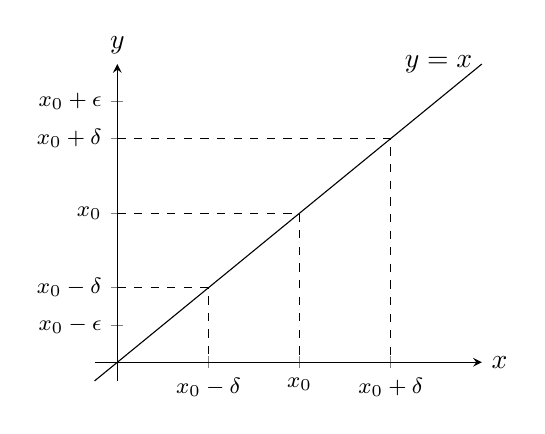
\begin{tikzpicture}
\begin{axis}[clip=false,small,axis lines=middle,xlabel={$x$},ylabel={$y$},xlabel style={at={(current axis.right of origin)},anchor=west},ylabel style={at={(current axis.above origin)},anchor=south},xtick={1,2,3},xticklabels={$x_0-\delta$,$x_0$,$x_0+\delta$},ytick={0.5,1,2,3,3.5},yticklabels={$x_0-\epsilon$,$x_0-\delta$,$x_0$,$x_0+\delta$,$x_0+\epsilon$}]
\addplot[domain=-0.25:4]{x}node[left]{$y=x$};
\draw[dashed](axis cs:0,2)--(axis cs:2,2)--(axis cs:2,0);
\draw[dashed](axis cs:0,1)--(axis cs:1,1)--(axis cs:1,0);
\draw[dashed](axis cs:0,3)--(axis cs:3,3)--(axis cs:3,0);
\end{axis}
\end{tikzpicture}
\caption{
\عددی{0<\abs{x-x_0}<\delta} کی صورت میں \عددی{f(x)=x} کے لئے جب بھی \عددی{\delta\le \epsilon} ہو تب  \عددی{\abs{f(x)-x_0}<\epsilon} ہو گا۔
}
\end{subfigure}\hfill
\begin{subfigure}{0.45\textwidth}
\centering
\begin{tikzpicture}
\begin{axis}[clip=false,small,axis lines=middle,xlabel={$x$},ylabel={$y$},xlabel style={at={(current axis.right of origin)},anchor=west},ylabel style={at={(current axis.above origin)},anchor=south},xtick={1,2,3},xticklabels={$x_0-\delta$,$x_0$,$x_0+\delta$},ytick={1,2,3},yticklabels={$k-\epsilon$,$k$,$k+\epsilon$},xmin=-0.25,ymin=0,ymax=5]
\addplot[domain=0:4]{2}node[pos=0.9,above]{$y=k$};
\draw[dashed](axis cs:1,2)--(axis cs:1,0);
\draw[dashed](axis cs:2,2)--(axis cs:2,0);
\draw[dashed](axis cs:3,2)--(axis cs:3,0);
\end{axis}
\end{tikzpicture}
\caption{
تفاعل \عددی{f(x)=k} کے لئے کسی بھی مثبت \عددی{\delta} کی صورت میں \عددی{\abs{f(x)-k}<\epsilon} ہو گا۔
}
\end{subfigure}%
\caption{اشکال برائے مثال \حوالہ{مثال_حد_تلاش_مطلوبہ_ب}}
\label{شکل_مثال_حد_تلاش_مطلوبہ_ب}
\end{figure}
\انتہا{مثال}
%==========================
\جزوحصہء{دیے گئے \عددی{\epsilon} کے لئے \عددی{\delta} کا الجبرائی حصول}
مثال \حوالہ{مثال_حد_تلاش_مطلوبہ_الف} اور مثال \حوالہ{مثال_حد_تلاش_مطلوبہ_ب} میں \عددی{x_0} کے ارد گرد وہ وقفہ جس پر \عددی{\abs{f(x)-L}} کی قیمت \عددی{\epsilon} سے کم تھی \عددی{x_0} کے لحاظ سے تشاکلی تھا۔یوں ہم \عددی{\delta} کو وقفہ کا نصف لے سکتے تھے۔جب ایسا تشاکل نہ پایا جاتا ہو، جو عموماً اوقات نہیں پایا جاتا ہے، ہم \عددی{x_0} سے وقفے کے قریبی سر تک فاصلے کو \عددی{\delta} لے سکتے ہیں۔ 

\ابتدا{مثال}\شناخت{مثال_حد_جذر_الف}
حد \عددی{\lim_{x\to 5}\sqrt{x-1}=2} کے لئے \عددی{\epsilon=1} کے لحاظ سے \عددی{\delta>0}  تلاش کریں۔یعنی ایسا \عددی{\delta>0} تلاش کریں کہ \عددی{0<\abs{x-5}<\delta} میں تمام \عددی{x} کے لئے درج ذیل مطمئن ہوتا ہو۔(علامت \عددی{\implies} کو پڑھیں "سے مراد"۔)
\begin{align*}
0<\abs{x-5}<\delta\quad \stackrel{\text{\RL{سے مراد}}}{\implies} \quad \abs{\sqrt{x-1}-2}<1
\end{align*}
حل:\quad
اس کو دو قدموں میں حل کرتے ہیں۔پہلی قدم میں عدم مساوات \عددی{\abs{\sqrt{x-1}-2}<1} کو حل کرتے ہوئے \عددی{x_0=5} کے ارد گرد ایسا وقفہ \عددی{(a,b)} تلاش کرتے ہیں جس پر تمام \عددی{x\ne x_0} کے لئے عدم مساوات مطمئن ہوتی ہو۔اس کے بعد ایسا عدد \عددی{\delta>0} حاصل کیا جائے گا کہ وقفہ \عددی{5-\delta<x<5+\delta} کا وسط نقطہ \عددی{x_0} ہو اور یہ وقفہ \عددی{(a,b)} کے اندر پایا جاتا ہو۔\\
\موٹا{پہلا قدم:}\quad
عدم مساوات \عددی{\abs{\sqrt{x-1}-2}<1} کو حل کرتے ہوئے \عددی{x_0=5} کے ارد گرد ایسا وقفہ تلاش کرتے ہیں کہ اس وقفے پر  تمام \عددی{x\ne x_0} کے لئے عدم مساوات مطمئن ہوتی ہو۔
\begin{align*}
\abs{\sqrt{x-1}-2}&<1\\
-1<\sqrt{x-1}-2&<1\\
1<\sqrt{x-1}&<3\\
1<x-1&<9\\
2<x&<10
\end{align*}
عدم مساوات کھلے وقفہ \عددی{(2,10)} پر تمام نقطوں کے لئے مطمئن ہوتی ہے لہٰذا یہ اس وقفے پر تمام \عددی{x\ne 5} کے لئے بھی مطمئن ہو گی۔\\
\موٹا{دوسرا قدم:}\quad
ایسا \عددی{\delta>0} تلاش کریں جو وسط کردہ وقفہ \عددی{5-\delta<x<5+\delta} کو وقفہ \عددی{(2,10)} میں رکھتا ہو۔\عددی{5} سے وقفہ \عددی{(2,10)} کے قریبی سر کا فاصلہ  \عددی{3} ہے۔اس طرح \عددی{\delta=3} یا اس سے کم کوئی بھی مثبت عدد لینے سے  \عددی{0<\abs{x-5}<\delta} کو مطمئن کرنے والے تمام \عددی{x} وقفہ \عددی{(2,10)} میں پائے جائیں گے جس سے  \عددی{\abs{\sqrt{x-1}-2}<1} خود بخود مطمئن ہو گا۔
\begin{align*}
0<\abs{x-5}<3\quad \implies\quad \abs{\sqrt{x-1}-2}<1
\end{align*}
%
\begin{figure}
\centering
\begin{subfigure}{0.45\textwidth}
\centering
\begin{tikzpicture}[x=0.5cm]
\draw[-latex](0,0)--(12,0)node[right]{$x$};
\foreach \x in {2,3,4,5,6,7,8,9,10}{\draw(\x,0)--++(0,0.1);}
\foreach \x in {2,5,8,10}{\draw(\x,0)node[below]{$\x$};}
\draw(5,0)node[ocirc]{};
\draw[-stealth](5-0.05,0.25)--(2,0.25)node[pos=0.5,above]{$3$};
\draw[-stealth](5+0.05,0.25)--(8,0.25)node[pos=0.5,above]{$3$};
\end{tikzpicture}
\caption{
\عددی{x_0=5} کے ارد گرد رداس \عددی{3} کا کھلا وقفہ \عددی{(2,10)} کے اندر پایا جائے گا۔
}
\end{subfigure}\hfill
\begin{subfigure}{0.45\textwidth}
\centering
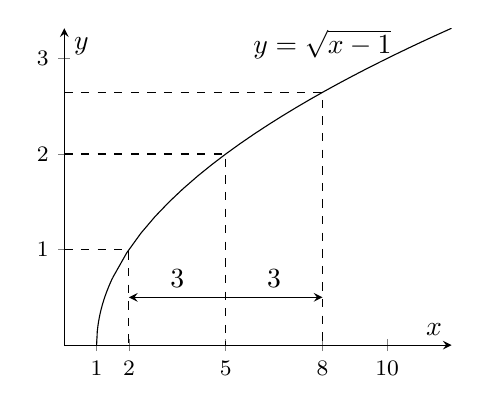
\begin{tikzpicture}
\begin{axis}[small,axis lines=middle,xlabel={$x$},ylabel={$y$},xtick={1,2,5,8,10},ytick={1,2,3}]
\addplot[domain=1:1.5]{sqrt(x-1)};
\addplot[domain=1.5:12]{sqrt(x-1)}node[left,xshift={-2mm},pos=0.9]{$y=\sqrt{x-1}$};
\addplot[dashed] plot coordinates {(0,2) (5,2) (5,0)};
\addplot[dashed] plot coordinates {(0,1) (2,1) (2,0)};
\addplot[dashed] plot coordinates {(0,2.646) (8,2.646) (8,0)};
\addplot[stealth-] plot coordinates {(2,0.5) (5,0.5)}node[pos=0.5,above]{$3$};
\addplot[stealth-] plot coordinates {(8,0.5) (5,0.5)}node[pos=0.5,above]{$3$};
\end{axis}
\end{tikzpicture}
\caption{تفاعل اور وقفہ}
\end{subfigure}%
\caption{اشکال برائے مثال \حوالہ{مثال_حد_جذر_الف}}
\label{شکل_مثال_حد_جذر_الف}
\end{figure}
\انتہا{مثال}
%======================
\جزوحصہء{دیے گئے \عددی{f}، \عددی{L}،\عددی{x_0} اور \عددی{\epsilon>0} کے لئے \عددی{\delta} کا الجبرائی حصول}
ایسا \عددی{\delta>0} کہ \عددی{0<\abs{x-x_0}<\delta} میں تمام \عددی{x} کے لئے درج ذیل ہو
\begin{align*}
0<\abs{x-x_0}<\delta\quad \implies \quad \abs{f(x)-L}<\epsilon
\end{align*}
 کو دو قدموں میں حاصل کیا جا سکتا ہے۔

\موٹا{پہلا قدم:}\quad
عدم مساوات \عددی{\abs{f(x)-L}<\epsilon} کو حل کرتے ہوئے \عددی{x_0} کے ارد گرد  ایسا کھلا وقفہ \عددی{(a,b)} حاصل کریں جس میں تمام \عددی{x\ne x_0} کے لئے  یہ  عدم مساوات مطمئن ہوتی ہو۔

\موٹا{دوسرا قدم:}\quad
ایسا \عددی{\delta>0} تلاش کریں جو کھلا وقفہ \عددی{(x_0-\delta,x_0+\delta)}، جس کا وسط \عددی{x_0} ہے، کو \عددی{(a,b)} کے اندر رکھے۔اس \عددی{\delta} وقفہ میں تمام \عددی{x\ne x_0} کے لئے عدم مساوات \عددی{\abs{f(x)-L}<\epsilon} مطمئن ہو گی۔

\ابتدا{مثال}
ثابت کریں کہ درج ذیل تفاعل کے لئے \عددی{\lim_{x\to 2}f(x)=4} ہے۔
\begin{align*}
f(x)=\begin{cases}
x^2,&x\ne 2\\
1,&x=2
\end{cases}
\end{align*}
حل:\quad
ہم نے ثابت کرنا ہے کہ دیے گئے \عددی{\epsilon>0} کے لئے ایسا \عددی{\delta>0} موجود ہے کہ \عددی{0<\abs{x-2}<\delta} میں تمام \عددی{x} کے لئے درج ذیل مطمئن ہوتا ہو۔
\begin{align*}
0<\abs{x-2}<\delta\quad \implies \quad \abs{f(x)-4}<\epsilon
\end{align*}
\موٹا{پہلا قدم:}\quad
عدم مساوات \عددی{\abs{f(x)-4}<\epsilon} کو حل کرتے ہوئے \عددی{x_0=2} کے ارد گرد ایسا کھلا وقفہ تلاش کرتے ہیں جس میں تمام \عددی{x\ne x_0} کے لئے عدم مساوات مطمئن ہوتی ہو۔اب \عددی{x\ne x_0=2} کے لئے \عددی{f(x)=x^2} ہے لہٰذا عدم مساوات کی صورت \عددی{\abs{x^2-4}<\epsilon} ہو گی۔ 
\begin{align*}
\abs{x^2-4}&<\epsilon\\
-\epsilon<x^2-4&<\epsilon\\
4-\epsilon<x^2&<4+\epsilon\\
\sqrt{4-\epsilon}<\abs{x}&<\sqrt{4+\epsilon}&&\text{\RL{فرض کریں کہ $\epsilon<4$ ہے}}\\
\sqrt{4-\epsilon}<x&<\sqrt{4+\epsilon}
\end{align*}
کھلا وقفہ \عددی{(\sqrt{4-\epsilon},\sqrt{4+\epsilon})} میں تمام \عددی{x\ne 2} کے لئے عدم مساوات \عددی{\abs{f(x)-4}<\epsilon} مطمئن ہوتی ہے۔

\موٹا{دوسرا قدم:}\quad
ایسا \عددی{\delta>0} تلاش کرتے ہیں جو وسط کردہ وقفہ \عددی{(2-\delta,2+\delta)} کو \عددی{(\sqrt{4-\epsilon},\sqrt{4+\epsilon})} کے اندر رکھتا ہو۔نقطہ \عددی{x_0=2} سے کھلا وقفہ \عددی{(\sqrt{4-\epsilon},\sqrt{4+\epsilon})} کے قریبی سر کا فاصلہ \عددی{\delta} ہو گا۔یوں \عددی{2-\sqrt{4-\epsilon}} اور \عددی{\sqrt{4+\epsilon}-2}  میں سے کم قیمت \عددی{\delta} کے برابر ہو گی۔\عددی{\delta} کی اس قیمت یا اس سے  کم مثبت قیمت کے لئے درج ذیل خود بخود مطمئن ہو گا۔
\begin{align*}
0<\abs{x-2}<\delta\quad \implies \quad \abs{f(x)-4}<\epsilon
\end{align*} 
\انتہا{مثال}
%==========================
درج بالا مثال میں ہم نے \عددی{\epsilon<4} کیوں فرض کیا؟ اس لئے کہ تمام \عددی{x} کے لئے ایسا \عددی{\delta} کہ \عددی{0<\abs{x-2}<\delta} سے مراد \عددی{\abs{f(x)-4}<\epsilon<4} ہو میں ہم نے \عددی{\delta} کی وہ قیمت دریافت کی جو \عددی{\epsilon} کے کسی بھی  بڑی قیمت کے لئے بھی کارآمد ہے۔

\جزوحصہء{مسئلوں کا ثبوت بذریعہ تعریف}
ہم عام طور پر حد کی با ضابطہ تعریف استعمال کرتے ہوئے مخصوص حد تلاش نہیں کرتے ہیں۔ اس کے برعکس ہم تعریف سے عمومی مسئلوں (بالخصوص حصہ \حوالہ{حصہ_حد_قواعد} کے مسئلوں) کو ثابت کرتے ہیں جنہیں استعمال کرتے ہوئے حد حاصل کیے جاتے ہیں۔آئیں  قاعدہ مجموعہ ثابت کریں۔

\ابتدا{مثال}\ترچھا{قاعدہ مجموعہ}\\
اگر \عددی{\lim_{x\to c}f(x)=L} اور \عددی{\lim_{z\to c} g(x)+M} ہوں تب درج ذیل ثابت کریں۔
\begin{align*}
\lim_{x\to c} (f(x)+g(x))=L+M
\end{align*}
حل:\quad
فرض کریں \عددی{\epsilon>0} دیا گیا ہے۔ہم ایسا مثبت عدد \عددی{\delta} تلاش کرنا چاہتے ہیں کہ \عددی{0<\abs{x-c}<\delta} میں  تمام \عددی{x} کے لئے درج ذیل ہو۔
\begin{align*}
0<\abs{x-c}<\delta\quad \implies \quad \abs{f(x)+g(x)-(L+M)}<\epsilon
\end{align*}
ہم ذیل لکھ سکتے ہیں۔
\begin{align*}
\abs{f(x)+g(x)-(L+M)}&=\abs{(f(x)-L)+(g(x)-M)}\\
&\le \abs{f(x)-L}+\abs{g(x)-M}&&\text{\RL{تکونی عدم مساوات}}
\end{align*}
چونکہ \عددی{\lim_{x\to c}f(x)=L} موجود ہے لہٰذا ایسا عدد \عددی{\delta_1>0} پایا جاتا ہے کہ تمام \عددی{x} کے لئے درج ذیل ہو۔
\begin{align*}
0<\abs{x-c}<\sigma_1\quad \implies\quad  \abs{f(x)-L}<\tfrac{\epsilon}{2}
\end{align*}
اسی طرح  چونکہ \عددی{\lim_{x\to c}g(x)=M} موجود ہے لہٰذا ایسا عدد \عددی{\delta_2>0} پایا جاتا ہے کہ تمام \عددی{x} کے لئے درج ذیل ہو۔
\begin{align*}
0<\abs{x-c}<\sigma_2\quad \implies\quad  \abs{g(x)-M}<\tfrac{\epsilon}{2}
\end{align*}
فرض کریں کہ \عددی{\delta_1} اور \عددی{\delta_2} میں سے چھوٹی قیمت \عددی{\delta} کے برابر  ہے۔اب اگر \عددی{0<\abs{x-c}<\delta} ہو تب
\begin{align*}
\abs{f(x)-L}<\tfrac{\epsilon}{2} \quad \text{اور}\quad 0<\abs{x-c}<\delta_1
\end{align*}
ہوں گے، اور \عددی{\abs{x-c}<\delta_2} اور \عددی{\abs{g(x)-M}<\tfrac{\epsilon}{2}} ہوں گے۔اس طرح 
\begin{align*}
\abs{f(x)+g(x)-(L+M)}<\frac{\epsilon}{2}+\frac{\epsilon}{2}=\epsilon
\end{align*}
ہو گا۔اس سے  ثابت ہوا کہ \عددی{\lim_{x\to c}(f(x)+g(x))=L+M} ہے۔
\انتہا{مثال}
%=====================

\حصہء{سوالات \حوالہ{حصہ_حد_مطلوبہ_قیمتیں_اور_حد}}

\موٹا{نقطہ \عددی{x_0} پر وقفے کا وسط لانا}\\
سوال \حوالہ{سوال_حد_وقفہ_ترسیم_وسط_الف} تا سوال \حوالہ{سوال_حد_وقفہ_ترسیم_وسط_ب} میں \عددی{x} محور پر وقفہ \عددی{(a,b)} ترسیم کریں جس میں نقطہ \عددی{x_0} پایا جاتا ہے۔اس کے بعد ایسا \عددی{\delta>0} تلاش کریں کہ \عددی{\abs{x-x_0}<\delta} سے مراد \عددی{a<x<b} ہو۔

\ابتدا{سوال}\شناخت{سوال_حد_وقفہ_ترسیم_وسط_الف}
$a=1,b=7,x_0=5$\\
جواب:\quad
$\delta=2$\quad
شکل \حوالہ{شکل_سوال_حد_وقفہ_ترسیم_وسط_الف}
\begin{figure}
\centering
\begin{minipage}{0.3\textwidth}
\centering
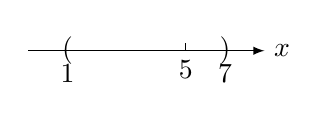
\begin{tikzpicture}
\draw[-latex](0,0)--(3,0)node[right]{$x$}; \draw(0.5,0)node[]{$($}node[below,yshift={-0.5mm}]{$1$} (2.5,0)node[]{$)$}node[below,yshift={-0.5mm}]{$7$} (2,0)node[below]{$5$}--++(0,0.1);
\end{tikzpicture}
\caption{}
\label{شکل_سوال_حد_وقفہ_ترسیم_وسط_الف}
\end{minipage}\hfill
\begin{minipage}{0.3\textwidth}
\centering
\begin{tikzpicture}
\draw[-latex](0,0)--(3,0)node[right]{$x$}; \draw(0.5,0)node[]{$($}node[below,yshift={-0.5mm}]{$-\tfrac{7}{2}$} (2.5,0)node[]{$)$}node[below,yshift={-0.5mm}]{$-\tfrac{1}{2}$} (1,0)node[below]{$-3$}--++(0,0.1);
\end{tikzpicture}
\caption{}
\label{شکل_سوال_حد_وقفہ_ترسیم_وسط_درکار_ب}
\end{minipage}\hfill
\begin{minipage}{0.3\textwidth}
\centering
\begin{tikzpicture}
\draw[-latex](0,0)--(3,0)node[right]{$x$}; \draw(0.5,0)node[]{$($}node[below,yshift={-0.5mm}]{$\tfrac{4}{9}$} (2.5,0)node[]{$)$}node[below,yshift={-0.5mm}]{$\tfrac{4}{7}$} (1.25,0)node[below]{$\tfrac{1}{2}$}--++(0,0.1);
\end{tikzpicture}
\caption{}
\label{شکل_سوال_حد_وقفہ_ترسیم_وسط_درکار_پ}
\end{minipage}%
\end{figure}
\انتہا{سوال}
%=======================
\ابتدا{سوال}
$a=1,b=7,x_0=2$
\انتہا{سوال}
%=======================
\ابتدا{سوال}
$a=-\tfrac{7}{2},b=-\tfrac{1}{2},x_0=-3$\\
جواب:\quad
$\delta=\tfrac{1}{2}$\quad
شکل \حوالہ{شکل_سوال_حد_وقفہ_ترسیم_وسط_درکار_ب}
\انتہا{سوال}
%=======================
\ابتدا{سوال}
$a=-\tfrac{7}{2},b=-\tfrac{1}{2},x_0=-\tfrac{3}{2}$
\انتہا{سوال}
%=======================
\ابتدا{سوال}
$a=\tfrac{4}{9},b=\tfrac{4}{7},x_0=\tfrac{1}{2}$\\
جواب:\quad
$\delta=\tfrac{1}{18}$\quad
شکل \حوالہ{شکل_سوال_حد_وقفہ_ترسیم_وسط_درکار_پ}
\انتہا{سوال}
%=======================
\ابتدا{سوال}\شناخت{سوال_حد_وقفہ_ترسیم_وسط_ب}
$a=2.7591,b=3.2391,x_0=3$
\انتہا{سوال}
%=======================

\موٹا{\عددی{\delta} کا حصول بذریعہ ترسیم}\\
سوال \حوالہ{سوال_حد_ترسیم_ڈیلٹا_الف} تا سوال \حوالہ{سوال_حد_ترسیم_ڈیلٹا_ب} میں ترسیم سے ایسا \عددی{\delta>0} تلاش کریں کہ تمام \عددی{x} کے لئے درج ذیل ہو۔
\begin{align*}
0<\abs{x-x_0}<\delta\quad \implies \quad 0<\abs{f(x)-L}<\epsilon
\end{align*}

\ابتدا{سوال}\شناخت{سوال_حد_ترسیم_ڈیلٹا_الف}
$f(x)=2x-4,x_0=5, L=6,\epsilon=0.2$\quad
شکل \حوالہ{شکل_سوال_حد_ترسیم_ڈیلٹا_الف}\\
جواب:\quad
$\delta=0.1$
%
\begin{figure}
\centering
\begin{minipage}{0.45\textwidth}
\centering
\begin{tikzpicture}[font=\small]
\draw[-latex](-0.25,0)--(4,0)node[right]{$x$};
\draw[-latex](0,-0.2)--(0,2)node[above]{$y$};
\draw[name path=kC](0.25,-0.5)--(4,2)node[pos=0.9,left,xshift={-2mm}]{$y=2x-4$};
\path[name path=kA](0,1)--++(4,0);
\draw[dashed,name intersections={of=kA and kC}](0,1)node[left]{$6$}--(intersection-1)--($(0,0)!(intersection-1)!(4,0)$)node[below]{$5$};
\path[name path=kA](0,0.5)--++(4,0);
\draw[dashed,name intersections={of=kA and kC}](0,0.5)node[left]{$5.8$}--(intersection-1)--($(0,0)!(intersection-1)!(4,0)$)node[below]{$4.9$};
\path[name path=kA](0,1.5)--++(4,0);
\draw[dashed,name intersections={of=kA and kC}](0,1.5)node[left]{$6$}--(intersection-1)--($(0,0)!(intersection-1)!(4,0)$)node[below]{$5.1$};
\end{tikzpicture}
\caption{ترسیم برائے سوال \حوالہ{سوال_حد_ترسیم_ڈیلٹا_الف}}
\label{شکل_سوال_حد_ترسیم_ڈیلٹا_الف}
\end{minipage}\hfill
\begin{minipage}{0.45\textwidth}
\centering
\begin{tikzpicture}[font=\small]
\draw[-latex](-4,0)--(0.2,0)node[right]{$x$};
\draw[-latex](0,-0.2)--(0,2)node[above]{$y$};
\draw[name path=kC,shorten >=-0.5cm](0.25,0.25)--(-4,2)node[pos=0.75,above right]{$y=-\tfrac{3}{2}x+3$};
\path[name path=kA](0,1)--++(-4,0);
\draw[dashed,name intersections={of=kA and kC}](0,1)node[right]{$7.5$}--(intersection-1)--($(0,0)!(intersection-1)!(-4,0)$)node[below]{$-3$};
\path[name path=kA](0,1.3)--++(-4,0);
\draw[dashed,name intersections={of=kA and kC}](0,1.3)node[right]{$7.65$}--(intersection-1)--($(0,0)!(intersection-1)!(-4,0)$)node[below]{$-3.1$};
\path[name path=kA](0,0.7)--++(-4,0);
\draw[dashed,name intersections={of=kA and kC}](0,0.7)node[right]{$7.35$}--(intersection-1)--($(0,0)!(intersection-1)!(-4,0)$)node[below]{$-2.9$};
\end{tikzpicture}
\caption{ترسیم برائے سوال \حوالہ{سوال_حد_ترسیم_ڈیلٹا_پ}}
\label{شکل_سوال_حد_ترسیم_ڈیلٹا_پ}
\end{minipage}%
\end{figure}
\انتہا{سوال}
%========================
\ابتدا{سوال}\شناخت{سوال_حد_ترسیم_ڈیلٹا_پ}
$f(x)=-\tfrac{3}{2}x+3,x_0=-3,L=7.5,\epsilon=0.15$\quad
شکل \حوالہ{شکل_سوال_حد_ترسیم_ڈیلٹا_پ}
\انتہا{سوال}
%=======================
\ابتدا{سوال}\شناخت{سوال_حد_ترسیم_ڈیلٹا_ت}
$f(x)=\sqrt{x},x_0=1,L=1,\epsilon=\tfrac{1}{4}$\quad
شکل \حوالہ{شکل_سوال_حد_ترسیم_ڈیلٹا_ت}\\
جواب:\quad
$\delta=\tfrac{7}{16}$
%
\begin{figure}
\centering
\begin{minipage}{0.45\textwidth}
\centering
\begin{tikzpicture}
\begin{axis}[small,axis lines=middle,xlabel={$x$},ylabel={$y$},xtick={0.5625,1,1.5625},xticklabels={$\tfrac{9}{16}$,$1$,$\tfrac{25}{16}$},ytick={0.75,1,1.25},yticklabels={$\tfrac{3}{4}$,$1$,$\tfrac{5}{4}$}]
\addplot[domain=0:0.5]{sqrt(x)};
\addplot[domain=0.5:3]{sqrt(x)}node[pos=0.6,below right]{$y=\sqrt{x}$};
\addplot[dashed] plot coordinates {(0,0.75)(0.5625,0.75)(0.5625,0)};
\addplot[dashed] plot coordinates {(0,1)(1,1)(1,0)};
\addplot[dashed] plot coordinates {(0,1.25)(1.5625,1.25)(1.5625,0)};
\end{axis}
\end{tikzpicture}
\caption{ترسیم برائے سوال \حوالہ{سوال_حد_ترسیم_ڈیلٹا_ت}}
\label{شکل_سوال_حد_ترسیم_ڈیلٹا_ت}
\end{minipage}\hfill
\begin{minipage}{0.45\textwidth}
\centering
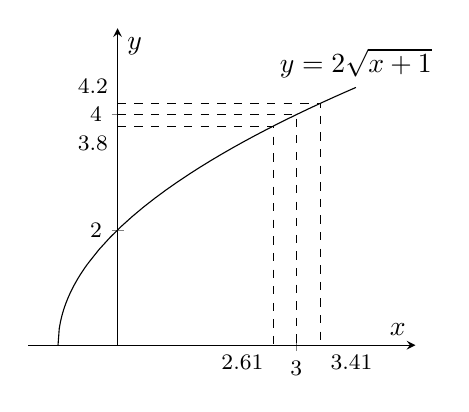
\begin{tikzpicture}
\begin{axis}[clip=false,small,axis lines=middle,xlabel={$x$},ylabel={$y$},xtick={3},ytick={2,4},ymax=5.5,ymin=0,xmin=-1.5,xmax=5]
\addplot[domain=-1:-0.5]{2*sqrt(x+1)};
\addplot[domain=-0.5:4]{2*sqrt(x+1)}node[pos=1,above]{$y=2\sqrt{x+1}$};
\addplot[dashed] plot coordinates {(0,4.2)(3.41,4.2)(3.41,0)};
\addplot[dashed] plot coordinates {(0,4)(3,4)(3,0)};
\addplot[dashed] plot coordinates {(0,3.8)(2.61,3.8)(2.61,0)};
\draw(axis cs:0,4.2)node[above left,font=\footnotesize]{$4.2$}  (axis cs:0,3.8)node[below left,font=\footnotesize]{$3.8$};
\draw(axis cs:2.61,0)node[below left,font=\footnotesize]{$2.61$}  (axis cs:3.41,0)node[below right,font=\footnotesize]{$3.41$};
\end{axis}
\end{tikzpicture}
\caption{ترسیم برائے سوال \حوالہ{سوال_حد_ترسیم_ڈیلٹا_ٹ}}
\label{شکل_سوال_حد_ترسیم_ڈیلٹا_ٹ}
\end{minipage}%
\end{figure}
\انتہا{سوال}
%=============================
\ابتدا{سوال}\شناخت{سوال_حد_ترسیم_ڈیلٹا_ٹ}
$f(x)=2\sqrt{x+1},x_0=3,L=4,\epsilon=0.2$\quad
شکل \حوالہ{شکل_سوال_حد_ترسیم_ڈیلٹا_ٹ}
\انتہا{سوال}
%=====================

\ابتدا{سوال}\شناخت{سوال_حد_ترسیم_ڈیلٹا_ث}
$f(x)=x^2,x_0=2,L=4,\epsilon=1$\quad
شکل \حوالہ{شکل_سوال_حد_ترسیم_ڈیلٹا_ث}\\
جواب:\quad
$\delta=\sqrt{5}-2$
%
\begin{figure}
\centering
\begin{minipage}{0.45\textwidth}
\centering
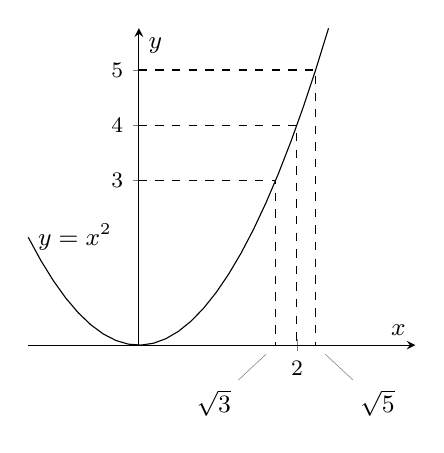
\begin{tikzpicture}[font=\small]
\begin{axis}[clip=false,small,axis lines=middle,xlabel={$x$},ylabel={$y$},xtick={2},ytick={3,4,5},xmax=3.5]
\addplot[domain=-1.4:2.4]{x^2}node[pos=0,right]{$y=x^2$};
\addplot[dashed] plot coordinates {(0,3)(1.732,3)(1.732,0)};
\addplot[dashed] plot coordinates {(0,4)(2,4)(2,0)};
\addplot[dashed] plot coordinates {(0,5)(2.236,5)(2.236,0)};
\draw(axis cs:1.732,0)node[pin=-135:{$\sqrt{3}$}]{};
\draw(axis cs:2.236,0)node[pin=-45:{$\sqrt{5}$}]{};
\end{axis}
\end{tikzpicture}
\caption{ترسیم برائے سوال \حوالہ{سوال_حد_ترسیم_ڈیلٹا_ث}}
\label{شکل_سوال_حد_ترسیم_ڈیلٹا_ث}
\end{minipage}\hfill
\begin{minipage}{0.45\textwidth}
\centering
\begin{tikzpicture}[font=\small]
\begin{axis}[clip=false,small,axis lines=middle,xlabel={$x$},ylabel={$y$},xtick={-1},ytick={3},yticklabel style={anchor=west,xshift={1mm}},ymax=4.5]
\addplot[domain=-2:0.25]{4-x^2}node[pos=0.75,above left]{$y=4-x^2$};
\addplot[dashed] plot coordinates {(0,3.25)(-0.866,3.25)(-0.866,0)};
\addplot[dashed] plot coordinates {(0,3)(-1,3)(-1,0)};
\addplot[dashed] plot coordinates {(0,2.75)(-1.118,2.75)(-1.118,0)};
\draw(axis cs:0,3.25)node[pin=10:{$3.25$}]{}  (axis cs:0,2.75)node[pin=-10:{$2.75$}]{};
\draw(axis cs:-1.118,0)node[pin=-135:{$-\tfrac{5}{2}$}]{}  (axis cs:-0.866,0)node[pin=-45:{$-\tfrac{3}{2}$}]{};
\end{axis}
\end{tikzpicture}
\caption{ترسیم برائے سوال \حوالہ{سوال_حد_ترسیم_ڈیلٹا_ج}}
\label{شکل_سوال_حد_ترسیم_ڈیلٹا_ج}
\end{minipage}%
\end{figure}
\انتہا{سوال}
%=============================
\ابتدا{سوال}\شناخت{سوال_حد_ترسیم_ڈیلٹا_ج}
$f(x)=4-x^2,x_0=-1,L=3,\epsilon=0.25$\quad
شکل \حوالہ{شکل_سوال_حد_ترسیم_ڈیلٹا_ج}
\انتہا{سوال}
%=====================
\ابتدا{سوال}\شناخت{سوال_حد_ترسیم_ڈیلٹا_چ}
$f(x)=\tfrac{2}{\sqrt{-x}},x_0=-1,L=2,\epsilon=0.5$\quad
شکل \حوالہ{شکل_سوال_حد_ترسیم_ڈیلٹا_چ}\\
جواب:\quad
$\delta=0.36$
%

\begin{figure}
\centering
\begin{minipage}{0.45\textwidth}
\centering
\begin{tikzpicture}[font=\small]
\begin{axis}[clip=false,small,axis lines=middle,xlabel={$x$},ylabel={$y$},xtick={-1.7778,-1,-0.64},xticklabels={$-\tfrac{16}{9}$,$-1$,$-\tfrac{16}{25}$},ytick={1.5,2,2.5},yticklabel style={anchor=west,xshift={1mm}}]
\addplot[domain=-2:-0.25]{2/sqrt(-x)}node[pos=0.75,above left]{$y=\tfrac{2}{\sqrt{-x}}$};
\addplot[dashed] plot coordinates {(0,1.5)(-1.7778,1.5)(-1.7778,0)};
\addplot[dashed] plot coordinates {(0,2)(-1,2)(-1,0)};
\addplot[dashed] plot coordinates {(0,2.5)(-0.64,2.5)(-0.64,0)};
%\draw(axis cs:1.732,0)node[pin=-135:{$\sqrt{3}$}]{};
%\draw(axis cs:2.236,0)node[pin=-45:{$\sqrt{5}$}]{};
\end{axis}
\end{tikzpicture}
\caption{ترسیم برائے سوال \حوالہ{سوال_حد_ترسیم_ڈیلٹا_چ}}
\label{شکل_سوال_حد_ترسیم_ڈیلٹا_چ}
\end{minipage}\hfill
\begin{minipage}{0.45\textwidth}
\centering
\begin{tikzpicture}[font=\small]
\begin{axis}[clip=false,small,axis lines=middle,xlabel={$x$},ylabel={$y$},xmin=0,ymin=0,xtick={\empty},ytick={\empty}]
\addplot[name path=kC,domain=0.25:0.75]{1/x}node[pos=0.25,above right]{$y=\tfrac{1}{x}$};
\path[name path=kA](axis cs:0,2)--(axis cs:1,2);
\draw[dashed,name intersections={of={kA and kC}}](axis cs:0,2)node[left]{$1.99$}--(intersection-1)--($(axis cs:0,0)!(intersection-1)!(axis cs:1,0)$)node[below]{$\tfrac{1}{1.99}$};
\path[name path=kA](axis cs:0,2.3)--(axis cs:1,2.3);
\draw[dashed,name intersections={of={kA and kC}}](axis cs:0,2.3)node[left]{$2$}--(intersection-1)--($(axis cs:0,0)!(intersection-1)!(axis cs:1,0)$)node[below]{$\tfrac{1}{2}$};
\path[name path=kA](axis cs:0,3)--(axis cs:1,3);
\draw[dashed,name intersections={of={kA and kC}}](axis cs:0,3)node[left]{$2.01$}--(intersection-1)--($(axis cs:0,0)!(intersection-1)!(axis cs:1,0)$)node[below]{$\tfrac{1}{2.01}$};
\end{axis}
\end{tikzpicture}
\caption{ترسیم برائے سوال \حوالہ{سوال_حد_ترسیم_ڈیلٹا_ب}}
\label{شکل_سوال_حد_ترسیم_ڈیلٹا_ب}
\end{minipage}%
\end{figure}
\انتہا{سوال}
%======================
\ابتدا{سوال}\شناخت{سوال_حد_ترسیم_ڈیلٹا_ب}
$f(x)=\tfrac{1}{x},x_0=\tfrac{1}{2},L=2,\epsilon=0.01$\quad
شکل \حوالہ{شکل_سوال_حد_ترسیم_ڈیلٹا_ب}

\انتہا{سوال}
%=====================
\موٹا{\عددی{\delta} کا الجبرائی حصول}\\
سوال \حوالہ{سوال_حد_تلاش_ڈیلٹا_الجبرائی_الف} تا سوال \حوالہ{سوال_حد_تلاش_ڈیلٹا_الجبرائی_ب} میں \عددی{f(x)} اور اعداد  \عددی{L}، \عددی{x_0} اور \عددی{\epsilon>0} دیے گئے ہیں۔ہر سوال میں \عددی{x_0} کے ارد گرد ایسا کھلا وقفہ تلاش کریں جس پر عدم مساوات \عددی{\abs{f(x)-L}<\epsilon} مطمئن ہوتی ہو۔اس کے بعد \عددی{\delta>0}  کی ایسی قیمت تلاش کریں کہ  عدم مساوات \عددی{0<\abs{x-x_0}<\delta} کو مطمئن کرنے والے ہر \عددی{x} کے لئے عدم مساوات \عددی{\abs{f(x)-L}<\epsilon} مطمئن ہوتی ہے۔ 

\ابتدا{سوال}\شناخت{سوال_حد_تلاش_ڈیلٹا_الجبرائی_الف}
$f(x)=x+1,L=5,x_0=4,\epsilon=0.01$\\
جواب:\quad
$\delta=0.01,\quad (3.99,4.01)$
\انتہا{سوال}
%========================
\ابتدا{سوال}
$f(x)=2x-2,L=-6,x_0=-2,\epsilon=0.02$
\انتہا{سوال}
%========================
\ابتدا{سوال}
$f(x)=\sqrt{x+1},L=1,x_0=0,\epsilon=0.1$\\
جواب:\quad
$\delta=0.19,\quad (-0.19,0.21)$
\انتہا{سوال}
%========================
\ابتدا{سوال}
$f(x)=\sqrt{x},L=\tfrac{1}{2},x_0=\tfrac{1}{4},\epsilon=0.1$
\انتہا{سوال}
%========================
\ابتدا{سوال}
$f(x)=\sqrt{19-x},L=3,x_0=10,\epsilon=1$\\
جواب:\quad
$\delta=5,\quad (3,15)$
\انتہا{سوال}
%========================
\ابتدا{سوال}
$f(x)=\sqrt{x-7},L=4,x_0=23,\epsilon=1$
\انتہا{سوال}
%========================
\ابتدا{سوال}
$f(x)=\tfrac{1}{x},L=\tfrac{1}{4},x_0=4,\epsilon=0.05$\\
جواب:\quad
$\delta=\tfrac{2}{3},\quad (\tfrac{10}{3},5)$
\انتہا{سوال}
%========================
\ابتدا{سوال}
$f(x)=x^2,L=3,x_0=\sqrt{3},\epsilon=0.1$
\انتہا{سوال}
%========================
\ابتدا{سوال}
$f(x)=x^2,L=4,x_0=-2,\epsilon=0.5$\\
جواب:\quad
$\delta=\sqrt{4.5}-2\approx 0.12,\quad (-\sqrt{4.5},-\sqrt{3.5})$
\انتہا{سوال}
%========================
\ابتدا{سوال}
$f(x)=\tfrac{1}{x},L=-1,x_0=-1,\epsilon=0.1$
\انتہا{سوال}
%========================
\ابتدا{سوال}
$f(x)=x^2-5,L=11,x_0=4,\epsilon=1$\\
جواب:\quad
$\delta=\sqrt{17}-4\approx 0.12,\quad (\sqrt{15},\sqrt{17})$
\انتہا{سوال}
%========================
\ابتدا{سوال}
$f(x)=\tfrac{120}{x},L=5,x_0=24,\epsilon=1$
\انتہا{سوال}
%========================
\ابتدا{سوال}
$f(x)=mx,m>0,L=2m,x_0=2,\epsilon=0.03$\\
جواب:\quad
$\delta=\tfrac{0.03}{m},\quad (2-\tfrac{0.03}{m},2+\tfrac{0.03}{m})$
\انتہا{سوال}
%========================
\ابتدا{سوال}
$f(x)=mx,m>0,L=3m,x_0=3,\epsilon=c>0$
\انتہا{سوال}
%========================
\ابتدا{سوال}
$f(x)=mx+b,m>0,L=\tfrac{m}{2}+b,x_0=\tfrac{1}{2},\epsilon=c>0$\\
جواب:\quad
$\delta=\tfrac{c}{m},\quad (\tfrac{1}{2}-\tfrac{c}{m},\tfrac{1}{2}+\tfrac{c}{m})$
\انتہا{سوال}
%========================
\ابتدا{سوال}\شناخت{سوال_حد_تلاش_ڈیلٹا_الجبرائی_ب}
$f(x)=mx+b,m>0,L=m+b,x_0=1,\epsilon=0.05$
\انتہا{سوال}
%========================
\موٹا{با ضابطہ حد پر مزید سوالات}\\
سوال \حوالہ{سوال_حد_مزید_الف} تا سوال \حوالہ{سوال_حد_مزید_ب} میں تفاعل \عددی{f(x)}، نقطہ \عددی{x_0} اور مثبت عدد \عددی{\epsilon} دیے گئے ہیں۔\عددی{\lim\limits_{x\to x_0}f(x)} تلاش کریں۔اس کے بعد ایسا عدد \عددی{\delta>0} تلاش کریں کہ تمام \عددی{x} کے لئے درج ذیل ہو۔
\begin{align*}
0<\abs{x-x_0}<\delta\quad \implies \quad \abs{f(x)-L}<\epsilon
\end{align*} 

\ابتدا{سوال}\شناخت{سوال_حد_مزید_الف}
$f(x)=3-2x,x_0=3,\epsilon=0.02$\\
جواب:\quad
$\delta=0.01,\quad L=-3$
\انتہا{سوال}
%=====================
\ابتدا{سوال}
$f(x)=-3x-2,x_0=-1,\epsilon=0.03$
\انتہا{سوال}
%=====================
\ابتدا{سوال}
$f(x)=\tfrac{x^2-4}{x-2},x_0=2,\epsilon=0.05$\\
جواب:\quad
$\delta=0.05,\quad L=4$
\انتہا{سوال}
%=====================
\ابتدا{سوال}
$f(x)=\tfrac{x^2+6x+5}{x+5},x_0=-5,\epsilon=0.05$
\انتہا{سوال}
%=====================
\ابتدا{سوال}
$f(x)=\sqrt{1-5x},x_0=-3,\epsilon=0.5$\\
جواب:\quad
$\delta=0.75,\quad L=4$
\انتہا{سوال}
%=====================
\ابتدا{سوال}\شناخت{سوال_حد_مزید_ب}
$f(x)=\tfrac{4}{x},x_0=2,\epsilon=0.4$
\انتہا{سوال}
%=====================

سوال \حوالہ{سوال_حد_فقرہ_الف} تا سوال \حوالہ{سوال_حد_فقرہ_ب} میں دیا گیا فقرہ حد ثابت کریں۔

\ابتدا{سوال}\شناخت{سوال_حد_فقرہ_الف}
$\lim\limits_{x\to 4} (9-x)=5$
\انتہا{سوال}
%=====================
\ابتدا{سوال}
$\lim\limits_{x\to 3} (3x-7)=2$
\انتہا{سوال}
%=====================
\ابتدا{سوال}
$\lim\limits_{x\to 9} \sqrt{x-5}=2$
\انتہا{سوال}
%=====================
\ابتدا{سوال}
$\lim\limits_{x\to 0} \sqrt{4-x}=2$
\انتہا{سوال}
%=====================
\ابتدا{سوال}
$f(x)=\begin{cases} x^2,&x\ne 1\\ 2,&x=1 \end{cases}$\,\,
کے لئے \,\,
$\lim\limits_{x\to 1} f(x)=1$
\انتہا{سوال}
%=====================
\ابتدا{سوال}
$f(x)=\begin{cases} x^2,&x\ne -2\\ 1,&x=-2 \end{cases}$\,\,
کے لئے \,\,
$\lim\limits_{x\to -2} f(x)=4$
\انتہا{سوال}
%=====================
\ابتدا{سوال}
$\lim\limits_{x\to 1} \tfrac{1}{x}=1$
\انتہا{سوال}
%=====================
\ابتدا{سوال}
$\lim\limits_{x\to \sqrt{3}} \tfrac{1}{x^2}=\tfrac{1}{3}$
\انتہا{سوال}
%=====================
\ابتدا{سوال}
$\lim\limits_{x\to -3} \tfrac{x^2-9}{x+3}=-6$
\انتہا{سوال}
%=====================
\ابتدا{سوال}
$\lim\limits_{x\to 1} \tfrac{x^2-1}{x-1}=2$
\انتہا{سوال}
%=====================
\ابتدا{سوال}
$f(x)=\begin{cases} 4-2x,&x<1\\ 6x-4,&x\ge 1 \end{cases}$\,\,
کے لئے \,\,
$\lim\limits_{x\to 1} f(x)=2$
\انتہا{سوال}
%=====================
\ابتدا{سوال}
$f(x)=\begin{cases} 2x,&x<0\\  \tfrac{x}{2},&x\ge 0 \end{cases}$\,\,
کے لئے \,\,
$\lim\limits_{x\to 0} f(x)=0$
\انتہا{سوال}
%=====================
\ابتدا{سوال}\شناخت{سوال_حد_فقرہ_پ}
$\lim\limits_{x\to 0} x\sin \tfrac{1}{x}=0$\quad
شکل \حوالہ{شکل_سوال_حد_فقرہ_پ}
\begin{figure}
\centering
\begin{minipage}{0.45\textwidth}
\centering
\begin{tikzpicture}
\begin{axis}[clip=false,scaled x ticks=false,scaled y ticks=false,small,axis lines=middle,xtick={-0.00555,0.00555},xticklabels={$-\tfrac{1}{\pi}$,$\tfrac{1}{\pi}$},ytick={\empty},xlabel={$x$},ylabel={$y$},xlabel style={at={(current axis.right of origin)},anchor={west}}]
\addplot[domain=-0.001:-0.01,samples=200]{x*sin(1/x)};
\addplot[domain=0.001:0.01,samples=200]{x*sin(1/x)}node[pos=0.75,right]{$x\sin\tfrac{1}{x}$};
\addplot[dashed,domain=-0.01:0.01]{x}node[pos=0.8,above,sloped]{$y=x$};
\addplot[dashed,domain=-0.01:0.01]{-x}node[pos=0.2,above,sloped]{$y=-x$};
\end{axis}
\end{tikzpicture}
\caption{ترسیم برائے سوال \حوالہ{سوال_حد_فقرہ_پ}}
\label{شکل_سوال_حد_فقرہ_پ}
\end{minipage}\hfill
\begin{minipage}{0.45\textwidth}
\centering
\begin{tikzpicture}
\begin{axis}[small,axis lines=middle,xtick={-1,-0.6365,0.6365,1},xticklabels={$-1$,$-\tfrac{2}{\pi}$,$\tfrac{2}{\pi}$,$1$},ytick={-1,1},ymin=-1.2,ymax=1.2,xmin=-1.2,xmax=1.2,xlabel={$x$},ylabel={$y$},xlabel style={at={(current axis.right of origin)},anchor={west}}]
\addplot[domain=0.1:1]{x*x*sin(deg(1/x))}node[pos=0.5,right]{$x^2\sin\tfrac{1}{x}$};
\addplot[domain=-0.1:-1,samples=200]{x*x*sin(deg(1/x))};
\addplot[dashed,domain=-1:1]{x*x}node[pos=0.1,right]{$y=x^2$};
\addplot[dashed,domain=-1:1]{-x*x}node[pos=0.9,left]{$y=-x^2$};
\end{axis}
\end{tikzpicture}
\caption{ترسیم برائے سوال \حوالہ{سوال_حد_فقرہ_ب}}
\label{شکل_سوال_حد_فقرہ_ب}
\end{minipage}%
\end{figure}
\انتہا{سوال}
%=====================
\ابتدا{سوال}\شناخت{سوال_حد_فقرہ_ب}
$\lim\limits_{x\to 0} x^2\sin\tfrac{1}{x}=0$\quad
شکل \حوالہ{شکل_سوال_حد_فقرہ_ب}
\انتہا{سوال}
%=====================

\موٹا{نظریہ اور مثالیں}\\

\ابتدا{سوال}
\عددی{\lim\limits_{x\to 2}f(x)=5} سے کیا مراد ہے۔تبصرہ کریں۔
\انتہا{سوال}
%======================
\ابتدا{سوال}
\عددی{\lim\limits_{x\to 0}g(x)=k} سے کیا مراد ہے۔تبصرہ کریں۔
\انتہا{سوال}
%======================
\ابتدا{سوال}
یہ کہنا کہ "جیسے جیسے \عددی{x} کی قیمت \عددی{x_0} کے نزدیک تر ہوتی جاتی ہے ویسے ویسے \عددی{f(x)} کی قیمت \عددی{L} کے قریب ہوتی جاتی ہے" سے یہ اخذ نہیں کیا جا سکتا ہے کہ \عددی{f(x)} کا حد \عددی{L} ہے۔ مثال دے کر وضاحت کریں۔
\انتہا{سوال}
%======================
\ابتدا{سوال}
یہ کہنا کہ "کسی بھی دیے گئے \عددی{\epsilon>0}  کے لئے ایسا \عددی{x} پایا جاتا ہے جس پر \عددی{\abs{f(x)-L}<\epsilon} ہے" سے یہ مراد نہیں لیا جا سکتا ہے کہ \عددی{f(x)} کا حد \عددی{L} ہے۔مثال دے کر وضاحت کریں۔
\انتہا{سوال}
%=======================
\ابتدا{سوال}\ترچھا{انجن کی سلنڈر کی  رگڑائی}\\
انجن سلنڈر  کا رقبہ عمودی تراش \عددی{\SI{58}{\centi\meter\squared}} حاصل کرنے کے لئے رگڑائی کرنے سے پہلے آپ جاننا چاہیں گے کہ سلنڈر کے رقبہ میں خلل کو \عددی{\SI{\mp 0.06}{\centi\meter\squared}} درستگی کے اندر رکھنے کے لئے درکار \عددی{\SI{8.593}{\centi\meter}} قطر  میں چھوٹ کتنی ہے۔یہ جاننے کی خاطر آپ \عددی{A=\tfrac{\pi d^2}{4}} لکھ کر \عددی{\abs{A-58}\le 0.06} کو حل کرتے ہوئے قطر \عددی{d} تلاش کرتے ہو۔قطر کا کیا وقفہ حاصل ہو گا؟\\
جواب:\quad
\عددی{[8.589,8.598]}
\انتہا{سوال}
%=====================
\ابتدا{سوال}\شناخت{سوال_حد_اوہم_قانون}
اوہم کا قانون کہتا ہے کہ \عددی{V=IR} ہو گا جہاں \عددی{V} برقی دباو، \عددی{I} برقی رو اور \عددی{R} برقی مزاحمت ہیں جن کی اکائیاں بالترتیب وولٹ \عددی{\si{\volt}}، ایمپیئر \عددی{\si{\ampere}} اور اوہم \عددی{\si{\ohm}} ہیں (شکل \حوالہ{شکل_سوال_حد_اوہم_قانون})۔ آپ کے ادارے کو کہا گیا ہے کہ وہ برقی مزاحمت فراہم کرے۔برقی دباو \عددی{\SI{220}{\volt}} ہو گی جبکہ برقی رو \عددی{\SI{10}{\milli\ampere}\mp\SI{0.1}{\milli\ampere}} ہونی ضروری ہے۔ مطلوبہ برقی رو \عددی{\SI{10}{\milli\ampere}} میں چھوٹ \عددی{\SI{0.1}{\milli\ampere}} ہے۔درکار برقی مزاحمت کا وقفہ کیا ہو گا؟
\begin{figure}
\centering
\begin{minipage}{0.45\textwidth}
\centering
\begin{tikzpicture}
\draw(0,0) to [american voltage source,l={$V$}]++(0,\y) to [short,i={$I$}]++(\x,0) to [resistor,l={$R$}]++(0,-\y) to [short] (0,0);
\end{tikzpicture}
\caption{قانون اوہم (سوال \حوالہ{سوال_حد_اوہم_قانون})}
\label{شکل_سوال_حد_اوہم_قانون}
\end{minipage}\hfill
\begin{minipage}{0.45\textwidth}
\centering
\begin{tikzpicture}
\draw[-latex](-0.5,0)--(4,0)node[right]{$x$};
\draw[-latex](0,-0.2)--(0,2)node[above]{$y$};
\draw[name path=kC](-0.5,0.2) to [out=10,in=-140] (2,1)node[ocirc]{};
\draw(2,1.5)node[circ]{} to [out=50,in=-160] (4,2)node[above left]{$y=f(x)$};
\draw[dashed](0,1.65)node[left,yshift=1mm]{$L+\epsilon$}--++(4,0);
\draw[dashed](0,1.15)node[left]{$L-\epsilon$}--++(4,0);
\draw(0,1.4)node[left]{$L$}--++(0.1,0);
\draw[dashed](1,0)node[below,xshift=-3mm]{$x_0-\delta$}--++(0,2);
\draw[dashed](3,0)node[below]{$x_0+\delta$}--++(0,2);
\draw(2,0)node[below]{$x_0$}--++(0,0.1);
\path[name path=kA] (1.3,0)node[pin=-60:{$x'$}]{}--++(0,2);
\draw[name intersections={of={kA and kC}}](1.3,0)node[circ]{}--(intersection-1)--($(0,0)!(intersection-1)!(0,2)$)node[circ]{};

\end{tikzpicture}
\caption{}
\label{شکل_حد_غیر_موجود}
\end{minipage}%
\end{figure}
\انتہا{سوال}
%==================

\موٹا{کب \عددی{x\to x_0} کرنے سے  عدد \عددی{L} تفاعل \عددی{f(x)} کا  حد نہیں ہو گا؟}\\
یہ ثابت کرنے کی خاطر آپ کو ایسا \عددی{\epsilon>0} تلاش کرنا ہو گا جس کے لئے ایسا کوئی \عددی{\delta>0} نہیں پایا جاتا ہو کہ عدم مساوات \عددی{0<\abs{x-x_0}<\delta} کو مطمئن کرنے والے تمام \عددی{x} کے لئے  \عددی{\abs{f(x)-L}<\epsilon} ہو۔یہ ثابت کرنے کی خاطر ہم  اس \عددی{\epsilon} کے لئے ثابت کریں گے کہ ہر \عددی{\delta>0} کے لئے ایسا \عددی{x} پایا جاتا ہے کہ \عددی{0<\abs{x-x_0}<\delta} اور \عددی{\abs{f(x)-L}\ge \epsilon} ہوں (مثلاً شکل \حوالہ{شکل_حد_غیر_موجود}  میں نقطہ \عددی{x=x'})۔

\ابتدا{سوال}\شناخت{سوال_حد_نہیں_پایا_جاتا_الف}
فرض کریں
\,\,$f(x)=\begin{cases} x,&x<1\\ x+1,&x>1 \end{cases}$\,\, 
ہے جس کو شکل \حوالہ{شکل_سوال_حد_نہیں_پایا_جاتا_الف} میں دکھایا گیا ہے۔
(الف) \quad
\عددی{\epsilon=\tfrac{1}{2}} لیتے ہوئے دکھائیں کہ عدم مساوات \عددی{0<\abs{x-1}<\delta} کو مطمئن کرنے والے تمام \عددی{x} کے لئے   کوئی بھی \عددی{\delta>0} عدم مساوات \عددی{\abs{f(x)-2}<\tfrac{1}{2}} کو مطمئن نہیں کرتا ہے۔یعنی ہر \عددی{\delta} کے لئے ایسا \عددی{x} پایا جاتا ہے جس پر
 \عددی{0<\abs{x-1}<\delta} اور \عددی{\abs{f(x)-2}\ge \tfrac{1}{2}} ہوتے ہیں۔یوں \عددی{\lim_{x\to 1}f(x)\ne 2} ہو گا۔\\
(ب)\quad 
دکھائیں \عددی{\lim_{x\to 1}f(x)\ne 1}\\
(پ)\quad 
دکھائیں \عددی{\lim_{x\to 1}f(x)\ne 1.5}
\begin{figure}
\centering
\begin{minipage}{0.45\textwidth}
\centering
\begin{tikzpicture}
\begin{axis}[small,axis lines=middle,xtick={1},ytick={1,2},xlabel={$x$},ylabel={$y$}]
\addplot[domain=-1:1]{x}node[pos=0.25,below right,fill=white]{$y=x$};
\addplot[domain=1:3]{x+1}node[pos=0.5,above left]{$y=x+1$};
\draw(axis cs:1,1)node[ocirc]{};
\draw (axis cs:1,2)node[ocirc]{};
\end{axis}
\end{tikzpicture}
\caption{تفاعل کا ترسیم برائے سوال \حوالہ{سوال_حد_نہیں_پایا_جاتا_الف}}
\label{شکل_سوال_حد_نہیں_پایا_جاتا_الف}
\end{minipage}\hfill
\begin{minipage}{0.45\textwidth}
\centering
\begin{tikzpicture}
\begin{axis}[small,axis lines=middle,xtick={2},ytick={1,2,3,4},xlabel={$x$},ylabel={$y$},ymax=4.5]
\addplot[domain=0:2]{x^2}node[ocirc]{}node[pos=0.25,right]{$y=x^2$};
\addplot[] plot coordinates {(2,2) (4,2)};
\draw(axis cs:2,2)node[ocirc]{};
\draw(axis cs:2,3)node[circ]{};
\draw(axis cs:3.4,3.5)node[]{$y=h(x)$};
\draw(axis cs:3,2)node[above]{$y=2$};
\end{axis}
\end{tikzpicture}
\caption{تفاعل کا ترسیم برائے سوال \حوالہ{سوال_حد_نہیں_پایا_جاتا_ب}}
\label{شکل_سوال_حد_نہیں_پایا_جاتا_ب}
\end{minipage}%
\end{figure}
\انتہا{سوال}
%============
\ابتدا{سوال}\شناخت{سوال_حد_نہیں_پایا_جاتا_ب}
تفاعل (شکل \حوالہ{شکل_سوال_حد_نہیں_پایا_جاتا_ب}) \quad 
$h(x)=\begin{cases}x^2,&x<2\\  3,&x=2\\ 2,& x>2  \end{cases}$
کے لئے درج ذیل دکھائیں۔\\
(الف)\quad
$\lim\limits_{x\to 2} h(x)\ne 4$\\
(ب)\quad
$\lim\limits_{x\to 2} h(x)\ne 3$\\
(پ)\quad
$\lim\limits_{x\to 2} h(x)\ne 2$
\انتہا{سوال}
%===================
\ابتدا{سوال}\شناخت{سوال_حد_نہیں_پایا_جاتا_پ}
تفاعل کی ترسیم شکل \حوالہ{شکل_سوال_حد_نہیں_پایا_جاتا_پ} اس کے لئے درج ذیل دکھائیں۔\\
(الف)\quad
$\lim\limits_{x\to 2} f(x)\ne 4$\\
(ب)\quad
$\lim\limits_{x\to 2} f(x)\ne 4.2$\\
(پ)\quad
$\lim\limits_{x\to 2} f(x)\ne 3$
%
\begin{figure}
\centering
\begin{minipage}{0.45\textwidth}
\centering
\begin{tikzpicture}[font=\small,y=0.5cm]
\draw[-latex](-0.25,0)--(4,0)node[right]{$x$};
\draw[-latex](0,-0.2)--(0,6)node[above]{$y$};
\draw(3,3)node[ocirc]{} to [out=0,in=150] (4,1.5);
\draw(3,4.8)node[ocirc]{} to [out=135,in=-20](0.5,5);
\draw(3,4)node[circ]{};
\foreach \y in {3,4,4.8}{\draw(0,\y)node[left]{$\y$}--++(0.1,0);}
\draw(3,0)node[below]{$3$}--++(0,0.1);
\draw(2,2)node[]{$y=f(x)$};
\end{tikzpicture}
\caption{ترسیم برائے سوال \حوالہ{سوال_حد_نہیں_پایا_جاتا_پ}}
\label{شکل_سوال_حد_نہیں_پایا_جاتا_پ}
\end{minipage}\hfill
\begin{minipage}{0.45\textwidth}
\centering
\begin{tikzpicture}[font=\small]
\draw[-latex](-2,0)--(1,0)node[right]{$x$};
\draw[-latex](0,-0.2)--(0,2.5)node[above]{$y$};
\draw(-1,1) to [out=-170,in=30] (-2,-0.25);
\draw(-1,1)node[ocirc]{} to [out=10,in=-135](1,2);
\foreach \y in {1,2}{\draw(0,\y)node[left]{$\y$}--++(0.1,0);}
\draw(-1,0)node[below]{$-1$}--++(0,0.1);
\draw(-1,2)node[circ]{};
\draw(-0.75,0.5)node[]{$y=g(x)$};
\end{tikzpicture}
\caption{ترسیم برائے سوال \حوالہ{سوال_حد_نہیں_پایا_جاتا_ت}}
\label{شکل_سوال_حد_نہیں_پایا_جاتا_ت}
\end{minipage}
\end{figure}
\انتہا{سوال}
%===================
\ابتدا{سوال}\شناخت{سوال_حد_نہیں_پایا_جاتا_ت}
دکھائیں کہ شکل \حوالہ{شکل_سوال_حد_نہیں_پایا_جاتا_ت} کی ترسیم کے لئے \عددی{\lim\limits_{x\to -1}g(x)\ne 2} ہے۔کیا ایسا نظر آتا ہے جیسے حد \عددی{\lim\limits_{x\to -1}g(x)} موجود ہے؟ اگر حد موجود ہے تو اس کو تلاش کریں اور اگر حد نہیں پایا جاتا تو اس کی وجہ پیش کریں۔
\انتہا{سوال}
%=====================

\موٹا{حد بذریعہ ترسیم۔کمپیوٹر کا استعمال}\\
سوال \حوالہ{سوال_حد_ترسیم_کمپیوٹر_الف} تا سوال \حوالہ{سوال_حد_ترسیم_کمپیوٹر_ب} میں آپ نے ترسیم کے ذریعہ \عددی{\delta} تلاش کرنا ہو گا۔کمپیوٹر استعمال کرتے ہوئے درج ذیل اقدام کریں۔\\
(الف) \quad
تفاعل \عددی{y=f(x)} کو نقطہ \عددی{x_0} کے قریب ترسیم کریں۔\\
(ب) \quad
ترسیم کو دیکھ کر حد کا اندازہ لگائیں۔حد کو حساب کے ذریعہ تلاش کرتے ہوئے اپنے اندازے کی تصدیق کریں۔\\
(پ)\quad
\عددی{\epsilon=0.2} لیتے ہوئے تحدیدی خطوط \عددی{y_1=L-\epsilon} اور \عددی{y_2=L+\epsilon} کھینچیں۔ساتھ ہی \عددی{x_0} کے قریب تفاعل \عددی{f} ترسیم  کریں۔\\
(ت) \quad
درج بالا جزو (پ) سے ایسے \عددی{\delta>0} کا اندازہ لگائیں کہ تمام \عددی{x} کے لئے درج ذیل مطمئن ہوتے ہوں۔
\begin{align*}
0<\abs{x-x_0}<\delta\quad \implies \quad \abs{f(x)-L}<\epsilon
\end{align*}
اپنا اندازہ پرکھنے کی خاطر \عددی{f}، \عددی{y_1} اور \عددی{y_2} کو وقفہ \عددی{0<\abs{x-x_0}<\delta} پر ترسیم کریں۔اگر تفاعل کی کوئی قیمت وقفہ \عددی{[L-\epsilon,L+\epsilon]} کے باہر پائی جاتی ہو تب منتخب کردہ\عددی{\delta} بہت بڑا تھا لہٰذا \عددی{\delta} کی چھوٹی قیمت لیتے ہوئے دوبارہ کوشش کریں۔ \\
(ٹ)\quad
جزو (پ) اور (ت) کو \عددی{\epsilon=0.1,0.05,0.001} کے لئے دہرائیں۔

%=========================
\ابتدا{سوال}\شناخت{سوال_حد_ترسیم_کمپیوٹر_الف}
$f(x)=\tfrac{x^4-81}{x-3}, x_0=3$
\انتہا{سوال}
%===================
\ابتدا{سوال}
$f(x)=\tfrac{5x^3+9x^2}{2x^5+3x^2}, x_0=0$
\انتہا{سوال}
%===================
\ابتدا{سوال}
$f(x)=\tfrac{\sin 2x}{3x}, x_0=0$
\انتہا{سوال}
%===================
\ابتدا{سوال}
$f(x)=\tfrac{x(1-\cos x)}{x-\sin x}, x_0=0$
\انتہا{سوال}
%===================
\ابتدا{سوال}
$f(x)=\tfrac{\sqrt[\leftroot{-2}3]{x}-1}{x-1}, x_0=1$
\انتہا{سوال}
%===================
\ابتدا{سوال}\شناخت{سوال_حد_ترسیم_کمپیوٹر_ب}
$f(x)=\tfrac{3x^2-(7x+1)\sqrt{x}+5}{x-1}, x_0=1$
\انتہا{سوال}
%===================

\حصہ{تصور حد کی توسیع}\شناخت{حصہ_حد_توسیع_حد}
اس حصے میں ہم حد کی تصور کو وسعت دیتے ہیں۔
\begin{enumerate}[1.]
\item
\ترچھا{یک طرفہ حد۔} جب \عددی{x} نقطہ \عددی{a} تک بائیں ہاتھ سے پہنچنے کی کوشش کرے تب \اصطلاح{بائیں ہاتھ حد}\فرہنگ{حد!بائیں ہاتھ}\حاشیہب{left-handed limit}\فرہنگ{limit!left-handed} حاصل ہو گا۔اسی طرح جب \عددی{x} نقطہ \عددی{a} تک دائیں ہاتھ سے پہنچنے کی کوشش کرے تب \اصطلاح{دائیں ہاتھ حد}\فرہنگ{حد!دائیں ہاتھ}\حاشیہب{right-handed limit}\فرہنگ{limit!right-handed} حاصل ہو گا۔
\item
\ترچھا{لامتناہی حد۔} اگرچہ یہ حقیقی حد نہیں ہے لیکن یہ ان تفاعل کا رویہ بیان کرنے میں مدد دیتی ہے جن کی قیمت بہت زیادہ، مثبت یا منفی، ہو جاتی ہو۔  
\end{enumerate}

\جزوحصہء{یک طرفہ حد}
تفاعل \عددی{f} کا نقطہ \عددی{a} پر حد اص صورت \عددی{L} کے برابر ہو گا جب \عددی{a} کے دونوں اطراف \عددی{f} معین ہو اور \عددی{a} کے دونوں اطراف سے نزدیک تر ہونے کی صورت میں \عددی{f} کی قیمت \عددی{L} کے نزدیک تر پہنچتی ہو۔اسی لئے عام حد کو بعض اوقات \اصطلاح{دو طرفہ حد}\فرہنگ{حد!دو طرفہ}\حاشیہب{two-sided limit}\فرہنگ{limit!two-sided} بھی کہتے ہیں۔

عین ممکن ہے کہ صرف بائیں ہاتھ یا صرف دائیں ہاتھ سے  \عددی{a} کے نزدیک تر ہونے سے \عددی{f} کا حد پایا جاتا ہو۔ایسی صورت میں ہم کہتے ہیں کہ \عددی{f} کا \عددی{a} پر یک طرفہ (بائیں ہاتھ یا دائیں ہاتھ)  حد پایا جاتا ہے۔اگر \عددی{x} نقطہ صفر تک دائیں ہاتھ سے پہنچنے کی کوشش کرے تب تفاعل \عددی{f(x)=\tfrac{x}{\abs{x}}} کا حد \عددی{1} ہو گا جبکہ اگر صفر کو \عددی{x} بائیں ہاتھ سے پہنچنے کی کوششش کرے تب تفاعل کا حد \عددی{-1} ہو گا (شکل \حوالہ{شکل_حد_دایاں_بایاں_مختلف})۔
\begin{figure}
\centering
\begin{minipage}{0.45\textwidth}
\centering
\begin{tikzpicture}
\draw[-latex](-2,0)--(2,0)node[right]{$x$};
\draw[-latex](0,-1.3)--(0,1.5)node[above]{$y$};
\draw(-2,-1)--(0,-1)node[ocirc]{}node[right]{$-1$};
\draw(2,1)--(0,1)node[ocirc]{}node[left]{$1$};
\draw(-1.25,0.75)node[]{$y=\tfrac{x}{\abs{x}}$};
\end{tikzpicture}
\caption{مبدا پر بائیں ہاتھ حد اور دائیں ہاتھ حد مختلف ہیں۔}
\label{شکل_حد_دایاں_بایاں_مختلف}
\end{minipage}\hfill
\begin{minipage}{0.45\textwidth}
\centering
\begin{tikzpicture}
\begin{axis}[axis equal,small,axis lines=middle,xlabel={$x$},ylabel={$y$},xmin=-2.5,xmax=2.5,ymin=-0.2,ymax=2.2,xtick={\empty},ytick={\empty},xlabel style={at={(current axis.right of origin)},anchor=west}]
\addplot[domain=0:180]({2*cos(x)},{2*sin(x)});
\draw(axis cs:-2,0)node[circ]{}node[below]{$-2$} (axis cs:2,0)node[circ]{}node[below]{$2$};
\end{axis}
\end{tikzpicture}
\caption{تفاعل کے دائرہ کار کے آخری سروں پر یک طرفہ حد۔}
\label{شکل_حد_دایاں_بایاں_مختلف_نصف_دائرہ}
\end{minipage}%
\end{figure}

\ابتدا{تعریف}\موٹا{دائیں ہاتھ اور بائیں ہاتھ حد کی غیر رسمی تعریف}\\
فرض کریں کہ وقفہ \عددی{(a,b)}، جہاں \عددی{a<b} ہے ، پر تفاعل \عددی{f(x)} معین ہے۔اگر  اس وقفہ کے اندر سے \عددی{a} تک \عددی{x} پہنچنے کی کوشش کرنے سے \عددی{f(x)} کی قیمت \عددی{L} تک پہنچنے کی کوشش کرتی ہو تب ہم کہتے ہیں کہ \عددی{a} پر \عددی{f(x)} کا \اصطلاح{دائیں ہاتھ حد} \عددی{L} ہے جس کو ہم درج ذیل لکھاتےہیں۔
\begin{align*}
\lim\limits_{x\to a^+} f(x)=L
\end{align*}
فرض کریں کہ وقفہ \عددی{(c,a)}، جہاں \عددی{c<a} ہے ، پر تفاعل \عددی{f(x)} معین ہے۔اگر  اس وقفہ کے اندر سے \عددی{a} تک \عددی{x} پہنچنے کی کوشش کرنے سے \عددی{f(x)} کی قیمت \عددی{M} تک پہنچنے کی کوشش کرتی ہو تب ہم کہتے ہیں کہ \عددی{a} پر \عددی{f(x)} کا \اصطلاح{بائیں ہاتھ حد} \عددی{M} ہے جس کو ہم درج ذیل لکھاتےہیں۔
\begin{align*}
\lim\limits_{x\to a^-} f(x)=M
\end{align*}
شکل \حوالہ{شکل_حد_دایاں_بایاں_مختلف} میں تفاعل \عددی{f(x)=\tfrac{x}{\abs{x}}} کے لئے درج ذیل ہیں۔
\begin{align*}
\lim\limits_{x\to a^+} f(x)=1,\quad \lim\limits_{x\to a^-} f(x)=-1
\end{align*}
\انتہا{تعریف}
%==========================

\عددی{x\to a^+} سے مراد ہے کہ  \عددی{a} تک پہنچتے ہوئے \عددی{x} کی قیمت \عددی{a} سے بڑی رہتی ہے۔ اسی طرح \عددی{x\to a^-} سے مراد ہے کہ  \عددی{a} تک پہنچتے ہوئے \عددی{x} کی قیمت \عددی{a} سے چھوٹی رہتی ہے۔ 

دائرہ کار کے آخری سروں پر تفاعل کا سادہ حد نہیں ہو سکتا ہے البتہ دائرہ کار کے آخری سروں پر تفاعل کا یک طرفہ حد  ہو سکتا ہے۔

\ابتدا{مثال}
تفاعل \عددی{f(x)=\sqrt{4-x^2}} کا دائرہ کار \عددی{[-2,2]} ہے۔تفاعل کی ترسیم نصف دائرہ ہے جس کو شکل \حوالہ{شکل_حد_دایاں_بایاں_مختلف_نصف_دائرہ} میں دکھایا گیا ہے۔دائرہ کار کے آخری سروں پر یک طرفہ حد درج ذیل ہیں۔
\begin{align*}
\lim\limits_{x\to -2^+} \sqrt{4-x^2}=0,\quad  \lim\limits_{x\to 2^-} \sqrt{4-x^2}=0
\end{align*}
نقطہ \عددی{x=-2} پر تفاعل کا بائیں ہاتھ حد نہیں پایا جاتا ہے۔اسی طرح \عددی{x=2} پر اس کا دائیں ہاتھ حد نہیں پایا جاتا ہے۔\عددی{x=-2} اور \عددی{x=2} پر تفاعل کے سادہ دو طرفہ حد نہیں پائے جاتے ہیں۔
\انتہا{مثال}
%=========================

مسئلہ \حوالہ{مسئلہ_حد_قواعد-الف} کے تمام خواص پر یک طرفہ حد پورا اترتا ہے۔دو تفاعل کے مجموعے کا دائیں ہاتھ حد  ان تفاعل  کے انفرادی دائیں ہاتھ حد کا مجموعہ ہو گا، وغیرہ وغیرہ۔کثیر رکنی اور ناطق تفاعل کے حد کے مسئلوں اور مسئلہ بیچ  پر بھی یک طرفہ حد پورا اترتا ہے۔  

یک طرفہ اور دو طرفہ حد کا تعلق درج ذیل مسئلہ پیش کرتا ہے جس کو اس حصے کے آخر میں ثابت  کیا گیا ہے۔

\ابتدا{مسئلہ}\شناخت{مسئلہ_حد_یک_طرفہ_بالمقابل_دو_طرفہ_حد}\موٹا{یک طرفہ بالمقابل دو طرفہ حد}\\
متغیر \عددی{x} کا \عددی{c} کے نزدیک تر تفاعل \عددی{f(x)} کا حد اس صورت پایا جاتا ہے جب اس نقطے پر تفاعل کا بائیں ہاتھ اور دائیں ہاتھ حد پائے جاتے ہوں اور یہ حد ایک دوسرے کے برابر ہوں:
\begin{align*}
\lim_{x\to c} f(x)=L\quad \Leftrightarrow\quad \lim_{x\to c^-} f(x)=L \quad \text{اور}\quad \lim_{x\to c^+}f(x)=L
\end{align*} 
\انتہا{مسئلہ}
%==========================
\ابتدا{مثال}\شناخت{مثال_حد_یک_طرفہ_دو_طرفہ_الف}
درج ذیل تمام فقرے شکل \حوالہ{شکل_مثال_حد_یک_طرفہ_دو_طرفہ_الف} میں ترسیم شدہ تفاعل کے لئے درست ہیں۔
\begin{description}
\item{\عددی{x=0} پر:}
\عددی{\lim_{x\to 0^+}f(x)=1} ہے جبکہ  \عددی{\lim_{x\to 0^-}f(x)} اور \عددی{\lim_{x\to 0}f(x)} موجود نہیں ہیں۔(\عددی{x=0} کے بائیں جانب تفاعل غیر معین ہے۔)
\item{\عددی{x=1} پر:}
\عددی{\lim_{x\to 1^-}f(x)=0} ہے اگرچہ \عددی{f(1)=1} ہے۔\عددی{\lim_{x\to 1^+}f(x)=1} ہے جبکہ \عددی{\lim_{x\to 1}f(x)} موجود نہیں ہے۔(دائیں ہاتھ اور بائیں ہاتھ حد ایک جیسے نہیں ہیں۔)
\item{\عددی{x=2} پر:}
\عددی{\lim_{x\to 2^-}f(x)=1} اور \عددی{\lim_{x\to 2^+}f(x)=1}  ہیں۔\عددی{\lim_{x\to 2}f(x)=1} ہے اگرچہ \عددی{f(2)=2} ہے۔
\item{\عددی{x=3} پر:}
\عددی{\lim_{x\to 3^-}f(x)=\lim_{x\to 3^+}f(x)=\lim_{x\to 3}f(x)=f(3)=2} ہے۔
\item{\عددی{x=4} پر:}
\عددی{\lim_{x\to 4^-}f(x)=1} ہے اگرچہ \عددی{f(4)\ne 1} ہے۔\عددی{\lim_{x\to 4^+}f(x)} اور \عددی{\lim_{x\to 4}f(x)} موجود نہیں ہیں۔(نقطہ \عددی{x=4} کے دائیں جانب تفاعل غیر معین ہے۔)
\end{description}
اس کے علاوہ \عددی{[0,4]} میں ہر نقطہ \عددی{a} پر  حد \عددی{f(a)} پایا جاتا ہے۔
%
\begin{figure}
\centering
\begin{minipage}{0.45\textwidth}
\centering
\begin{tikzpicture}
\draw[-latex] (-0.25,0)--(5,0)node[right]{$x$};
\draw[-latex](0,-0.2)--(0,2.5)node[above]{$y$};
\foreach \x in {1,2,3,4}{\draw(\x,0)node[below]{$\x$}--++(0,0.1);}
\foreach \y in {1,2}{\draw(0,\y)node[left]{$\y$}--++(0.1,0);}
\draw(0,1)node[circ]{}--(1,0)node[ocirc]{} (1,1)node[circ]{}--(2,1)node[ocirc]{}--(3,2)node[circ]{}--(4,1)node[ocirc]{} (4,0.5)node[circ]{} (2,2)node[circ]{};
\draw(4,1.75)node[right]{$y=f(x)$};
\end{tikzpicture}
\caption{ترسیم برائے مثال \حوالہ{مثال_حد_یک_طرفہ_دو_طرفہ_الف}}
\label{شکل_مثال_حد_یک_طرفہ_دو_طرفہ_الف}
\end{minipage}\hfill
\begin{minipage}{0.45\textwidth}
\centering
\begin{tikzpicture}
\begin{axis}[small,axis lines=middle,xtick={\empty},ytick={-1,1},ymin=-1.2,ymax=1.2,xmax=0.15,xlabel={$x$},ylabel={$y$},ylabel style={at={(current axis.above origin)},anchor=south}]
\addplot[domain=0.02:0.1,samples=200]{sin(deg(1/x))};
\addplot[domain=-0.02:-0.1,samples=200]{sin(deg(1/x))};
\draw(axis cs:0.11,0.8)node[xshift={1mm}]{$y=\sin\tfrac{1}{x}$};
\end{axis}
\end{tikzpicture}
\caption{ترسیم برائے مثال \حوالہ{مثال_حد_یک_طرفہ_دو_طرفہ_ب}}
\label{شکل_مثال_حد_یک_طرفہ_دو_طرفہ_ب}
\end{minipage}%
\end{figure}
\انتہا{مثال}
%==========================

اب تک تمام مثالوں میں جس نقطے پر تفاعل کا حد موجود نہیں تھا وہاں اس کا یک طرفہ حد موجود تھا۔درج ذیل مثال میں ماسوائے نقطہ \عددی{x=0} تفاعل ہر نقطہ پر معین ہے لیکن \عددی{x=0} پر اس کا نہ دائیں ہاتھ اور نا ہی بائیں ہاتھ حد  پایا جاتا ہے۔  

\ابتدا{مثال}\شناخت{مثال_حد_یک_طرفہ_دو_طرفہ_ب}
دکھائیں کہ متغیر \عددی{x} کا دونوں اطراف سے صفر کے نزدیک تر ہونے سے تفاعل  \عددی{y=\sin\tfrac{1}{x}} کا کوئی یک طرفہ حد حاصل نہیں ہوتا ہے (شکل \حوالہ{شکل_مثال_حد_یک_طرفہ_دو_طرفہ_ب})۔\\
حل:\quad
جیسے جیسے \عددی{x}  صفر تک پہنچتا ہے تفاعل \عددی{f(x)=\tfrac{1}{x}} کی قیمت بے قابو بڑھتی ہے جس کی بنا \عددی{\sin\tfrac{1}{x}} کی قیمت متواتر \عددی{-1} اور \عددی{1} کے بیچ تبدیل ہوتی ہے۔ایسا کوئی یکتا عدد \عددی{L} نہیں پایا جاتا ہے جس تک \عددی{\sin\tfrac{1}{x}} کی قیمت قریب تر ہوتی ہو جیسے جیسے \عددی{x} کی (مثبت یا منفی) قیمت صفر کے قریب تر ہوتی جاتی ہے۔یوں \عددی{x=0} پر \عددی{\sin\tfrac{1}{x}} کا نہ کوئی دائیں ہاتھ اور نا کوئی بائیں ہاتھ حد پایا جاتا ہے۔
\انتہا{مثال}
%==========================

\جزوحصہء{لامتناہی حد}
آئیں تفاعل \عددی{f(x)=\tfrac{1}{x}} پر غور کرتے ہیں جس کو گزشتہ مثال میں استعمال کیا گیا ہے۔جیسے جیسے \عددی{x\to 0^+} ہوتا ہے ویسے ویسے تفاعل \عددی{f} کی قیمت بڑھتی ہے حتٰی کہ آخر کار \عددی{f} کی قیمت دیے گئے ہر مثبت حقیقی عدد \عددی{B} سے بڑھ جاتی ہے۔یوں \عددی{B} جتنا بھی بڑا عدد ہو، \عددی{f} آخر کار اس سے بھی بڑا ہو گا (شکل \حوالہ{شکل_حد_قیمت_تجاوز})۔یوں \عددی{x\to 0^+} پر \عددی{f} کا کوئی حد نہیں پایا جاتا ہے۔ اس کے قطع نظر، \عددی{f} کا رویہ بیان کرنے کی خاطر  ہم کہتے ہیں کہ \عددی{x\to 0^+} کرنے سے \عددی{f(x)} کی قیمت \عددی{\infty} کے قریب پہنچتی ہے جس کو درج ذیل لکھا جاتا ہے۔
\begin{align*}
\lim_{x\to 0^+}f(x)=\lim_{x\to 0^+}\frac{1}{x}=\infty
\end{align*}
یہ لکھنے سے ہم ہرگز یہ نہیں کہتے ہیں کہ تفاعل کا حد موجود ہے اور نا ہی ہم کہتے ہیں کہ کوئی حقیقی عدد \عددی{\infty} پایا جاتا ہے چونکہ ایسا کوئی عدد نہیں پایا جاتا ہے۔اس کے برعکس ہم کہتے ہیں کہ \عددی{\lim_{x\to 0^+}\tfrac{1}{x}} موجود نہیں ہے  چونکہ \عددی{x\to 0^+} کرنے سے \عددی{\tfrac{1}{x}} کی قیمت کسی بھی مثبت بڑے عدد سے زیادہ بڑی ہو گی۔

\عددی{x\to 0^-} کرنے سے \عددی{f(x)=\tfrac{1}{x}} کی قیمت کسی بھی منفی بڑی عدد سے زیادہ بڑی منفی ہو گی (یہاں بڑی سے مراد مطلق مقدار ہے)۔یوں \عددی{f(x)} کی قیمت کسی بھی دیے گئے منفی حقیقی عدد \عددی{-B}  سے آخر کار زیادہ منفی ہو گی (شکل \حوالہ{شکل_حد_قیمت_تجاوز})۔ہم درج ذیل لکھتے ہیں۔
\begin{align*}
\lim_{x\to 0^-}f(x)=\lim_{x\to 0^-}\frac{1}{x}=-\infty
\end{align*}
یہاں بھی ہم ہرگز نہیں کہتے ہیں کہ حد موجود ہے اور عدد \عددی{-\infty} کے برابر ہے اور نا ہی کہتے ہیں کہ کوئی حقیقی منفی عدد \عددی{-\infty} پایا جاتا ہے چونکہ ایسا کوئی عدد نہیں پایا جاتا ہے۔ہم اس تفاعل  کا رویہ بیان کرنا چاہتے ہیں جس کی قیمت \عددی{x\to 0^-} کرنے سے کسی بھی بڑی منفی عدد سے زیادہ منفی ہو گی (یہاں بڑی کا لفظ عدد کی مطلق قیمت کے لئے استعمال کیا گیا ہے)۔
\begin{figure}
\centering
\begin{minipage}{0.45\textwidth}
\centering
\begin{tikzpicture}
\begin{axis}[small,axis lines=middle,xlabel={$x$},ylabel={$y$},ytick={\empty},xtick={\empty},ylabel style={at={(current axis.above origin)},anchor=south},xlabel style={at={(current axis.right of origin)},anchor=north}]
\addplot[domain=0.25:3]{1/x}node[pos=0.5,above right]{$y=\frac{1}{x}$};
\addplot[domain=-0.25:-3]{1/x};
\draw(axis cs:0,-3)node[circ]{}node[right]{$-B$};
\draw(axis cs:0,3)node[circ]{}node[left]{$B$};
\end{axis}
\end{tikzpicture}
\caption{تفاعل کی قیمت ہر مثبت یا منفی عدد سے تجاوز کرتی ہے۔}
\label{شکل_حد_قیمت_تجاوز}
\end{minipage}\hfill
\begin{minipage}{0.45\textwidth}
\centering
\begin{tikzpicture}
\begin{axis}[small,axis lines=middle,xlabel={$x$},ylabel={$y$},ytick={-2,-1,1,2},xtick={-2,-1,1,2},ylabel style={at={(current axis.above origin)},anchor=south},xlabel style={at={(current axis.right of origin)},anchor=north}]
\addplot[domain=-2:0.75]{1/(x-1)};
\addplot[domain=1.25:4]{1/(x-1)}node[pos=0.5,above right]{$y=\frac{1}{x-1}$};
\addplot[dashed] plot coordinates {(1,-4) (1,4)};
\end{axis}
\end{tikzpicture}
\caption{ترسیم برائے مثال \حوالہ{مثال_حد_ترسیمی_تحلیلی_حل_الف}}
\label{شکل_مثال_حد_ترسیمی_تحلیلی_حل_الف}
\end{minipage}%
\end{figure}

\ابتدا{مثال}\شناخت{مثال_حد_ترسیمی_تحلیلی_حل_الف}\ترچھا{یک طرفہ حد}\\
\عددی{\lim_{x\to 1^+}\tfrac{1}{x-1}} اور \عددی{\lim_{x\to 1^-}\tfrac{1}{x-1}}  حاصل کریں۔\\
حل:\quad
\موٹا{ترسیمی حل:} تفاعل \عددی{y=\tfrac{1}{x}} کے ترسیم کو \عددی{1} اکائی دائیں منتقل کرنے سے \عددی{y=\tfrac{1}{x-1}} کی ترسیم حاصل ہوتی ہے (شکل \حوالہ{شکل_مثال_حد_ترسیمی_تحلیلی_حل_الف})۔یوں \عددی{1} کے قریب \عددی{y=\tfrac{1}{x-1}} کا رویہ \عددی{0} کے قریب \عددی{y=\tfrac{1}{x}} کے رویہ کی طرح ہو گا۔یوں درج ذیل ہوں گے۔
\begin{align*}
\lim_{x\to 1^+}\frac{1}{x-1}=\infty,\quad\lim_{x\to 1^-}\frac{1}{x-1}=-\infty
\end{align*}
\موٹا{تحلیلی حل:} عدد \عددی{x-1} اور اس کے بالعکس متناسب  پر غور کریں۔\عددی{x\to 1^+} کرنے سے \عددی{(x-1)\to 0^+} اور \عددی{\tfrac{1}{x-1}\to \infty} ملتے ہیں۔\عددی{x\to 1^-} کرنے سے \عددی{(x-1)\to 0^-} اور \عددی{\tfrac{1}{x-1}\to -\infty} ملتے ہیں۔
\انتہا{مثال}
%=======================
\ابتدا{مثال}\شناخت{مثال_حد_ترسیمی_تحلیلی_حل_ب}\ترچھا{دو طرفہ لامتناہی حد}\\
(ا)\quad 
\عددی{x=0} کے قریب \عددی{f(x)=\tfrac{1}{x^2}} (ب) \عددی{x=-3} کے قریب \عددی{g(x)=\tfrac{1}{(x+3)^2}} پر غور کریں۔\\
حل: \quad (ا) جیسے \عددی{x} صفر کو کسی بھی طرف سے پہنچنے کی کوشش کرتا ہے، \عددی{\tfrac{1}{x^2}} کی قیمت مثبت رہتی ہے اور کسی بھی دیے گئے بڑے سے بڑے مثبت عدد \عددی{B}  سے تجاوز کرتی ہے (شکل \حوالہ{شکل_مثال_حد_ترسیمی_تحلیلی_حل_ب}):
\begin{align*}
\lim_{x\to 0}f(x)=\lim_{x\to 0}\frac{1}{x^2}=\infty
\end{align*}
(ب) \عددی{f(x)=\tfrac{1}{x^2}} کی ترسیم کو \عددی{3} اکائیاں بائیں منتقل کرنے سے \عددی{g(x)=\tfrac{1}{(x+3)^2}} کی ترسیم حاصل ہوتا ہے (شکل \حوالہ{شکل_مثال_حد_ترسیمی_تحلیلی_حل_پ})۔یوں \عددی{-3} کے قریب \عددی{g(x)} کا رویہ  \عددی{0} کے قریب \عددی{f(x)} کے رویہ کی طرح ہو گا۔
\begin{align*}
\lim_{x\to -3}g(x)=\lim_{x\to -3}\frac{1}{(x+3)^2}=\infty
\end{align*}
%
\begin{figure}
\centering
\begin{minipage}{0.45\textwidth}
\centering
\begin{tikzpicture}
\begin{axis}[small,axis lines=middle,xlabel={$x$},ylabel={$y$},ytick={\empty},xtick={\empty},ylabel style={at={(current axis.above origin)},anchor=south},xlabel style={at={(current axis.right of origin)},anchor=north},ymin=0]
\addplot[domain=0.5:3]{1/x^2}node[pos=0.5,above right]{$y=\frac{1}{x^2}$};
\addplot[domain=-0.5:-3]{1/x^2};
\draw(axis cs:0,3)node[circ]{}node[left]{$B$};
\end{axis}
\end{tikzpicture}
\caption{تفاعل \عددی{f(x)=\tfrac{1}{x^2}} کی ترسیم (مثال \حوالہ{مثال_حد_ترسیمی_تحلیلی_حل_ب})}
\label{شکل_مثال_حد_ترسیمی_تحلیلی_حل_ب}
\end{minipage}\hfill
\begin{minipage}{0.45\textwidth}
\centering
\begin{tikzpicture}
\begin{axis}[small,axis lines=middle,xlabel={$x$},ylabel={$y$},ytick={\empty},xtick={-3},ylabel style={at={(current axis.above origin)},anchor=south},xlabel style={at={(current axis.right of origin)},anchor=north},xmax=0.5]
\addplot[domain=-3.5:-6]{1/((x+3)^2)};
\addplot[domain=-2.5:0.2]{1/((x+3)^2)}node[pos=0.3,above right]{$y=\frac{1}{(x+3)^2}$};
\addplot[dashed] plot coordinates {(-3,0) (-3,4)};
\end{axis}
\end{tikzpicture}
\caption{تفاعل \عددی{g(x)=\tfrac{1}{(x+3)^2}} کی ترسیم (مثال \حوالہ{مثال_حد_ترسیمی_تحلیلی_حل_ب})}
\label{شکل_مثال_حد_ترسیمی_تحلیلی_حل_پ}
\end{minipage}%
\end{figure}
\انتہا{مثال}
%========================

\عددی{x\to 0} کرنے سے تفاعل \عددی{y=\tfrac{1}{x}} کا رویہ ثابت قدم نہیں رہتا ہے۔ \عددی{x\to 0^+} کرنے سے \عددی{\tfrac{1}{x}\to \infty} حاصل ہوتا ہے جبکہ \عددی{x\to 0^-} کرنے سے \عددی{\tfrac{1}{x} \to -\infty} حاصل ہوتا ہے۔یوں ہم صرف اتنا کہہ سکتے ہیں کہ \عددی{\lim_{x\to 0}\tfrac{1}{x}} موجود نہیں ہے۔ اس کے برعکس تفاعل \عددی{y=\tfrac{1}{x^2}} کا رویہ ثابت قدم ہے۔صفر کے دونوں اطراف سے \عددی{x} کو قریب لانے سے \عددی{\tfrac{1}{x^2}\to \infty} حاصل ہوتا ہے لہٰذا ہم کہتے ہیں کہ \عددی{\lim_{x\to 0}\tfrac{1}{x^2}=\infty} ہے۔

\ابتدا{مثال}\ترچھا{ناطق تفاعل کے نسب نما کے صفر کے قریب تفاعل کے مختلف رویہ دیکھنے کو ملتے ہیں}\\
\begin{align*}
\lim_{x\to 2}\frac{(x-2)^2}{x^2-4}&=\lim_{x\to 2} \frac{(x-2)^2}{(x-2)(x+2)}=\lim_{x\to 2}\frac{x-2}{x+2}=0 && \text{(ا)}\\
\lim_{x\to 2}\frac{x-2}{x^2-4}&=\lim_{x\to 2} \frac{x-2}{(x-2)(x+2)}=\lim_{x\to 2}\frac{1}{x+2}=\frac{1}{4}&& \text{(ب)}\\
\lim_{x\to 2^+}\frac{x-3}{x^2-4}&=\lim_{x\to 2^+} \frac{x-3}{(x-2)(x+2)}=-\infty&& \text{(ج)}\\
\lim_{x\to 2^-}\frac{x-3}{x^2-4}&=\lim_{x\to 2^-} \frac{x-3}{(x-2)(x+2)}=\infty&& \text{(د)}\\
\lim_{x\to 2}\frac{x-3}{x^2-4}&=\lim_{x\to 2} \frac{x-3}{(x-2)(x+2)} \,\,\text{\RL{موجود نہیں}}&& \text{(و)}\\
\lim_{x\to 2}\frac{2-x}{(x-2)^3}&=\lim_{x\to 2} \frac{-(x-2)}{(x-2)^3}=\lim_{x\to 2}\frac{-1}{(x-2)^2}=-\infty && \text{(ہ)}
\end{align*}
جزو (ا) اور (ب) میں \عددی{x=2} پر نسب نما کا صفر شمار کنندہ کے صفر کے ساتھ کٹ جاتا ہے لہٰذا غیر متناہی حد پایا جاتا ہے۔جزو (ہ) میں ایسا نہیں ہے جہاں کٹنے کے بعد بھی نسب نما میں صفر  باقی رہتے ہیں۔
\انتہا{مثال}
%===========================

\جزوحصہء{یک طرفہ حد کی با ضابطہ تعریف}
دو طرفہ حد کی با ضابطہ تعریف کو تبدیل کرتے ہوئے یک طرفہ حد کی تعریف حاصل کی جا سکتی ہے۔

\ابتدا{تعریف}
\موٹا{دائیں ہاتھ حد}\\
اگر ہر عدد \عددی{\epsilon>0} کے لئے ایسا مطابقتی عدد \عددی{\delta>0} پایا جاتا ہو کہ \عددی{x_0<x<x_0+\delta} میں  تمام \عددی{x} کے لئے
\begin{align}\label{مساوات_حد_دائیں_ہاتھ_حد}
x_0<x<x_0+\delta\quad \implies \quad \abs{f(x)-L}<\epsilon
\end{align}
ہو تب ہم کہتے ہیں کہ کہ \عددی{f(x)} کا دائیں ہاتھ حد \عددی{L} ہے۔اس کو درج ذیل لکھا جاتا ہے  (شکل \حوالہ{شکل_حد_دائیں_ہاتھ_تعریف})۔
\begin{align*}
\lim_{x\to x_0^+} f(x)=L &&
\end{align*}
\موٹا{بائیں ہاتھ حد}\\
اگر ہر عدد \عددی{\epsilon>0} کے لئے ایسا مطابقتی عدد \عددی{\delta>0} پایا جاتا ہو کہ \عددی{x_0-\delta<x<x_0} میں  تمام \عددی{x} کے لئے
\begin{align}\label{مساوات_حد_بائیں_ہاتھ_حد}
x_0-\delta<x<x_0\quad \implies \quad \abs{f(x)-L}<\epsilon
\end{align}
ہو تب ہم کہتے ہیں کہ کہ \عددی{f(x)} کا بائیں ہاتھ حد \عددی{L} ہے۔اس کو درج ذیل لکھا جاتا ہے (شکل \حوالہ{شکل_حد_بائیں_ہاتھ_تعریف})۔
\begin{align*}
\lim_{x\to x_0^-} f(x)=L
\end{align*}
%
\begin{figure}
\centering
\begin{minipage}{0.45\textwidth}
\centering
\begin{tikzpicture}
\draw[-latex](-0.25,0)--(4,0)node[right]{$x$};
\draw[-latex](0,-0.2)--(0,3.2)node[above]{$y$};
%\draw(2,0)node[ocirc]{}node[below]{$x_0$};
\draw(1,0)node[ocirc]{}node[below]{$x_0$};
\draw(3,0)node[]{$)$}node[below]{$x_0+\delta$};
\draw(2.4,0)node[circ]{}node[above]{$x$};
\draw[-latex](1,-0.75)--(3,-0.75)node[pos=0.75,below]{$\delta$};
\draw(0,1.5)node[left]{$L$}--++(0.1,0);
\draw(0,0.5)node[rotate=90]{$($}node[left,xshift={-1mm}]{$L-\epsilon$};
\draw(0,2.5)node[rotate=90]{$)$}node[left,xshift={-1mm}]{$L+\epsilon$};
\draw(0,2.1)node[circ]{}node[right]{$f(x)$};
\draw [decorate,decoration={brace,amplitude=10pt},yshift=10pt](1,0) -- (3,0)node [black,midway,yshift=15pt] {\footnotesize
\RL{یہاں تمام $x\ne x_0$ کے لئے}};
\draw [decorate,decoration={brace,amplitude=10pt},xshift=20pt](0,2.5) -- (0,0.5)node [black,midway,right,xshift=9pt] {\footnotesize
\RL{$f(x)$ یہاں رہے گا}};
\end{tikzpicture}
\caption{دائیں ہاتھ حد کی تعریف}
\label{شکل_حد_دائیں_ہاتھ_تعریف}
\end{minipage}\hfill
\begin{minipage}{0.45\textwidth}
\centering
\begin{tikzpicture}
\draw[-latex](-0.25,0)--(4,0)node[right]{$x$};
\draw[-latex](0,-0.2)--(0,3.2)node[above]{$y$};
%\draw(2,0)node[ocirc]{}node[below]{$x_0$};
\draw(1,0)node[]{$($}node[below]{$x_0-\delta$};
\draw(3,0)node[ocirc]{}node[below]{$x_0$};
\draw(1.75,0)node[circ]{}node[above]{$x$};
\draw[latex-](1,-0.75)--(3,-0.75)node[pos=0.75,below]{$\delta$};
\draw(0,1.5)node[left]{$L$}--++(0.1,0);
\draw(0,0.5)node[rotate=90]{$($}node[left,xshift={-1mm}]{$L-\epsilon$};
\draw(0,2.5)node[rotate=90]{$)$}node[left,xshift={-1mm}]{$L+\epsilon$};
\draw(0,2.1)node[circ]{}node[right]{$f(x)$};
\draw [decorate,decoration={brace,amplitude=10pt},yshift=10pt](1,0) -- (3,0)node [black,midway,yshift=15pt] {\footnotesize
\RL{یہاں تمام $x\ne x_0$ کے لئے}};
\draw [decorate,decoration={brace,amplitude=10pt},xshift=20pt](0,2.5) -- (0,0.5)node [black,midway,right,xshift=9pt] {\footnotesize
\RL{$f(x)$ یہاں رہے گا}};
\end{tikzpicture}
\caption{بائیں ہاتھ حد کی تعریف}
\label{شکل_حد_بائیں_ہاتھ_تعریف}
\end{minipage}%
\end{figure}
\انتہا{تعریف}
%=========================

\جزوحصہء{یک طرفہ اور دو طرفہ حد کا آپس میں تعلق}
مساوات \حوالہ{مساوات_حد_دائیں_ہاتھ_حد} اور مساوات \حوالہ{مساوات_حد_بائیں_ہاتھ_حد} میں \عددی{\delta} عدم مساوات سے \عددی{x_0} منفی کرنے سے یک طرفہ اور دو طرفہ حد کا تعلق حاصل ہوتا ہے۔دائیں ہاتھ حد کے لئے، \عددی{x_0} منفی کرنے سے درج ذیل حاصل ہو گا۔
\begin{align}\label{مساوات_حد_یک_طرفہ_الف}
0<x-x_0<\delta\quad \implies \quad \abs{f(x)-L}<\epsilon
\end{align}
بائیں ہاتھ حد کے لئے  \عددی{x_0} منفی کرنے سے درج ذیل حاصل ہو گا۔
\begin{align}\label{مساوات_حد_یک_طرفہ_ب}
-\delta<x-x_0<0\quad \implies \quad \abs{f(x)-L}<\epsilon
\end{align}
مساوات \حوالہ{مساوات_حد_یک_طرفہ_الف} اور مساوات \حوالہ{مساوات_حد_یک_طرفہ_ب} بھی وہی بات کرتے ہیں جو دو طرفہ حد کے لئے درست ہے یعنی:
\begin{align}\label{مساوات_حد_یک_طرفہ_پ}
0<\abs{x-x_0}<\delta\quad \implies \quad \abs{f(x)-L}<\epsilon
\end{align}
یوں \عددی{x_0} پر \عددی{f} کا حد اس صورت \عددی{L} ہو گا اگر \عددی{x_0} پر \عددی{f} کا بائیں ہاتھ حد \عددی{L}  اور دائیں ہاتھ حد \عددی{L} ہو۔

\جزوحصہء{لامتناہی حد کی با ضابطہ تعریف}
بجائے یہ کہ \عددی{x_0} کے کافی قریب تمام \عددی{x} کے لئے ہم کہیں کہ  \عددی{f(x)} کی قیمت عدد \عددی{L} کے قریب سے قریب تر ہو، لامتناہی حد کی تعریف میں ہم کہتے ہیں کہ مبدا سے  \عددی{f(x)} کا فاصلہ کسی بھی دیے عدد سے زیادہ ہو۔اس کے علاوہ حد کی تعریف میں استعمال ہونے والی زبان میں کوئی فرق نہیں پایا جاتا ہے۔شکل \حوالہ{شکل_حد_لامتناہی_تعریف}  کو دیکھ کر درج ذیل تعریف پڑھیں۔
\begin{figure}
\centering
\begin{minipage}{0.45\textwidth}
\centering
\begin{tikzpicture}
\draw[-latex] (-0.5,0)--(3,0)node[right]{$x$};
\draw[-latex](0,-0.2)--(0,2)node[above]{$y$};
\draw[name path=CA](0.75,2) to [out=-100,in=50](-0.5,-0.2);
\draw[name path=CB](1.25,2)node[right]{$y=f(x)$} to [out=-80,in=135](2,0);
\draw[dashed](1,0)node[below]{$x_0$}--(1,2);
\path[name path=kV](1.5,0)--++(0,2);
\draw[dashed,name intersections={of={CB and kV}}](1.5,0)node[pin=-60:{$x_0+\delta$}]{}--(intersection-1);
\draw[name path=CC,dashed,shorten <=-0.25cm](intersection-1)--($(0,0)!(intersection-1)!(0,2)$)node[left]{$B$};
\path[name path=kV](0.5,0)--++(0,2);
\draw[dashed,name intersections={of={CA and kV}}](0.5,0)node[pin=-120:{$x_0-\delta$}]{}--(intersection-1);
\draw[dashed,name intersections={of={CC and CA}}] (intersection-1)--($(0,0)!(intersection-1)!(3,0)$);
\draw(2,1.25)node[right]{$\lim\limits_{x\to x_0}f(x)=\infty$};
\end{tikzpicture}
\end{minipage}\hfill
\begin{minipage}{0.45\textwidth}
\centering
\begin{tikzpicture}[y=-1cm]
\draw[-latex] (-0.75,0)--(3,0)node[right]{$x$};
\draw[latex-](0,-0.5)node[above]{$y$}--(0,2);
\draw[name path=CA](0.75,2) to [out=100,in=-50](-0.5,0);
\draw[name path=CB](1.25,2)node[right]{$y=f(x)$} to [out=80,in=-135](2,0);
\draw[dashed](1,0)node[above]{$x_0$}--(1,2);
\path[name path=kV](1.5,0)--++(0,2);
\draw[dashed,name intersections={of={CB and kV}}](1.5,0)node[pin=50:{$x_0+\delta$}]{}--(intersection-1);
\draw[name path=CC,dashed,shorten <=-0.25cm](intersection-1)--($(0,0)!(intersection-1)!(0,2)$)node[left]{$-B$};
\path[name path=kV](0.5,0)--++(0,2);
\draw[dashed,name intersections={of={CA and kV}}](0.5,0)node[pin=80:{$x_0-\delta$}]{}--(intersection-1);
\draw[dashed,name intersections={of={CC and CA}}] (intersection-1)--($(0,0)!(intersection-1)!(3,0)$);
\draw(2,1.25)node[right]{$\lim\limits_{x\to x_0}f(x)=-\infty$};
\end{tikzpicture}
\end{minipage}%
\caption{لامتناہی حد کی تعریف}
\label{شکل_حد_لامتناہی_تعریف}
\end{figure}

\ابتدا{تعریف}\موٹا{لامتناہی حد}\\
(ا)\quad
اگر ہر مثبت حقیقی عدد \عددی{B} کے لئے ایسا مطابقتی عدد \عددی{\delta>0} پایا جاتا ہو کہ  \عددی{0<\abs{x-x_0}<\delta} میں تمام \عددی{x} کے لئے \عددی{f(x)>B} ہو تب ہم کہتے ہیں کہ جیسے جیسے \عددی{x} کی قیمت \عددی{x_0} کے نزدیک تر ہوتی جاتی ہے ویسے ویسے \عددی{f(x)} کی قیمت لامتناہی کے نزدیک تر ہوتی جاتی ہے۔اس کو درج ذیل لکھا جاتا ہے۔
\begin{align*}
\lim_{x\to x_0} f(x)=\infty
\end{align*}   
(ب)\quad
اگر ہر منفی حقیقی عدد \عددی{-B} کے لئے ایسا مطابقتی عدد \عددی{\delta>0} پایا جاتا ہو کہ  \عددی{0<\abs{x-x_0}<\delta} میں تمام \عددی{x} کے لئے \عددی{f(x)<-B} ہو تب ہم کہتے ہیں کہ جیسے جیسے \عددی{x} کی قیمت \عددی{x_0} کے نزدیک تر ہوتی جاتی ہے ویسے ویسے \عددی{f(x)} کی قیمت منفی لامتناہی کے نزدیک تر ہوتی جاتی ہے۔اس کو درج ذیل لکھا جاتا ہے۔
\begin{align*}
\lim_{x\to x_0} f(x)=-\infty
\end{align*}  
\انتہا{تعریف}
%========================

یک طرفہ حد کی با ضابطہ تعریف بالکل اسی طرح ہے۔اس تعریف کو سوالات میں پیش کیا گیا ہے۔

\حصہء{سوالات}
\موٹا{حد بذریعہ ترسیم}\\
\ابتدا{سوال}\شناخت{سوال_حد_فقرے_درست_الف}
درج ذیل فقروں میں سے کون سے فقرے شکل \حوالہ{شکل_سوال_حد_فقرے_درست_الف}  میں دیے گئے تفاعل \عددی{y=f(x)} کے لئے درست ہیں۔
\begin{multicols}{2}
\begin{enumerate}[a.]
\item
$\lim\limits_{x\to -1^+} f(x)=1$
\item
$\lim\limits_{x\to 0^-} f(x)=0$
\item
$\lim\limits_{x\to 0^-} f(x)=1$
\item
$\lim\limits_{x\to 0^-} f(x)=\lim\limits_{x\to 0^+}f(x)$
\item
$\lim\limits_{x\to 0} f(x)$ 
موجود ہے۔
\item
$\lim\limits_{x\to 0} f(x)=0$
\item
$\lim\limits_{x\to 0} f(x)=1$
\item
$\lim\limits_{x\to 1} f(x)=1$
\item
$\lim\limits_{x\to 1} f(x)=0$
\item
$\lim\limits_{x\to 2^-} f(x)=2$
\item
$\lim\limits_{x\to -1^-} f(x)$
غیر موجود ہے۔
\item
$\lim\limits_{x\to 2^+} f(x)=0$
\end{enumerate}
\end{multicols}
%
\begin{figure}
\centering
\begin{minipage}{0.45\textwidth}
\centering
\begin{tikzpicture}
\draw[-latex](-1.5,0)--(2.5,0)node[right]{$x$};
\draw[-latex] (0,-0.2)--(0,1.5)node[above]{$y$};
\draw[thick,domain=-1:1] plot (\x,\x*\x);
\draw(0,1)node[circ]{}node[left]{$1$}--++(0.1,0);
\foreach \x in {-1,1,2}{\draw(\x,0)node[below]{$\x$}--++(0,0.1);}
\draw(0,0)node[ocirc]{} (-1,1)node[circ]{} (1,1)node[ocirc]{}; 
\draw[thick] (1,0)node[circ]{}--(2,0)node[circ]{};
\draw(1.5,0.5)node[right]{$y=f(x)$};
\end{tikzpicture}
\caption{تفاعل برائے سوال \حوالہ{سوال_حد_فقرے_درست_الف}}
\label{شکل_سوال_حد_فقرے_درست_الف}
\end{minipage}\hfill
\begin{minipage}{0.45\textwidth}
\centering
\begin{tikzpicture}
\draw[-latex](-1.5,0)--(3.5,0)node[right]{$x$};
\draw[-latex] (0,-0.2)--(0,2.5)node[above]{$y$};
\draw[thick] (-1,1)node[circ]{} to [out=-30,in=130] (0,0) to [out=55,in=-120](1,2)node[ocirc]{};
\draw[thick](1,1)node[circ]{}--(2,1)node[ocirc]{}--(3,1)node[circ]{} (2,2)node[circ]{}; 
\draw(2,2.5)node[]{$y=f(x)$};
\foreach \x in {-1,1,2,3}{\draw(\x,0)node[below]{$\x$}--++(0,0.1);}
\foreach \y in {1,2}{\draw(0,\y)node[left]{$\y$}--++(0.1,0);}
\end{tikzpicture}
\caption{تفاعل برائے سوال \حوالہ{سوال_حد_فقرے_درست_ب}}
\label{شکل_سوال_حد_فقرے_درست_ب}
\end{minipage}%
\end{figure}

جواب:\quad
\begin{multicols}{6}
\begin{enumerate}[a.]
\item
درست
\item
درست
\item
غلط
\item
درست
\item
درست
\item
درست
\item
غلط
\item
غلط
\item
غلط
\item
غلط
\item
درست
\item
غلط
\end{enumerate}
\end{multicols}
\انتہا{سوال}
%=======================
\ابتدا{سوال}\شناخت{سوال_حد_فقرے_درست_ب}
درج ذیل میں سے کون سے فقرے شکل \حوالہ{شکل_سوال_حد_فقرے_درست_ب} میں دیے تفاعل کے لئے درست اور کون سے غلط ہیں۔
\begin{multicols}{2}
\begin{enumerate}[a.]
\item
$\lim\limits_{x\to -1^+}f(x)=1$
\item
$\lim\limits_{x\to 2}f(x)$
غیر موجود ہے۔
\item
$\lim\limits_{x\to 2}f(x)=2$
\item
$\lim\limits_{x\to 1^-}f(x)=2$
\item
$\lim\limits_{x\to 1^+}f(x)=1$
\item
$\lim\limits_{x\to 1}f(x)$
غیر موجود ہے۔
\item
$\lim\limits_{x\to 0^+}f(x)=\lim\limits_{x\to 0^-}f(x)$
\item
کھلے وقفہ \عددی{(-1,1)} میں ہر \عددی{c} پر 
$\lim\limits_{x\to c}f(x)$
موجود ہے۔
\item
کھلے وقفہ \عددی{(1,3)} میں ہر \عددی{c} پر 
$\lim\limits_{x\to c}f(x)$
موجود ہے۔
\item
$\lim\limits_{x\to -1^-}f(x)=0$
\item
$\lim\limits_{x\to 3^+}f(x)$
غیر موجود ہے۔
\end{enumerate}
\end{multicols}
\انتہا{سوال}
%=========================
\ابتدا{سوال}\شناخت{سوال_حد_فقرے_درست_ج}
درج ذیل تفاعل کو شکل \حوالہ{سوال_حد_فقرے_درست_ج} میں ترسیم کیا گیا ہے۔
\begin{align*}
f(x)=\begin{cases} 3-x,&x<2\\ \tfrac{x}{2}+1,&x>2 \end{cases}
\end{align*}
%
\begin{enumerate}[a.]
\item
\عددی{\lim_{x\to 2^+}f(x)} اور \عددی{\lim_{x\to 2^-}f(x)} تلاش کریں۔
\item
کیا \عددی{\lim_{x\to 2}f(x)} موجود ہے؟ اگر ہے تو اس کو تلاش کریں اور اگر نہیں ہے تو نا ہونے کی وجہ پیش کریں۔
\item
\عددی{\lim_{x\to 4^-}f(x)} اور \عددی{\lim_{x\to 4^+}f(x)} تلاش کریں۔
\item
کیا \عددی{\lim_{x\to 4}f(x)} موجود ہے۔اگر موجود ہے تو اس کو تلاش کریں اور اگر نہیں ہے تا نا ہونے کی وجہ پیش کریں۔
\end{enumerate}
%
\begin{figure}
\centering
\begin{minipage}{0.45\textwidth}
\centering
\begin{tikzpicture}
\begin{axis}[height=3cm,small,axis lines=middle,ymin=-0.2,xlabel={$x$},ylabel={$y$}]
\addplot[domain=-0.5:2]{3-x}node[pos=0.4,pin=60:{$y=3-x$}]{};
\addplot[domain=2:7]{x/2+1}node[pos=0.4,below right]{$y=\tfrac{x}{2}+1$};
\draw(axis cs:2,1)node[ocirc]{};
\draw(axis cs:2,2)node[ocirc]{};
\end{axis}
\end{tikzpicture}
\caption{تفاعل برائے سوال \حوالہ{سوال_حد_فقرے_درست_ج}}
\label{شکل_سوال_حد_فقرے_درست_ج}
\end{minipage}\hfill
\begin{minipage}{0.45\textwidth}
\centering
\begin{tikzpicture}
\begin{axis}[height=3cm,small,axis lines=middle,ymin=-0.2,xlabel={$x$},ylabel={$y$}]
\addplot[domain=-0.5:2]{3-x}node[pos=0.4,pin=60:{$y=3-x$}]{};
\addplot[domain=2:4]{x/2}node[pos=0.4,below right]{$y=\tfrac{x}{2}$};
\draw(axis cs:2,1)node[ocirc]{};
\draw(axis cs:2,2)node[circ]{};
\end{axis}
\end{tikzpicture}
\caption{تفاعل برائے سوال \حوالہ{سوال_حد_فقرے_درست_چ}}
\label{شکل_سوال_حد_فقرے_درست_چ}
\end{minipage}%
\end{figure}

جواب:\quad
(ا) \عددی{2,1}، (ب) نہیں \عددی{\lim_{x\to 2^+}f(x)\ne \lim_{x\to 2^-}f(x)}، (ج) \عددی{3,3}، (د)ہاں، \عددی{3}
\انتہا{سوال}
%========================
\ابتدا{سوال}\شناخت{سوال_حد_فقرے_درست_چ}
درج ذیل کو شکل \حوالہ{شکل_سوال_حد_فقرے_درست_چ} میں ترسیم کیا گیا ہے۔
\begin{align*}
f(x)=\begin{cases}
3-x,&x<2\\
2,&x=2\\
\frac{x}{2},&x>2
\end{cases}
\end{align*}
%
\begin{enumerate}[a.]
\item
\عددی{\lim\limits_{x\to 2^+}f(x)}، \عددی{\lim\limits_{x\to 2^-}f(x)} اور \عددی{f(2)} تلاش کریں۔
\item
کیا \عددی{\lim\limits_{x\to 2}f(x)} موجود ہے؟ اگر ہے تو اس کو تلاش کریں۔اگر نہیں ہے تب نا ہونے کی وجہ پیش کریں۔
\item
\عددی{\lim\limits_{x\to -1^-}f(x)} اور \عددی{\lim\limits_{x\to -1^+}f(x)} تلاش کریں۔
\item
کیا \عددی{\lim\limits_{x\to -1}f(x)} موجود ہے؟ اگر ہے تو اس کو تلاش کریں۔اگر نہیں ہے تب نا ہونے کی وجہ پیش کریں۔
\end{enumerate}
\انتہا{سوال}
%=============================
\ابتدا{سوال}\شناخت{سوال_حد_فقرے_درست_ح}
درج ذیل تفاعل کو شکل \حوالہ{شکل_سوال_حد_فقرے_درست_ح} میں ترسیم کیا گیا ہے۔
\begin{align*}
g(x)=\sqrt{x}\sin\frac{1}{x}
\end{align*}
%
\begin{enumerate}[a.]
\item
کیا \عددی{\lim_{x\to 0^+}f(x)} موجود ہے؟ اگر موجود ہے تو اس کو تلاش کریں اور اگر غیر موجود ہے تو غیر موجودگی ہونے کی وجہ پیش کریں۔
\item
کیا \عددی{\lim_{x\to 0^-}f(x)} موجود ہے؟ اگر موجود ہے تو اس کو تلاش کریں اور اگر غیر موجود ہے تو غیر موجودگی ہونے کی وجہ پیش کریں۔
\item
کیا \عددی{\lim_{x\to 0}f(x)} موجود ہے؟ اگر موجود ہے تو اس کو تلاش کریں اور اگر غیر موجود ہے تو غیر موجودگی ہونے کی وجہ پیش کریں۔
\end{enumerate}
%
\begin{figure}
\centering
\begin{minipage}{0.45\textwidth}
\centering
\begin{tikzpicture}
\begin{axis}[clip=false,height=3cm,small,axis lines=middle,xlabel={$x$},ylabel={$y$},xmin=0,ymin=-1.2,ymax=1.5,xtick={\empty},ytick={-1,1}]
\addplot[domain=0.01:0.02,samples=200]{sin(deg(1/x))};
\addplot[domain=0.02:0.06,samples=200]{sin(deg(1/x))};
\draw(axis cs:0,0)node[circ]{};
\draw(axis cs:0.01,1)node[above right]{$y=\begin{cases}0,&x\le 0\\ \sin\tfrac{1}{x},&x>0  \end{cases}$};
\end{axis}
\end{tikzpicture}
\caption{تفاعل برائے سوال \حوالہ{سوال_حد_فقرے_درست_ح}}
\label{شکل_سوال_حد_فقرے_درست_ح}
\end{minipage}\hfill
\begin{minipage}{0.45\textwidth}
\centering
\begin{tikzpicture}
\begin{axis}[clip=false,height=3cm,small,axis lines=middle,xlabel={$x$},ylabel={$y$},xtick={0.3182,0.6365,1},xticklabels={$\tfrac{1}{\pi}$,$\tfrac{2}{\pi}$,$1$},ytick={-1,1}]
\addplot[domain=0:0.25]{sqrt(x)};
\addplot[domain=0.25:1.2]{sqrt(x)}node[pos=0.7,above]{$y=\sqrt{x}$};
\addplot[domain=0:0.25]{-sqrt(x)};
\addplot[domain=0.25:1.2]{-sqrt(x)};
\addplot[domain=0.04:0.1,samples=200]{sqrt(x)*sin(deg(1/x))};
\addplot[domain=0.1:0.2,samples=100]{sqrt(x)*sin(deg(1/x))};
\addplot[domain=0.2:1.2,samples=100]{sqrt(x)*sin(deg(1/x))}node[pos=0.7,below right]{$y=\sqrt{x}\sin\tfrac{1}{x}$};
\end{axis}
\end{tikzpicture}
\caption{تفاعل برائے سوال \حوالہ{سوال_حد_فقرے_درست_خ}}
\label{شکل_سوال_حد_فقرے_درست_خ}
\end{minipage}%
\end{figure}

جواب:\quad
(ا) نہیں (ب) ہاں، \عددی{0} (ج) نہیں
\انتہا{سوال}
%=====================
\ابتدا{سوال}\شناخت{سوال_حد_فقرے_درست_خ}
درج ذیل تفاعل کو شکل \حوالہ{شکل_سوال_حد_فقرے_درست_خ} میں ترسیم کیا گیا ہے۔
\begin{enumerate}[a.]
\item
کیا \عددی{\lim\limits_{x\to 0^+}g(x)} موجود ہے؟ اگر ہے تو اس کو تلاش کریں اور اگر نہیں ہے تو نا ہونے کی وجہ پیش کریں۔
\item
کیا \عددی{\lim\limits_{x\to 0^-}g(x)} موجود ہے؟ اگر ہے تو اس کو تلاش کریں اور اگر نہیں ہے تو نا ہونے کی وجہ پیش کریں۔
\item
کیا \عددی{\lim\limits_{x\to 0}g(x)} موجود ہے؟ اگر ہے تو اس کو تلاش کریں اور اگر نہیں ہے تو نا ہونے کی وجہ پیش کریں۔
\end{enumerate}
\انتہا{سوال}
%==============================
\ابتدا{سوال}\شناخت{سوال_حد_درکار_ترسیم_الف}
\begin{enumerate}[a.]
\item
تفاعل
$f\,\,(x)=\begin{cases} x^3,&x\ne 1\\ 0,&x=1 \,\,\end{cases}$
کو ترسیم کریں۔
\item
\عددی{\lim_{x\to 1^-}f(x)} اور \عددی{\lim_{x\to 1^+}f(x)} تلاش کریں۔
\item
کیا \عددی{\lim_{x\to 1}f(x)} موجود ہے؟ اگر ہے تو اس کو تلاش کریں اور اگر نہیں ہے تب نا ہونے کی وجہ پیش کریں۔
\end{enumerate}
جواب:\quad
(ا) شکل \حوالہ{شکل_سوال_حد_درکار_ترسیم_الف} (ب) \عددی{1,1} (ج) ہاں، \عددی{1}
\begin{figure}
\centering
\begin{minipage}{0.45\textwidth}
\centering
\begin{tikzpicture}
\begin{axis}[small,height=3.5cm, axis lines=middle,xtick={-1,1},ytick={-1,1},xlabel={$x$}],ylabel={$y$}
\addplot[domain=-1.2:1.2]{x^3};
\draw(axis cs:1,0)node[circ]{};
\draw(axis cs:1,1)node[ocirc]{};
\end{axis}
\end{tikzpicture}
\caption{ترسیم برائے سوال \حوالہ{سوال_حد_درکار_ترسیم_الف}}
\label{شکل_سوال_حد_درکار_ترسیم_الف}
\end{minipage}\hfill
\begin{minipage}{0.45\textwidth}
\centering
\begin{tikzpicture}
\draw[-latex](-0.25,0)--(2.5,0)node[right]{$x$};
\draw[-latex](0,-0.2)--(0,2.5)node[above]{$y$};
\draw([shift={(0:1)}]0,0) arc (0:90:1);
\draw(1,0)node[ocirc]{};
\draw(0,1)node[circ]{};
\draw(1,1)node[circ]{}--(2,1)node[ocirc]{};
\draw(2,2)node[circ]{};
\draw(1,0)node[below]{$1$} (0,1)node[left]{$1$};
\draw(2,0)node[below]{$2$}--++(0,0.1) (0,2)node[left]{$2$}--++(0.1,0);
\end{tikzpicture}
\caption{ترسیم برائے سوال \حوالہ{سوال_حد_دو_سوال_الف}}
\label{شکل_سوال_حد_دو_سوال_الف}
\end{minipage}
\end{figure}
\انتہا{سوال}
%====================
\ابتدا{سوال}
\begin{enumerate}[a.]
\item
تفاعل
$f\,\,(x)=\begin{cases} 1-x^2,&x\ne 1\\ 2&x=1 \,\,\end{cases}$
کو ترسیم کریں۔
\item
\عددی{\lim_{x\to 1^-}f(x)} اور \عددی{\lim_{x\to 1^+}f(x)} تلاش کریں۔
\item
کیا \عددی{\lim_{x\to 1}f(x)} موجود ہے؟ اگر ہے تو اس کو تلاش کریں اور اگر نہیں ہے تب نا ہونے کی وجہ پیش کریں۔
\end{enumerate}
\انتہا{سوال}
%====================
سوال \حوالہ{سوال_حد_دو_سوال_الف} اور سوال \حوالہ{سوال_حد_دو_سوال_ب} میں دیے گئے تفاعل کو ترسیم کریں اور درج ذیل کے جوابات دیں۔
\begin{enumerate}[a.]
\item
تفاعل \عددی{f} کے دائرہ کار اور سعت کیا ہیں؟
\item
اگر کسی نقطہ \عددی{c} پر \عددی{\lim_{x\to c}f(x)} موجود ہو تب اس نقطہ کو تلاش کریں۔
\item
کس نقطہ پر صرف بائیں ہاتھ حد وجود ہے؟
\item
کس نقطہ پر صرف دائیں ہاتھ حد موجود ہے؟
\end{enumerate}

\ابتدا{سوال}\شناخت{سوال_حد_دو_سوال_الف}
$f(x)=\begin{cases}\sqrt{1-x^2},&0\le x<1\\ 1,&0\le x<2\\ 2,&x=2  \end{cases}$\\
جواب:\quad شکل \حوالہ{سوال_حد_دو_سوال_الف}\quad 
(ا) \عددی{D:0\le x\le 2}، \عددی{R:0<y\le 1} اور \عددی{y=2} (ب) 
$(0,1)\cup (1,2)$
(ج) \عددی{x=2} (د) \عددی{x=0} 

\انتہا{سوال}
%=====================
\ابتدا{سوال}\شناخت{سوال_حد_دو_سوال_ب}
$f(x)=\begin{cases}x,&-1\le x<0\,\, \text{یا}\,\, 0<x\le 1\\ 1,& x=0\\ 0,&x<-1 \,\,\text{یا}\,\, x>1  \end{cases}$
\انتہا{سوال}
%==================
\موٹا{حد کا تحلیلی حصول:} سوال \حوالہ{سوال_حد_تحلیلی_تلاش_الف} تا سوال \حوالہ{سوال_حد_تحلیلی_تلاش_ب} میں حد تلاش کریں۔

\ابتدا{سوال}\شناخت{سوال_حد_تحلیلی_تلاش_الف}
$\lim\limits_{x\to -0.5^-}\sqrt{\tfrac{x+2}{x+1}}$\\
جواب:\quad
$\sqrt{3}$
\انتہا{سوال}
%=======================
\ابتدا{سوال}
$\lim\limits_{x\to 1^+}\sqrt{\tfrac{x-1}{x+2}}$
\انتہا{سوال}
%=======================
\ابتدا{سوال}
$\lim\limits_{x\to -2^+}(\tfrac{x}{x+1})(\tfrac{2x+5}{x^2+x})$\\
جواب:\quad
$1$
\انتہا{سوال}
%=======================
\ابتدا{سوال}
$\lim\limits_{x\to 1^-}(\tfrac{1}{x+1})(\tfrac{x+6}{x})(\tfrac{3-x}{7})$
\انتہا{سوال}
%=======================
\ابتدا{سوال}
$\lim\limits_{h\to 0^+}\tfrac{\sqrt{h^2+4h+5}-\sqrt{5}}{h}$\\
جواب:\quad
$\tfrac{2}{\sqrt{5}}$
\انتہا{سوال}
%=======================
\ابتدا{سوال}
$\lim\limits_{h\to 0^-}\tfrac{\sqrt{6}-\sqrt{5h^2+11h+6}}{h}$
\انتہا{سوال}
%=======================
\ابتدا{سوال}
(ا)\quad
$\lim\limits_{x\to -2^+}(x+3)\tfrac{\abs{x+2}}{x+2}$\quad
(ب)\quad
$\lim\limits_{x\to -2^-}(x+3)\tfrac{\abs{x+2}}{x+2}$\\
جواب:\quad
(ا) \عددی{1} (ب) \عددی{-1}
\انتہا{سوال}
%=======================
\ابتدا{سوال}
(ا)\quad
$\lim\limits_{x\to 1^+}\tfrac{\sqrt{2x}(x-1)}{\abs{x-1}}$\quad
(ب)\quad
$\lim\limits_{x\to 1^-}\tfrac{\sqrt{2x}(x-1)}{\abs{x-1}}$
\انتہا{سوال}
%=======================
\ابتدا{سوال}
(ا)\quad
$\lim\limits_{\theta\to 3^+}\tfrac{\abs{\theta}}{\theta}$\quad
(ب)\quad
$\lim\limits_{\theta\to 3^-}\tfrac{\abs{\theta}}{\theta}$\\
جواب:\quad
(ا) \عددی{1} (ب) \عددی{\tfrac{2}{3}}
\انتہا{سوال}
%=======================
\ابتدا{سوال}\شناخت{سوال_حد_تحلیلی_تلاش_ب}
(ا)\quad
$\lim\limits_{t\to 4^+} (t-\abs{t})$\quad
(ب)\quad
$\lim\limits_{t\to 4^-} (t-\abs{t})$
\انتہا{سوال}
%=======================

\موٹا{لامتناہی حد:} سوال \حوالہ{سوال_حد_لامتناہی_الف} تا سوال \حوالہ{سوال_حد_لامتناہی_ب} میں لامتناہی حد تلاش کریں۔

\ابتدا{سوال}\شناخت{سوال_حد_لامتناہی_الف}
$\lim\limits_{x\to 0^+}\tfrac{1}{3x}$\\
جواب:\quad
\عددی{\infty}
\انتہا{سوال}
%=========================
\ابتدا{سوال}
$\lim\limits_{x\to 0^-}\tfrac{5}{2x}$
\انتہا{سوال}
%=========================
\ابتدا{سوال}
$\lim\limits_{x\to 2^-}\tfrac{3}{x-2}$\\
جواب:\quad
\عددی{-\infty}
\انتہا{سوال}
%=========================
\ابتدا{سوال}
$\lim\limits_{x\to 3^+}\tfrac{1}{x-3}$
\انتہا{سوال}
%=========================
\ابتدا{سوال}
$\lim\limits_{x\to -8^+}\tfrac{2x}{x+8}$\\
جواب:\quad
\عددی{-\infty}
\انتہا{سوال}
%=========================
\ابتدا{سوال}
$\lim\limits_{x\to -5^-}\tfrac{3x}{2x+10}$
\انتہا{سوال}
%=========================
\ابتدا{سوال}
$\lim\limits_{x\to 7}\tfrac{4}{(x-7)^2}$\\
جواب:\quad
\عددی{\infty}
\انتہا{سوال}
%=========================
\ابتدا{سوال}
$\lim\limits_{x\to 0}\tfrac{-1}{x^2(x+1)^2}$
\انتہا{سوال}
%=========================
\ابتدا{سوال}
(ا)\quad
$\lim\limits_{x\to 0^+}\tfrac{2}{3x^{1/3}}$\quad
(ب)\quad
$\lim\limits_{x\to 0^-}\tfrac{2}{3x^{1/3}}$\\
جواب:\quad (ا) \عددی{\infty} (ب) \عددی{-\infty}
\انتہا{سوال}
%=========================
\ابتدا{سوال}
(ا) \quad
$\lim\limits_{x\to 0^+}\tfrac{2}{x^{1/5}}$\quad
(ب)\quad
$\lim\limits_{x\to 0^-}\tfrac{2}{x^{1/5}}$
\انتہا{سوال}
%=========================
\ابتدا{سوال}
$\lim\limits_{x\to 0}\tfrac{4}{x^{2/5}}$\\
جواب:\quad \عددی{\infty}
\انتہا{سوال}
%=========================
\ابتدا{سوال}\شناخت{سوال_حد_لامتناہی_ب}
$\lim\limits_{x\to 0}\tfrac{1}{x^{2/3}}$
\انتہا{سوال}
%=========================

سوال \حوالہ{سوال_حد_سادہ_الف} تا سوال \حوالہ{سوال_حد_سادہ_ب} میں حد تلاش کریں۔

\ابتدا{سوال}\شناخت{سوال_حد_سادہ_الف}
$\lim\limits_{x\to (\pi/2)^-}\tan x$\\
جواب:\quad \عددی{\infty}
\انتہا{سوال}
%=================
\ابتدا{سوال}
$\lim\limits_{x\to (-\pi/2)^+}\sec x$
\انتہا{سوال}
%==================
\ابتدا{سوال}
$\lim\limits_{\theta\to 0^-}(1+\csc \theta)$\\
جواب:\quad \عددی{-\infty}
\انتہا{سوال}
%=========================
\ابتدا{سوال}\شناخت{سوال_حد_سادہ_ب}
$\lim\limits_{\theta\to 0} (2-\cot \theta)$
\انتہا{سوال}
%=========================
\موٹا{مزید حساب:} سوال \حوالہ{سوال_حد_مزید_حساب_الف} تا سوال \حوالہ{سوال_حد_مزید_حساب_ب} میں دی گئی  صورت میں حد تلاش کریں۔

\ابتدا{سوال}\شناخت{سوال_حد_مزید_حساب_الف}
$\lim \tfrac{1}{x^2-4}$
\begin{multicols}{4}
\begin{enumerate}[a.]
\item
$x\to 2^+$
\item
$x\to 2^-$
\item
$x\to -2^+$
\item
$x\to -2^-$
\end{enumerate}
\end{multicols}
جواب:\quad
(ا) \عددی{\infty} (ب) \عددی{-\infty} (ج) \عددی{-\infty} (د) \عددی{\infty}
\انتہا{سوال}
%=================
\ابتدا{سوال}
$\lim\tfrac{x}{x^2-1}$
\begin{multicols}{4}
\begin{enumerate}[a.]
\item
$x\to 1^+$
\item
$x\to 1^-$
\item
$x\to -1^+$
\item
$x\to -1^-$
\end{enumerate}
\end{multicols}
\انتہا{سوال}
%============================
\ابتدا{سوال}
$\lim(\tfrac{x^2}{2}-\tfrac{1}{x})$
\begin{multicols}{4}
\begin{enumerate}[a.]
\item
$x\to 0^+$
\item
$x\to 0^-$
\item
$x\to \sqrt[\leftroot{-2}3]{2}$
\item
$x\to -1$
\end{enumerate}
\end{multicols}
جواب:\quad
(ا) \عددی{-\infty} (ب) \عددی{\infty} (ج) \عددی{0}  (د) \عددی{\tfrac{3}{2}}
\انتہا{سوال}
%=========================
\ابتدا{سوال}
$\lim\tfrac{x^2-1}{2x+4}$
\begin{multicols}{4}
\begin{enumerate}[a.]
\item
$x\to -2^+$
\item
$x\to -2^-$
\item
$x\to 1^+$
\item
$x\to 0^-$
\end{enumerate}
\end{multicols}
\انتہا{سوال}
%==========================
\ابتدا{سوال}
$\lim\tfrac{x^2-3x+2}{x^3-2x^2}$
\begin{multicols}{4}
\begin{enumerate}[a.]
\item
$x\to 0^+$
\item
$x\to 2^+$
\item
$x\to 2^-$
\item
$x\to 2$
\end{enumerate}
\end{multicols}
جواب:\quad
(ا) \عددی{-\infty} (ب) \عددی{\tfrac{1}{4}} (ج) \عددی{\tfrac{1}{4}} (د) \عددی{-\infty} ہو گا۔
\انتہا{سوال}
%==========================
\ابتدا{سوال}\شناخت{سوال_حد_مزید_حساب_ب}
$\lim\tfrac{x^2-3x+2}{x^3-4x}$
\begin{multicols}{4}
\begin{enumerate}[a.]
\item
$x\to 2^+$
\item
$x\to -2^+$
\item
$x\to 0^-$
\item
$x\to 1^+$
\end{enumerate}
\end{multicols}
\انتہا{سوال}
%==========================
سوال \حوالہ{سوال_حد_صورت_الف} تا سوال \حوالہ{سوال_حد_صورت_ب} میں دی گئی صورتوں میں حد تلاش کریں۔

\ابتدا{سوال}\شناخت{سوال_حد_صورت_الف}
$\lim(2-\tfrac{3}{t^{1/3}})$
\begin{multicols}{4}
\begin{enumerate}[a.]
\item
$t\to 0^+$
\item
$t\to 0^-$
\end{enumerate}
\end{multicols}
جواب:\quad
(ا) \عددی{-\infty} (ب) \عددی{\infty}
\انتہا{سوال}
%=======================
\ابتدا{سوال}
$\lim(\tfrac{1}{t^{\,3/5}}+7)$
\begin{multicols}{4}
\begin{enumerate}[a.]
\item
$t\to 0^+$
\item
$t\to 0^-$
\end{enumerate}
\end{multicols}
\انتہا{سوال}
%=====================
\ابتدا{سوال}
$\lim(\tfrac{1}{x^{2/3}}+\tfrac{2}{(x-1)^{2/3}})$
\begin{multicols}{4}
\begin{enumerate}[a.]
\item
$x\to 0^+$
\item
$x\to 0^-$
\item
$x\to 1^+$
\item
$x\to 1^-$
\end{enumerate}
\end{multicols}
جواب:\quad
(ا) \عددی{\infty} (ب) \عددی{\infty} (ج) \عددی{\infty} (د) \عددی{\infty}
\انتہا{سوال}
%=========================
\ابتدا{سوال}\شناخت{سوال_حد_صورت_ب}
$\lim(\tfrac{1}{x^{1/3}}-\tfrac{1}{(x-1)^{4/3}})$
\begin{multicols}{4}
\begin{enumerate}[a.]
\item
$x\to 0^+$
\item
$x\to 0^-$
\item
$x\to 1^+$
\item
$x\to 1^-$
\end{enumerate}
\end{multicols}
\انتہا{سوال}
%===========================
\موٹا{نظریہ اور مثالیں}

\ابتدا{سوال}
اگر \عددی{f} کے دائرہ کار کے اندر آپ کو \عددی{\lim_{x\to a^+}f(x)} اور \عددی{\lim_{x\to a^-}f(x)} معلوم ہو تب کیا آپ \عددی{\lim_{x\to a}f(x)}  کے بارے میں کچھ کہہ سکتے ہیں؟ اپنے جواب کی وجہ پیش کریں۔
\انتہا{سوال}
%==========================
\ابتدا{سوال}
اگر آپ جانتے ہوں کہ \عددی{\lim_{x\to c}f(x)} موجود ہے، کیا آپ  \عددی{\lim_{x\to c^+}f(x)} تلاش کرتے ہوئے اس حد کو تلاش کر سکتے ہیں؟ اپنے جواب کی وجہ پیش کریں۔
\انتہا{سوال}
%==============================
\ابتدا{سوال}
فرض کریں کہ \عددی{f(x)} متغیر \عددی{x} کا طاق تفاعل ہے۔ کیا یہ جانتے ہوئے کہ \عددی{\lim_{x\to 0^+}f(x)=3} ہے، آپ \عددی{\lim_{x\to 0^-}f(x)=3}  کے بارے میں کچھ کہہ سکتے ہیں؟ اپنے جواب کی وجہ پیش کریں۔
\انتہا{سوال}
%============================
\ابتدا{سوال}
فرض کریں کہ \عددی{f(x)} متغیر \عددی{x} کا جفت تفاعل ہے۔اگر \عددی{\lim_{x\to 2^-}f(x)=7} ہو تب کیا \عددی{\lim_{x\to -2^-}f(x)} یا
 \عددی{\lim_{x\to -2^+}f(x)}  کے بارے میں کچھ کہنا ممکن ہے؟ اپنے جواب کی وجہ پیش کریں۔
\انتہا{سوال}
%============================
\موٹا{یک طرفہ حد کی با ضابطہ تعریف}

\ابتدا{سوال}
اگر \عددی{\epsilon>0} ہو تب ایسا وقفہ \عددی{I=(5,5+\delta),\delta>0} تلاش کریں کہ اگر \عددی{x} وقفہ \عددی{I} میں پایا جاتا ہو تب \عددی{\sqrt{x-5}<\epsilon} ہو۔کس حد کی تصدیق کی جا رہی ہے اور اس کی قیمت کیا ہے؟ \\
جواب:\quad
$\delta=\epsilon^2,\lim_{x\to 5^+}\sqrt{x-5}=0$
\انتہا{سوال}
%===================
\ابتدا{سوال}
اگر \عددی{\epsilon>0} ہو تب ایسا وقفہ \عددی{I=(4-\delta,4),\delta >0} تلاش کریں کہ اگر \عددی{x} وقفہ \عددی{I} میں پایا جاتا ہو تب \عددی{\sqrt{4-x}<\epsilon} ہو۔کس حد کی تصدیق کی جا رہی ہے اور اس حد کی قیمت کیا ہے؟
\انتہا{سوال}
%=======================
دائیں ہاتھ اور بائیں ہاتھ حد کی تعریف استعمال کرتے ہوئے سوال \حوالہ{سوال_حد_فقرے_الف} اور سوال \حوالہ{سوال_حد_فقرے_ب} میں دیے الجبرائی فقروں کو ثابت کریں۔

\ابتدا{سوال}\شناخت{سوال_حد_فقرے_الف}
$\lim\limits_{x\to 0^-}\tfrac{x}{\abs{x}}=-1$
\انتہا{سوال}
%=====================
\ابتدا{سوال}\شناخت{سوال_حد_فقرے_ب}
$\lim\limits_{x\to 2^+}\tfrac{x-2}{\abs{x-2}}=1$
\انتہا{سوال}
%===========================
\ابتدا{سوال}
(ا) \عددی{\lim_{x\to 400^+}\lfloor x \rfloor} اور (ب) \عددی{\lim_{x\to 400^-}\lfloor x\rfloor} تلاش کریں۔اس کے بعد حد کی تعریف استعمال کرتے ہوئے اپنے جوابات کی تصدیق کریں۔ (ج) گزشتہ دو جزو کے نتائج کو دیکھ کر کیا \عددی{\lim_{x\to 400}\lfloor x\rfloor} کے بارے میں کچھ کہا جا سکتا ہے؟ اپنے جواب کی وجوہات پیش کریں۔\\
جواب:\quad
(ا) \عددی{400} (ب) \عددی{399} (ج) حد غیر موجود ہے۔
\انتہا{سوال}
%==========================
\ابتدا{سوال}
فرض کریں کہ 
$\,\,f(x)=\begin{cases}x^2\sin\tfrac{1}{x},&x<0\\ \sqrt{x},&x>0  \,\, \end{cases}$
ہے۔ (ا) \عددی{\lim_{x\to 0^+}f(x)} اور (ب) \عددی{\lim_{x\to 0^-}f(x)} تلاش کریں۔اس کے بعد حد کی تعریف استعمال کرتے ہوئے نتائج کی تصدیق کریں۔کیا ان نتائج کو دیکھ کر \عددی{\lim_{x\to 0}f(x)} کے بارے میں کچھ کہا جا سکتا ہے؟ اپنے جواب کی وجوہات  پیش کریں۔
\انتہا{سوال}
%==================

\موٹا{لامتناہی حد کی با ضابطہ تعریف:} سوال \حوالہ{سوال_حد_لامتناہی_تعریف_الف} تا سوال \حوالہ{سوال_حد_لامتناہی_تعریف_ب} میں دیے گئے فقروں کو حد کی با ضابطہ تعریف کی استعمال سے ثابت کریں۔

\ابتدا{سوال}\شناخت{سوال_حد_لامتناہی_تعریف_الف}
$\lim\limits_{x\to 0}\tfrac{1}{x^2}=\infty$
\انتہا{سوال}
%=======================
\ابتدا{سوال}
$\lim\limits_{x\to 0}\tfrac{-1}{x^2}=-\infty$
\انتہا{سوال}
%===========================
\ابتدا{سوال}
$\lim\limits_{x\to 3}\tfrac{-2}{(x+3)^2}=-\infty$
\انتہا{سوال}
%=========================
\ابتدا{سوال}\شناخت{سوال_حد_لامتناہی_تعریف_ب}
$\lim\limits_{x\to -5}\tfrac{1}{(x+5)^2}=\infty$
\انتہا{سوال}
%=========================
\موٹا{یک طرفہ لامتناہی حد کی با ضابطہ تعریف}

دائیں ہاتھ لا متناہی حد کی تعریف درج ذیل ہے۔

\ابتدا{تعریف}
اگر ہر مثبت حقیقی عدد \عددی{B} کے لئے ایسا مطابقتی عدد \عددی{\delta>0} موجود ہو کہ \عددی{x_0<x<x_0+\delta} میں تمام \عددی{x} کے لئے \عددی{f(x)>B} ہو تب ہم کہتے ہیں کہ جیسے جیسے \عددی{x} دائیں ہاتھ سے \عددی{x_0}  کے نزدیک تر ہوتا جاتا ہے ویسے ویسے \عددی{f(x)} لامتناہی کے نزدیک تر ہوتا جاتا ہے، جس کو ہم درج ذیل لکھتے ہیں۔
\begin{align*}
\lim_{x\to x_0^+}=\infty
\end{align*}
\انتہا{تعریف}
%=========================

\ابتدا{سوال}
درج بالا تعریف کو تبدیل کرتے ہوئے درج ذیل صورتوں کے لئے قابل استعمال بنائیں۔
\begin{multicols}{2}
\begin{enumerate}[a.]
\item
$\lim_{x\to x_0^-}f(x)=\infty$
\item
$\lim_{x\to x_0^+}f(x)=-\infty$
\item
$\lim_{x\to x_0^-}f(x)=-\infty$
\end{enumerate}
\end{multicols}
جواب:\quad
(ا) ہر مثبت حقیقی عدد \عددی{B} کے لئے ایسا مطابقتی عدد \عددی{\delta >0} موجود ہے کہ \عددی{x_0-\delta<x<x_0} میں تمام \عددی{x} کے لئے \عددی{f(x)>B} ہے۔ (ب) ہر منفی حقیقی عدد \عددی{-B} کے لئے ایسا مطابقتی عدد \عددی{\delta>0} موجود ہے کہ \عددی{x_0<x<x_0+\delta} میں تمام \عددی{x} کے لئے \عددی{f(x)<-B} ہے۔ (ج) ہر منفی حقیقی عدد \عددی{-B} کے لئے ایسا مطابقتی عدد \عددی{\delta>0} موجود ہے کہ \عددی{x_0-\delta<x<x_0+\delta} میں تمام \عددی{x} کے لئے \عددی{f(x)<-B} ہے۔
\انتہا{سوال}
%==================

یک طرفہ لامتناہی حد کی با ضابطہ تعریف استعمال کرتے ہوئے سوال \حوالہ{سوال_حد_تعریف_استعمال_تلاش_الف} تا سوال \حوالہ{سوال_حد_تعریف_استعمال_تلاش_ب} میں دیے گئے فقروں کو ثابت کریں۔ 

\ابتدا{سوال}\شناخت{سوال_حد_تعریف_استعمال_تلاش_الف}
$\lim_{x\to 0^+}\tfrac{1}{x}=\infty$
\انتہا{سوال}
%======================
\ابتدا{سوال}
$\lim_{x\to 0^-}\tfrac{1}{x}=-\infty$
\انتہا{سوال}
%======================
\ابتدا{سوال}
$\lim_{x\to 2^-}\tfrac{1}{x-2}=-\infty$
\انتہا{سوال}
%==========================
\ابتدا{سوال}
$\lim_{x\to 2^+}\tfrac{1}{x-2}=\infty$
\انتہا{سوال}
%==========================
\ابتدا{سوال}
$\lim_{x\to 1^+}\tfrac{1}{1-x^2}=-\infty$
\انتہا{سوال}
%==========================
\ابتدا{سوال}\شناخت{سوال_حد_تعریف_استعمال_تلاش_ب}
$\lim_{x\to 1^-}\tfrac{1}{1-x^2}=\infty$
\انتہا{سوال}
%==========================

\حصہ{استمرار}
تجرباتی حاصل معلومات  کو ہم عموماً بطور نقطے ترسیم کر کے  ہموار خط سے جوڑتے ہیں۔ یوں نقطوں کے بیچ وقت، جہاں کوئی معلومات حاصل نہیں کی گئی، کے بارے میں بھی کچھ کہنا ممکن ہوتا ہے۔ایسا کرتے ہوئے ہم فرض کرتے ہیں کہ ہم استمراری تفاعل کو ترسیم کر رہے ہیں جو مسلسل تبدیل ہوتے ہوئے ایک نقطے سے دوسرے نقطے تک پہنچتا ہے نا کہ ان کے بیچ قیمتوں کو نظر انداز کرتے ہوئے چھلانگ لگا کر پہنچتا ہو۔   

اتنے زیادہ طبعی اعمال  استمراری ہیں کہ اٹھارویں اور  انیسویں  صدی میں شاہد ہی کسی نے کسی اور قسم کے عمل کے بارے میں سوچا ہو۔ بیسویں صدی میں ماہر طبیعیات نے دریافت کیا کہ ہائیڈروجن  مالیکیول میں ایٹم صرف مخصوص سطح توانائی پر ارتعاش کر سکتے ہیں اور روشنی در حقیقت ذراتی ہے اور گرم مادہ صرف مخصوص انفرادی تعدد کی روشنی خارج کرتی ہے نا کہ تمام تعدد پر استمراری خارج کرتی ہے۔ان غیر متوقع نتائج کے علاوہ شماریات اور  کمپیوٹر میں غیر مسلسل  تفاعل کی استعمال نے استمرار کے تصور کو عملاً اور نظریاتی طور پر اہم بنایا ہے۔

اس حصے میں استمرار کی تعریف پیش کی جائے گی اور کسی نقطہ پر تفاعل کا استمراری یا غیر استمراری ہونا دکھایا جائے گا۔استمراری تفاعل کی متوسط قیمت خاصیت پر بھی بات کی جائے گی۔

\جزوحصہء{نقطہ پر استمرار}   
عملاً حقیقی متغیر کے زیادہ تر تفاعل کے دائرہ کار پائے جاتے ہیں جو وقفوں یا مختلف وقفوں کے اشتراک پر مبنی ہوتے ہیں۔ہم انہیں پر غور کرتے ہیں۔یوں ہمیں تین قسم کے نقطوں پر غور کرنا ہو گا یعنی \اصطلاح{اندرونی نقطے}\فرہنگ{نقطہ!اندرونی}\حاشیہب{interior points}\فرہنگ{point!interior} (وہ نقطے جو دائرہ کار میں کھلا وقفے  کے اندر پائے جاتے ہیں)، \اصطلاح{بائیں سر نقطے}\فرہنگ{نقطہ!بائیں سر}\حاشیہب{left endpoints}\فرہنگ{point!left end} اور \اصطلاح{دائیں سر نقطے}\فرہنگ{نقطہ!دائیں سر}\حاشیہب{right endpoints}\فرہنگ{point!right end}۔

\ابتدا{تعریف}\موٹا{اندرونی نقطہ پر استمرار}\\
اگر تفاعل \عددی{f} کے دائرہ کار میں اندرونی نقطہ \عددی{x=c} پر درج ذیل ہو تب اس نقطہ پر \عددی{f} استمراری ہو گا۔
\begin{align*}
\lim_{x\to c}f(x)=f(c)
\end{align*}
\انتہا{تعریف}
%=====================

شکل \حوالہ{شکل_حد_استمراری_غیر_استمراری} میں \عددی{x=0} پر (ا) استمراری ہے۔اس نقطے پر (ب) بھی استمراری ہوتا اگر \عددی{f(0)=1} ہوتا۔  اگر تفاعل (ج) میں \عددی{f(0)=2} کی بجائے \عددی{f(0)=1} ہوتا تب یہ بھی استمراری ہوتا۔ (ب) اور (ج) میں عدم استمرار ہٹانے کے قابل ہیں۔انہیں \اصطلاح{قابل ہٹاو}\فرہنگ{قابل ہٹاو}\حاشیہب{removable}\فرہنگ{removabel} عدم استمرار کہتے ہیں۔ان دونوں میں \عددی{x\to 0} کرتے ہوئے حد حاصل ہوتا ہے اور \عددی{f(0)} کو اس حد کے برابر پر کرنے سے عدم استمرار ہٹایا جا سکتا ہے۔ 
\begin{figure}
\centering
\begin{subfigure}{0.25\textwidth}
\centering
\begin{tikzpicture}[x=0.75cm]
\draw[-latex](-1.5,0)--(1.5,0)node[right]{$x$};
\draw[-latex](0,-1)--(0,2.5)node[above]{$y$};
\draw[shorten <=-0.5cm, shorten >=-2cm](-1,0)--(0,1);
\draw(0,1)node[left]{$1$}--++(0.1,0);
\draw(0.5,1.25)node[right]{$y=f(x)$};
\draw(0,1)node[circ]{};
\end{tikzpicture}
\caption{}
\end{subfigure}%
\begin{subfigure}{0.25\textwidth}
\centering
\begin{tikzpicture}[x=0.75cm]
\draw[-latex](-1.5,0)--(1.5,0)node[right]{$x$};
\draw[-latex](0,-1)--(0,2.5)node[above]{$y$};
\draw[shorten <=-0.5cm, shorten >=-2cm](-1,0)--(0,1);
\draw(0,1)node[left]{$1$}--++(0.1,0);
\draw(0.5,1.25)node[right]{$y=f(x)$};
\draw(0,1)node[ocirc]{};
\end{tikzpicture}
\caption{}
\end{subfigure}%
\begin{subfigure}{0.25\textwidth}
\centering
\begin{tikzpicture}[x=0.75cm]
\draw[-latex](-1.5,0)--(1.5,0)node[right]{$x$};
\draw[-latex](0,-1)--(0,2.5)node[above]{$y$};
\draw[shorten <=-0.5cm, shorten >=-2cm](-1,0)--(0,1);
\draw(0,1)node[left]{$1$}--++(0.1,0);
\draw(0,2)node[left]{$2$}--++(0.1,0);
\draw(0.5,1.25)node[right]{$y=f(x)$};
\draw(0,1)node[ocirc]{};
\draw(0,2)node[circ]{};
\end{tikzpicture}
\caption{}
\end{subfigure}%
\begin{subfigure}{0.25\textwidth}
\centering
\begin{tikzpicture}[x=0.75cm]
\draw[-latex](-1.5,0)--(1.5,0)node[right]{$x$};
\draw[-latex](0,-1)--(0,2.5)node[above]{$y$};
\draw(0,1)node[left]{$1$}--++(0.1,0);
\draw[thick](-1.5,0)--(0,0)node[ocirc]{}--(0,1)node[circ]{}--(1.5,1);
\draw(0.5,1.5)node[right]{$y=f(x)$};
\end{tikzpicture}
\caption{}
\end{subfigure}
\begin{subfigure}{0.45\textwidth}
\centering
\begin{tikzpicture}
\begin{axis}[clip=false,small,axis lines=middle,xlabel={$x$},ylabel={$y$},ytick={\empty},xtick={\empty},xmin=-2.5,xmax=2.5,ymin=0,ylabel style={at={(current axis.above origin)},anchor=south}]
\addplot[domain=-2:-0.5]{1/x^2};
\addplot[domain=0.5:2]{1/x^2}node[pos=0.25,right]{$y=f(x)=\tfrac{1}{x^2}$};
\end{axis}
\end{tikzpicture}
\caption{}
\end{subfigure}%
\begin{subfigure}{0.45\textwidth}
\centering
\begin{tikzpicture}
\begin{axis}[small,axis lines=middle,xlabel={$x$},ylabel={$y$},ytick={-1,1},xtick={\empty},ylabel style={at={(current axis.above origin)},anchor=south},ymax=1.5,ymin=-1.25]
\addplot[domain=0.01:0.02,samples=200]{sin(deg(1/x))};
\addplot[domain=-0.01:-0.02,samples=200]{sin(deg(1/x))};
\addplot[domain=0.02:0.03,samples=200]{sin(deg(1/x))};
\addplot[domain=-0.02:-0.03,samples=200]{sin(deg(1/x))};
\draw(axis cs:0,1.25)node[right]{$y=\sin \tfrac{1}{x}$};
\end{axis}
\end{tikzpicture}
\caption{}
\end{subfigure}%
\caption{
\عددی{x=0} پر تفاعل (ا) استمراری ہے جبکہ (ب) تا (و) غیر استمراری ہیں۔
}
\label{شکل_حد_استمراری_غیر_استمراری}
\end{figure}

شکل \حوالہ{شکل_حد_استمراری_غیر_استمراری} میں (د) تا (و) میں عدم استمرار زیادہ تشویش ناک ہیں۔ ان میں \عددی{\lim_{x\to 0}f(x)} موجود نہیں ہیں لہٰذا \عددی{x=0} پر \عددی{f} کو تبدیل کرتے ہوئے صورت حال بہتر نہیں بنائی جا سکتی ہے۔ (د) میں \اصطلاح{چھلانگ عدم استمرار}\فرہنگ{عدم استمرار!چھلانگ}\حاشیہب{jump discontinuity}\فرہنگ{discontinuity!jump} پایا جاتا ہے: اس کے یک طرفہ حد پائے جاتے ہیں لیکن ان کی قیمتیں ایک جیسی نہیں ہیں۔ (ہ) میں تفاعل \عددی{f(x)=\tfrac{1}{x^2}} کا \اصطلاح{لا متناہی عدم استمرار}\فرہنگ{عدم استمرار!لا متناہی}\حاشیہب{infinite discontinuity}\فرہنگ{discontinuity!infinite} پایا جاتا ہے۔ہمیں عموماً چھلانگ اور لا متناہی عدم استمرار سے واسطہ پڑتا ہے لیکن ان کے علاوہ دیگر عدم استمرار بھی پائے جاتے ہیں۔ (و) میں مبدا کے قریب \عددی{f} اس لئے غیر استمراری ہے کہ \عددی{x\to 0} کرنے سے تفاعل بہت زیادہ ارتعاش کرتا ہے اور کسی ایک حد تک نہیں پہنچتا ہے۔ (و) میں \اصطلاح{ارتعاشی عدم استمرار}\فرہنگ{عدم استمرار!ارتعاشی}\حاشیہب{oscillating discontinuity}\فرہنگ{discontinuity!oscillating} پایا جاتا ہے۔

\موٹا{کمپیوٹر کا استعمال}\quad
کمپیوٹر پر تفاعل ترسیم کرتے ہوئے عدم استمرار پر خصوصی نظر رکھنی ضروری ہے۔کمپیوٹر آپ کو اجازت دیتا ہے کہ تمام نقطوں کو ہموار لکیر سے جوڑا جائے یا انہیں نہ جوڑا جائے۔عدم استمرار کو واضح رکھنے کے لئے ضروری ہے کہ نقطوں کو ہموار لکیر سے جوڑا نہ جائے۔

آخری سر نقطوں پر استمرار سے مراد ان نقطوں پر یک طرفہ حد کی موجودگی ہے۔ 

\ابتدا{تعریف}\موٹا{بائیں سر نقطہ اور دائیں سر نقطہ پر استمرار}\\
اگر تفاعل \عددی{f} کے دائرہ کار میں نقطہ \عددی{x=a} پر
\begin{align*}
\lim_{x\to a^+}f(x)=f(a)
\end{align*}
ہو تب تفاعل بائیں سر نقطہ \عددی{x=a} پر استمراری ہو گا۔اسی طرح اگر تفاعل \عددی{f} کے دائرہ کار میں نقطہ \عددی{x=b} پر
\begin{align*}
\lim_{x\to b^-}f(x)=f(b)
\end{align*}
ہو تب تفاعل دائیں سر نقطہ \عددی{x=b} پر استمراری ہو گا۔
\انتہا{تعریف}
%===========================

عام طور پر تفاعل \عددی{f} کے دائرہ کار میں نقطہ \عددی{x=c} پر \عددی{\lim_{x\to c^+}f(x)=f(c)} ہونے کی صورت میں تفاعل \اصطلاح{دائیں استمراری}\فرہنگ{استمراری!دائیں}\حاشیہب{right-continuous}\فرہنگ{continuous!right} ہو گا۔اسی طرح تفاعل \عددی{f} اس صورت \اصطلاح{بائیں استمراری}\فرہنگ{استمراری!بائیں}\حاشیہب{left-continuous}\فرہنگ{continuous!left} ہو گا جب تفاعل کے دائرہ کار میں نقطہ \عددی{x=c} پر \عددی{\lim_{x\to c^-}f(x)=f(c)} ہو۔ یوں \عددی{f} کے دائرہ کار کے بائیں سر نقطہ \عددی{x=a} پر \عددی{f} اس صورت استمراری ہو گا جب یہ \عددی{x=a} پر دائیں استمراری ہو اور دائرہ کار کے دائیں سر نقطہ \عددی{x=b}  پر \عددی{f} اس صورت استمراری ہو گا جب یہ \عددی{x=a} پر بائیں استمراری ہو۔ دائرہ کار کے اندرونی نقطہ \عددی{x=c} پر \عددی{f} اس صورت استمراری ہو گا جب اس نقطے پر \عددی{f} دائیں استمراری اور بائیں استمراری ہو (شکل \حوالہ{شکل_حد_استمرار_تعریف})۔
\begin{figure}
\centering
\begin{tikzpicture}
\draw[-latex](-0.5,0)--(4.5,0)node[right]{$x$};
\draw(0,1)node[circ]{}to [out=20,in=170] (2,1)node[circ]{} to [out=-10,in=-170](4,1)node[circ]{};
\draw[dashed](0,1)--(0,0)node[below]{$a$};
\draw[dashed](2,1)--(2,0)node[below]{$c$};
\draw[dashed](4,1)--(4,0)node[below]{$b$};
\draw(2,1)node[below right]{$y=f(x)$};
\draw[latex-](2-0.05,1.2)--++(170:0.5);
\draw[latex-](2+0.05,1.2)--++(-10:0.5);
\draw (2,1.5)node[]{\RL{دو طرفہ استمرار}};
\draw[latex-](0,1.2)--++(20:0.5)node[pos=0.5,sloped,above]{\RL{دائیں استمرار}};
\draw[latex-] (4,1.2)--++(-170:0.5)node[pos=0.5,sloped,above]{\RL{بائیں استمرار}};
\end{tikzpicture}
\caption{
نقطہ \عددی{a}، \عددی{b} اور \عددی{c} پر استمرار
}
\label{شکل_حد_استمرار_تعریف}
\end{figure}

\ابتدا{مثال}
تفاعل \عددی{f(x)=\sqrt{4-x^2}} اپنے پورے دائرہ کار \عددی{[-2,2]} میں ہر نقطے پر استمراری ہے۔ اس میں نقطہ \عددی{x=-2} شامل ہے جہاں \عددی{f} دائیں استمراری ہے اور \عددی{x=2} جہاں \عددی{f} بائیں استمراری ہے (شکل \حوالہ{شکل_حد_استمراری_تفاعل})۔ 
\begin{figure}
\centering
\begin{minipage}{0.45\textwidth}
\centering
\begin{tikzpicture}
\draw[-latex](-1.5,0)--(1.5,0)node[right]{$x$};
\draw[-latex](0,-0.25)--(0,1.5)node[above]{$y$};
\draw[domain=0:180] plot ({cos(\x)},{sin(\x)});
\draw(-1,0)node[circ]{}node[below]{$-2$};
\draw(1,0)node[circ]{}node[below]{$2$};
\draw(0,1)node[above left]{$2$};
\draw(0.5,1)node[right,font=\small]{$y=\sqrt{4-x^2}$};
\end{tikzpicture}
\caption{پورے دائرہ کار کے پر نقطہ پر استمراری}
\label{شکل_حد_استمراری_تفاعل}
\end{minipage}\hfill
\begin{minipage}{0.45\textwidth}
\centering
\begin{tikzpicture}
\draw[-latex](-1.5,0)--(1.5,0)node[right]{$x$};
\draw[-latex](0,-0.25)--(0,1.5)node[above]{$y$};
\draw[thick](-1.5,0)--(0,0)node[ocirc]{}--(0,1)node[left]{$1$}node[circ]{}--(1,1);
\draw(0.5,1.25)node[right,font=\small]{$y=U(x)$};
\end{tikzpicture}
\caption{یہ تفاعل مبدا پر دائیں استمراری ہے}
\label{شکل_حد_دائیں _استمراری_تفاعل}
\end{minipage}%
\end{figure}

\انتہا{مثال}
%=========================
\ابتدا{مثال}
شکل \حوالہ{شکل_حد_دائیں _استمراری_تفاعل} میں دکھایا گیا اکائی سیڑھی تفاعل \عددی{U(x)}  نقطہ \عددی{x=0} پر دائیں استمراری ہے جبکہ اس نقطے پر یہ نا بائیں استمراری ہے اور نا ہی استمراری ہے۔ 
\انتہا{مثال}
%==========================

ہم نقطے پر استمرار کو ایک پرکھ کی صورت میں بیان کرتے ہیں۔

\موٹا{پرکھ استمرار}\\
نقطہ \عددی{x=c} پر تفاعل \عددی{f(x)} صرف اور صرف اس صورت استمراری ہو گا جب یہ درج ذیل تینوں شرائط پر پورا اترتا ہو۔
\begin{enumerate}[1.]
\item
\عددی{f(c)} موجود ہے \quad \quad (نقطہ \عددی{c} تفاعل \عددی{f} کے دائرہ کار میں  پایا جاتا ہے)
\item
\عددی{\lim_{x\to c}f(x)} موجود ہے \quad \quad  (\عددی{x\to c} پر \عددی{f} کا حد پایا جاتا ہے)
\item
\عددی{\lim_{x\to c}f(x)=f(c)} 
\quad \quad 
 (تفاعل کا حد تفاعل کی قیمت کے برابر ہے)
\end{enumerate}

یک طرفہ استمرار اور آخری سر نقطہ پر استمرار کے لئے پرکھ کے جزو \عددی{2} اور \عددی{3} میں حد کی جگہ مناسب یک طرفہ حد لیں۔  

\ابتدا{مثال}
تفاعل \عددی{y=f(x)} جسے شکل \حوالہ{شکل_حد_استمراری_غیر_استمراری_تفاعل} میں دکھایا گیا ہے پر غور کریں۔نقطہ \عددی{x=0,1,2,3,4} پر تفاعل کی استمرار پر بحث کریں۔
\begin{figure}
\centering
\begin{tikzpicture}
\draw[-latex](-0.25,0)--(5,0)node[right]{$x$};
\draw[-latex](0,-0.2)--(0,2.5)node[above]{$y$};
\foreach \x in {1,2,3,4}{\draw(\x,0)node[below]{$\x$}--++(0,0.1);}
\draw(0,1)node[circ]{}--(1,0)node[ocirc]{} (1,1)node[circ]{}--(2,1)node[ocirc]{}--(3,2)node[circ]{}--(4,1)node[ocirc]{} (2,2)node[circ]{} (4,0.5)node[circ]{};
\draw(4,2)node[right]{$y=f(x)$};
\end{tikzpicture}
\caption{
تفاعل \عددی{f} بند وقفہ \عددی{[0,4]} پر معین ہے۔یہ تفاعل \عددی{x=1,2,4} پر غیر استمراری ہے جبکہ دائرہ کار میں باقی تمام نقطوں پر استمراری ہے۔ 
}
\label{شکل_حد_استمراری_غیر_استمراری_تفاعل}
\end{figure}

حل:\quad
پرکھ استمرار سے درج ذیل نتائج حاصل ہوتے ہیں۔
\begin{enumerate}[a.]
\item
\عددی{x=0} پر \عددی{f} استمراری ہے چونکہ
\begin{enumerate}[1.]
\item
\عددی{f(0)} موجود ہے \عددی{(f(0)=1)}
\item
\عددی{\lim_{x\to 0^+}f(x)=1} 
\quad\quad
(اس بائیں سر نقطے پر دائیں ہاتھ حد موجود ہے)
\item
\عددی{\lim_{x\to 0^+}f(x)=f(0)}
\quad\quad
(تفاعل کی قیمت اور حد برابر ہیں)
\end{enumerate}

\item
چونکہ \عددی{\lim_{x\to 1}f(x)} غیر موجود ہے لہٰذا \عددی{x=1} پر \عددی{f} غیر استمراری ہے۔پرکھ کا جزو \عددی{2} مطمئن نہیں ہوتا ہے: اندرونی نقطہ \عددی{x=1} پر بائیں ہاتھ اور دائیں ہاتھ حد مختلف ہیں۔ البتہ \عددی{x=1} پر \عددی{f} دائیں استمراری ہے چونکہ
\begin{enumerate}[1.]
\item
\عددی{f(1)} موجود ہے (\عددی{f(1)=1})
\item
\عددی{\lim_{x\to 1^+}f(x)=1} (نقطہ \عددی{x=1} پر دائیں ہاتھ حد موجود ہے)
\item
\عددی{\lim_{x\to 1^+}f(x)=f(1)} (دائیں ہاتھ حد اور تفاعل کی قیمتیں برابر ہیں۔) 
\end{enumerate}
\item
\عددی{\lim_{x\to 2}f(x)\ne f(2)} کی بنا \عددی{x=2} پر \عددی{f} غیر استمراری ہے۔ پرکھ کا جزو \عددی{3} مطمئن نہیں ہوتا ہے۔
\item
\عددی{x=3} پر \عددی{f} استمراری ہے چونکہ
\begin{enumerate}[1.]
\item
\عددی{f(3)} موجود ہے (\عددی{f(3)=2})
\item
\عددی{\lim_{x\to 3}f(x)=2} (نقطہ \عددی{x=2} پر حد موجود ہے۔)
\item
\عددی{\lim_{x\to 3}f(x)=f(3)} (تفاعل کی قیمت اور حد برابر ہیں۔)
\end{enumerate}
\item
چونکہ \عددی{\lim_{x\to 4^-}f(x)\ne f(4)} ہے لہٰذا دائیں سر نقطہ \عددی{x=4} پر \عددی{f} غیر استمراری ہے۔ دائیں سر نقطے والے پرکھ کا جزو \عددی{3} مطمئن نہیں ہوتا ہے۔  

\end{enumerate}
\انتہا{مثال}


\جزوحصہء{قواعد استمرار}
مسئلہ \حوالہ{مسئلہ_حد_قواعد-الف} کے تحت اگر ایک نقطہ پر دو تفاعل استمراری ہوں تب اس نقطے پر ان تفاعل کے مختلف الجبرائی میل بھی استمراری ہوں گے۔

\ابتدا{مسئلہ}\شناخت{مسئلہ_حد_میل_کی_استمرار}\موٹا{الجبرائی میل کا استمرار}\\
اگر نقطہ \عددی{x=c} پر تفاعل \عددی{f} اور \عددی{g} استمراری ہوں تب \عددی{x=c} پر درج ذیل تفاعل بھی استمراری ہوں گے۔
\begin{enumerate}[1.]
\item
\عددی{f+g} اور \عددی{f-g}
\item
\عددی{fg}
\item
\عددی{kf}، جہاں \عددی{k} کوئی عدد ہے
\item
\عددی{\tfrac{f}{g}} (بشرطیکہ \عددی{g(c)\ne 0} ہو)
\item
\عددی{(f(x))^{m/n}} (بشرطیکہ \عددی{(f(x))^{m/n}} اس وقفے پر معین ہو جس پر \عددی{c} پایا جاتا ہے، اور  \عددی{m} اور \عددی{n} عدد صحیح ہیں۔)
\end{enumerate}
\انتہا{مسئلہ}
%=====================

درج بالا مسئلے کے نتیجے میں کثیر رکنی اور ناطق تفاعل ہر اس نقطے پر استمراری ہوں گے جس پر یہ معین ہوں۔

\ابتدا{مسئلہ}\شناخت{مسئلہ_حد_کثیر_رکنی_ناطق_استمرار}\موٹا{کثیر رکنی اور ناطق تفاعل کی استمرار}\\
حقیقی خط کے ہر نقطہ پر ہر کثیر رکنی استمراری ہو گا۔ہر ناطق تفاعل اس نقطے پر استمراری ہو گا جس پر اس کا نسب نما غیر صفر ہو۔ 
\انتہا{مسئلہ}
%=============================

\ابتدا{مثال}
\عددی{x} کی ہر قیمت پر تفاعل \عددی{f(x)=x^4+20} اور \عددی{g(x)=5x(x-2)} استمراری ہیں۔تفاعل
\begin{align*}
r(x)=\frac{x^2+20}{5x(x-2)}
\end{align*}
ماسوائے \عددی{x=0} اور \عددی{x=2} جہاں نسب نما صفر ہے،  \عددی{x} کی ہر قیمت پر استمراری ہے۔
\انتہا{مثال}
%========================
\ابتدا{مثال}\شناخت{مثال_حد_استمراری_تفاعل_الف}\موٹا{\عددی{f(x)=\abs{x}} کی استمرار}\\
\عددی{x} کی ہر قیمت پر تفاعل \عددی{f(x)=\abs{x}} استمراری ہے (شکل \حوالہ{شکل_مثال_حد_استمراری_تفاعل_الف})۔\عددی{x>0} کے لئے \عددی{f(x)=x} ہو گا جو کثیر رکنی ہے۔اسی طرح \عددی{x<0} کے لئے
 \عددی{f(x)=-x} ہو گا جو ایک اور کثیر رکنی ہے۔آخر میں مبدا پر \عددی{\lim_{x\to 0}\abs{x}=0=\abs{0}} ہے۔
\begin{figure}
\centering
\begin{minipage}{0.45\textwidth}
\centering
\begin{tikzpicture}[x=0.5cm,y=0.75cm]
\draw[-latex](-3.5,0)--(3.5,0)node[right]{$x$};
\draw[-latex](0,-0.2)--(0,3.5);
\foreach \x in {-3,-2,-1,1,2,3}{\draw(\x,0)node[below,font=\small]{$\x$}--++(0,0.1);}
\foreach \y in {1,2,3}{\draw(0,\y)node[left,font=\small]{$\y$}--++(0.1,0);}
\draw(-3,3)--(0,0)node[pos=0,above]{$y=-x$}--(3,3)node[pos=1,above]{$y=x$};
\draw(2,1)node[right]{$y=\abs{x}$};
\end{tikzpicture}
\caption{تفاعل کا کونا اس کو استمراری ہونے سے نہیں روکتا ہے (مثال \حوالہ{مثال_حد_استمراری_تفاعل_الف})۔}
\label{شکل_مثال_حد_استمراری_تفاعل_الف}
\end{minipage}\hfill
\begin{minipage}{0.45\textwidth}
\centering
\begin{tikzpicture}
\draw(0,0)--(6,0);
\draw[-latex](0.25,0)node[below]{$c$}node[circ]{}to[out=30,in=150]node[pos=0.5,sloped,fill=white,font=\small]{\RL{$c$ پر استمراری $f$}}(2.5,0)node[circ]{}node[below]{$f(c)$};
\draw[-latex] (2.5,0)to[out=30,in=150]node[pos=0.45,sloped,fill=white,font=\small]{\RL{$f(c)$ پر استمراری $g$}} (5.5,0)node[circ]{}node[below]{$g(f(c))$};
\draw[-latex](0.25,0) to [out=45,in=135]node[pos=0.5,sloped,above,font=\small]{\RL{$c$ پر استمراری $g\circ f$}} (5.5,0);
\end{tikzpicture}
\caption{مرکب تفاعل کی استمرار۔}
\label{شکل_مثال_حد_استمراری_تفاعل_ب}
\end{minipage}%
\end{figure}
\انتہا{مثال}
%=============================
\ابتدا{مثال}\موٹا{تکونیاتی تفاعل کی استمرار}\\
اگلے باب میں دکھایا جائے گا کہ \عددی{x} کی ہر قیمت پر \عددی{\sin x} اور \عددی{\cos x} استمراری ہے لہٰذا درج ذیل حاصل تقسیم ان تمام نقطوں پر استمراری ہوں گے جہاں یہ معین ہوں۔
\begin{align*}
\tan x=\frac{\sin x}{\cos x},\quad \cot x&=\frac{\cos x}{\sin x},\\
\sec x=\frac{1}{\cos x},\quad \csc x&=\frac{1}{\sin x}
\end{align*} 
\انتہا{مثال}
%===========================
\ابتدا{مسئلہ}\شناخت{مسئلہ_حد_مرکب_تفاعل_استمرار}\موٹا{مرکبات کی استمرار}\\
اگر \عددی{c} پر \عددی{f} اور \عددی{f(c)} پر \عددی{g} استمراری ہوں تب \عددی{c} پر \عددی{g\circ f} استمراری ہو گا (شکل \حوالہ{شکل_مثال_حد_استمراری_تفاعل_ب})۔
\انتہا{مسئلہ}
%====================
مرکب کی استمرار کسی بھی متناہی تعداد کے تفاعل کے لئے درست ہے۔بس اتنا ضروری ہے کہ ہر تفاعل اس نقطے پر استمراری ہو جہاں اس کو لاگو کیا گیا ہو۔

\ابتدا{مثال}
درج ذیل تفاعل اپنے اپنے دائرہ کار کے ہر نقطے پر استمراری ہیں۔
\begin{align*}
\text{(ا)}\quad y&=\sqrt{x}&& \text{\RL{مسئلہ \حوالہ{مسئلہ_حد_میل_کی_استمرار} اور \حوالہ{مسئلہ_حد_کثیر_رکنی_ناطق_استمرار} (کثیر رکنی کی ناطق طاقت)}}\\
\text{(ب)}\quad y&=\sqrt{x^2-2x-5} &&\text{\RL{مسئلہ \حوالہ{مسئلہ_حد_کثیر_رکنی_ناطق_استمرار} اور مسئلہ \حوالہ{مسئلہ_حد_مرکب_تفاعل_استمرار} (کثیر رکنی کی طاقت یا جذر کے ساتھ مرکب)}}\\
\text{(ج)}\quad y&=\frac{x\cos(x^{2/3})}{1+x^4}&&\text{\RL{مسئلہ \حوالہ{مسئلہ_حد_میل_کی_استمرار}، \حوالہ{مسئلہ_حد_کثیر_رکنی_ناطق_استمرار} اور \حوالہ{مسئلہ_حد_مرکب_تفاعل_استمرار} (طاقت، مرکب، حاصل ضرب، کثیر رکنی)}}\\
\text{(د)}\quad y&=\abs{\frac{x-2}{x^2-2}}&& \text{\RL{مسئلہ \حوالہ{مسئلہ_حد_کثیر_رکنی_ناطق_استمرار} اور \حوالہ{مسئلہ_حد_مرکب_تفاعل_استمرار} (حتمی قیمت اور ناطق تفاعل کا مرکب)}}
\end{align*}
\انتہا{مثال}
%=============================

\جزوحصہء{نقطے تک استمراری توسیع}
ہم نے مثال \حوالہ{مثال_حد_اجزاء_منسوخ_الف} میں دیکھا کہ ناطق تفاعل کا اس نقطے پر بھی حد موجود ہو سکتا ہے جہاں ناطق تفاعل کا نسب نما صفر کے برابر ہو۔اگر \عددی{f(c)} غیر معین ہو لیکن \عددی{\lim_{x\to c}f(x)=L}موجود ہو تب ہم درج ذیل نیا تفاعل \عددی{F(x)}  متعارف کر سکتے ہیں۔
\begin{align*}
F(x)=
\begin{cases}
f(x)&\text{\RL{اگر $x$ تفاعل $f$ کے دائرہ کار میں پایا جاتا ہو}}\\
L& \text{\RL{اگر $\,\,x=c\,\,$ ہو}}
\end{cases}
\end{align*}
تفاعل \عددی{F} نقطہ \عددی{x=c} پر بھی استمراری ہو گا۔ اس کو \عددی{f} کی نقطہ \عددی{x=c} تک \اصطلاح{استمراری توسیع}\فرہنگ{استمراری توسیع}\حاشیہب{continuous extension}\فرہنگ{continuous extension} کہتے ہیں اور توسیع شدہ تفاعل کو \اصطلاح{وسیع تفاعل}\فرہنگ{وسیع تفاعل}\حاشیہب{extended function}\فرہنگ{extended function} کہتے ہیں۔ناطق تفاعل \عددی{f} کے استمراری توسیع کو عموماً  مشترک اجزاء کی اسقاط کے ذریعہ حاصل کیا جاتا ہے۔

\ابتدا{مثال}
دکھائیں کہ درج ذیل تفاعل کا \عددی{x=2} پر استمراری توسیع ممکن ہے۔
\begin{align*}
f(x)=\frac{x^2+x-6}{x^2-4}
\end{align*}
حل:\quad
اگرچہ \عددی{f(2)} غیر معین ہے، \عددی{x\ne 2} پر درج ذیل لکھا جا سکتا ہے۔
\begin{align*}
f(x)=\frac{x^2+x-6}{x^2-4}=\frac{(x-2)(x+3)}{(x-2)(x+2)}=\frac{x+3}{x+2}
\end{align*}
درج ذیل تفاعل \عددی{x\ne 2} پر \عددی{f} کے برابر ہے  اور \عددی{x=2} پر استمراری ہے جہاں اس کی قیمت \عددی{\tfrac{5}{4}} ہے۔
\begin{align*}
F(x)=\frac{x+3}{x+2}
\end{align*}
یوں \عددی{f} کی نقطہ \عددی{x=2} تک توسیع تفاعل \عددی{F(x)} ہے  اور اس نقطے پر تفاعل کا حد درج ذیل ہے۔
\begin{align*}
\lim_{x\to 2}\frac{x^2+x-6}{x^2-4}=\lim_{x\to 2} f(x)=\frac{5}{4}
\end{align*}
تفاعل \عددی{f} کی ترسیم شکل \حوالہ{شکل_حد_استمراری_توسیع} میں دکھائی گئی ہے۔\عددی{F} کی بھی یہی ترسیم ہے مگر اس میں  \عددی{(2,\tfrac{5}{4})} پر سوراخ نہیں پایا جاتا ہے۔\عددی{f} اور \عددی{F} کا تعلق درج ذیل ہے۔
\begin{align*}
F=
\begin{cases}
f,&x\ne 2\\
\frac{5}{4},&x=2
\end{cases}
\end{align*}
%
\begin{figure}
\centering
\begin{subfigure}{0.5\textwidth}
\centering
\begin{tikzpicture}
\begin{axis}[small,axis lines=middle,xlabel={$x$},ylabel={$y$},ymin=-0.2,ymax=2.9,xmax=4.9,xmin=-1.5]
\addplot[domain=-1:4]{(x+3)/(x+2)};
\draw[dashed](axis cs:0,1.25)node[ocirc,solid]{}--(axis cs:2,1.25)node[ocirc,solid]{}--(axis cs:2,0)node[ocirc,solid]{};
\draw(axis cs:0,1.25)node[pin=170:{$\tfrac{5}{4}$}]{};
\draw(axis cs:2,2)node[]{$y=\frac{x^2+x-6}{x^2-4}$};
\end{axis}
\end{tikzpicture}
\caption{}
\end{subfigure}%
\begin{subfigure}{0.5\textwidth}
\centering
\begin{tikzpicture}
\begin{axis}[small,axis lines=middle,xlabel={$x$},ylabel={$y$},ymin=-0.2,ymax=2.9,xmax=4.9,xmin=-1.5]
\addplot[domain=-1:4]{(x+3)/(x+2)};
\draw[dashed](axis cs:0,1.25)--(axis cs:2,1.25)--(axis cs:2,0);
\draw(axis cs:0,1.25)node[pin=170:{$\tfrac{5}{4}$}]{};
\draw(axis cs:2,2)node[]{$y=\frac{x+3}{x+2}$};
\end{axis}
\end{tikzpicture}
\caption{}
\end{subfigure}%
\caption{تفاعل \عددی{f(x)} اور اس کی استمراری توسیع \عددی{F(x)}}
\label{شکل_حد_استمراری_توسیع}
\end{figure}
\انتہا{مثال}
%=========================

\جزوحصہء{وقفوں پر استمرار}
ایک تفاعل  اس صورت استمراری کہلاتا ہے جب یہ اپنے پورے دائرہ کار میں استمراری ہو۔ایسا تفاعل جو اپنے پورے دائرہ کار میں استمراری نہ ہو، دائرہ کار کے اندر مخصوص وقفوں میں استمراری ہو سکتا ہے۔
 
اگر \عددی{f} کے دائرہ کار کے اندر  وقفہ \عددی{I} میں  ہر اندرونی نقطہ \عددی{c} پر \عددی{\lim_{x\to c}f(x)=f(c)} ہو اور ہر آخری سر نقطہ جو \عددی{I} میں پایا جاتا ہو پر مناسب یک طرفہ حد اور تفاعل کی قیمت برابر ہوں تب \عددی{f}  \اصطلاح{وقفہ پر استمراری}\فرہنگ{استمراری!وقفہ پر}\حاشیہب{continuous on interval}\فرہنگ{continuous!on interval} کہلائے گا ۔جو تفاعل \عددی{I} پر استمراری ہو یہ تفاعل \عددی{I} کے اندر ہر وقفے پر استمراری ہو گا۔کثیر رکنی اور ناطق تفاعل ہر اس وقفے پر استمراری ہوں گے جن پر یہ معین ہوں۔


\ابتدا{مثال}\شناخت{مثال_حد_استمراری_تفاعل_مثالیں}\ترچھا{وقفوں پر استمراری تفاعل}\\
شکل \حوالہ{شکل_مثال_حد_استمراری_تفاعل_مثالیں} میں وقفوں پر  استمراری تفاعل کی مثالیں ترسیم کی گئی ہیں۔ 
\begin{figure}
\centering
\begin{subfigure}{0.5\textwidth}
\centering
\begin{tikzpicture}
\begin{axis}[axis equal,small,axis lines=middle,xlabel={$x$},ylabel={$y$},xmin=-2.25,xmax=2.75,ymax=2.75,xtick={\empty},ytick={2},ylabel style={at={(current axis.above origin)},anchor=south}]
\addplot[domain=0:180]({2*cos(x)},{2*sin(x)})node[pos=0.5,above right]{$y=\sqrt{4-x^2}$};
\draw(axis cs:-2,0)node[below]{$2$} (axis cs:2,0)node[below]{$2$};
\end{axis}
\end{tikzpicture}
\caption{\عددی{[-2,2]} پر استمراری}
\end{subfigure}%
\begin{subfigure}{0.5\textwidth}
\centering
\begin{tikzpicture}
\begin{axis}[axis equal,small,axis lines=middle,xlabel={$x$},ylabel={$y$},xtick={\empty},ytick={\empty},ylabel style={at={(current axis.above origin)},anchor=south},xlabel style={at={(current axis.right of origin)},anchor=west}]
\addplot[domain=0.25:4]{1/x}node[pos=0.25,right]{$y=\tfrac{1}{x}$};
\addplot[domain=-0.25:-4]{1/x};
\end{axis}
\end{tikzpicture}
\caption{\عددی{(-\infty,0)} اور \عددی{(0,\infty)} پر استمراری}
\end{subfigure}
\begin{subfigure}{0.5\textwidth}
\centering
\begin{tikzpicture}
\begin{axis}[small,axis lines=middle,xlabel={$x$},ylabel={$y$},xtick={\empty},ytick={\empty},ylabel style={at={(current axis.above origin)},anchor=south},xlabel style={at={(current axis.right of origin)},anchor=west},ymax=1.5,ymin=-0.2]
\addplot[thick] plot coordinates {(-4,0) (0,0) (0,1) (4,1)};
\draw(axis cs:0,0)node[ocirc]{}node[below left]{$0$} (axis cs:0,1)node[circ]{}node[left]{$1$};
\draw(axis cs:1,1)node[above right]{$y=U(x)$};
\end{axis}
\end{tikzpicture}
\caption{
\عددی{(-\infty,0)} اور \عددی{[0,\infty)} پر استمراری
}
\end{subfigure}%
\begin{subfigure}{0.5\textwidth}
\centering
\begin{tikzpicture}
\begin{axis}[small,axis lines=middle,xlabel={$x$},ylabel={$y$},xtick={\empty},ytick={-1,1},ylabel style={at={(current axis.above origin)},anchor=south},xlabel style={at={(current axis.right of origin)},anchor=west},ymax=1.5]
\addplot[domain=-200:200,samples=200]{cos(x)};
\draw(axis cs:90,1)node[right]{$y=\cos x$};
\end{axis}
\end{tikzpicture}
\caption{
\عددی{(-\infty,\infty)}  پر استمراری
}
\end{subfigure}%
\caption{وقفوں پر استمراری تفاعل (مثال \حوالہ{مثال_حد_استمراری_تفاعل_مثالیں})}
\label{شکل_مثال_حد_استمراری_تفاعل_مثالیں}
\end{figure}
\انتہا{مثال}
%=======================

وقفوں پر استمراری تفاعل ایسے خواص رکھتے ہیں جن کی بنا یہ  ریاضیات کے لئے نہایت اہم ثابت ہوتے ہیں۔ان میں ایک \اصطلاح{متوسط قیمت خاصیت}\فرہنگ{خاصیت!متوسط قیمت}\حاشیہب{intermediate value property}\فرہنگ{property!intermediate value} ہے۔ اگر دو اعداد کے بیچ تمام قیمتیں لئے بغیر تفاعل ان قیمتوں کو نہ لیتا ہو تب یہ تفاعل \اصطلاح{متوسط قیمت خاصیت} رکھتا ہے۔ 


\ابتدا{مسئلہ}\شناخت{مسئلہ_حد_متوسط_قیمت}\موٹا{مسئلہ متوسط قیمت}\\
فرض کریں کہ تفاعل \عددی{f} وقفہ \عددی{I} پر استمراری ہے جبکہ \عددی{a} اور \عددی{b} اس وقفے پر کوئی دو نقطے ہیں۔ تب اگر \عددی{f(a)} اور \عددی{f(b)} کے بیچ \عددی{y_0} ایک عدد ہو تب \عددی{a} اور \عددی{b} کے بیچ ایک ایسا عدد \عددی{c} پایا جائے گا کہ \عددی{f(c)=y_0} ہو (شکل \حوالہ{شکل_حد_بیچ_ہر_قیمت})۔
\begin{figure}
\centering
\begin{minipage}{0.45\textwidth}
\centering
\begin{tikzpicture}
\draw[-latex](-0.25,0)--(4.5,0)node[right]{$x$};
\draw[-latex](0,-0.2)--(0,2.5)node[above]{$y$};
\draw(0.5,0.5)coordinate(kA) to [out=-20,in=-135] (2,1.25)coordinate(kC) to [out=45,in=135] (4,2.25)coordinate(kB);
\draw[dashed] (kA)--($(0,0)!(kA)!(0,2.5)$)node[left]{$f(a)$};
\draw[dashed] (kA)--($(0,0)!(kA)!(4,0)$)node[below]{$a$};
\draw[dashed] (kB)--($(0,0)!(kB)!(0,2.5)$)node[left]{$f(b)$};
\draw[dashed] (kB)--($(0,0)!(kB)!(4,0)$)node[below]{$b$};
\draw[dashed] (kC)--($(0,0)!(kC)!(0,2.5)$)node[left]{$y_0$};
\draw[dashed] (kC)--($(0,0)!(kC)!(4,0)$)node[below]{$c$};
\draw(4,2.4)node[above]{$y=f(x)$};
\end{tikzpicture}
\caption{
وقفہ \عددی{[a,b]} پر استمراری تفاعل \عددی{f(a)} اور \عددی{f(b)} کے بیچ ہر قیمت رکھتا ہے 
}
\label{شکل_حد_بیچ_ہر_قیمت}
\end{minipage}\hfill
\begin{minipage}{0.45\textwidth}
\centering
\begin{tikzpicture}
\draw[-latex](-0.25,0)--(3,0)node[right]{$x$};
\draw[-latex](0,-0.2)--(0,2)node[above]{$y$};
\draw[thick](0,0)node[circ]{}node[below left]{$0$}--(1,0)node[ocirc]{}node[below]{$1$};
\draw(0,1)node[left]{$1$}--++(0.1,0);
\draw(1,1)node[circ]{};
\draw(2,1)node[above right]{$\begin{aligned} y&=\lfloor x \rfloor,\\ 0&\le x \le 1 \end{aligned}$};
\end{tikzpicture}
\caption{
تفاعل \عددی{y=\lfloor x\rfloor, 0\le x\le 1} کوئی بھی قیمت \عددی{f(0)=0} اور \عددی{f(1)=1} کے بیچ قبول نہیں کرتا ہے۔
}
\label{شکل_حد_بیچ_نہیں}
\end{minipage}%
\end{figure}  
\انتہا{مسئلہ}
%========================

متوسط قیمت مسئلے کا ثبوت، جو اعلٰی درجے کی کتابوں میں پایا جاتا ہے، حقیقی اعدادی نظام کی مکملیت پر منحصر ہے۔

اس مسئلے میں وقفہ \عددی{I} پر تفاعل \عددی{f} کی استمرار ضروری ہے۔اگر \عددی{I} میں صرف ایک نقطے پر بھی \عددی{f} غیر استمراری ہو تب یہ مسئلہ قابل استعمال نہیں ہو گا۔اس کی ایک مثال شکل \حوالہ{شکل_حد_بیچ_نہیں} میں دی گئی ہے۔


مسئلہ \حوالہ{مسئلہ_حد_متوسط_قیمت} کی بنا وقفہ \عددی{I} پر استمراری تفاعل کی ترسیم مسلسل ہوتی ہے، یعنی اس میں کوئی سوراخ یا خالی جگہ نہیں پائی جاتی ہے۔اس میں عددی صحیح زمین تفاعل \عددی{\lfloor x \rfloor} کی طرح چھلانگ  نہیں پائے جاتے ہیں اور نا ہی اس میں تفاعل \عددی{\tfrac{1}{x}} کی طرح علیحدہ علیحدہ شاخیں پائی جاتی ہیں۔

\جزوحصہء{تلاش جذر}
مساوات \عددی{f(x)=0} کے حل کو \عددی{f(x)} کا \اصطلاح{صفر}\فرہنگ{صفر}\حاشیہب{zero}\فرہنگ{zero} یا \اصطلاح{جذر}\فرہنگ{جذر}\حاشیہب{root}\فرہنگ{root} کہتے ہیں۔مسئلہ \حوالہ{مسئلہ_حد_متوسط_قیمت} کے تحت استمراری تفاعل کی صورت میں جس وقفے میں تفاعل کی علامت \عددی{(\pm)} تبدیل ہوتی ہو اس وقفے میں تفاعل کا صفر پایا جائے گا۔

اس حقیقت کو استعمال کرتے ہوئے ہم  \عددی{f(x)=0} طرز کی مساوات کا حل بذریعہ کمپیوٹر تلاش کر سکتے ہیں  (جہاں \عددی{f} استمراری ہے)۔ مساوات کی ترسیم \عددی{x} محور کو \عددی{f} کی جذر پر قطع کرتی ہے۔ہم \عددی{y=f(x)} کو کسی بڑے وقفے پر ترسیم کرتے ہوئے دیکھتے ہیں کہ یہ کہاں \عددی{x} محور کو قطع کرتی ہے۔ہم ان نقطوں  کو باری باری قریب سے دیکھ کر جذر کی اندازاً قیمت دیکھتے ہیں۔اب ہم جذر کی اس اندازاً  قیمت کے گرد چھوٹے وقفے پر مساوات ترسیم کرتے ہوئے جذر کی مزید بہتر قیمت تلاش کرتے ہیں۔اس عمل کو جتنی مرتبہ ضرورت ہو دہراتے ہوئے درکار درستگی تک کا جذر تلاش کیا جا سکتا ہے۔شکل \حوالہ{شکل_حد_جذر_بذریعہ_ترسیم} میں، قدم با قدم، اس عمل سے  \عددی{x^3-0.25x^2-1.25x-0.75=0} کا  جذر حاصل کرنا دکھایا گیا ہے۔

ترسیم سے مساوات کو حل کرتے ہوئے تفاعل کے جذر حاصل کرنے میں زیادہ وقت درکار ہوتا ہے۔اس سے کم دورانیے میں جذر کو بذریعہ اعدادی تراکیب حاصل کیا جا سکتا ہے جن پر بعد میں غور کیا جائے گا۔
\begin{figure}
\centering
\begin{subfigure}{0.3\textwidth}
\centering
\begin{tikzpicture}
\begin{axis}[small,axis lines=middle,xtick={1,2},ytick={\empty},xlabel={$x$},ylabel={$y$},width=4cm]
\addplot[domain=-2:2.5]{-0.75+x*(x-1.45)*(x+1)};
\end{axis}
\end{tikzpicture}
\caption{جذر  (صفر) \عددی{1} اور \عددی{2} کے بیچ پایا جاتا ہے۔}
\end{subfigure}\hfill
\begin{subfigure}{0.3\textwidth}
\centering
\begin{tikzpicture}
\begin{axis}[small,axis lines=middle,ytick={\empty},xlabel={$x$},ylabel={$y$},width=4cm,xmin=1.35,xtick={1.4,1.5}]
\addplot[domain=1.4:1.6]{-0.75+x*(x-1.25)*(x+1)};
\end{axis}
\end{tikzpicture}
\caption{جذر (صفر) \عددی{1.4} اور \عددی{1.5} کے بیچ پایا جاتا ہے۔}
\end{subfigure}\hfill
\begin{subfigure}{0.3\textwidth}
\centering
\begin{tikzpicture}
\begin{axis}[small,axis lines=middle,ytick={\empty},xlabel={$x$},ylabel={$y$},width=4cm,xmin=1.442,xtick={1.45,1.47}]
\addplot[domain=1.45:1.48]{-0.75+x*(x-1.25)*(x+1)};
\end{axis}
\end{tikzpicture}
\caption{جذر (صفر) \عددی{1.45} اور \عددی{1.47} کے بیچ پایا جاتا ہے۔}
\end{subfigure}
\begin{subfigure}{0.3\textwidth}
\centering
\begin{tikzpicture}
\begin{axis}[small,axis lines=middle,ytick={\empty},xlabel={$x$},ylabel={$y$},width=4cm,xtick={1.455,1.460},xticklabels={$1.455$,$1.460$},xmin=1.449]
\addplot[domain=1.45:1.465]{-0.75+x*(x-1.25)*(x+1)};
\end{axis}
\end{tikzpicture}
\caption{جذر (صفر) \عددی{1.455} اور \عددی{1.460} کے بیچ پایا جاتا ہے۔}
\end{subfigure}\hfill
\begin{subfigure}{0.3\textwidth}
\centering
\begin{tikzpicture}
\begin{axis}[small,axis lines=middle,ytick={\empty},xlabel={$x$},ylabel={$y$},width=4cm,xtick={1.45891,1.4591},xticklabels={$1.45891$,$1.4591$},xmin=1.45888]
\addplot[domain=1.4589:1.4592]{-0.75+x*(x-1.25)*(x+1)};
\end{axis}
\end{tikzpicture}
\caption{جذر (صفر) \عددی{1.45891} اور \عددی{1.4591} کے بیچ پایا جاتا ہے۔}
\end{subfigure}\hfill
\begin{subfigure}{0.3\textwidth}
\centering
\begin{tikzpicture}
\begin{axis}[small,axis lines=middle,ytick={\empty},xlabel={$x$},ylabel={$y$},width=4cm,xtick={1.45901,1.45905},xticklabels={$1.45901$,$1.45905$},xmin=1.45899]
\addplot[domain=1.4590:1.45907]{-0.75+x*(x-1.25)*(x+1)};
\end{axis}
\end{tikzpicture}
\caption{جذر (صفر) \عددی{1.45901} اور \عددی{1.45905} کے بیچ پایا جاتا ہے۔}
\end{subfigure}
\caption{
ترسیم کے ذریعہ  \عددی{x^3-0.25x^2-1.25x-0.75=0} کے جذر کا قدم با قدم  حصول۔
}
\label{شکل_حد_جذر_بذریعہ_ترسیم}
\end{figure}


\حصہء{سوالات}
\موٹا{استمرار بذریعہ ترسیم}\\
سوال \حوالہ{سوال_حد_ترسیم_استمرار_الف} تا سوال \حوالہ{سوال_حد_ترسیم_استمرار_د} میں دریافت کریں کہ آیا تفاعل وقفہ \عددی{[-1,3]} پر استمراری ہے۔نا ہونے کی صورت میں کہاں تفاعل غیر استمراری ہے اور ایسا کیوں ہے؟

\ابتدا{سوال}\شناخت{سوال_حد_ترسیم_استمرار_الف}
تفاعل \عددی{y=f(x)} جسے شکل \حوالہ{شکل_سوال_حد_ترسیم_استمرار_الف}-ا میں دکھایا گیا ہے۔\\
جواب:\quad نہیں؛ \عددی{x=2} پر غیر استمراری ہے؛ \عددی{x=2} پر غیر معین ہے۔
\begin{figure}
\centering
\begin{subfigure}{0.25\textwidth}
\centering
\begin{tikzpicture}[x=0.5cm]
\draw[-latex](-1.25,0)--(3.5,0)node[right]{$x$};
\draw[-latex](0,-0.2)--(0,2.5)node[above]{$y$};
\foreach \x in {-1,1,2,3}{\draw(\x,0)node[below]{$\x$}--++(0,0.1);}
\foreach \y in {1,2}{\draw(0,\y)node[left]{$\y$}--++(0.1,0);}
\draw(-1,0.25)node[circ]{} to [out=45,in=150](2,1)node[ocirc]{}to[out=-30,in=-110](3,2)node[circ]{};
\draw(1,2.5)node[right]{$y=f(x)$};
\end{tikzpicture}
\caption{}
\end{subfigure}%
\begin{subfigure}{0.25\textwidth}
\centering
\begin{tikzpicture}[x=0.5cm]
\draw[-latex](-1.25,0)--(3.5,0)node[right]{$x$};
\draw[-latex](0,-0.2)--(0,2.5)node[above]{$y$};
\foreach \x in {-1,1,2,3}{\draw(\x,0)node[below]{$\x$}--++(0,0.1);}
\foreach \y in {1,2}{\draw(0,\y)node[left]{$\y$}--++(0.1,0);}
\draw(-1,0.25)node[circ]{} to [out=45,in=-110](2,2)to[out=-60,in=170](3,1)node[ocirc]{}(3,1.5)node[circ]{};
\draw(1,2.5)node[right]{$y=g(x)$};
\end{tikzpicture}
\caption{}
\end{subfigure}%
\begin{subfigure}{0.25\textwidth}
\centering
\begin{tikzpicture}[x=0.5cm]
\draw[-latex](-1.25,0)--(3.5,0)node[right]{$x$};
\draw[-latex](0,-0.2)--(0,2.5)node[above]{$y$};
\foreach \x in {-1,1,2,3}{\draw(\x,0)node[below]{$\x$}--++(0,0.1);}
\foreach \y in {1,2}{\draw(0,\y)node[left]{$\y$}--++(0.1,0);}
\draw(-1,2)node[circ]{}--(1,1)--(2,2)--(3,2)node[circ]{};
\draw(1,2.5)node[right]{$y=h(x)$};
\end{tikzpicture}
\caption{}
\end{subfigure}%
\begin{subfigure}{0.25\textwidth}
\centering
\begin{tikzpicture}[x=0.5cm]
\draw[-latex](-1.25,0)--(3.5,0)node[right]{$x$};
\draw[-latex](0,-0.2)--(0,2.5)node[above]{$y$};
\foreach \x in {-1,1,2,3}{\draw(\x,0)node[below]{$\x$}--++(0,0.1);}
\foreach \y in {1,2}{\draw(0,\y)node[left]{$\y$}--++(0.1,0);}
\draw(-1,0)node[circ]{}--(1,1.5)node[ocirc]{} (1,0)node[circ]{}--(3,2)node[circ]{};
\draw(1,2.5)node[right]{$y=k(x)$};
\end{tikzpicture}
\caption{}
\end{subfigure}%
\caption{اشکال برائے سوال \حوالہ{سوال_حد_ترسیم_استمرار_الف} تا سوال \حوالہ{سوال_حد_ترسیم_استمرار_د}}
\label{شکل_سوال_حد_ترسیم_استمرار_الف}
\end{figure}
\انتہا{سوال}
%=======================
\ابتدا{سوال}
تفاعل \عددی{y=g(x)} جسے شکل \حوالہ{شکل_سوال_حد_ترسیم_استمرار_الف}-ب میں دکھایا گیا ہے۔
\انتہا{سوال}
%=========================
\ابتدا{سوال}
تفاعل \عددی{y=h(x)} جسے شکل \حوالہ{شکل_سوال_حد_ترسیم_استمرار_الف}-ج میں دکھایا گیا ہے۔\\
جواب:\quad استمراری
\انتہا{سوال}
%=========================
\ابتدا{سوال}\شناخت{سوال_حد_ترسیم_استمرار_د}
تفاعل \عددی{y=k(x)} جسے شکل \حوالہ{شکل_سوال_حد_ترسیم_استمرار_الف}-د میں دکھایا گیا ہے۔
\انتہا{سوال}
%=========================
سوال \حوالہ{سوال_حد_تفاعل_ایک_الف} تا سوال \حوالہ{سوال_حد_تفاعل_ایک_ب} درج ذیل تفاعل کے بارے میں ہیں جس کو شکل \حوالہ{شکل_سوال_حد_تفاعل_ایک_الف} میں ترسیم کیا گیا ہے
\begin{align*}
f(x)=
\begin{cases}
x^2-1,&-1\le x <0\\
2x,&0<x<1\\
1,&x=1\\
-2x+4,&1<x<2\\
0,&2<x<3
\end{cases}
\end{align*}
%
\begin{figure}
\centering
\begin{tikzpicture}
\draw[-latex](-1.5,0)--(3.5,0)node[right]{$x$};
\draw[-latex](0,-1.5)--(0,2.5)node[above]{$y$};
\foreach \x in {-1,1,2,3}{\draw(\x,0)node[below]{$\x$}--++(0,0.1);}
\foreach \y in {-1,1,2}{\draw(0,\y)node[left]{$\y$}--++(0.1,0);}
\draw[thick,domain=-1:0] plot ({\x},{\x*\x-1});
\draw(-0.75,-0.75)node[left]{$y=x^2-1$} (-1,0)node[circ]{}(0,-1)node[ocirc]{};
\draw[thick](0,0)node[ocirc]{}--(1,2)node[pos=0.5,fill=white,left,xshift={-2mm}]{$y=2x$}node[ocirc]{}node[right]{$(1,2)$}--(2,0)node[pos=0.5,right]{$y=-2x+4$}node[ocirc]{}--(3,0)node[ocirc]{} (1,1)node[circ]{}node[below]{$(1,1)$};
\draw(3,2)node[]{$y=f(x)$};
\end{tikzpicture}
\caption{ترسیم برائے سوال \حوالہ{سوال_حد_تفاعل_ایک_الف} تا سوال \حوالہ{سوال_حد_تفاعل_ایک_ب}}
\label{شکل_سوال_حد_تفاعل_ایک_الف}
\end{figure}
\ابتدا{سوال}\شناخت{سوال_حد_تفاعل_ایک_الف}
(ا) \quad کیا \عددی{f(-1)} موجود ہے؟\\
(ب)  \quad کیا \عددی{\lim_{x\to -1^+}f(x)} موجود ہے؟\\
(ج) \quad کیا \عددی{\lim_{x\to -1^+}f(x)=f(-1)} ہے؟\\
(د) \quad کیا \عددی{x=-1} پر \عددی{f(x)} استمراری ہے؟\\
جواب:\quad (ا) ہاں، (ب) ہاں، (ج) ہاں، (د) ہاں
\انتہا{سوال}
%====================
\ابتدا{سوال}
(ا) \quad کیا \عددی{f(x)} موجود ہے؟\\
(ب) \quad  کیا \عددی{\lim_{x\to 1}f(x)} موجود ہے؟\\
(ج) \quad  کیا \عددی{\lim_{x\to 1}f(x)=f(1)} ہے؟\\
(د)  \quad  کیا \عددی{x=1} پر \عددی{f} استمراری ہے؟
\انتہا{سوال}
%=======================
\ابتدا{سوال}
(ا) \quad کیا \عددی{x=2} پر \عددی{f} معین ہے؟\\
(ب) \quad  کیا \عددی{ش=2} پر \عددی{f} استمراری ہے؟ \\
جواب:\quad (ا) نہیں، (ب) نہیں
\انتہا{سوال}
%=======================
\ابتدا{سوال}
\عددی{x} کی کس قیمت پر \عددی{f} استمراری ہے؟
\انتہا{سوال}
%========================
\ابتدا{سوال}
\عددی{x=2} پر توسیع کردہ تفاعل کو استمراری بنانے کی خاطر \عددی{f(2)} کی کیا قیمت ہونی چاہیے؟\\
جواب:\quad 
$0$
\انتہا{سوال}
%=======================
\ابتدا{سوال}\شناخت{سوال_حد_تفاعل_ایک_ب}
\عددی{f(1)} کی کیا قیمت غیر استمرار کو ختم کرے گی؟
\انتہا{سوال}
%=======================
\موٹا{پرکھ استمرار کا استعمال}\\
کن نقطوں پر سوال \حوالہ{سوال_حد_کیا_ممکن_الف} اور سوال \حوالہ{سوال_حد_کیا_ممکن_ب} میں دیے گئے تفاعل غیر استمراری ہیں۔ کن نقطوں پر غیر استمرار ختم کیا جا سکتا ہے؟ کن نقطوں پر غیر استمرار ختم نہیں کیا جا سکتا ہے؟ اپنے جوابات کی وجہ پیش کریں۔ 

\ابتدا{سوال}\شناخت{سوال_حد_کیا_ممکن_الف}
حصہ \حوالہ{حصہ_حد_توسیع_حد} میں سوال \حوالہ{سوال_حد_فقرے_درست_الف} کے تفاعل۔\\
جواب:\quad \عددی{1} نا قابل ہٹاو؛ \عددی{0} قابل ہٹاو
\انتہا{سوال}
%=======================
\ابتدا{سوال}\شناخت{سوال_حد_کیا_ممکن_ب}
حصہ \حوالہ{حصہ_حد_توسیع_حد} سوال \حوالہ{سوال_حد_فقرے_درست_ب} میں کے تفاعل۔
\انتہا{سوال}
%=======================
سوال \حوالہ{سوال_حد_کیا_استمراری_ہیں_الف} تا سوال \حوالہ{سوال_حد_کیا_استمراری_ہیں_ب}  میں کن نقطوں پر تفاعل استمراری ہیں۔

\ابتدا{سوال}\شناخت{سوال_حد_کیا_استمراری_ہیں_الف}
$y=\tfrac{1}{x-2}-3x$\\
جواب:\quad تمام ماسوائے \عددی{x=2}
\انتہا{سوال}
%==========================
\ابتدا{سوال}
$y=\tfrac{1}{(x+2)^2}+4$
\انتہا{سوال}
%======================
\ابتدا{سوال}
$y=\tfrac{x+1}{x^2-4x+3}$\\
جواب:\quad تمام ماسوائے \عددی{x=3} اور \عددی{x=1}
\انتہا{سوال}
%======================
\ابتدا{سوال}
$y=\tfrac{x+3}{x^2-3x-10}$
\انتہا{سوال}
%======================
\ابتدا{سوال}
$y=\abs{x-1}+\sin x$\\
جواب:\quad تمام \عددی{x}
\انتہا{سوال}
%======================
\ابتدا{سوال}
$y=\tfrac{1}{\abs{x}+1}-\tfrac{x^2}{2}$
\انتہا{سوال}
%======================
\ابتدا{سوال}
$y=\tfrac{\cos x}{x}$\\
جواب:\quad تمام ماسوائے \عددی{x=0}
\انتہا{سوال}
%======================
\ابتدا{سوال}
$y=\tfrac{x+2}{\cos x}$
\انتہا{سوال}
%======================
\ابتدا{سوال}
$y=\csc x$\\
جواب:\quad تمام \عددی{x} ماسوائے \عددی{x=\tfrac{n\pi}{2}} جہاں \عددی{n} عدد صحیح ہے۔
\انتہا{سوال}
%======================
\ابتدا{سوال}
$y=\tan \tfrac{\pi x}{2}$
\انتہا{سوال}
%======================
\ابتدا{سوال}
$y=\tfrac{x\tan x}{x^2+1}$\\
جواب:\quad تمام \عددی{x} ماسوائے \عددی{x=\tfrac{n\pi}{2}} جہاں \عددی{n} طاق عدد صحیح ہے۔
\انتہا{سوال}
%======================
\ابتدا{سوال}
$y=\tfrac{\sqrt{x^4+1}}{1+\sin^2x}$
\انتہا{سوال}
%======================
\ابتدا{سوال}
$y=\sqrt{2x+3}$\\
جواب:\quad تمام \عددی{x>-\tfrac{3}{2}}
\انتہا{سوال}
%======================
\ابتدا{سوال}
$y=\sqrt[\leftroot{-2}4]{3x-1}$
\انتہا{سوال}
%======================
\ابتدا{سوال}
$y=(2x-1)^{1/3}$\\
جواب:\quad تمام \عددی{x}
\انتہا{سوال}
%======================
\ابتدا{سوال}\شناخت{سوال_حد_کیا_استمراری_ہیں_ب}
$y=(2-x)^{1/5}$
\انتہا{سوال}
%======================

\موٹا{مرکب تفاعل کے حد}\\
سوال \حوالہ{سوال_حد_مرکب_تفاعل_الف} تا سوال \حوالہ{سوال_حد_مرکب_تفاعل_ب} میں حد تلاش کریں۔

\ابتدا{سوال}\شناخت{سوال_حد_مرکب_تفاعل_الف}
$\lim\limits_{x\to \pi} \sin(x-\sin x)$\\
جواب:\quad \عددی{0}
\انتہا{سوال}
%======================
\ابتدا{سوال}
$\lim\limits_{t\to 0} \sin(\tfrac{\pi}{2}\cos (\tan t))$
\انتہا{سوال}
%======================
\ابتدا{سوال}
$\lim\limits_{y\to 1} \sec(y\sec^2 y-\tan^2 y-1)$\\
جواب:\quad \عددی{1}
\انتہا{سوال}
%======================
\ابتدا{سوال}
$\lim\limits_{x\to 0} \tan(\tfrac{\pi}{4}\cos(\sin x^{1/3}))$
\انتہا{سوال}
%======================
\ابتدا{سوال}
$\lim\limits_{t\to 0} \cos(\tfrac{\pi}{\sqrt{19-3\sec 2t}})$\\
جواب:\quad \عددی{\tfrac{\sqrt{2}}{2}}
\انتہا{سوال}
%======================
\ابتدا{سوال}\شناخت{سوال_حد_مرکب_تفاعل_ب}
$\lim\limits_{x\to \pi/6} \sqrt{\csc^2 x+5\sqrt{3}\tan x}$
\انتہا{سوال}
%======================
\موٹا{استمراری توسیع}

\ابتدا{سوال}
\عددی{g(3)} کی تعریف یوں کریں کہ \عددی{x=3} پر \عددی{g(x)=\tfrac{x^2-9}{x-3}} کی  استمراری توسیع  ہو۔\\
جواب:\quad 
$g(3)=6$
\انتہا{سوال}
%=======================
\ابتدا{سوال}
\عددی{h(2)} کی تعریف یوں کریں کہ \عددی{t=2} پر \عددی{h(t)=\tfrac{t^2+3t-10}{t-2}} کی  استمراری توسیع  ہو۔
\انتہا{سوال}
%=======================
\ابتدا{سوال}
\عددی{f(1)} کی تعریف یوں کریں کہ \عددی{s=1} پر \عددی{f(s)=\tfrac{s^3-1}{s^2-1}} کی  استمراری توسیع  ہو۔\\
جواب:\quad
$f(1)=\tfrac{3}{2}$
\انتہا{سوال}
%=======================
\ابتدا{سوال}
\عددی{g(4)} کی تعریف یوں کریں کہ \عددی{x=4} پر \عددی{g(x)=\tfrac{x^2-16}{x^2-3x-4}} کی  استمراری توسیع  ہو۔
\انتہا{سوال}
%=======================
\ابتدا{سوال}
\عددی{a} کی کس قیمت کے لئے ہر \عددی{x} پر 
$\,\,f(x)=\begin{cases} x^2-1,&x<3\\ 2ax,&x\ge 3  \end{cases}\,\,$
استمراری ہے؟\\
جواب:\quad
$a=\tfrac{4}{3}$
\انتہا{سوال}
%==============
\ابتدا{سوال}
\عددی{b} کی کس قیمت کے لئے ہر \عددی{x} پر 
$\,\,g(x)=\begin{cases} x,&x<-2\\ bx^2,&x\ge -2  \end{cases}\,\,$
استمراری ہے؟
\انتہا{سوال}
%==============

\موٹا{استمراری توسیع۔ کمپیوٹر کا استعمال}\\
سوال \حوالہ{سوال_حد_تلاش_توسیع_الف} تا سوال \حوالہ{سوال_حد_تلاش_توسیع_ب} میں تفاعل \عددی{f} کو ترسیم کرتے ہوئے دیکھیں کہ آیا  مبدا پر اس کا استمراری توسیع پایا جاتا ہے۔اگر ایسا ہو تب \عددی{x=0} پر وسیع تفاعل کی موزوں قیمت تلاش کریں۔ اگر تفاعل کی استمراری توسیع  ممکن نہ ہو، تب کیا اس کو مبدا پر دائیں یا بائیں سے استمراری بنایا جا سکتا ہے اور ایسی صورت میں مبدا پر وسیع تفاعل کی قیمت کیا ہو گی؟

\ابتدا{سوال}\شناخت{سوال_حد_تلاش_توسیع_الف}
$f(x)=\tfrac{10^x-1}{x}$
\انتہا{سوال}
%=======================
\ابتدا{سوال}
$f(x)=\tfrac{10^{\abs{x}}-1}{x}$
\انتہا{سوال}
%=======================
\ابتدا{سوال}
$f(x)=\tfrac{\sin x}{\abs{x}}$
\انتہا{سوال}
%=======================
\ابتدا{سوال}\شناخت{سوال_حد_تلاش_توسیع_ب}
$f(x)=(1+2x)^{1/x}$
\انتہا{سوال}
%=======================

\موٹا{نظریہ اور مثالیں}

\ابتدا{سوال}
ایک استمراری تفاعل  کی قیمت \عددی{x=0} پر منفی  اور \عددی{x=1} پر مثبت ہے۔\عددی{x=0} اور \عددی{x=1} کے بیچ مساوات \عددی{f(x)=0} کا کم سے کم ایک حل کیوں  پایا جائے گا؟ ایک خاکہ کھینچ کر وجہ بیان کریں۔
\انتہا{سوال}
%========================
\ابتدا{سوال}
مساوات \عددی{\cos x=x} کا کم سے کم ایک حل کیوں پایا جائے گا؟
\انتہا{سوال}
%===================
\ابتدا{سوال}
دکھائیں کہ وقفہ \عددی{[-4,4]} میں مساوات \عددی{x^3-15x+1=0} کے تین حل پائے جاتے ہیں۔
\انتہا{سوال}
%===================
\ابتدا{سوال}
دکھائیں کہ کسی \عددی{x} پر تفاعل \عددی{F(x)=(x-a)^2(x-b)^2+x} کی قیمت \عددی{\tfrac{a+b}{2}} ہو گی۔
\انتہا{سوال}
%=================
\ابتدا{سوال}
دکھائیں کہ \عددی{c} کی ایسی قیمتیں پائی جاتی ہیں جن پر تفاعل \عددی{f(x)=x^3-8x+10} کی قیمت (ا) \عددی{\pi}؛ (ب) \عددی{-\sqrt{3}}؛ (ج) \عددی{\num{5000000}} ہوں گی۔
\انتہا{سوال}
%=======================
\ابتدا{سوال}
سمجھائیں کہ درج ذیل جملے ایک ہی معلومات پوچھتی ہیں۔\\
(ا)\quad  \عددی{f(x)=x^3-3x-1} کے جذر تلاش کریں۔\\
(ب)\quad  اس نقطے کا \عددی{x} محدد تلاش کریں جہاں \عددی{y=x^3} اور \عددی{y=3x+1} ایک دوسرے کو قطع کرتی ہیں۔\\
(ج)\quad  وہ تمام قیمتیں تلاش کریں جن پر \عددی{x^3-3x=1} ہو گا۔\\
(د)\quad  ان نقطوں کے \عددی{x} محدد تلاش کریں جہاں منحنی \عددی{y=x^3-3x} خط \عددی{y=1} کو قطع کرتی ہے۔\\
(ہ)\quad  مساوات \عددی{x^3-3x-1=0} کو حل کریں۔
\انتہا{سوال}
%=========================
\ابتدا{سوال}
ایسا تفاعل \عددی{f(x)} کی مثال دیں جو تمام \عددی{x} پر استمراری ہو  ماسوائے \عددی{x=2} پر جہاں اس کا قابل ہٹاو عدم استمرار پایا جاتا ہے۔بتلائیں کہ آپ کیسے جانتے ہیں کہ \عددی{x=2} پر عدم استمرار پایا جاتا ہے اور کہ یہ عدم استمرار قابل ہٹاو ہے۔
\انتہا{سوال}
%=================
\ابتدا{سوال}
ایسا تفاعل \عددی{g(x)} کی مثال دیں جو تمام \عددی{x} پر استمراری ہو  ماسوائے \عددی{x=-1} پر جہاں اس کا نا قابل ہٹاو عدم استمرار پایا جاتا ہے۔بتلائیں کہ آپ کیسے جانتے ہیں کہ \عددی{x=1} پر عدم استمرار پایا جاتا ہے اور کہ یہ عدم استمرار نا قابل ہٹاو ہے۔
\انتہا{سوال}
%=================
\ابتدا{سوال}\ترچھا{تمام نقطوں پر غیر استمراری تفاعل}\\
(ا)\quad اس حقیقت کو برائے کار لاتے ہوئے، کہ حقیقی اعداد کا ہر غیر خالی وقفہ ناطق اور غیر ناطق اعداد پر مشتمل ہے، دکھائیں کہ درج ذیل تفاعل ہر نقطے پر عدم استمراری ہے۔
\begin{align*}
f(x)=
\begin{cases}
1& x\,\,\text{\RL{ناطق}}\\
0&x\,\,\text{\RL{غیر ناطق}}
\end{cases}
\end{align*}
(ب)\quad  کیا کسی نقطے پر \عددی{f} دائیں استمراری یا بائیں استمراری ہے؟
\انتہا{سوال}
%======================
\ابتدا{سوال}
اگر \عددی{0\le x\le 1} پر \عددی{f(x)} اور \عددی{g(x)} استمراری ہوں تب کیا \عددی{[0,1]} کے کسی نقطے پر \عددی{h(x)=f(x)\cdot g(x)} غیر استمراری ہو سکتا ہے؟ اپنے جواب کی وجہ پیش کریں۔
\انتہا{سوال}
%=======================
\ابتدا{سوال}
اگر تفاعل \عددی{h(x)=f(h)\cdot g(x)} نقطہ \عددی{x=0} پر استمراری ہو تب کیا \عددی{f(x)} اور \عددی{g(x)} ضرور \عددی{x=0} پر استمراری ہوں گے؟ اپنے جواب کی وجہ پیش کریں۔
\انتہا{سوال}
%=======================
\ابتدا{سوال}
ایسے تفاعل \عددی{f(x)} اور \عددی{g(x)} کی مثال دیں جو \عددی{x=0} پر استمراری ہوں لیکن ان کا مرکب تفاعل \عددی{f\circ g} نقطہ \عددی{x=0} پر عدم استمراری ہو۔ کیا یہ مسئلہ \حوالہ{مسئلہ_حد_مرکب_تفاعل_استمرار} کی خلاف ورزی کرتا ہے؟ اپنے جواب کی وجہ پیش کریں۔
\انتہا{سوال}
%=========================
\ابتدا{سوال}
کیا یہ کہنا درست ہو گا کہ جو تفاعل کسی وقفے پر کبھی صفر نہیں ہوتا ہے وہ تفاعل اس وقفہ پر کبھی علامت تبدیل نہیں کرتا ہے؟اپنے جواب کی وجہ پیش کریں۔
\انتہا{سوال}
%=======================
\ابتدا{سوال}
کیا یہ درست ہے کہ ربڑ کی پٹی کو دونوں سروں سے کھینچنے کے با وجود پٹی پر ایک نقطہ ایسا پایا جاتا ہے جو اپنی جگہ بر قرار رکھتا ہے؟ اپنے جواب کی وجہ پیش کریں۔
\انتہا{سوال}
%=========================
\ابتدا{سوال}\ترچھا{مسئلہ مقررہ نقطہ}\\
فرض کریں کہ وقفہ \عددی{0,1} میں تفاعل \عددی{f} استمراری ہے اور \عددی{[0,1]} میں ہر \عددی{x} کے لئے \عددی{0\le f(x)\le 1} ہے۔دکھائیں کہ \عددی{[0,1]} میں ایسا نقطہ \عددی{c} پایا جاتا ہے جس پر \عددی{f(c)=c} ہو گا۔ \عددی{c} کو \عددی{f} کا \اصطلاح{مقررہ نقطہ}\فرہنگ{مقررہ نقطہ}\حاشیہب{fixed point}\فرہنگ{fixed point} کہتے ہیں۔
\انتہا{سوال}
%=======================
\ابتدا{سوال}\ترچھا{استمراری تفاعل کی علامت بر قرار رکھنے کی خاصیت}\\
فرض کریں کہ وقفہ \عددی{(a,b)} پر تفاعل \عددی{f} معین ہے اور نقطہ \عددی{c} جہاں \عددی{f} استمراری ہے پر  \عددی{f(c)\ne 0} ہے۔ دکھائیں کے \عددی{c} کے ارد گرد وقفہ \عددی{c-\delta,c+\delta} میں \عددی{f} کی علامت وہی ہو گی جو \عددی{c} پر \عددی{f(c)} کی ہے۔ یہ ایک غیر معمولی نتیجہ ہے۔ اگرچہ \عددی{(a,b)} پر \عددی{f} معین ہے، کسی بھی نقطے پر تفاعل کا استمراری ہونا ضروری نہیں ہے ماسوائے نقطہ \عددی{c} پر۔ اس کے ساتھ شرط \عددی{f(c)\ne 0} ملانے سے \عددی{f} غیر صفر حاصل ہوتا ہے یعنی پورے وقفے پر \عددی{f} مثبت یا منفی ہو گا۔
\انتہا{سوال}
%========================
\ابتدا{سوال}
دکھائیں کہ حصہ \حوالہ{حصہ_حد_قواعد} میں مسئلہ \حوالہ{مسئلہ_حد_قواعد-الف} سے اس حصے کا مسئلہ \حوالہ{مسئلہ_حد_میل_کی_استمرار} کس طرح اخذ کیا جا سکتا ہے۔ 
\انتہا{سوال}
%=====================
\ابتدا{سوال}
دکھائیں کہ حصہ \حوالہ{حصہ_حد_قواعد} میں مسئلہ \حوالہ{مسئلہ_حد_قواعد_ب} اور مسئلہ \حوالہ{مسئلہ_حد_قواعد_پ} سے موجودہ حصے کا مسئلہ \حوالہ{مسئلہ_حد_کثیر_رکنی_ناطق_استمرار} کس طرح اخذ کیا جا سکتا ہے؟
\انتہا{سوال}
%=======================

\موٹا{سوال کا حل بذریعہ ترسیم}\\
کمپیوٹر کی مدد سے ترسیم کھینچ کر درج ذیل سوالات حل کریں۔

\ابتدا{سوال}
$x^3-3x-1=0$\\
جواب:\quad
$x\approx 1.8794, -1.5321,-0.3473$
\انتہا{سوال}
%============= 
\ابتدا{سوال}
$2x^3-2x^2-2x+1=0$
\انتہا{سوال}
%============= 
\ابتدا{سوال}
$x(x-1)^2=1$\\
جواب:\quad
$x\approx 1.7549$
ایک جذر حاصل کریں۔
\انتہا{سوال}
%============= 
\ابتدا{سوال}
$x^x=2$
\انتہا{سوال}
%============= 
\ابتدا{سوال}
$\sqrt{x}+\sqrt{x+1}=4$\\
جواب:\quad
$x\approx 3.5156$
\انتہا{سوال}
%============= 
\ابتدا{سوال}
$x^3-15x+1=0$
تین جذر تلاش کریں۔
\انتہا{سوال}
%=============
\ابتدا{سوال}
$\cos x=x$
ایک جذر تلاش کریں اور ریڈیئن استعمال کرنا مت بھولیں۔\\
جواب:\quad
$x\approx 0.7391$
\انتہا{سوال}
%============= 
\ابتدا{سوال}
$2\sin x=x$
ایک جذر تلاش کریں اور ریڈیئن استعمال کرنا مت بھولیں۔
\انتہا{سوال}
%============= 


\حصہ{مماسی خط}
حصہ \حوالہ{حصہ_حد_تبدیلی_کی_شرح_اور_حد} میں سیکنٹ اور مماس پر بحث کی گئی۔اس بحث کو اس حصے میں جاری رکھتے ہیں۔ہم سیکنٹ کی ڈھلوان کا حد تلاش کرتے ہوئے منحنی کا مماس حاصل کریں گے۔

\جزوحصہء{منحنی کے مماس سے کیا مراد ہے؟} 
دائرے کی مماس  کا مطلب سیدھا سادہ ہے۔نقطہ \عددی{N} پر دائرہ \عددی{C} کے مماس سے مراد خط \عددی{L} ہے جو نقطہ \عددی{N} سے گزرتا ہے  اور  \عددی{N} پر رداس کو عمودی  ہے (شکل \حوالہ{شکل_حد_مماس_دائرہ})۔  نقطہ \عددی{N} پر کسی اور منحنی \عددی{C} کے مماس سے کیا مطلب ہے؟ دائرے کی جیومیٹری کو دیکھ کر ہم کہہ سکتے ہیں کہ مماس کا مطلب درج ذیل میں سے ایک ہو سکتا ہے۔
\begin{enumerate}[1.]
\item
\عددی{N} سے \عددی{C} کی مرکز تک خط کو عمودی خط \عددی{L}،
\item
خط \عددی{L} منحنی \عددی{C} کو صرف ایک نقطہ، یعنی \عددی{N} پر مس کرتا ہے،
\item
 خط \عددی{L} نقطہ \عددی{N} سے گزرتا ہے اور منحنی \عددی{C} کے ایک جانب رہتا ہے۔ 
\end{enumerate} 
\begin{figure}
\centering
\begin{tikzpicture}
\draw(0,0) circle (0.75);
\draw(0,0)node[circ]{}node[below]{$M$}--++(30:0.75)node[circ]{}node[right]{$N$}coordinate(kN);
\draw[shorten <=-1cm](30:0.75)--++(90+30:1)node[above]{$L$}coordinate(kA);
\RightAngle{(0,0)}{(kN)}{(kA)}
\end{tikzpicture}
\caption{
نقطہ \عددی{N} پر مماس اور رداس آپس میں عمودی ہیں۔
}
\label{شکل_حد_مماس_دائرہ}
\end{figure}

اگرچہ یہ تینوں جملے دائرے کی صورت میں درست ہیں البتہ یہ ہر منحنی کے لئے بلا تضاد  درست نہیں ہیں۔عموماً منحنیات کا مرکز نہیں پایا جاتا ہے،  اور نقطہ \عددی{N} پر جس خط کو ہم \عددی{C} کا مماس کہنا  چاہتے ہیں  وہ  \عددی{C}  کو کہیں اور یا \عددی{N} پر منقطع  سکتا ہے۔اس کے علاوہ ضروری نہیں ہے کہ منحنی کو صرف ایک نقطہ پر مس کرتا ہوا سیدھا خط منحنی کا مماس ہو (شکل \حوالہ{شکل_حد_مماس_اور_منحنی})۔
\begin{figure}
\centering
\begin{subfigure}{0.33\textwidth}
\centering
\begin{tikzpicture}
\draw[-latex](-0.25,0)--(3,0)node[right]{$x$};
\draw[-latex](0,-0.2)--(0,2)node[above]{$y$};
\draw (0.15,1) to [out=60,in=135] (1.5,1) to [out=-45,in=-135] (3,2)node[right]{$C$};
\draw[shorten <=-1cm](1.5,1)node[circ]{}node[above right]{$N$}--++(135:1.5)node[above]{$L$};
\end{tikzpicture}
\caption{
\عددی{N} پر \عددی{L} منحنی \عددی{C} کا مماس ہے لیکن یہ  منحنی کے دونوں اطراف پر پایا جاتا ہے۔
}
\end{subfigure}%
\begin{subfigure}{0.33\textwidth}
\centering
\begin{tikzpicture}[x=0.33cm]
\draw[-latex](-0.25,0)--(10,0)node[right]{$x$};
\draw[-latex](0,-0.2)--(0,2)node[above]{$y$};
\draw[domain=0.25:10,samples=100] plot (\x,{1.5-sin(\x*180/pi)})node[above]{$C$};
\draw[shorten <=-1cm] (1.7279,0.5123)node[circ]{}node[below]{$N$}--(3.456+8,0.5123+8/10*1.564)node[below]{$L$};
\end{tikzpicture}
\caption{
نقطہ \عددی{N} پر \عددی{L} منحنی \عددی{C} کا مماس ہے لیکن یہ منحنی کو کئی نقطوں پر قطع کرتا ہے۔
}
\end{subfigure}%
\begin{subfigure}{0.33\textwidth}
\centering
\begin{tikzpicture}
\draw[-latex](-0.25,0)--(3,0)node[right]{$x$};
\draw[-latex](0,-0.2)--(0,2)node[above]{$y$};
\draw[name path=kC] (0.25,1.5) to [out=-45,in=-135] (3,1.5)node[below]{$C$};
\draw[name path=kA] (0.25,2)node[right]{$L$}--(2,0.25);
\draw[name intersections={of=kC and kA}] (intersection-1)node[circ]{}node[above right]{$N$};
\end{tikzpicture}
\caption{
اگرچہ \عددی{L} منحنی \عددی{C} کو ایک نقطہ \عددی{N} پر مس کرتا ہے، یہ منحنی کا مماس نہیں ہے۔
}
\end{subfigure}
\caption{عمومی منحنی کے مماس۔}
\label{شکل_حد_مماس_اور_منحنی}
\end{figure}  

عمومی منحنی کا مماس متعارف کرنے کی خاطر ہمیں متحرک حکمت عملی سے کام لینا ہو گا۔ ہم نقطہ \عددی{N} اور اس کے قریب  نقطہ \عددی{Q} سے گزرتے سیکنٹ پر نظر رکھتے ہوئے  \عددی{Q} کو منحنی پر رکھتے ہوئے \عددی{N} کے نزدیک لاتے ہیں (شکل \حوالہ{شکل_حد_مماس_ترسیمی_حصول})۔اس حکمت عملی میں ہم درج ذیل اقدام کرتے ہیں۔
\begin{enumerate}[1.]
\item
ہم سیکنٹ \عددی{NQ} کی ڈھلوان کا حساب لگاتے ہیں۔
\item
منحنی پر رہتے ہوئے \عددی{Q} کو \عددی{N} کے نزدیک تر کرتے ہوئے سیکنٹ کی ڈھلوان کی حد پر غور کرتے ہیں۔
\item
 اگر یہ حد موجود ہو تب اس کو \عددی{N} پر منحنی کی ڈھلوان تسلیم کرتے ہوئے اس خط کو \عددی{N} پر \عددی{C} کا مماس تسلیم کریں جس کی ڈھلوان اس حد کے برابر ہو اور جو \عددی{N} سے گزرتا ہو۔
\end{enumerate}
%
\begin{figure}
\centering
\begin{subfigure}{0.45\textwidth}
\centering
\begin{tikzpicture}
\draw[thick,name path=kC](0,0) to [out=90,in=150] coordinate[pos=0.5](kN)(5,2.5);
\draw[name path=kS,shorten <=-2.5cm](kN)node[circ]{}node[below]{$N$}--++(5:4);
\draw[name intersections={of=kC and kS}] (intersection-2)node[circ]{}node[below]{$Q$};
\draw[name path=kS,shorten <=-2.5cm](kN)--++(10:4);
\draw[name path=kS,shorten <=-2.5cm](kN)--++(15:4)node[rotate=-90,above]{سیکنٹ};
\draw[name path=kS,shorten <=-2.5cm](kN)--++(20:4);
\draw[name path=kS,shorten <=-2.5cm](kN)--++(27:4)node[left]{مماس};
\end{tikzpicture}
\end{subfigure}%
\begin{subfigure}{0.45\textwidth}
\centering
\begin{tikzpicture}
\draw[thick,name path=kC](0,0) to [out=90,in=150] coordinate[pos=0.5](kN)(5,2.5);
\draw[name path=kS,shorten <=-2.5cm](kN)node[circ]{}node[below]{$N$}--++(-130:3);
\draw[name intersections={of=kC and kS}] (intersection-2)node[circ]{}node[right]{$Q$};
\draw[name path=kS,shorten <=-2.5cm](kN)--++(-135:3);
\draw[name path=kS,shorten <=-2.5cm](kN)--++(-140:3)node[left]{سیکنٹ};
\draw[name path=kS,shorten <=-2.5cm](kN)--++(-145:3);
\draw[name path=kS,shorten <=-2.5cm](kN)--++(-153:3)node[pos=0.75,sloped,above]{مماس};
\end{tikzpicture}
\end{subfigure}%
\caption{
نقطہ \عددی{N} کے دائیں یا بائیں جانب منحنی \عددی{C} پر نقطہ \عددی{Q} کو \عددی{N} کے قریب تر کرنے سے \عددی{N} پر \عددی{C} کا مماس حاصل ہو گا۔
}
\label{شکل_حد_مماس_ترسیمی_حصول}
\end{figure}

%===========================
\ابتدا{مثال}\شناخت{مثال_حد_قطع_مکافی_مماس}
نقطہ \عددی{N(2,4)} پر قطع مکافی \عددی{y=x^2} کی ڈھلوان تلاش کریں۔اس نقطے پر قطع مکافی کی مماس کی مساوات حاصل کریں (شکل \حوالہ{شکل_مثال_حد_قطع_مکافی_مماس})۔\\
حل:\quad
ہم \عددی{N(2,4)} اور \عددی{Q(2+h,(2+h)^2)} سے سیکنٹ گزار کر اس کی ڈھلوان کی مساوات لکھتے ہیں۔
\begin{align*}
\text{\RL{سیکنٹ کی ڈھلوان}}=\frac{\Delta y}{\Delta x} =\frac{(2+h)^2-2^2}{(2+h)-(2)}=\frac{h^2+4h+4-4}{h}=\frac{h^2+4h}{h}=h+4
\end{align*}
اگر \عددی{h>0} ہو تب \عددی{N} کی دائیں جانب اور اس سے اوپر نقطہ \عددی{Q} پایا جائے گا۔اگر \عددی{h<0} ہو تب \عددی{N} کی بائیں جانب اور اس سے نیچے نقطہ \عددی{Q} پایا جائے گا۔دونوں صورتوں میں قطع مکافی پر رہتے ہوئے جیسے جیسے نقطہ \عددی{Q} نقطہ \عددی{N} کے نزدیک پہنچتا ہے ویسے ویسے \عددی{h} کی قیمت صفر کے نزدیک پہنچتی ہے جس سے سیکنٹ کی ڈھلوان کی درج ذیل حد حاصل ہوتی ہے۔
\begin{align*}
\lim_{h\to 0}(h+4)=4
\end{align*} 
ہم \عددی{N} پر قطع مکافی کی ڈھلوان \عددی{4} تسلیم کرتے ہیں۔نقطہ \عددی{N} پر قطع مکافی کا مماس وہ خط ہے جس کی ڈھلوان \عددی{4} ہے اور جو نقطہ \عددی{(2,4)} سے گزرتا ہے۔اس مماس کی مساوات درج ذیل ہو گی۔
\begin{align*}
y&=4+4(x-2)&&\text{\RL{نقطہ ڈھلوان مساوات}}\\
&=4x-4
\end{align*}
%
\begin{figure}
\centering
\begin{tikzpicture}
\begin{axis}[clip=false,small,axis lines=middle,ymin=-1,xlabel={$x$},ylabel={$y$},xtick={2,5},xticklabels={$2$,$2+h$},ytick={\empty},xlabel style={at={(current axis.right of origin)},anchor=west}]
\addplot[thick,domain=-2:6]{x^2}node[left]{$y=x^2$};
\draw[thick,shorten <=-1.25cm, shorten >=-0.75cm](axis cs:2,4)node[above left]{$N(2,4)$}--(axis cs:5,25)node[left]{$Q(2+h,(2+h)^2)$};
\draw[thick,shorten <=-1.25cm, shorten >=-2cm](axis cs:2,4)--(axis cs:3,8);
\draw[](axis cs:2,4)--(axis cs:5,4)node[pos=0.5,below,yshift=1mm]{$\Delta x=h$}--(axis cs:5,25)node[pos=0.25,fill=white,xshift=1cm]{$\Delta y=(2+h)^2-4$};
\draw[dashed](axis cs:2,0)--(axis cs:2,4);
\draw[dashed](axis cs:5,0)--(axis cs:5,4);
\draw(axis cs:5.75,30)node[right]{\RL{ڈھلوان سیکنٹ}$\,\,\tfrac{(2+h)^2-4}{h}=h+4$};
\draw(axis cs:5.75,20)node[right]{\RL{ڈھلوان مماس}  $=4$};
\end{axis}
\end{tikzpicture}
\caption{قطع مکافی کا مماس (مثال \حوالہ{مثال_حد_قطع_مکافی_مماس})}
\label{شکل_مثال_حد_قطع_مکافی_مماس}
\end{figure}
\انتہا{مثال}
%=========================

\جزوحصہء{تفاعل کی ترسیم کا مماس}
نقطہ \عددی{N(x_0,f(x_0))} پر تفاعل \عددی{y=f(x)} کا مماس اسی متحرک حکمت عملی سے حاصل کیا جاتا ہے۔ ہم \عددی{N} اور \عددی{Q(x_0+h,f(x_0+h))} سے گزرتا ہوا سیکنٹ بناتے ہیں۔اس کے بعد \عددی{h\to 0} کرتے ہوئے اس سیکنٹ کی ڈھلوان کی حد تلاش کرتے ہیں (شکل \حوالہ{شکل_حد_ڈھلوان_مماس})۔اگر یہ حد موجود ہو، اس کو \عددی{N} پر منحنی کے مماس کا ڈھلوان مانا جاتا ہے اور اتنی ڈھلوان کا سیدھا خط جو \عددی{N} سے گزرتا ہو کو \عددی{N} پر منحنی کا مماس قبول کیا جاتا ہے۔
\begin{figure}
\centering
\begin{tikzpicture}
\begin{axis}[clip=false,small,axis lines=middle,ymin=-1,xlabel={$x$},ylabel={$y$},xtick={2,5},xticklabels={$x_0$,$x_0+h$},ytick={\empty},xlabel style={at={(current axis.right of origin)},anchor=west}]
\addplot[thick,domain=-0.5:6]{2+x^2}node[left]{$y=f(x)$};
\draw[thick,shorten <=-1.25cm, shorten >=-0.75cm](axis cs:2,6)node[above left,fill=white]{$N(x_0,f(x_0))$}--(axis cs:5,27)node[left]{$Q(x_0+h,f(x_0+h)$};
\draw[thick,shorten <=-1.25cm, shorten >=-2cm](axis cs:2,6)--(axis cs:3,10);
\draw[](axis cs:2,6)--(axis cs:5,6)node[pos=0.5,below,yshift=1mm]{$h$}--(axis cs:5,27)node[pos=0.25,fill=white,xshift=1cm]{$f(x_0+h)-f(x_0)$};
\draw[dashed](axis cs:2,0)--(axis cs:2,6);
\draw[dashed](axis cs:5,0)--(axis cs:5,6);
\end{axis}
\end{tikzpicture}
\caption{
مماس کی ڈھلوان \عددی{\lim\limits_{h\to 0} \tfrac{f(x_0+h)-f(x_0)}{h}} ہو گی۔
}
\label{شکل_حد_ڈھلوان_مماس}
\end{figure}

\ابتدا{تعریف}
نقطہ \عددی{N(x_0,f(x_0))} پر تفاعل \عددی{y=f(x)} کی \اصطلاح{ڈھلوان}\فرہنگ{ڈھلوان} درج ذیل عدد کو کہتے ہیں۔
\begin{align*}
m&=\lim\limits_{h\to 0}\frac{f(x_0+h)-f(x_0)}{h}&&\text{\RL{(بشرطیکہ یہ حد موجود ہو۔)}} 
\end{align*}
\عددی{N} پر اس ڈھلوان کے خط کو اس نقطے پر منحنی کا \اصطلاح{مماس}\فرہنگ{مماس} کہتے ہیں۔
\انتہا{تعریف}
%========================

نئی تعریف پیش کرنے کے بعد  اس کو جانی پہچانی صورتوں میں استعمال کرتے ہوئے متوقع جوابات حاصل کر کے یقین دہانی ہوتی ہے۔درج ذیل مثال دکھاتا ہے کہ ڈھلوان کی موجودہ تعریف ہمیں غیر انتصابی لکیروں کی صورت میں متوقع جوابات دیتی ہے۔

\ابتدا{مثال}\شناخت{مثال_حد_سیدھا_خط_الف}\ترچھا{ڈھلوان کی تعریف کا استعمال}\\
دکھائیں کہ نقطہ \عددی{(x_0,mx_0+b)} پر خط \عددی{y=mx+b} کا مماس یہی خط ہے۔\\
حل:\quad
ہم \عددی{f(x)=mx+b} لیتے ہوئے قد با قدم چلتے ہیں۔\\
\موٹا{پہلا قدم:}\quad \عددی{f(x_0)} اور \عددی{f(x_0=h)} ڈھوڈتے ہیں۔
\begin{align*}
f(x_0)&=mx_0+b\\
f(x_0+h)&=m(x_0+h)+b=mx_0+mh+b
\end{align*}
\موٹا{دوسرا قدم:}\quad
ڈھلوان تلاش کرتے ہیں۔
\begin{align*}
\lim_{h\to 0}\frac{f(x_0+h)-f(x_0)}{h}&=\lim_{h\to 0}\frac{(mx_0+mh+b)-(mx_0+b)}{h}\\
&=\lim_{h\to 0}\frac{mh}{h}=m
\end{align*}
\موٹا{تیسرا قدم:}\quad
نقطہ ڈھلوان مساوات استعمال کرتے ہوئے مماس کی مساوات لکھتے ہیں۔نقطہ \عددی{x_0,mx_0+b}  پر مماس کی مساوات درج ذیل ہو گی۔
\begin{align*}
y&=(mx_0+b)+m(x-x_0)\\
&=mx_0+b+mx-mx_0\\
&=mx+b
\end{align*}
\انتہا{مثال}
%==========================
\ابتدا{مثال}\شناخت{مثال_حد_ڈھلوان}
(ا)\quad \عددی{x=a} پر منحنی \عددی{y=\tfrac{1}{x}} کی ڈھلوان تلاش کریں۔\\
(ب)\quad کس نقطے پر ڈھلوان \عددی{-\tfrac{1}{4}} کے برابر ہے؟\\
(ج)\quad \عددی{a} تبدیل کرنے سے نقطہ \عددی{a,\tfrac{1}{a}} پر مماس کو کیا ہو گا؟\\
حل:\quad
(ا)\quad یہاں \عددی{f(x)=\tfrac{1}{x}} ہے اور \عددی{(a,\tfrac{1}{a})} پر ڈھلوان درج ذیل ہو گی۔
\begin{align*}
\lim_{h\to 0}\frac{f(a+h)-f(a)}{h}&=\lim_{h\to 0}\frac{\tfrac{1}{a+h}-\tfrac{1}{a}}{h}\\
&=\lim_{h\to 0} \frac{1}{h}\frac{a-(a-h)}{a(a+h)}\\
&=\lim_{h\to 0}\frac{-h}{ha(a+h)}\\
&=\lim_{h\to 0}\frac{-1}{a(a+h)}=-\frac{1}{a^2}
\end{align*}
دھیان رہے کہ ہمیں اس وقت تک  \عددی{\lim\limits_{h\to 0}}بار بار  لکھنا پڑا جب تک ہم  \عددی{h=0} پر کرنے کے قابل نہیں ہوئے۔\\
(ب)\quad نقطہ \عددی{x=a} پر \عددی{y=\tfrac{1}{x}} کی ڈھلوان \عددی{-\tfrac{1}{a^2}} ہے جس کو \عددی{-\tfrac{1}{4}} کے برابر پر کرتے ہیں۔
\begin{align*}
-\tfrac{1}{a^2}=-\tfrac{1}{4}
\end{align*}
اس کے حل \عددی{a=2} اور \عددی{a=-2} ہیں لہٰذا منحنی \عددی{y=\tfrac{1}{x}} کا دو نقطوں یعنی \عددی{(2,\tfrac{1}{2})} اور \عددی{(-2,-\tfrac{1}{2})} پر ڈھلوان \عددی{-\tfrac{1}{4}}  ہے (شکل \حوالہ{شکل_حد_دو_نقطوں_پر_مماس}-ا)۔\\
(ج) \quad ڈھلوان \عددی{-\tfrac{1}{a^2}} ہر صورت منفی رہے گی۔یوں \عددی{a\to 0^+} کی صورت میں ڈھلوان \عددی{-\infty} تک پہنچتی کی کوشش کرتی ہے اور مماس انتصابی صورت اختیار کرنے کی کوشش کرتا ہے۔یہی کچھ \عددی{a\to 0^-} کرتے ہوئے بھی نظر آتا ہے۔جیسے جیسے مبدا سے \عددی{a} دور ہٹتا ہے ویسے ویسے مماس افقی صورت اختیار کرتا ہے (شکل \حوالہ{شکل_حد_دو_نقطوں_پر_مماس}-ب)۔
\begin{figure}
\centering
\begin{subfigure}{0.5\textwidth}
\centering
\begin{tikzpicture}
\begin{axis}[small,axis lines=middle,xtick={\empty},ytick={\empty},xlabel={$x$},ylabel={$y$},xlabel style={at={(current axis.right of origin)},anchor=west},ylabel style={at={(current axis.above origin)},anchor=south}]
\addplot[domain=0.25:4.5,samples=50]{1/x};
\addplot[domain=-0.25:-4,samples=50]{1/x};
\draw[shorten <=-1.5cm,shorten >=-0.5cm,thick](axis cs:2,0.5)node[circ]{}node[above]{$(2,\tfrac{1}{2})$}--(axis cs:3,0.25);
\draw[shorten <=-1cm,shorten >=-0.5cm,thick](axis cs:-2,-0.5)node[circ]{}node[below,xshift={-2mm}]{$(-2,-\tfrac{1}{2})$}--(axis cs:-1,-0.75);
\end{axis}
\end{tikzpicture}
\caption{دو نقطوں پر مماس کی ڈھلوان \عددی{-\tfrac{1}{4}} ہے۔}
\end{subfigure}%
\begin{subfigure}{0.5\textwidth}
\centering
\begin{tikzpicture}
\begin{axis}[small,axis lines=middle,xtick={\empty},ytick={\empty},xlabel={$x$},ylabel={$y$},xlabel style={at={(current axis.right of origin)},anchor=west},ylabel style={at={(current axis.above origin)},anchor=south}]
\addplot[domain=0.25:4.5,samples=50]{1/x};
\addplot[domain=-0.25:-4,samples=50]{1/x};
\draw[shorten <=-0.5cm,shorten >=0.25cm,thick](axis cs:1,1)node[circ]{}--(axis cs:2,0);
\draw[shorten <=-0.6cm,thick](axis cs:3,1/3)node[circ]{}--(axis cs:4,1/3-1/9);
\draw[shorten <=-0.6cm,shorten >=-1.5mm,thick](axis cs:0.4,1/0.4)node[circ]{}--(axis cs:0.5,1/0.4-0.1/0.16);
\draw[shorten <=-0.5cm,shorten >=0.25cm,thick](axis cs:-1,-1)node[circ]{}--(axis cs:-2,0);
\draw[shorten <=-0.6cm,thick](axis cs:-3,-1/3)node[circ]{}--(axis cs:-4,-1/3+1/9);
\draw[shorten <=-0.6cm,shorten >=-1.5mm,thick](axis cs:-0.4,-1/0.4)node[circ]{}--(axis cs:-0.5,-1/0.4+0.1/0.16);
\end{axis}
\end{tikzpicture}
\caption{مبدا کے قریب ڈھلوان زیادہ ہے۔}
\end{subfigure}%
\caption{اشکال برائے مثال \حوالہ{مثال_حد_ڈھلوان}}
\label{شکل_حد_دو_نقطوں_پر_مماس}
\end{figure}
\انتہا{مثال}
%===========================

\جزوحصہء{شرح تبدیلی}
درج ذیل الجبرائی فقرے کو \عددی{x_0} پر \عددی{f} کا  \اصطلاح{تفریقی حاصل تقسیم}\فرہنگ{حاصل تقسیم!تفریقی}\حاشیہب{difference quotient}\فرہنگ{difference quotient} کہتے ہیں۔اگر \عددی{h} کو صفر کے نزدیک تر کرنے سے تفریقی حاصل تقسیم کا حد پایا جاتا ہو، اس حد کو \عددی{x_0} پر \عددی{f} کا \اصطلاح{تفرق}\فرہنگ{تفرق}\حاشیہب{derivative}\فرہنگ{derivative} کہتے ہیں۔اگر ہم تفریقی حاصل تقسیم کو سیکنٹ کی ڈھلوان تصور کریں تب تفرق نقطہ \عددی{x_0} پر منحنی اور مماس کی ڈھلوان دیتا ہے۔اگر ہم تفریقی حاصل تقسیم کو اوسط تبدیلی شرح تصور کریں (جیسا ہم نے حصہ \حوالہ{حصہ_حد_تبدیلی_کی_شرح_اور_حد} میں کیا) تب تفرق نقطہ \عددی{x=x_0} پر تفاعل کی شرح تبدیلی دیتا ہے۔  احصاء میں دو اہم ترین ریاضیاتی تصور میں سے ایک تفرق ہے جس پر اگلے باب میں تفصیلاً غور کیا جائے گا۔

\ابتدا{مثال}\ترچھا{لمحاتی رفتار (حصہ \حوالہ{حصہ_حد_تبدیلی_کی_شرح_اور_حد} کی مثال \حوالہ{مثال_حد_رفتار_الف} اور مثال \حوالہ{مثال_حد_رفتار_ب})}\\
حصہ \حوالہ{حصہ_حد_تبدیلی_کی_شرح_اور_حد} کی مثال \حوالہ{مثال_حد_رفتار_الف} اور مثال \حوالہ{مثال_حد_رفتار_ب} میں سطح زمین کے قریب  ساکن حال سے  گرتے ہوئے پتھر پر غور کیا گیا۔ ہم جانتے تھے کہ پہلی \عددی{t} سیکنڈوں میں یہ \عددی{y=4.9t^2} میٹر فاصلہ طے کرتا ہے اور بتدریج کم دورانیہ میں اوسط رفتار سے  ہم نے \عددی{t=1} پر اس کی لمحاتی رفتار معلوم کی۔ ٹھیک \عددی{t=1} پر لمحاتی رفتار کیا ہو گی؟\\
حل:\quad
ہم \عددی{f(t)=4.9t^2} لیتے ہیں۔یوں \عددی{t=1} اور \عددی{t=1+h} کے دوران اوسط رفتار
\begin{align*}
\frac{f(t+h)-f(t)}{h}&=\frac{4.9(t+h)^2-4.9t^2}{h}=\frac{4.9(2th+h^2)}{h}=4.9(2t+h)
\end{align*}
ہو گی۔ٹھیک لمحہ \عددی{t=1} پر پتھر کی رفتار درج ذیل ہو گی جو ہماری پہلی جواب کی تصدیق کرتا ہے۔
\begin{align*}
\lim_{h\to 0} 4.9(2+h)=4.9(2+0)=\SI{9.8}{\meter\per\second}
\end{align*}
\انتہا{مثال}
%===============================

\حصہء{سوالات}
سوال \حوالہ{سوال_حد_تلاش_ڈھلوان_بذریعہ_منحنی_الف} تا سوال \حوالہ{سوال_حد_تلاش_ڈھلوان_بذریعہ_منحنی_د} میں نقطہ \عددی{N_1} اور \عددی{N_2} پر منحنی کی ڈھلوان کی اندازاً قیمت تلاش کریں۔نقطے پر فیتہ یا کوئی دوسرا سیدھا کنارہ رکھ کر سیکنٹ کی حد سے ڈھلوان حاصل کریں۔ (ترسیم سے عموماً بالکل ٹھیک جواب حاصل نہیں ہوتا ہے لہٰذا آپ کے جواب میں اور دیے گئے جواب میں فرق ہو سکتا ہے۔)  

\ابتدا{سوال}\شناخت{سوال_حد_تلاش_ڈھلوان_بذریعہ_منحنی_الف}
شکل \حوالہ{شکل_سوال_حد_تلاش_ڈھلوان_بذریعہ_منحنی_الف}\\
جواب:\quad 
$N_1:m=-2.25,\quad N_2: m=6$
\begin{figure}
\centering
\begin{minipage}{0.45\textwidth}
\centering
\begin{tikzpicture}
\begin{axis}[grid=major,grid style={draw=gray},small,axis lines=middle,xlabel={$x$},ylabel={$y$},xmax=3.2]
\addplot[domain=-1.25:2.26,samples=50]{x*(x+1)*(x-2)};
\addplot[mark=*] plot coordinates  {(0.5,-1.125)}node[right]{$N_1$};
\addplot[mark=*] plot coordinates  {(2,0)}node[above left]{$N_2$};
\end{axis}
\end{tikzpicture}
\caption{منحنی برائے سوال \حوالہ{سوال_حد_تلاش_ڈھلوان_بذریعہ_منحنی_الف}}
\label{شکل_سوال_حد_تلاش_ڈھلوان_بذریعہ_منحنی_الف}
\end{minipage}\hfill
\begin{minipage}{0.45\textwidth}
\centering
\begin{tikzpicture}
\begin{axis}[grid=major,grid style={draw=gray},small,axis lines=middle,xlabel={$x$},ylabel={$y$},ymin=0]
\addplot[domain=-0.5:2.5,samples=50]{0.5+(x-1)^2};
\addplot[mark=*] plot coordinates  {(0,1.5)}node[right]{$N_1$};
\addplot[mark=*] plot coordinates  {(2,1.5)}node[left]{$N_2$};
\end{axis}
\end{tikzpicture}
\caption{منحنی برائے سوال \حوالہ{سوال_حد_تلاش_ڈھلوان_بذریعہ_منحنی_ب}}
\label{شکل_سوال_حد_تلاش_ڈھلوان_بذریعہ_منحنی_ب}
\end{minipage}
\begin{minipage}{0.45\textwidth}
\centering
\begin{tikzpicture}
\begin{axis}[grid=major,grid style={draw=gray},small,axis lines=middle,xlabel={$x$},ylabel={$y$}]
\addplot[domain=-0.5:2,samples=50]{-x*(x-1)*(x-1.5)};
\addplot[mark=*] plot coordinates  {(0,0)}node[left]{$N_1$};
\addplot[mark=*] plot coordinates  {(1,0)}node[above]{$N_2$};
\end{axis}
\end{tikzpicture}
\caption{منحنی برائے سوال \حوالہ{سوال_حد_تلاش_ڈھلوان_بذریعہ_منحنی_ج}}
\label{شکل_سوال_حد_تلاش_ڈھلوان_بذریعہ_منحنی_ج}
\end{minipage}\hfill
\begin{minipage}{0.45\textwidth}
\centering
\begin{tikzpicture}
\begin{axis}[grid=major,grid style={draw=gray},small,axis lines=middle,xlabel={$x$},ylabel={$y$},ymax=2.5,xmax=2]
\addplot[domain=-1.6:1.6,samples=50]{2-x^2};
\addplot[mark=*] plot coordinates  {(-1,1)}node[left]{$N_1$};
\addplot[mark=*] plot coordinates  {(1,1)}node[right]{$N_2$};
\end{axis}
\end{tikzpicture}
\caption{منحنی برائے سوال \حوالہ{سوال_حد_تلاش_ڈھلوان_بذریعہ_منحنی_د}}
\label{شکل_سوال_حد_تلاش_ڈھلوان_بذریعہ_منحنی_د}
\end{minipage}
\end{figure}
\انتہا{سوال}
%==========================
\ابتدا{سوال}\شناخت{سوال_حد_تلاش_ڈھلوان_بذریعہ_منحنی_ب}
شکل \حوالہ{شکل_سوال_حد_تلاش_ڈھلوان_بذریعہ_منحنی_ب}\\
جواب:\quad 
$N_1:m=-2,\quad N_2:m=2$
\انتہا{سوال}
%========================
\ابتدا{سوال}\شناخت{سوال_حد_تلاش_ڈھلوان_بذریعہ_منحنی_ج}
شکل \حوالہ{شکل_سوال_حد_تلاش_ڈھلوان_بذریعہ_منحنی_ج}\\
جواب:\quad 
$N_1:m=-1.5,\quad N_2:m=0.5$
\انتہا{سوال}
%========================
\ابتدا{سوال}\شناخت{سوال_حد_تلاش_ڈھلوان_بذریعہ_منحنی_د}
شکل \حوالہ{شکل_سوال_حد_تلاش_ڈھلوان_بذریعہ_منحنی_د}\\
جواب:\quad 
$N_1:m=2,\quad N_2:m=-2$
\انتہا{سوال}
%========================
سوال \حوالہ{سوال_حد_مماس_مساوات_الف} تا سوال \حوالہ{سوال_حد_مماس_مساوات_ب} میں دیے گئے نقطے پر تفاعل کے مماس کی مساوات حاصل کریں۔تفاعل اور مماس کو ایک ساتھ ترسیم کریں۔ 

\ابتدا{سوال}\شناخت{سوال_حد_مماس_مساوات_الف}
$y=4-x^2,\quad (-1,3)$\\
جواب:\quad
$y=2x+5$
شکل \حوالہ{شکل_سوال_حد_مماس_مساوات_الف}
\begin{figure}
\centering
\begin{minipage}{0.45\textwidth}
\centering
\begin{tikzpicture}
\begin{axis}[width=4cm,clip=false,small,axis lines=middle,xlabel={$x$},ylabel={$y$},ymax=6,ymin=-0.25,xmin=-2.7,xmax=2.7,ytick={1,2,3,4,5},xlabel style={at={(current axis.right of origin)},anchor=west},ylabel style={at={(current axis.above origin)},anchor=south}]
\addplot[domain=-2.1:2.1]{4-x^2}node[pos=0.75,fill=white]{$y=4-x^2$};
\draw[shorten <=-3cm, shorten >=-0.5cm](axis cs:-1,3)--(axis cs:0,5)node[pos=0.7,left]{$y=2x+5$};
\draw(axis cs:-1,3)node[circ]{}node[left]{$(-1,3)$};
\end{axis}
\end{tikzpicture}
\caption{ترسیم برائے سوال \حوالہ{سوال_حد_مماس_مساوات_الف}}
\label{شکل_سوال_حد_مماس_مساوات_الف}
\end{minipage}\hfill
\begin{minipage}{0.45\textwidth}
\centering
\begin{tikzpicture}
\begin{axis}[width=4cm,clip=false,small,axis lines=middle,xlabel={$x$},ylabel={$y$},xlabel style={at={(current axis.right of origin)},anchor=west},ylabel style={at={(current axis.above origin)},anchor=south}]
\addplot[domain=0:0.5]{2*sqrt(x)};
\addplot[domain=0.5:4.9]{2*sqrt(x)}node[pos=0.6,below right]{$y=2\sqrt{x}$};
\draw[shorten <=-0.25cm, shorten >=-2.5cm](axis cs:0,1)--(axis cs:1,2);
\draw(axis cs:1,2)node[circ]{}node[below right]{$(1,2)$};
\draw(axis cs:3,4)node[left]{$y=x+1$};
\end{axis}
\end{tikzpicture}
\caption{ترسیم برائے سوال \حوالہ{سوال_حد_مماس_مساوات_درکار_ب}}
\label{شکل_سوال_حد_مماس_مساوات_درکار_ب}
\end{minipage}
\begin{minipage}{0.45\textwidth}
\centering
\begin{tikzpicture}
\begin{axis}[width=4cm,clip=false,small,axis lines=middle,xlabel={$x$},ylabel={$y$},xlabel style={at={(current axis.right of origin)},anchor=west},ylabel style={at={(current axis.above origin)},anchor=south},xtick={-2},ytick={-8}]
\addplot[domain=-2.2:1]{x^3}node[pos=0.6,below right]{$y=x^3$};
\draw[shorten <=-0.25cm](axis cs:-5/4,1)--(axis cs:-2,-8)node[pos=0.5,left]{$y=12x+16$};
\draw[](axis cs:-2,-8)node[circ]{}node[left]{$(-2,-8)$};
\end{axis}
\end{tikzpicture}
\caption{ترسیم برائے سوال \حوالہ{سوال_حد_مماس_مساوات_درکار_پ}}
\label{شکل_سوال_حد_مماس_مساوات_درکار_پ}
\end{minipage}
\end{figure}
\انتہا{سوال}
%=====================
\ابتدا{سوال}
$y=(x-1)^2+1,\quad (1,1)$
\انتہا{سوال}
%=====================
\ابتدا{سوال}\شناخت{سوال_حد_مماس_مساوات_درکار_ب}
$y=2\sqrt{x},\quad (1,2)$\\
جواب:\quad
$y=x+1$
شکل \حوالہ{شکل_سوال_حد_مماس_مساوات_درکار_ب}
\انتہا{سوال}
%=====================
\ابتدا{سوال}
$y=\tfrac{1}{x^2},\quad (-1,1)$
\انتہا{سوال}
%=====================
\ابتدا{سوال}\شناخت{سوال_حد_مماس_مساوات_درکار_پ}
$y=x^3,\quad (-2,-8)$\\
جواب:\quad
$y=12x+16$
شکل \حوالہ{شکل_سوال_حد_مماس_مساوات_درکار_پ}
\انتہا{سوال}
%=====================
\ابتدا{سوال}\شناخت{سوال_حد_مماس_مساوات_ب}
$y=\tfrac{1}{x^3},\quad (-2,-\tfrac{1}{8})$
\انتہا{سوال}
%=====================

سوال \حوالہ{سوال_حد_تلاش_مماس_الف} تا سوال \حوالہ{سوال_حد_تلاش_مماس_ب} میں دیے نقطے پر تفاعل کی ڈھلوان تلاش کریں۔اس نقطے پر تفاعل کے مماس کی مساوات حاصل کریں۔

\ابتدا{سوال}\شناخت{سوال_حد_تلاش_مماس_الف}
$f(x)=x^2+1,\quad (2,5)$\\
جواب:\quad
$m=4,\quad  y-5=4(x-2)$
\انتہا{سوال}
%======================
\ابتدا{سوال}
$f(x)=x-2x^2,\quad (1,-1)$
\انتہا{سوال}
%======================
\ابتدا{سوال}
$g(x)=\tfrac{x}{x-2},\quad (3,3)$\\
جواب:\quad
$m=-2,\quad  y-3=-2(x-3)$
\انتہا{سوال}
%======================
\ابتدا{سوال}
$g(x)=\tfrac{8}{x^2},\quad (2,2)$
\انتہا{سوال}
%======================
\ابتدا{سوال}
$h(t)=t^3,\quad (2,8)$\\
جواب:\quad
$m=12,\quad  y-8=12(t-2)$
\انتہا{سوال}
%======================
\ابتدا{سوال}
$h(t)=t^3+3t,\quad (1,4)$
\انتہا{سوال}
%======================
\ابتدا{سوال}
$f(x)=\sqrt{x},\quad (4,2)$\\
جواب:\quad
$m=\tfrac{1}{4},\quad  y-2=\tfrac{1}{4}(x-4)$
\انتہا{سوال}
%======================
\ابتدا{سوال}\شناخت{سوال_حد_تلاش_مماس_ب}
$f(x)=\sqrt{x+1},\quad (8,3)$
\انتہا{سوال}
%======================
سوال \حوالہ{سوال_حد_ڈھلوان_الف} تا سوال \حوالہ{سوال_حد_ڈھلوان_ب} میں دیے گئے نقطے پر ڈھلوان تلاش کریں۔

\ابتدا{سوال}\شناخت{سوال_حد_ڈھلوان_الف}
$y=5x^2,\quad x=-1$\\
جواب:\quad
$m=-10$
\انتہا{سوال}
%====================
\ابتدا{سوال}
$y=1-x^2,\quad x=2$
\انتہا{سوال}
%====================
\ابتدا{سوال}
$y=\tfrac{1}{x-1},\quad x=3$\\
جواب:\quad
$m=-\tfrac{1}{4}$
\انتہا{سوال}
%====================
\ابتدا{سوال}\شناخت{سوال_حد_ڈھلوان_ب}
$y=\tfrac{x-1}{x+1},\quad x=0$
\انتہا{سوال}
%====================
\موٹا{مخصوص ڈھلوان کے مماس}

\ابتدا{سوال}
کس نقطے پر تفاعل \عددی{f(x)=x^2+4x-1} کا مماس افقی ہے؟\\
جواب:\quad
$(-2,-5)$
\انتہا{سوال}
%==================================
\ابتدا{سوال}
کس نقطے پر تفاعل \عددی{g(x)=x^3-3x} کا مماس افقی ہے؟
\انتہا{سوال}
%==================================
\ابتدا{سوال}
ان تمام خطوط کی مساوات حاصل کریں جن کی ڈھلوان \عددی{-1} ہے اور جو تفاعل \عددی{y=\tfrac{1}{x-1}} کی مماس ہیں۔\\
جواب:\quad
$y=-(x+1),\quad y=-(x-3)$
\انتہا{سوال}
%==================
\ابتدا{سوال}
اس سیدھے خط کی مساوات تلاش کریں جو تفاعل \عددی{y=\sqrt{x}} کا مماس اور جس کی ڈھلوان \عددی{\tfrac{1}{4}} ہے۔
\انتہا{سوال}
%======================

\موٹا{شرح تبدیلی}

\ابتدا{سوال}
ایک جسم کو ساکن حالت سے \عددی{\SI{100}{\meter}} بلند عمارت سے گرایا جاتا ہے۔\عددی{t} سیکنڈ بعد زمین سے اس کا فاصلہ \عددی{100-4.9t^2} میٹر  ہو گا۔ گرنے کے \عددی{2} سیکنڈ بعد اس کی رفتار کیا ہو گی؟\\
جواب:\quad
$\SI{19.6}{\meter\per\second}$
\انتہا{سوال}
%=========================
\ابتدا{سوال}
اڑان کے \عددی{t} سیکنڈ بعد ایک مزائل \عددی{3t^2} میٹر  بلندی پر ہے۔\عددی{10} سیکنڈ بعد اس کی رفتار کیا ہے؟
\انتہا{سوال}
%==========================
\ابتدا{سوال}
ایک دائرے کے رقبہ \عددی{A=\pi r^2} کی رداس \عددی{r} کے لحاظ سے شرح تبدیل  \عددی{r=3} پر کیا ہو گی؟ \\
جواب:\quad
$6\pi$
\انتہا{سوال}
%===========================
\ابتدا{سوال}
ایک گیند کے حجم \عددی{H=\tfrac{4}{3}\pi r^3} کی رداس \عددی{r} کے لحاظ سے شرح تبدیلی \عددی{r=2} پر کیا ہو گی؟
\انتہا{سوال}
%========================

\موٹا{مماس کے لئے پرکھ}

\ابتدا{سوال}
کیا مبدا پر درج ذیل تفاعل کا مماس پایا جاتا ہے؟ اپنے جواب کی وجہ پیش کریں۔
\begin{align*}
f(x)=\begin{cases}x^2\sin \tfrac{1}{x},& x\ne 0\\ 0,&x=0  \end{cases}
\end{align*}
جواب:\quad ہاں
\انتہا{سوال}
%====================
 \ابتدا{سوال}
کیا مبدا پر درج ذیل تفاعل کا مماس پایا جاتا ہے؟ اپنے جواب کی وجہ پیش کریں۔
\begin{align*}
f(x)=\begin{cases}x\sin \tfrac{1}{x},& x\ne 0\\ 0,&x=0  \end{cases}
\end{align*}
\انتہا{سوال}
%=====================

\موٹا{انتصابی مماس}\\
 اگر \عددی{\lim_{h\to 0} \tfrac{f(x_0+h)-f(x_0)}{h}=\infty} یا \عددی{-\infty} ہو تب ہم کہتے ہیں کہ نقطہ \عددی{x=x_0} پر تفاعل \عددی{y=f(x)}  کا مماس انتصابی ہے۔
\begin{figure}
\centering
\begin{subfigure}{0.5\textwidth}
\centering
\begin{tikzpicture}
\begin{axis}[clip=false,small,axis lines=middle,xlabel={$x$},ylabel={$y$},xtick={\empty},ytick={\empty}]
\addplot[domain=0:0.01]{x^(1/3)};
\addplot[domain=0.01:0.5]{x^(1/3)};
\addplot[domain=0.5:1]{x^(1/3)}node[pos=0.8,below]{$y=f(x)=x^{\tfrac{1}{3}}$};
\addplot[domain=0:0.01]({-x},{-x^(1/3)});
\addplot[domain=0.01:0.5]({-x},{-x^(1/3)});
\addplot[domain=0.5:1]({-x},{-x^(1/3)});
\draw(axis cs:0,0)node[below left]{$(0)$};
\end{axis}
\end{tikzpicture}
\caption{مبدا پر انتصابی مماس پایا جاتا ہے۔}
\end{subfigure}%
\begin{subfigure}{0.5\textwidth}
\centering
\begin{tikzpicture}
\begin{axis}[clip=false,small,axis lines=middle,xlabel={$x$},ylabel={$y$},xtick={\empty},ytick={\empty}]
\addplot[domain=0.01:0.03]{x^(2/3)};
\addplot[domain=0.03:0.5]{x^(2/3)};
\addplot[domain=0.5:1]{x^(2/3)}node[pos=0.8,fill=white]{$y=g(x)=x^{\tfrac{2}{3}}$};
\addplot[domain=0.01:0.03]({-x},{x^(2/3)});
\addplot[domain=0.03:0.5]({-x},{x^(2/3)});
\addplot[domain=0.5:1]({-x},{x^(2/3)});
\addplot[] plot coordinates {(0,0.0464) (0,-0.0464)};
\draw(axis cs:0,0)node[below left]{$(0)$};
\end{axis}
\end{tikzpicture}
\caption{مبدا پر انتصابی مماس نہیں پایا جاتا ہے۔}
\end{subfigure}
\caption{انتصابی مماس}
\label{شکل_حد_انتصابی_مماس}
\end{figure}

نقطہ \عددی{x=0} پر تفاعل \عددی{y=f(x)=x^{\tfrac{1}{3}}} کا مماس درج ذیل ہو گا (شکل \حوالہ{شکل_حد_انتصابی_مماس}-ا)۔
\begin{align*}
\lim_{h\to 0}\frac{f(0+h)-f(0)}{h}&=\lim_{h\to 0}\frac{h^{\tfrac{1}{3}}-0}{h}=\lim_{h\to 0}\frac{1}{h^{\tfrac{2}{3}}}=\infty
\end{align*}
آئیں اب مبدا پر تفاعل \عددی{y=g(x)=x^{\tfrac{2}{3}}} (شکل \حوالہ{شکل_حد_انتصابی_مماس}-ب) کا مماس حاصل کرتے ہیں۔
\begin{align*}
\lim_{h\to 0}\frac{g(0+h)-g(0)}{h}&=\lim_{h\to 0}\frac{h^{\tfrac{2}{3}}-0}{h}=\lim_{h\to 0}\frac{1}{h^{\tfrac{1}{3}}}
\end{align*}
اب چونکہ  مبدا تک دائیں سے پہنچنے سے حد \عددی{\infty} جبکہ مبدا تک بائیں سے پہنچنے سے حد \عددی{-\infty} حاصل ہوتا ہے لہٰذا مبدا پر درج بالا حد نہیں پایا جاتا ہے۔

\ابتدا{سوال}
کیا درج ذیل تفاعل کا مبدا پر انتصابی مماس پایا جاتا ہے؟ اپنے جواب کی وجہ پیش کریں۔
\begin{align*}
f(x)=
\begin{cases}
-1,&x<0\\
\phantom{-}0,&x=0\\
\phantom{-}1,&x>0
\end{cases}
\end{align*}
جواب:\quad ہاں
\انتہا{سوال}
%========================
\ابتدا{سوال}
کیا درج ذیل تفاعل کا نقطہ \عددی{(0,1)} پر انتصابی مماس پایا جاتا ہے؟ اپنے جواب کی وجہ پیش کریں۔
\begin{align*}
f(x)=
\begin{cases}
0,&x<0\\
1,&x\ge 0
\end{cases}
\end{align*}
\انتہا{سوال}
%========================
\موٹا{کمپیوٹر کا استعمال۔ انتصابی مماس}\\
سوال \حوالہ{سوال_حد_انتصابی_مماس_الف} تا سوال \حوالہ{سوال_حد_انتصابی_مماس_ب} میں دیا گیا تفاعل کمپیوٹر کی مدد سے  ترسیم کریں۔ترسیم کا مماس کہاں انتصابی نظر آتا ہے؟ حساب سے انتصابی مماس کی تصدیق کریں۔

\ابتدا{سوال}\شناخت{سوال_حد_انتصابی_مماس_الف}
$y=x^{\tfrac{2}{5}}$\\
جواب:\quad (ا) کہیں نہیں
\انتہا{سوال}
%=======================
\ابتدا{سوال}
$y=x^{\tfrac{4}{5}}$
\انتہا{سوال}
%=======================
\ابتدا{سوال}
$y=x^{\tfrac{1}{5}}$\\
جواب:\quad (ا) \عددی{x=0} پر

\انتہا{سوال}
%=======================
\ابتدا{سوال}
$y=x^{\tfrac{3}{5}}$
\انتہا{سوال}
%=======================
\ابتدا{سوال}
$y=4x^{\tfrac{2}{5}}-2x$\\
جواب:\quad (ا) کہیں نہیں
\انتہا{سوال}
%================
\ابتدا{سوال}
$y=x^{\tfrac{5}{3}}-5x^{\tfrac{2}{3}}$
\انتہا{سوال}
%==============================
\ابتدا{سوال}
$y=x^{\tfrac{2}{3}}-(x-1)^{\tfrac{1}{3}}$\\
جواب:\quad  (ا) \عددی{x=1} پر
\انتہا{سوال}
%=======================
\ابتدا{سوال}
$y=x^{\tfrac{1}{3}}+(x-1)^{\tfrac{1}{3}}$
\انتہا{سوال}
%=======================
\ابتدا{سوال}
$y=\begin{cases} -\sqrt{\abs{x}},&x\le 0\\  \phantom{-}\sqrt{x},&x>0 \end{cases}$\\
جواب:\quad (ا) \عددی{x=0} پر
\انتہا{سوال}
%=======================
\ابتدا{سوال}\شناخت{سوال_حد_انتصابی_مماس_ب}
$y=\sqrt{\abs{4-x}}$
\انتہا{سوال}
%=======================
\موٹا{کمپیوٹر کا استعمال}\\
سوال \حوالہ{سوال_حد_کمپیوٹر_اقدام_الف} تا سوال \حوالہ{سوال_حد_کمپیوٹر_اقدام_ب} میں کمپیوٹر استعمال کرتے ہوئے درج ذیل اقدام کریں۔
\begin{enumerate}[a.]
\item
وقفہ \عددی{x_0-\tfrac{1}{2}\le x\le x_0+3} پر تفاعل \عددی{y=f(x)} ترسیم کریں۔
\item
نقطہ \عددی{x_0} پر تفریقی حاصل تقسیم \عددی{q} کو قدم \عددی{h} کی صورت میں لکھیں۔
\item
\عددی{h\to 0} کرتے ہوئے \عددی{q} کی حد تلاش کریں۔
\item
\عددی{h=3,2,1} کے لئے سیکنٹ خطوط \عددی{y=f(x_0)+q(x-x_0)} متعارف کرتے ہوئے (ا) میں دیے گئے وقفے پر ان سیکنٹ خطوط کو  تفاعل \عددی{f} کے ساتھ ترسیم کریں۔
\end{enumerate}

\ابتدا{سوال}\شناخت{سوال_حد_کمپیوٹر_اقدام_الف}
$f(x)=x^3+2x,\quad x_0=0$
\انتہا{سوال}
%===================
\ابتدا{سوال}
$f(x)=x+\tfrac{5}{x},\quad x_0=1$
\انتہا{سوال}
%===================
\ابتدا{سوال}
$f(x)=x+\sin 2x,\quad x_0=\tfrac{\pi}{2}$
\انتہا{سوال}
%===================
\ابتدا{سوال}\شناخت{سوال_حد_کمپیوٹر_اقدام_ب}
$f(x)=\cos x+4\sin 2x,\quad x_0=\pi$
\انتہا{سوال}
%===================
